\documentclass[openright,final,spanish,11pt,letterpaper]{book}
%idioma
\usepackage{babel}
%tipo de codificacion
\usepackage[latin1]{inputenc}
%\usepackage{latexdiff}
%simbolos matematicos
\usepackage{amssymb}
\usepackage{amsmath}
\usepackage{amsfonts}
\usepackage{amsthm}
%graficos
\usepackage[final]{graphicx}
%color de letras
\usepackage{color}
%algoritmos 
\usepackage[chapter,ruled,rightnl,lined,vlined]{algorithm}
\usepackage[noend]{algorithmic}
\algsetup{linenosize=\small}
\algsetup{indent=2em}
\usepackage{lscape} %rotar paginas en latx
%otros
\usepackage{epstopdf}
\usepackage{fancyhdr}
\usepackage[colorlinks]{hyperref}
%\usepackage{hyperref}
\usepackage[centerlast,small]{caption2}
\usepackage{wrapfig}
\usepackage{subfigure}
\usepackage{makeidx}
\usepackage{titlesec}
\usepackage{rotating}
\usepackage{listings} %paquete para codigos fuente
\usepackage{time}
\usepackage{tabularx}
\usepackage{longtable}

\usepackage{dsfont}
%\hypersetup{colorlinks=true}
\hypersetup{
colorlinks=true,
linkcolor=blue,
citecolor=blue,
filecolor=blue,
urlcolor=blue
}
%archivos de traduccion y configuraciones
\floatname{algorithm}{Algoritmo}
\renewcommand{\listalgorithmname}{Lista de algoritmos}
\renewcommand{\algorithmicrequire}{\textbf{Entrada:}}
\renewcommand{\algorithmicensure}{\textbf{Salida:}}
%\renewcommand{\algorithmicecomment}{\textbf{//}}
\renewcommand{\algorithmicend}{\textbf{Fin}}
\renewcommand{\algorithmicif}{\textbf{Si}}
\renewcommand{\algorithmicthen}{\textbf{Entonces}}
\renewcommand{\algorithmicelse}{\textbf{Sino}}
\renewcommand{\algorithmicelsif}{\algorithmicelse,\ \algorithmicif}
\renewcommand{\algorithmicendif}{\algorithmicend\ \algorithmicif}
\renewcommand{\algorithmicfor}{\textbf{Para}}
\renewcommand{\algorithmicforall}{\textbf{Para todo}}
\renewcommand{\algorithmicdo}{\textbf{Hacer}}
\renewcommand{\algorithmicendfor}{\algorithmicend\ \algorithmicfor}
\renewcommand{\algorithmicwhile}{\textbf{Mientras}}
\renewcommand{\algorithmicendwhile}{\algorithmicend\ \algorithmicwhile}
\renewcommand{\algorithmicloop}{\textbf{Repetir}}
\renewcommand{\algorithmicendloop}{\algorithmicend\ \algorithmicloop}
\renewcommand{\algorithmicrepeat}{\textbf{Repetir}}
\renewcommand{\algorithmicuntil}{\textbf{Hasta que}}
\renewcommand{\algorithmicprint}{\textbf{Imprimir}} 
\renewcommand{\algorithmicreturn}{\textbf{Retornar}} 
\renewcommand{\algorithmictrue}{\textbf{Cierto }} 
\renewcommand{\algorithmicfalse}{\textbf{Falso }} 
 % mi archivo de traduccion

%%%%%%%%%Comandos para titulo
\newcommand{\bigrule}{\titlerule[0.5mm]}
\titleformat{\chapter}[display] % cambiamos el formato de los capítulos
{\bfseries\Huge} % por defecto se usarán caracteres de tamaño \Huge en negrita
{% contenido de la etiqueta
\titlerule % línea horizontal
\filleft % texto alineado a la derecha
\Large\chaptertitlename\ % "Capítulo" o "Apéndice" en tamaño \Large en lugar de \Huge
\Large\thechapter} % número de capítulo en tamaño \Large
{0mm} % espacio mínimo entre etiqueta y cuerpo
{\filleft} % texto del cuerpo alineado a la derecha
[\vspace{0.5mm} \bigrule] % después del cuerpo, dejar espacio vertical y trazar línea horizontal gruesa
%%%%%%%%%%
%% Es para poner los márgenes en una impresión
%% a ambas caras de la hoja
\renewcommand{\tablename}{Tabla}
\renewcommand{\sin}{\operatorname{sen}}
\decimalpoint

%confguraciones para codigos en C
\definecolor{gray97}{gray}{.97}
\definecolor{gray75}{gray}{.75}
\definecolor{gray45}{gray}{.45}
 
\lstset{ 
    frame=Ltb,
     framerule=0pt,
     aboveskip=0.5cm,
     framextopmargin=3pt,
     framexbottommargin=3pt,
     framexleftmargin=0.4cm,
     framesep=0pt,
     rulesep=.4pt,
     backgroundcolor=\color{gray97},
     rulesepcolor=\color{black},
     %
     stringstyle=\ttfamily,
     showstringspaces = fase,
    % basicstyle=\small\ttfamily,
    basicstyle=\footnotesize,
     commentstyle=\color{gray45},
     keywordstyle=\bfseries,
     %
     numbers=left,
     numbersep=15pt,
     numberstyle=\tiny,
     numberfirstline = false,
     breaklines=true,
   }
 
% minimizar fragmentado de listados
\lstnewenvironment{listing}[1][]
   {\lstset{#1}\pagebreak[0]}{\pagebreak[0]}
 
\lstdefinestyle{consola}
   {basicstyle=\scriptsize\bf\ttfamily,
    backgroundcolor=\color{gray75},
   }
 
\lstdefinestyle{C}
   {language=C,} 
\voffset=-36pt
\marginparsep=20pt
\textwidth 6.0in
\textheight 8.75in
\oddsidemargin 0.4in
\evensidemargin 0in

%DIF PREAMBLE EXTENSION ADDED BY LATEXDIFF
%DIF UNDERLINE PREAMBLE
\RequirePackage[normalem]{ulem}
\RequirePackage{color}\definecolor{RED}{rgb}{1,0,0}\definecolor{BLUE}{rgb}{0,0,1}
\providecommand{\DIFadd}[1]{{\protect\color{blue}\uwave{#1}}}
\providecommand{\DIFdel}[1]{{\protect\color{red}\sout{#1}}}
%DIF SAFE PREAMBLE
\providecommand{\DIFaddbegin}{}
\providecommand{\DIFaddend}{}
\providecommand{\DIFdelbegin}{}
\providecommand{\DIFdelend}{}
%DIF FLOATSAFE PREAMBLE
\providecommand{\DIFaddFL}[1]{\DIFadd{#1}}
\providecommand{\DIFdelFL}[1]{\DIFdel{#1}}
\providecommand{\DIFaddbeginFL}{}
\providecommand{\DIFaddendFL}{}
\providecommand{\DIFdelbeginFL}{}
\providecommand{\DIFdelendFL}{}
%DIF END PREAMBLE EXTENSION ADDED BY LATEXDIFF

\begin{document}

\frontmatter
\thispagestyle{empty}

\begin{minipage}{0.18\textwidth}
	
\includegraphics[width=0.9\textwidth]{Portada/cinvestavlogo.eps}
\end{minipage}%
\begin{minipage}{0.82\textwidth}
\begin{center}
	\large \sc Centro de Investigaci�n y de Estudios Avanzados\newline
	           del Instituto Polit�cnico Nacional
\end{center}
\end{minipage}

\vspace{0.5cm}
\centerline{\Large \bf Unidad Zacatenco}
\vspace{0.5cm}
\centerline{\Large \bf Departamento de Computaci\'on}

\vspace*{\stretch{1}}
\begin{center}
\Large \bf
 Uso de un Algoritmo de C\'umulo de Part\'iculas Basado
en Hipervolumen para Resolver Problemas Multi-Objetivo
\end{center}
\vspace*{\stretch{1}}

\centerline{\Large \bf Tesis que presenta}
\vspace{0.5cm}
\centerline{\Large \bf Iv\'an Christhofer Chaman Garc\'ia}
\vspace{0.5cm}
\centerline{\Large \bf para obtener el Grado de}
\vspace{0.5cm}
\centerline{\Large \bf Maestro en Ciencias}
\vspace{0.5cm}
\centerline{\Large \bf en Computaci\'on}
\vspace{0.5cm}
\centerline{\Large \bf }
\vspace{1.2cm}
\centerline{\Large \bf Director de la Tesis}
\vspace{0.5cm}
\centerline{\Large \bf  Dr. Carlos Artemio Coello Coello}
 
\vspace{1.2cm}
{\large \bf Mexico, D.F. \hfill Octubre de 2012}
\cleardoublepage 

%\thispagestyle{empty}

\vspace*{\stretch{1}}
Los abajo firmantes, integrantes del jurado para el examen de grado que sustentar� el {\bf Sr.\  Iv\'an Christhofer Chaman Garc\'ia}, 
declaramos que hemos revisado la tesis titulada:\\
\begin{center}
%\centerline{Uso de un Algoritmo de C\'umulo de Part\'iculas Basado en Hipervolumen para Resolver Problemas Multi-Objetivo}
\sc  Uso de un Algoritmo de C\'umulo de Part\'iculas Basado en Hipervolumen para Resolver Problemas Multi-Objetivo
\end{center}
\vspace{0.5cm}

Y consideramos que cumple con los requisitos para obtener el Grado de Maestr�a en Ciencias en Computaci�n.\\
 
\centerline{Atentamente,}
\vspace{1.5cm}

\begin{description}
	\item Nombre del jurado 1
	\item Nombre del jurado 2
	\item Nombre del jurado 3
\end{description}

\vspace*{\stretch{1}}


%%!TEX root = ./main.tex
\agregartermino{algoritmo-evolutivo}{
	name={Algoritmos Evolutivos}, 
	text={algoritmo evolutivo},
	description={son algoritmos dentro de la Computación Evolutiva que se inspiran en los mecanismos biológicos de selección, cruce, reproducción, y mutación para conseguir soluciones óptimas o sub-óptimas a problemas de optimización. Están basados en la evolución de poblaciones donde cada individuo representa una solución y existe una \gls{funcion-aptitud} que determina la calidad de la solución y guía el proceso evolutivo}, 
	plural={algoritmos evolutivos}
}

\agregartermino{algoritmo-genetico}{
	name={Algoritmos Genéticos}, 
	text={algoritmo genético},
	description={es un \gls{algoritmo-evolutivo} cuyas soluciones se denominan cromosomas y son representados generalmente en cadenas binarias. Por ser un \gls{algoritmo-evolutivo}, se inspira en los mecanismos biológicos de selección, cruce, reproducción, y mutación}, 
	plural={algoritmos genéticos}
}

\agregartermino{bullet-physics-engine}{
	name={Bullet Physics Engine}, 
	text={\texttt{Bullet Physics Engine}},
	description={es un \gls{motor-fisica} desarrollado por Erwin Coumanns. Su  código fuente es gratuito y se encuentra disponible bajo la licencia zlib en \url{http://www.bulletphysics.com/}}, 
	plural={Bullet Physics Engine}
}

\agregartermino{cuaternion}{
	name={Cuaternión}, 
	text={cuaternión},
	description={es un sistema numérico no conmutativo que extiende a los números complejos. Sirve para representar orientaciones y rotaciones de objetos en tres dimensiones. Se define como $q = w + x\mathbf{i} + y\mathbf{j} + z\mathbf{k}$ (\citar{wiki:quaternion})},
	plural={cuaterniones}
}

\agregartermino{escalamiento-likert}{
	name={Escalamiento Likert}, 
	text={escalamiento Likert},
	description={consiste en presentar un conjunto de ítems en forma de afirmaciones o juicios sobre los cuales se pide la reacción de los sujetos (\citar{Sampieri03})}, 
	plural={escalamiento Likert}
}

\agregartermino{equilibrio-estatico-cuerpos-rigidos}{
	name={Equilibrio Estático de Cuerpos Rígidos}, 
	text={equilibrio estático de cuerpos rígidos},
	description={un cuerpo rígido está en equilibrio estático cuando se cumple que la suma de fuerzas en todas las partículas del sistema es cero, y también lo es la suma de momentos en todas las partículas del sistema (\citar{wiki:mechanical-equilibrium})}, 
	plural={equilibrio estático de cuerpos rígidos}
}

\agregartermino{funcion-aptitud}{
	name={Función de Aptitud}, 
	text={función de aptitud},
	description={es una función que mide de manera objetiva y determinista la calidad de una solución}, 
	plural={funciones de aptitud}
}


\agregartermino{gnu-gpl}{
	name={GNU General Public License}, 
	text={GNU General Public License},
	description={el software bajo esta licencia otorga las siguientes libertades a los usuarios: 
	\begin{enumeracionenparrafo}
		\item libertad para usar el software con cualquier propósito,
		\item libertad para cambiar el software a fin de satisfacer sus necesidades,
		\item libertad para compartirlo con amigos y vecinos,
		\item libertad para compartir los cambios hechos por los usuarios
	\end{enumeracionenparrafo}(\citar{Smith07})},
	plural={GNU General Public License}
}


\agregartermino{grado-libertad}{
	name={Grados de Libertad}, 
	text={grado de libertad},
	description={son el conjunto de desplazamientos y rotaciones independientes que alteran la posición y orientación de un cuerpo o sistema. Un cuerpo rígido de $n$ dimensiones tiene un total de $(n + 1) / 2$ \glspl{grado-libertad}: $n$ de traslación y $n*(n-1)/2$ de rotación (\citar{wiki:dof})}, 
	plural={grados de libertad}
}

\agregartermino{inteligencia-enjambres}{
	name={Inteligencia de Enjambres}, 
	text={inteligencia de enjambres},
	description={según \citar{wiki:swarm-intelligence}, es una clase de inteligencia artificial basada en el comportamiento cooperativo de sistemas descentralizados y autoorganizados}, 
	plural={inteligencia de enjambres}
}

\agregartermino{momento}{
	name={Momento}, 
	text={momento},
	description={también conocido como \emph{torque}, es la tendencia de una fuerza a rotar un objeto sobre algún eje}, 
	plural={momentos}
}

\agregartermino{motor-fisica}{
	name={Motor de Física}, 
	text={motor de física},
	description={es un programa de computación que realiza simulaciones utilizando las leyes newtonianas de la física, tomando en cuenta variables como masa, velocidad, fricción, y resistencia al viento (\citar{wiki:physics-engine}) }, 
	plural={motores de física}
}

\agregartermino{neuroevolucion}{
	name={Neuroevolución}, 
	text={neuroevolución},
	description={consiste en entrenar una \gls{red-neuronal-artificial} utilizando \glspl{algoritmo-evolutivo}. Se pueden hacer evolucionar los pesos de las conexiones, la arquitectura, o bien la regla de aprendizaje (\citar{Yao99})}, 
	plural={neuroevolución}
}


% \agregartermino{neurona-mccullogh-pitts}{
% 	name={Neuronas McCullogh-Pitts}, 
% 	text={neurona McCullogh-Pitts},
% 	description={son neuronas caracterizadas por entradas y salidas binarias, no existen pesos en las conexiones, y la función de activación siempre es la función escalón. Están compuestas por un conjunto de entradas excitadoras, un conjunto de entradas inhibidoras, un umbral, la función de activación escalón, y una neurona de salida}, 
% 	plural={neuronas McCullogh-Pitts}
% }
\agregartermino{neurona-mccullogh-pitts}{
	name={Neuronas McCullogh-Pitts}, 
	text={neurona McCullogh-Pitts},
	description={fue el primer modelo de neurona artificial. Esta neurona artificial utiliza entradas y salidas binarias, algunas restricciones sobre los posibles valores de los pesos, y un umbral flexible. La función de activación es la función escalón Heaviside (\citar{wiki:artificial-neuron})}, 
	plural={neuronas McCullogh-Pitts}
}


\agregartermino{optimizacion-enjambre-particulas}{
	name={Optimización por Enjambre de Partículas}, 
	text={optimización por enjambre de partículas},
	description={es un algoritmo de la \gls{inteligencia-enjambres} fundamentado en la inteligencia colectiva para conseguir soluciones a un problema de optimización en un espacio de búsqueda. Asimismo, sirve para modelar y predecir comportamiento colectivo cuando se está en presencia de objetivos (\citar{wiki:pso})}, 
	plural={optimizaciones por enjambres de partículas}
}

\agregartermino{propioceptivo}{
	name={Propioceptivo}, 
	text={propioceptivo},
	description={según \citar{AppleDictionary05}, relativo a los estímulos que son producidos y percibidos en un organismo, especialmente aquellos relacionados con la posición y movimiento del cuerpo}, 
	plural={propioceptivos}
}

\agregartermino{red-neuronal-artificial}{
	name={Red Neuronal Artificial}, 
	text={red neuronal artificial},
	description={según \citar{wiki:ann}, es un modelo matemático o computacional basado en las redes neuronales biológicas. Consiste en un grupo de neuronas artificiales interconectadas que procesan información utilizando un enfoque conexionista. En la mayoría de casos es un sistema adaptativo que cambia su estructura basándose en la información interna o externa que se propaga a través de la red durante la fase de aprendizaje}, 
	plural={redes neuronales artificiales}
}

\agregartermino{red-neuronal-recurrente}{
	name={Redes Neuronales Recurrentes}, 
	text={red neuronal recurrente},
	description={es una clase de \gls{red-neuronal-artificial} que utiliza una capa adicional denominada \emph{capa de contexto} o \emph{capa de estado}, la cual permite que la red tenga memoria de corto plazo haciendo que la propagación anterior afecten al comportamiento en curso (\citar{Boden01})}, 
	plural={redes neuronales recurrentes}
}

\agregartermino{sistema-clasificador-patrones}{
	name={Sistema Clasificador de Patrones}, 
	text={sistema clasificador de patrones},
	description={es un sistema de aprendizaje de máquina que consiste en una población de reglas binarias que se hacen evolucionar utilizando \glspl{algoritmo-genetico}, donde la \gls{funcion-aptitud} de cada regla es determinada utilizando técnicas de aprendizaje por reforzamiento (\citar{wiki:learning-classifier-system})},
	plural={sistemas clasificadores de patrones}
}

\agregartermino{sintesis-espectral}{
	name={Síntesis Espectral}, 
	text={síntesis espectral},
	description={es una implementación de la transformada discreta inversa de Fourier, la cual toma una función a partir de un dominio de frecuencias en el dominio espacial (\citar{Ebert02})}, 
	plural={síntesis espectrales}
}


% \agregartermino{}{
% 	name={}, 
% 	text={},
% 	description={}, 
% 	plural={}
% }

% \agregartermino{}{
% 	name={}, 
% 	text={},
% 	description={}, 
% 	plural={}
% }

% \agregartermino{}{
% 	name={}, 
% 	text={},
% 	description={}, 
% 	plural={}
% }

% \agregartermino{}{
% 	name={}, 
% 	text={},
% 	description={}, 
% 	plural={}
% }

% \agregartermino{}{
% 	name={}, 
% 	text={},
% 	description={}, 
% 	plural={}
% }

% \agregartermino{}{
% 	name={}, 
% 	text={},
% 	description={}, 
% 	plural={}
% }

% \agregartermino{}{
% 	name={}, 
% 	text={},
% 	description={}, 
% 	plural={}
% }

% \agregartermino{}{
% 	name={}, 
% 	text={},
% 	description={}, 
% 	plural={}
% }

% \agregartermino{}{
% 	name={}, 
% 	text={},
% 	description={}, 
% 	plural={}
% }

% \agregartermino{}{
% 	name={}, 
% 	text={},
% 	description={}, 
% 	plural={}
% }

% \agregartermino{}{
% 	name={}, 
% 	text={},
% 	description={}, 
% 	plural={}
% }

% \agregartermino{}{
% 	name={}, 
% 	text={},
% 	description={}, 
% 	plural={}
% }

% \agregartermino{}{
% 	name={}, 
% 	text={},
% 	description={}, 
% 	plural={}
% }

% \agregartermino{}{
% 	name={}, 
% 	text={},
% 	description={}, 
% 	plural={}
% }

% \agregartermino{}{
% 	name={}, 
% 	text={},
% 	description={}, 
% 	plural={}
% }

% \agregartermino{}{
% 	name={}, 
% 	text={},
% 	description={}, 
% 	plural={}
% }

% \agregartermino{}{
% 	name={}, 
% 	text={},
% 	description={}, 
% 	plural={}
% }

% \agregartermino{}{
% 	name={}, 
% 	text={},
% 	description={}, 
% 	plural={}
% }

% \agregartermino{}{
% 	name={}, 
% 	text={},
% 	description={}, 
% 	plural={}
% }

% \agregartermino{}{
% 	name={}, 
% 	text={},
% 	description={}, 
% 	plural={}
% }

% \agregartermino{}{
% 	name={}, 
% 	text={},
% 	description={}, 
% 	plural={}
% }

% \agregartermino{}{
% 	name={}, 
% 	text={},
% 	description={}, 
% 	plural={}
% }

% \agregartermino{}{
% 	name={}, 
% 	text={},
% 	description={}, 
% 	plural={}
% }

% \agregartermino{}{
% 	name={}, 
% 	text={},
% 	description={}, 
% 	plural={}
% }
\addcontentsline{toc}{chapter}{Resumen}
\chapter*{Resumen}

  Muchos problemas de la vida real requieren de la optimizaci\'on de dos o m\'as objetivos a la vez, los cuales, 
  est\'an en conflicto unos con otros al mismo tiempo. Por lo general, los problemas de optimizaci\'on multi-objetivo
  no tienen una soluci\'on \'unica sino un conjunto de soluciones que representan los diferentes compromisos entre 
  los objetivos. 
  
  La mayor\'ia de los algoritmos evolutivos multi-objetivo utilizan la dominancia de Pareto como criterio de
  selecci\'on. Si bien este mecanismo es efectivo en problemas con dos o tres objetivos, no es escalable ya 
  que la proporci\'on de soluciones incomparables que se generan crece r\'apidamente al aumentar el n\'umero de objetivos.
  
  En este trabajo de tesis se utiliza la optimizaci\'on mediante c\'umulos de part\'iculas 
  (PSO), la cual es una t\'ecnica evolutiva inspirada en el comportamiento social de los bancos de peces. Se plantea 
  una forma de hacer que un algoritmo de c\'umulo de part\'iculas resuelva problemas de optimizaci\'on multi-objetivo.
  Al optimizador propuesto se le integra como mecanismo de selecci\'on la m\'etrica denominada hipervolumen, 
  a fin de obtener a los mejores l\'ideres o gu\'ias en su proceso de b\'usqueda. Nuestra propuesta obtiene buenos resultados 
  para problemas con dos y tres objetivos y presenta resultados prometedores para problemas con muchos objetivos (cuatro o 
  m\'as).


%\addcontentsline{toc}{chapter}{Abstract}
\chapter*{Abstract}

  Many real-life problems require optimization the simultaneous of two or more conflicting objectives. 
  Usually, multiobjective optimization problems do not have a single solution but a set of them,
  representing the trade-offs among the objetives.
  
  Most multiobjective evolutionary algorithms use Pareto dominance as their selection criterion. This 
  mechanism is effective in problems having two or three objectives but it does not properly scale since 
  number of incomparable solutions that this selection criterion generates rapidly grows as the
  number of objectives increases.

  In this thesis we use Particle Swarm Optimization (PSO), which is an evolutionary technique inspired in the social 
  behavior of fish schools. We present here a way to adapt PSOs that it can solve multiobjetive optimization problems.
  The proposed approach adopts as its selection mechanism, a performance measure called hypervolume to find the best leaders
  during the search process. Our proposed approach was able to obtain good results for problems with two and three 
  objectives and presented promising results for problems with many objectives (more than three).
\addcontentsline{toc}{chapter}{Agradecimientos}
\chapter*{Agradecimientos}

Agradezco a los excelentes profesores que hacen posible el conocimiento dentro de las aulas.

A mis compa\~neros de generaci\'on y a todas aquellas personas que conoc\'i en las aulas de clases, en las canchas deportivas y en los diversos
departamentos de esta instituci\'on, por todos los buenos y malos momentos que viv\'i con ellos. A todos los que alguna vez han compartido su 
tiempo.

Agradezco a el CONACYT por el apoyo econ\'omico brindado durante mis estudios de maestr\'ia. 

Agradezco al CINVESTAV, esta intituci\'on de enorme calidad, que me brind\'o todo el apoyo durante mi estancia.

Quiero agradecerle a mi asesor de tesis, el Dr. Carlos A. Coello Coello por sus conocimientos invaluables que me brindo 
para llevar a cabo esta investigaci\'on, y por su gran paciencia para esperar a que este trabajo pudiera llegar a su fin.

Agradezco a los miembros del jurado, el Dr. Eduardo Arturo Rodr\'iguez Tello y al Dr. Alfredo Arias, por sus 
contribuciones que hicieron al trabajo final y por el tiempo que dedicaron para revisarlo.

Agradezco a Sofia Reza, por toda su comprensi\'on, nobleza y dedicaci\'on que en todo momento muestra hacia todos.

Agradezco a toda mi familia y amigos por su cari\~no, paciencia, comprensi\'on, apoyo y nunca dejar de creer en m\'i.

Este trabajo de tesis se deriv\'{o} del proyecto CONACyT titulado ``Escalabilidad y Nuevos Esquemas H\'{\i}bridos en Optimizaci\'{o}n
Evolutiva Multiobjetivo'' (Ref. 103570), cuyo responsable es el Dr. Carlos A. Coello Coello.

\addcontentsline{toc}{chapter}{Dedicatoria}

\chapter*{Dedicatoria}

A Dios por haberme permitido llegar hasta este punto y haberme dado salud para lograr mis objetivos, adem\'as de su infinita bondad y amor.

Dedico esta tesis a todas las personas que forman y formaron parte de mi vida. Pero muy en especial a mi madre Blanca Garc\'ia Rendon, 
mi madrina Maria de los Angeles Ordo\~nez Robles y mi hermano Aldo C. Chaman Garc\'ia por ense\~narme a ser la persona que soy 
y a quienes admiro por su fortaleza de car\'acter a pesar de todos los problemas a los que se han enfrentado en su vida y por permitirme 
llevar a cabo las metas fijadas hasta el momento e impusarme para lograrlas.

A mi padre Jeronimo Chaman Chaman que esta en presencia del Alt\'isimo, el dedicarle este trabajo muestra el permanente apoyo que me ofreci\'o 
con su esp\'iritu alentador, contribuyendo incondicionalmente a lograr mis metas y objetivos propuestos y que al brindarme con su ejemplo a ser 
perseverante y darme la fuerza que me impuls\'o a conseguirlo. 





\tableofcontents

\addcontentsline{toc}{chapter}{\'Indice de figuras}
\listoffigures

%\listofalgorithms
%\addcontentsline{toc}{chapter}{\'Indice de algoritmos}
%\newcommand{\listalgorithmsname}{\'Indice de algoritmos}
%
\addcontentsline{toc}{chapter}{\'Indice de tablas}
\renewcommand{\listtablename}{	'Indice de tablas} 
\listoftables

\mainmatter
\pagestyle{fancy}
\renewcommand{\chaptermark}[1]{\markboth{\it\ #1}{}}
\renewcommand{\sectionmark}[1]{\markright{\chaptername \ \thechapter}{}}
\fancyhead[LO,RE]{}
\fancyhead[LE]{{\bfseries\thepage} \ \ \rightmark}
\fancyhead[RO]{\leftmark \ \ {\bfseries\thepage}}
\fancyfoot[LO,LE]{Cinvestav}
\fancyfoot[CO,CE]{}
\fancyfoot[RO,RE]{Departamento de Computaci�n}
\renewcommand{\headrulewidth}{0.4pt}
\renewcommand{\footrulewidth}{0.4pt}
\renewcommand{\tablename}{\textbf{Tabla}}
\theoremstyle{definition}
\newtheorem{definicion}{Definici\'on}[chapter]
\newtheorem{teorema}{Teorema}[chapter]
\newtheorem{corolario}[teorema]{Corolario}
\newtheorem{axioma}{Axioma}
\newtheorem{proposicion}{\sc Proposici\'on}[section]

\addcontentsline{toc}{chapter}{Introducci\'on}
\chapter*{Introducci\'on}
%\minitoc
  Se muestra una breve introducci\'on a este trabajo de tesis, as\'i como el planteamiento del problema 
  a resolverse y los objetivos planteados. En la parte final se proporciona una breve descripci\'on 
  del contenido de cada cap\'itulo de este trabajo de tesis.

\section*{Antecedentes}

  Los algoritmos evolutivos pueden verse como una analog\'ia del mecanismo de selecci\'on natural, cuyo principal objetivo es 
  simular el proceso evolutivo en una computadora y usarlo para resolver problemas de optimizaci\'on. El uso de 
  algoritmos evolutivos se ha extendido a un gran n\'umero de dominios debido, sobre todo, a su simplicidad conceptual
  y facilidad de uso.
  
  Un problema de optimizaci\'on multi-objetivo difiere de un problema de  optimizaci\'on mono-objetivo en la cantidad de 
  objetivos a optimizarse. Mientras que en un problema de optimizaci\'on mono-objetivo se busca la mejor soluci\'on posible 
  en todo el espacio de b\'usqueda, en un problema multi-objetivo, se tienen varios objetivos (posiblemente 
  en conflicto), y normalmente no hay una soluci\'on \'unica sino un conjunto de soluciones compromiso. Por lo tanto, en este 
  \'ultimo caso se requiere elegir una soluci\'on entre varias, a partir de las preferencias del usuario \cite{Miettinen98}.
  
  La principal motivaci\'on para usar algoritmos evolutivos para resolver problemas de optimizaci\'on multi-objetivo  
  es explotar su poblaci\'on, de manera que podamos generar varios miembros del conjunto de \'optimos de Pareto en una sola 
  ejecuci\'on del algoritmo, en lugar de tener que realizar una serie de ejecuciones por separado como en el caso de las 
  t\'ecnicas de programaci\'on matem\'atica. Adem\'as, los algoritmos evolutivos son menos susceptibles a la forma o la 
  continuidad del frente de Pareto, mientras que las t\'ecnias de programaci\'on matem\'atica suelen tener dificultades 
  para lidiar con frentes de Pareto desconectados y no convexos \cite{EASMC85}.

\section*{Planteamiento del problema}

El uso de esquemas de selecci\'on basados en la optimalidad de Pareto presenta diversas limitantes, dentro de las que destaca
su pobre escalabilidad cuando se aumenta la cantidad de funciones objetivo. En a\~nos recientes, se han planteado diferentes 
mecanismos de selecci\'on para algoritmos evolutivos multi-objetivo que no se basan en la optimalidad de Pareto. Una de las 
alternativas m\'as prometedoras es el uso de indicadores de desempe\~no para seleccionar soluciones. De entre los posibles 
indicadores que pueden utilizarse, el hipervolumen (o m\'etrica $\mathcal{S}$) es, sin duda el m\'as popular debido, sobre 
todo, a sus propiedades matem\'aticas (se ha podido demostrar que maximizar el hipervolumen conduce a lograr convergencia). 
En este trabajo se plantea incorporar en un algoritmo de c\'umulos de part\'iculas un mecanismo basado en el indicador de 
hipervolumen para seleccionar a los mejores l\'ideres que conducir\'an la b\'usqueda. El nuevo algoritmo deber\'a ser competitivo
con respecto a algoritmos evolutivos multi-objetivo del estado del arte.

\section*{Objetivos}

\subsubsection*{Objetivo general}

Desarrollar un algoritmo multi-objetivo con base en la metaheur\'istica conocida como c\'umulos de part\'iculas, el cual utilice el 
hipervolumen en su mecanismo de selecci\'on y sea competitivo con otros algoritmos evolutivos multi-objetivo.

\subsubsection*{Objetivos espec\'ificos}

\begin{itemize}
 \item Estudiar las diferentes maneras de implementar el c\'alculo del hipervolumen (de manera exacta o aproximada).
 \item Analizar diferentes algoritmos basados en c\'umulos de part\'iculas para establecer las diferencias y 
      similitudes entre ellos.
 \item Dise\~nar un mecanismo de selecci\'on que aproveche las caracter\'isticas del hipervolumen, e incorpor\'arselo 
 a un algoritmo multi-objetivo basado en c\'umulos de part\'iculas.
 \item Comparar el desempe\~no de las soluciones del algoritmo desarrollado con respecto a las soluciones de otros algoritmos
  utilizando un conjunto diverso de problemas de la literatura especializada.
\end{itemize}

\section*{Organizaci\'on}

La organizaci\'on de este trabajo de tesis es la siguiente:

\begin{itemize}
 \item  En el cap\'itulo 1 se describen algunos conceptos b\'asicos sobre algoritmos evolutivos, optimizaci\'on multiobjetivo, 
 la metaheur\'istica de c\'umulos de part\'iculas y las carater\'isticas del indicador de hipervolumen que servir\'an como 
 marco te\'orico  para el resto del trabajo de tesis. Adem\'as, se proporciona una revision del estado del arte sobre los 
 algoritmos evolutivos multi-objetivo.
 \item En el cap\'itulo 2 se describe el algoritmo de c\'umulos de part\'iculas multi-objetivo propuesto en este trabajo de 
 tesis, cuyo mecanismo de selecci\'on est\'a basado en la contribuci\'on al hipervolumen y adopta un operador de turbulencia.
 \item En el cap\'itulo 3 se compara el algoritmo propuesto con respecto a otros algoritmos evolutivos multi-objetivo tomados
 de la literatura especializada  utilizando los indicadores de calidad descritos en el cap\'itulo 1.
 \item En el cap\'itulo 4 se proporcionan las conclusiones y el trabajo futuro.
\end{itemize}

\chapter{Conceptos B\'asicos}
%\minitoc
  Un n\'umero considerable de problemas de la vida real requieren de la optimizaci\'on de dos o m\'as objetivos a la vez, 
  los cuales, en general, est\'an en conflicto unos con otros al mismo tiempo. En este cap\'itulo se describen algunos 
  conceptos b\'asicos de algoritmos evolutivos, de la optimizaci\'on multi-objetivo y del algoritmo de c\'umulos de 
  part\'iculas que servir\'an como marco te\'orico para el resto de la tesis. En este cap\'itulo se proporcionan tambi\'en 
  las principales caracter\'isticas del indicador llamado hipervolumen, as\'i como un breve estado 
  del arte sobre los algoritmos evolutivos multi-objetivo m\'as relacionados con este trabajo de tesis.

  \section{Conceptos de computaci\'on evolutiva}
  
  La computaci\'on evolutiva consiste en t\'ecnicas estoc\'asticas de b\'usqueda y optimizaci\'on inspiradas en el 
  \textit{neodarwinismo}. A estas t\'ecnicas se les conoce gen\'ericamente como \textit{Algoritmos} \textit{Evolutivos} 
  y han tenido mucho  \'exito en la soluci\'on de problemas de optimizaci\'on, debido a que presentan las siguientes 
  caracter\'isticas \cite{vicente06}:
  
  \begin{itemize}
  \item No requieren de conocimientos espec\'ificos sobre el problema.
  \item Pueden actuar como eficaces optimizadores globales, ya que son menos propensos a quedar atrapados en 
  \'optimos locales.
  \item Son f\'aciles de comprender e implementar en forma secuencial y paralela.
  \item Se pueden hibridizar con otras t\'ecnicas de optimizaci\'on (por ejemplo, t\'ecnicas de programaci\'on 
  matem\'atica).
  \end{itemize}

  El \textit{neodarwinismo} se compone de tres aspectos b\'asicos:
  
  \begin{itemize}
   \item \textbf{La teor\'ia de la evoluci\'on de \textit{Darwin}}. La contribuci\'on de Darwin a los conocimientos 
   cient\'ificos acerca de la evoluci\'on se centr\'o directamente en la identificaci\'on del mecanismo principal de la 
   evoluci\'on, llamado \textit{selecci\'on} \textit{natural}. Esta teor\'ia establece que las condiciones del medio 
   favorecen o dificultan la reproduci\'on de los individuos para adaptarse al medio y sus cambios constantes. Esta 
   adaptabilidad que presentan los individuos hacia los cambios del medio se sostiene con la afirmaci\'on 
   de que los descendientes tienen variaciones no aleatorias y no deterministas que son, en parte, heredables y otras
   variaciones que dan lugar a una mejor sobrevivencia y \'exito reproductivo, haciendo que a lo largo de las generaciones 
   se produzca el fen\'omeno evolutivo \cite{darwin59}.
 
   \item \textbf{La teor\'ia de Germoplasma de \textit{Weismann}}. \cite{Weismann93} propuso la teor\'ia de germoplasma 
   como un mecanismo de herencia en la teor\'ia de Darwin. Esta teor\'ia distingue dos componentes en los individuos: 
   el primero, son las c\'elulas germinales que contienen informaci\'on hereditaria que no puede ser alterada por las 
   habilidades adquiridas durante la vida del individuo, es decir, son las c\'elulas que dan origen a la descendencia; 
   el segundo, son las c\'elulas som\'aticas las responsables de las funciones corporales.
   
   \item \textbf{La Gen\'etica Mendeliana o Leyes de Mendel}. Las leyes de Mendel son un conjunto de reglas sobres la 
   transmisi\'on por herencia entre los individuos (padres a hijos). Estas leyes fueron derivadas por \cite{Mendel01}:
   
   \begin{enumerate}
    \item \textbf{Ley de la segregaci\'on}: establece que durante la formaci\'on de los gametos cada alelo de un par se 
    separa del otro miembro para determinar la constituci\'on gen\'etica del gameto.
    \item \textbf{Ley de la segregaci\'on independiente}: durante la formaci\'on de los gametos la segregaci\'on de los 
    alelos de un par es independiente de la segregaci\'on de los alelos de otro par.
    \item \textbf{Ley de la dominancia}: cuando un individuo tiene dos alelos diferentes para un rasgo (un alelo es 
    dominante y otro recesivo), el alelo dominante se expresa mientras que el alelo recesivo se mantiene oculto.
   \end{enumerate}

   De acuerdo con el \textit{neodarwinismo}, se tienen cuatro procesos estoc\'asticos que actu\'an en todas las especies
   \cite{hoffman89}:
   \begin{itemize}
    \item \textbf{La reproducc\'on}: es la formaci\'on de nuevos individuos a partir de otros preexistentes y, por tanto, 
    pueden aparecer individuos diferentes a los de los progenitores, es decir, es un proceso que permite la creaci\'on 
    de nuevos individuos.
    \item \textbf{La mutaci\'on}: son cambios al azar que se producen en la composici\'on gen\'etica de un individuo. Se 
    originan en los cromosomas, por lo que se pueden transmitir a la descendencia durante la reproducci\'on. Consisten 
    generalmente en que un gen sufre alguna modificaci\'on. 
    \item \textbf{La competencia}: es la interacci\'on entre los individuos que pertenecen a una comunidad, debido a la 
    disponibilidad de ciertos recursos limitados.
    \item \textbf{La selecci\'on}: las combinaciones peor adaptadas al medio se eliminan, mientras que las mejor adaptadas 
    ser\'an m\'as abundantes, porque sus portadores se reproducir\'an m\'as eficientemente, las transmitir\'an a su descendencia 
    y aumentar\'an su proporci\'on en la poblaci\'on. 
   \end{itemize}
  \end{itemize}
  
  A continuaci\'on se definen algunos conceptos b\'asicos de la computaci\'on evolutiva.
  
  \subsection{Representaci\'on}
  
  Se denomina \textit{cromosoma} a una estructura de datos que contiene una cadena de variables de decisi\'on de alg\'un 
  problema (figura \ref{fig:cromosoma}). Usualmente es una cadena binaria, pero tambi\'en es posible usar una cadena con 
  valores enteros o reales.

  \begin{figure}[H]
	\centering
	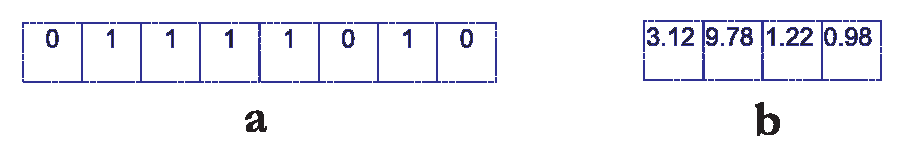
\includegraphics[scale=0.45]{Cap2/1-16.eps}
	  \caption{Ejemplo de un cromosoma binario (a) y otro real (b).}
      \label{fig:cromosoma}
      \end{figure}
  
  Llamamos \textit{gene} a una subcadena del cromosoma que codifica, com\'unmente, a un solo par\'ametro de dise\~no. Estos genes toman 
  ciertos valores, llamados \textit{alelos}, de alg\'un alfabeto gen\'etico. De esta manera, si usamos una representacion binaria, 
  los alelos 
  pueden tomar el valor de $0$ o de $1$. Un \textit{locus} define la posici\'on de un gene dentro del cromosoma (figura \ref{fig:gene}).

  \begin{figure}[H]
	\centering
	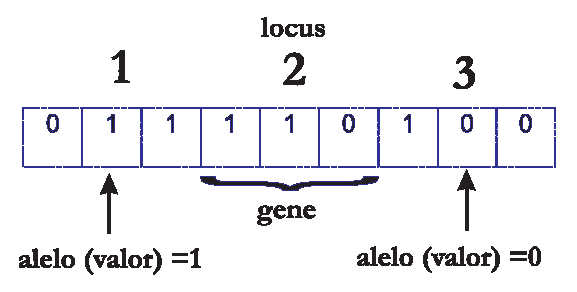
\includegraphics[scale=0.70]{Cap2/1-17.eps}
	  \caption{Cromosoma binario constituido por tres genes.}
      \label{fig:gene}
      \end{figure}
  
  Se denomina \textit{genotipo} a la codificaci\'on (por ejemplo, binaria, entera o real) de los par\'ametros de decisi\'on. Mientras 
  que \textit{fenotipo} es la decodificaci\'on del genotipo, con el fin de obtener los valores de los par\'ametros usados como entrada 
  en la funci\'on objetivo del problema que se trata (figura \ref{fig:genotipo}).

  \begin{figure}[H]
	\centering
	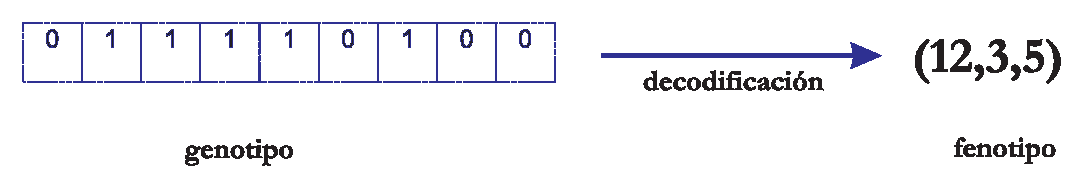
\includegraphics[scale=0.70]{Cap2/1-18.eps}
	  \caption{Decodificaci\'on del genotipo al fenotipo.}
      \label{fig:genotipo}
      \end{figure}
  
  Un \textit{individuo} es una soluci\'on potencial al problema que se trata. Cada individuo contiene un cromosoma. A un conjunto de individuos 
  se le nombra \textit{poblaci\'on}. La \textit{aptitud} de un individuo es la evaluaci\'on de la funci\'on de aptitud e indica qu\'e
  tan bueno es el individuo (es decir, la soluci\'on al problema) con respecto a los dem\'as.

  \subsection{Operadores evolutivos}
  
  Existe una amplia variedad de operadores que se han empleado en los algoritmos evolutivos. Algunos de ellos est\'an 
  dise\~nados especialmente para una clase particular de problemas. A continuaci\'on se describen los m\'as usados com\'unmente:
  
  \begin{itemize}
   \item \textbf{Selecci\'on}: la selecci\'on determina la probabilidad de elegir un individuo para que produzca descendencia por medio 
   de la recombinaci\'on y la mutaci\'on. El esquema de selecci\'on es una de las partes cruciales de un algoritmo evolutivo, puesto 
   que sesga la b\'usqueda de manera que eventualmente se llegue a la soluci\'on \'optima (o su proximidad).
   \item \textbf{Recombinaci\'on}: el operador de recombinaci\'on (cruza) tiene la finalidad de heredar la informaci\'on (genes) 
   de dos o m\'as padres a la descendencia. En la computaci\'on evolutiva la cruza entre cromosomas se simula intercambiando segmentos 
   de cadenas lineales de longitud fija. Lo usual es que las t\'ecnicas de cruza se apliquen sobre representaciones binarias; sin embargo, 
   con las modificaciones adecuadas, se pueden generalizar a alfabetos de cardinalidad mayor.
   \item \textbf{Mutaci\'on}: la mutaci\'on consiste en peque\~nas modificaciones al cromosoma de un individuo. En los 
   algoritmos gen\'eticos la mutaci\'on es considerada un operador secundario.
  \end{itemize}
  
  \subsection{Principales paradigmas}
  
  Actualmente existen, principalmente, tres paradigmas inspirados en los principios del \textit{neodarwinismo}: los \textit{algoritmos}
  \textit{gen\'eticos}, la \textit{programaci\'on} \textit{evolutiva} y las \textit{estrategias} \textit{evolutivas}. De manera gen\'erica, 
  a los algoritmos de la computaci\'on evolutiva se les llama \textit{algoritmos evolutivos}. Estas tres t\'ecnicas tienen en com\'un la 
  reproducci\'on, la variaci\'on aleatoria, la competencia y la selecci\'on de individuos contendientes dentro de una poblaci\'on. 
  
\begin{itemize}
 \item \textbf{Estrategias Evolutivas}: este modelo enfatiza los nexos conductuales entre padres e hijos, en lugar del nexo gen\'etico. 
 \'Estas fueron concebidas para construir sistemas capaces de resolver problemas de optimizaci\'on complejos en los que las variables
 son n\'umeros reales. Por ello, la representaci\'on natural fue un vector de genes con valores reales, el cual era manipulado, principalmente, 
 por operadores de mutaci\'on que perturbaban dichos valores reales \cite{Back97}.
 
 La primera versi\'on de una estrategia evolutiva, nombrada $(1+1)$-EE, crea un solo hijo a partir de un solo padre, y ambos compet\'ian
 para sobrevivir; el peor individuo era eliminado, mientras que el mejor se manten\'ia para la siguiente generaci\'on. En la $(1+1)$-EE, 
 a partir de un padre $x^{t}=(x_1, \ldots, x_n )$, el hijo se genera mediante la expresi\'on:

 \[x^{t+1}_i=x^{t} + N_i(0, \sigma^{t}_i)\]
 
donde $t$ se refiere a la generaci\'on actual, $i = 1, \ldots, n$ es la $i$-\'esima componente de los vectores $x$, $N$, $\sigma$ y
$\sigma^{t}_i$ es un n\'umero aleatorio gaussiano con media cero y desviaci\'on est\'andar $\sigma_i$ . Los n\'umeros aleatorios 
son generados de manera independiente.
 
 \item \textbf{Programaci\'on Evolutiva}: propuesta por Lawrence Fogel consideraba que el comportamiento inteligente requiere de dos 
 habilidades: la primera, a trav\'es de un organismo para poder hacer predicciones correctas dentro de su ambiente; y la segunda, 
 es la capacidad de traducir estas predicciones en una respuesta adecuada para una 
 meta dada. Los aut\'omatas de estados finitos fueron la representaci\'on ideal para modelar este comportamiento \cite{Fogel64}. 
 
 \item \textbf{Algoritmos Gen\'eticos}. Propuestos por \cite{Holland75}. Hay tres caracter\'isticas principales que los distinguen 
 de los dem\'as algoritmos evolutivos: la representaci\'on de los individuos (cadena binaria); el m\'etodo de selecci\'on (selecci\'on 
 proporcional); y el uso de la cruza como el operador principal para modificar al individuo. En este caso, la mutaci\'on es un operador 
  secundario.

\end{itemize}

\section{Optimizaci\'on multi-objetivo}
  
      Se define el problema de optimizaci\'on multi-objetivo como: ``La tarea de encontrar un vector de variables 
      de decisi\'on que satisfaga restricciones y optimice un vector de funciones objetivo. Esas funciones, generalmente est\'an
      en conflicto unas con otras y, describen matem\'aticamente un criterio de desempe\~no. Por lo tanto, el t\'ermino 
      optimizar significa encontrar un vector soluci\'on con valores aceptables para todas las funciones objetivo'' \cite{EASMC85}. 
      Los problemas multi-objetivo son aquellos en los que se deben optimizar $k \geq 2$ funciones objetivo simult\'aneamente. 
      El proceso de optimizaci\'on puede significar la maximizaci\'on de las $k$ funciones, la minimizaci\'on de las $k$ 
      funciones o una combinaci\'on de maximizaci\'on y minimizaci\'on de estas funciones.

      \begin{definicion}[Problema de Optimizaci\'on]
	  Un problema de optimizaci\'on multi-objetivo se define como la tarea de minimizar (o maximizar) 
	  
	  \[F\left(\vec{x}\right)=\left(f_1\left(\vec{x}\right), \ldots,f_k\left(\vec{x}\right) \right),\]
	  
	  {\setlength{\parindent}{0pt}
	  
	  donde $k\geq 2$ es el n\'umero de funciones a optimizar, sujetas a $g_i\left(\vec{x}\right) \leq 0 $ (restricciones de 
	  desigualdad) y $h_j\left(\vec{x}\right) = 0 $ (restricciones de igualdad) con $i = \left\{1, \ldots, m \right\}$, $j = \left\{1, \ldots, n \right\}$ 
	  y $\vec{x} \in \Psi $, donde $\vec{x}$ es un vector $n$-dimensional de variables de decisi\'on ($\vec{x} = \left(x_1 , \ldots, x_n \right) \in \Psi$). 
	  Las restricciones $g_i\left(\vec{x}\right) \leq 0$ y $h_j\left(\vec{x}\right) = 0$ deben ser satisfechas 
	  al mismo tiempo que se minimiza (o maximiza) $F\left(\vec{x}\right)$ y $\Psi $ contiene todos los posibles 
	  $\vec{x}$ que pueden ser usados para satisfacer la evaluaci\'on de $F\left(\vec{x}\right)$.
	  }
      \end{definicion}

      El vector de variables de decisi\'on puede ser continuo o discreto mientras que las $k$ funciones pueden ser 
      lineales o no, as\'i como continuas o discretas. La funci\'on de evaluaci\'on $F:\Psi \rightarrow \Omega$ es una transformaci\'on 
      del vector de variables de decisi\'on $\vec{x} = \left(x_1 , \ldots, x_n \right)$ en un vector de respuesta 
      $\vec{y} = \left(y_1 , \ldots, y_k \right)$. La figura ~\ref{fig:multiobj} muestra un problema de dos objetivos con dos variables.
      
      \begin{figure}
	\centering
	\includegraphics[scale=0.6]{Cap2/1-1.eps}
	  \caption{Un problema de dos objetivos con dos variables}
      \label{fig:multiobj}
      \end{figure}
            
      Cuando el problema es multi-objetivo existe un conflicto que ocasiona que la mejora en alg\'un objetivo provoque 
      el deterioro de otros. Por lo tanto, un problema de optimizaci\'on multi-objetivo consiste en encontrar el mejor 
      compromiso (balance) entre todos los objetivos. Las soluciones que representan los mejores compromisos entre los 
      objetivos se denominan \'optimos de Pareto.  
      
      \begin{definicion}[Optimalidad de Pareto]
	  Una soluci\'on $\vec{x}^*\in \Psi$ es un \'optimo de Pareto con respecto a $\Psi$ si y s\'olo si no existe 
	  $\vec{x}\in \Psi$, para la cual $\vec{v} = F\left(\vec{x}\right)=\left(f_1\left(\vec{x}\right), \ldots,f_k\left(\vec{x}\right) \right)$ 
	  domina a $\vec{u}^*=F\left(\vec{x}^*\right)=\left(f_1\left(\vec{x}^*\right), \ldots,f_k\left(\vec{x}^*\right) \right)$.
      \end{definicion}
      
      \begin{definicion}[Dominancia de Pareto]
	  Un vector $\vec{u} = \left(u_1, \ldots, u_k \right)$ se dice que domina a $\vec{v} = \left(v_1, \ldots, v_k \right)$,
	  denotado por $\vec{u} \preceq \vec{v}$, si y s\'olo si $\vec{u}$ es parcialmente menor que $\vec{v}$, es decir, 
	  $\forall i \in \left\{1, \ldots, k \right\}: u_i \leq v_i \wedge \exists i \in \left\{1, \ldots, k\right\}: u_i < v_i$.
      \end{definicion}
    
      La figura \ref{fig:paretodominance} muestra gr\'aficamente la dominancia de Pareto para un problema de optimizaci\'on
      con dos objetivos en el cual $A \preceq C$ tal que $A$ es mejor en ambas funciones, $A \preceq E$ tal que $A$ es igual con respecto 
      a $f_2$ pero es mejor con respecto a $f_1$, $B \preceq E$ tal que $B$  es igual con respecto a $f_1$ pero mejor con respecto a 
      $f_2$, $B\preceq D$ tal que B es mejor en ambas funciones, y $A$ y $B$ son incomparables ($A$ y $B$ son \'optimos de Pareto).
       
       \begin{figure}
	\centering
	\includegraphics[scale=0.6]{Cap2/1-4.eps}
	  \caption{Dominancia de Pareto}
      \label{fig:paretodominance}
      \end{figure}
       
      \begin{definicion}[Conjunto de \'optimos de Pareto]
	Para un problema multi-objetivo determinado $F\left(\vec{x}\right)$, el conjunto de \'optimos de Pareto, denotado por $P^*$ 
	o $P_{real}$, est\'a definido como:	
	\[
	P^*= \left\{ \vec{x} \in \Psi |\hspace{0.3cm} \nexists \vec{y}\in \Psi \hspace{0.7cm} F\left(\vec{y}\right)\preceq F\left(\vec{x}\right) \right\}\]
      \end{definicion}
      
      Los elementos del conjunto de \'optimos de Pareto tienen vectores objetivo que no pueden ser mejorados sin empeorar al menos otro
      objetivo. Los vectores objetivo de las soluciones \'optimas de Pareto se denominan vectores (o soluciones) \textit{no dominados}.
      Los vectores de las funciones objetivo correspondientes al conjunto de \'optimos de Pareto conforman el denominado frente de Pareto 
      ($\mathcal{F}^*$).
      
      \begin{definicion}[Frente de Pareto]
      Para un problema multi-objetivo determinado $F\left(\vec{x} \right)$, siendo su conjunto de \'optimos de Pareto ($P^*$) , el Frente 
      de Pareto $\mathcal{F}^*$ o $\mathcal{F}_{real}$, est\'a definido como (ver figura \ref{fig:pareto}):
      
	  \[\mathcal{F}^*=\left\{ \vec{u} = F\left(\vec{x}\right) | \hspace{0.3cm} \vec{x}\in P^*\right\}\]
      \end{definicion}
      
      \begin{figure}
	\centering
	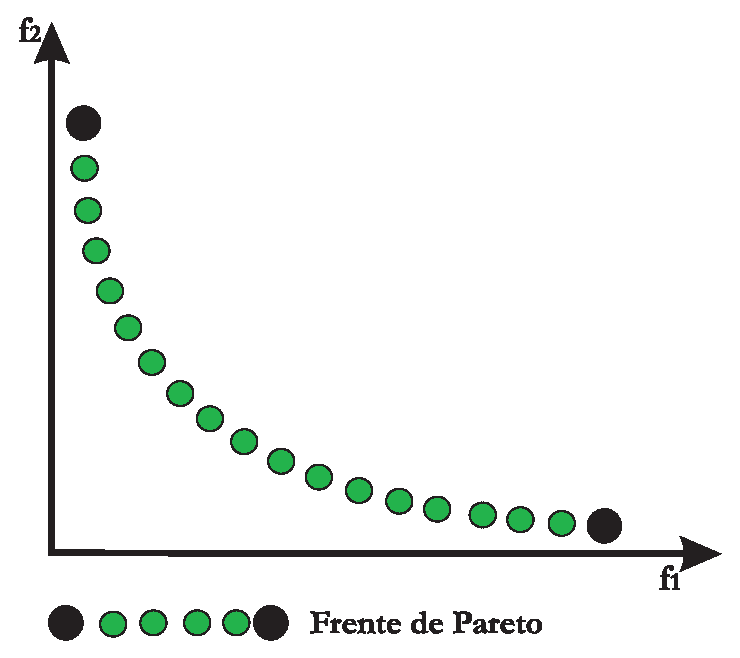
\includegraphics[scale=0.65]{Cap2/1-2.eps}
	  \caption{Frente de Pareto}
      \label{fig:pareto}
      \end{figure}
      
      \begin{definicion}[Vector Ideal y vector de Nadir]
      Para un problema multi-objetivo determinado $F\left(\vec{x}\right)$, siendo su conjunto de \'optimos de Pareto, $P^*$, 
      el vector ideal se define como (ver figura \ref{fig:ideanadir}):
      
      \[  f_{ideal}= \left(^{\min}_{\vec{x}\in P^*}f_1\left(\vec{x}\right), \ldots, ^{\min}_{\vec{x}\in P^*}f_k\left(\vec{x}\right) \right)\]
      
      Si el vector ideal de un problema es alcanzabe, entonces los objetivos del problema no est\'an en conflicto 
      y la soluci\'on del problema es \'unica. Por lo tanto, cada objetivo del problema puede ser optimizado por separado,
      sin requerirse el uso de un algoritmo evolutivo multi-objetivo.
      De manera similar, el vector de Nadir se define como (ver figura \ref{fig:ideanadir}):
      
      \[  f_{nadir}= \left(^{\max}_{\vec{x}\in P^*}f_1\left(\vec{x}\right), \ldots, ^{\max}_{\vec{x}\in P^*}f_k\left(\vec{x}\right) \right)\]
      
      Este vector contiene, entonces, los peores valores de las funciones objetivo y suele usarse (junto al vector ideal)
      para acotar el frente de Pareto.      
      
      \end{definicion}
      
      \begin{figure}
	\centering
	\includegraphics[scale=0.65]{Cap2/1-3.eps}
	  \caption{Vector Ideal y vector de Nadir}
      \label{fig:ideanadir}
      \end{figure}
      
      \subsection{M\'etricas para evaluar la eficacia}
      \label{sec:metric}
      Al trabajar en optimizaci\'on multi-objetivo, se tienen que tomar en cuenta dos nociones importantes: la convergencia y la 
      dispersi\'on. Para medir la convergencia, se debe de estimar qu\'e tan lejos est\'an las soluciones que generamos del
      verdadero frente de Pareto y para medir la dispersi\'on, se debe estimar qu\'e tan uniformemente est\'an distribuidos 
      las soluciones a lo largo del frente de Pareto. Para medir la convergencia se pueden usar medidas como las siguientes:
      
      \begin{definicion} [Distancia Generacional Invertida (IGD)]
      Determina cu\'an lejos, en promedio, se encuentra el verdadero frente de Pareto, del frente obtenido por el algoritmo.
      Esta m\'etrica evita algunos problemas que posee la denominada Distancia Generacional, en particular, en los casos en 
      los que el frente obtenido posee pocos puntos, pero agrupados en una sola regi\'on \cite{Veldhuizen98}. 
      Su definici\'on es la siguiente:

      \[
	IGD = \frac{1}{N} \cdot \sqrt{\sum^{N}_{i=1}{d^2_i}},
      \]
      {\setlength{\parindent}{0pt}
      donde $N$ es la cantidad de puntos del verdadero frente de Pareto, $d_i$ la distancia euclidiana (medida en el espacio 
      de las funciones objetivo) entre cada punto del verdadero frente, al punto m\'as cercano del frente obtenido. Un valor 
      $IGD = 0$ indica que el frente obtenido es el verdadero frente de Pareto, cualquier otro valor indica que el frente obtenido 
      se desv\'ia del verdadero frente de Pareto.
      }
      \end{definicion}
  
      \begin{definicion}[Cobertura de Conjuntos ($\mathcal{C}$)]
	  Determina la cobertura relativa de un conjunto, con respecto a otro. Fue propuesta por \cite{Zitzler2000} para 
	  valorar cuantitativamente cu\'anto un conjunto cubre o domina a otro. Si $A$ y $B$ son dos conjuntos no dominados,
	  la m\'etrica de cobertura de $\mathcal{C}(A,B)$ calcula la fracci\'on de vectores en $B$ que son dominados 
	  d\'ebilmente por los vectores de $A$. Se define como:

	  \[
	      \mathcal{C}\left(A, B \right) = \frac{|\vec{b} \in B; \exists \vec{a} \in A: \vec{a}\preceq \vec{b}|}{|B|}
	  \]
	  
	  Si todos los vectores en $B$ son dominados o son iguales a los vectores en $A$, entonces $\mathcal{C}$ es igual a uno. 
	  Si ninguno de los vectores en $B$ es dominado o igual a alg\'un vector de $A$, entonces $\mathcal{C}$ es igual a cero. 
	  Lo ideal es que $\mathcal{C} \left(A, B\right)$  y $\mathcal{C} \left(B, A \right)$ se consideren de manera separada, 
	  ya que $\mathcal{C}\left(A, B\right)$ no es equivalente a $1- \mathcal{C}\left(B, A\right)$
      \end{definicion}
      
      \begin{definicion}[Dispersi\'on o Espaciamiento (Spread) (S)]
	 Determina la dispersi\'on de los puntos sobre el frente. Fue utilizada por \cite{deb02} para conocer 
	 c\'omo est\'an distribuidas las soluciones a lo largo del frente de Pareto. Se define como:
	 
	 \[S= \frac{d_f + d_l + \sum^{N-1}_{i=1}{|d_i-d^{'}|}}{d_f + d_l + \left(N -1\right)\cdot d^{'}}\]
  
      donde $N$ es la cantidad de puntos del frente, $d_i$ es la distancia euclidiana entre soluciones consecutivas, 
      $d^{'}$ es el valor medio de todas las distancias y, $d_f$ y $d_l$ son las distancias euclidianas a los extremos 
      del frente de Pareto. Un valor $S = 0$ indica la distribuci\'on ideal (dispersi\'on perfecta).
      \end{definicion}   
      
      La dispersi\'on indica qu\'e tan bien est\'an distribuidas las soluciones en el verdadero frente de Pareto (o su aproximaci\'on).
      Este indicador es importante, ya que ofrece m\'as opciones para la toma de decisiones al momento de elegir una o m\'as soluciones 
      no dominadas.
  
  \subsection{Algoritmos evolutivos multi-objetivo}

  Hoy en d\'ia existen diversas t\'ecnicas de programaci\'on matem\'atica para resolver problemas de optimizaci\'on multi-objetivo 
  \cite{Miettinen98, EASMC85}. Sin embargo, la complejidad de muchos problemas de optimizaci\'on multi-objetivo del mundo real vuelven 
  a estas t\'ecnicas inadecuadas o incluso inaplicables para resolverlos. La complejidad de estos problemas se debe, por ejemplo a: 
  la multimodalidad, la alta dimensionalidad del espacio de b\'usqueda, a la discontinuidad de las funciones objetivo, a desconexiones 
  tanto en el espacio de la variables de decisi\'on como en el de las funciones objetivo, entre otras causas.

  Rosenberg plante\'o utilizar un m\'etodo gen\'etico de b\'usqueda para resolver problemas de optimizaci\'on
  multi-objetivo por primera vez, pero no lleg\'o a desarrollar un algoritmo, dado que transform\'o el problema 
  bi-objetivo de su inter\'es en uno mono-objetivo \cite{Rosenberg67}. La primera implementaci\'on de lo que 
  actualmente se conoce como un algoritmo evolutivo multi-objetivo fue propueta por \cite{Schaffer84}. 

  Los algoritmos evolutivos resultan particularmente adecuados para resolver problemas de optimizaci\'on multi-objetivo gracias a que
  trabajan simult\'aneamente con un conjunto de soluciones potenciales (es decir, la poblaci\'on). Esta caracter\'istica les permite 
  encontrar varias soluciones del conjunto de \'optimos de Pareto en una sola ejecuci\'on. Tambi\'en, son menos sensibles a la forma o 
  continuidad del frente de Pareto. Adicionalmente, son f\'aciles de usar y no requieren informaci\'on espec\'ifica del problema a resolverse.

  Los algoritmos evolutivos y los algoritmos evolutivos multi-objetivo son estructuralmente similares. La diferencia principal es que 
  los segundos utilizan un esquema de selecci\'on que debe considerar $k$ ($k \geq 2$) funciones objetivo, adem\'as de contar
  con un estimador densidad en el espacio de las funciones objetivo que sesga el mecasnimo de selecci\'on de manera 
  que se mantenga diversidad en la poblaci\'on. 
  Sin embargo, el operador de selecci\'on espera un solo valor de aptitud. La forma m\'as sencilla de mantener 
  la estructura de un algotirmo evolutivo simple al abordar problemas multi-objetivo (si bien, no es la m\'as adecuada) consiste en 
  transformar el vector de aptitudes en un valor escalar. En el algoritmo \ref{alg:AEb} se describe una estructura b\'asica de un 
  algoritmo evolutivo multi-objetivo, de este tipo. N\'otese que este algoritmo no incluye un estimador de densidad.
  
  \begin{algorithm}
      \begin{algorithmic}[1]			
	\STATE $t \leftarrow 0$.
	\STATE Generar aleatoriamente la poblaci\'on inicial $P^t$.
	\WHILE{$t < max_{Gen}$}
	\STATE Para cada individuo $\vec{x} \in P^t$ calcular el valor escalar de aptitud $F(\vec{x})$.
	\STATE Seleccionar de $P^t$ un grupo de padres $P'^t$ bas\'andose en la aptitud.
	\STATE Recombinar los individuos de $P'^t$ para obtener $P''^t.$
	\STATE Mutar los individuos de $P''(t)$ para obtener $P'''^t$.
	\STATE $P^{t+1 } \leftarrow P'''^t$.
	\STATE $t\leftarrow t +1$.
	\ENDWHILE 
  \end{algorithmic}
  \caption{Estructura b\'asica de un algoritmo evolutivo multi-objetivo agregativo}
  \label{alg:AEb}
  \end{algorithm}

  En general, existen diferentes esquemas para manejar varias funciones objetivo en la selecci\'on: los basados en agregaci\'on, los basados 
  en poblaciones, y los basados en el concepto de dominancia de Pareto \cite{Zitzler99}. Otro componente fundamental de los algoritmos
  evolutivos multi-objetivo modernos es el elitismo.

  Actualmente hay dos formas principales de llevar a cabo la implementaci\'on del elitismo en un algoritmo evolutivo multi-objetivo. La primera,
  es combinar la poblaci\'on anterior y la descendencia o la poblaci\'on nueva, y posteriormente aplicar una selecci\'on determinista 
  en lugar de reemplazar la vieja poblaci\'on por la descendencia \cite{deb02}. La segunda, es mantener una poblaci\'on secundaria 
  llamada archivo hist\'orico (poblaci\'on secundaria, poblaci\'on elitista o archivo externo) en el cual se retienen las soluciones no 
  dominadas encontradas en el transcurso del proceso de b\'usqueda \cite{Zitzler99}(ver figura \ref{fig:elitismo}). En muchos problemas 
  de optimizaci\'on multi-objetivo, el conjunto de \'optimos de Pareto es muy grande. Por ello, se debe aplicar una estrategia para decidir 
  la entrada de la nuevas soluciones al archivo y evitar que el archivo crezca indefinidamente.
  
    \begin{figure}[H]
	\centering
	\includegraphics[scale=0.60]{Cap2/1-19.eps}
	  \caption{Dos esquemas para llevar a cabo el elitismo.}
      \label{fig:elitismo}
      \end{figure}
  
  \subsection{Clasificaci\'on}
  
  Existen diferentes maneras de clasificar a los algoritmos evolutivos multi-objetivo. Quiz\'as la taxonom\'ia m\'as simple, 
  es la basada en el tipo de mecanismo de selecci\'on que usan \cite{EASMC}:
  
  \begin{itemize}
   \item \textbf{Enfoques basados en agregaci\'on}. Esta t\'ecnica simplemente combina todos los objetivos 
   en un valor escalar, es decir, transforman 
   un problema de optimizaci\'on multi-objetivo en un problema de optimizaci\'on mono-objetivo. Para ello se usa la siguiente 
   expresi\'on: 
   
	\[ \min {\sum^{k}_{i=1}{w_i\cdot f_i\left(\vec{x}\right)}}\]
   
   donde $w_i > 0$ son los coeficientes de ponderaci\'on que representan la importacia de cada cada objetivo $k$ del
   problema. Usualmente se presupone que:
   
   \[\sum^{k}_{i=1}{w_i}=1\]
   
   Las funciones agregativas lineales tienen diversos inconvenientes, entre los que destaca el hecho de no 
   poder generar partes no convexas del frente de Pareto. Las funciones agregativas no lineales no tienen esta limitante,
   pero no son muy comunes en la literatura especializada. Pese a sus limitantes, las funciones agregativas han sido utilizadas
   con \'exito en problemas combinatorios multi-objetivo.
   
   \item \textbf{Enfoques basados en poblaci\'on}. En este tipo de enfoque, la poblaci\'on se utiliza para la diversificaci\'on de la b\'usqueda, 
   pero el concepto de dominancia de Pareto no se incorporan directamente en el proceso de selecci\'on. Un ejemplo cl\'asico es el 
   algoritmo \textbf{VEGA} (\textit{Vector Evaluated Genetic Algorithm}) \cite{Schaffer84}. VEGA consiste en un algoritmo gen\'etico 
   con un mecanismo de selecci\'on modificado. En cada generaci\'on, se crea un n\'umero de sub-poblaciones de acuerdo con una 
   selecci\'on proporcional a cada objetivo por cada funci\'on a la vez. Estas sub-poblaciones son luego mezcladas entre s\'i para 
   obtener una nueva poblaci\'on, en la que el algoritmo gen\'etico aplica los operadores de cruza y mutaci\'on. VEGA tiene varios 
   problemas, del cual se puede destacar el que su esquema de selecci\'on se opone al concepto de dominancia de Pareto.
   
   \item \textbf{Enfoques basados en optimilidad de Pareto}. En este tipo de enfoque, se consideran los algoritmos evolutivos multi-objetivo que 
   incorporan el concepto de Pareto en su mecanismo de selecci\'on. Los siguentes algoritmos evolutivos son un conjunto representativo 
   que utilizan este enfoque en los \'ultimos a\~nos:
   
   \begin{itemize}
    \item \textbf{PAES (\textit{The Pareto Archived Evolution Strategy})}: este m\'etodo consiste en una estrategia evolutiva (1+1),
    en combinaci\'on con un archivo hist\'orico que almacena algunas de las soluciones no dominadas encontradas previamente. Este
    archivo es usado como un conjunto de referencia contra el cual se compara cada individuo mutado. PAES tambi\'en utiliza un nuevo 
    enfoque de mantener diversidad, que consiste de un procedimiento de agrupamiento que divide el espacio de las funciones objetivo 
    de una manera recursiva. Cada soluci\'on se situa en una rejilla de localizaci\'on, con base en los valores de las funciones
    objetivo. Se mantiene un mapa en dicha rejilla y un conteo del n\'umero de soluciones que residen en cada ret\'icula de la misma.
    Dado que el procedimiento es adaptivo, no se requieren par\'ametros extras en el algoritmo \cite{paes99}.
    
    \item \textbf{NSGA (\textit{The Nondominated Sorting Genetic Algorithm})}: este m\'etodo clasifica a los 
    individuos de la poblaci\'on en varias capas. Antes de hacer la selecci\'on, la poblaci\'on se clasifica conforme a 
    su no dominancia: todos los individuos no dominados se clasifican en una categor\'ia con un valor ficticio de 
    aptitud el cual es proporcional al tama\~no de la poblaci\'on, para ofrecer el potencial reproductivo de estos 
    individuos \cite{Srinivas94}. NSGA es un algoritmo no elitista. La siguiente versi\'on de este algoritmo, es el \textbf{NSGA-II}, 
    que utiliza el elitismo y un operador de comparaci\'on que clasifica a la poblaci\'on conforme a la dominancia de Pareto y 
    la densidad de la regi\'on. Por lo que, este algoritmo es m\'as eficiente y efectivo que su predecesor.
    
    \item \textbf{SPEA (\textit{The Strength Pareto Evolutionary Algorithm})}: este m\'etodo introduce elitismo al almacenar a los
    individuos no dominados en un archivo. Para cada individuo de este conjunto externo se calcula un valor llamado fortaleza 
    (\textit{strength}). Este valor es proporcional al n\'umero de soluciones que domina un cierto individuo del conjunto externo.
    La aptitud de los miembros de la poblaci\'on actual se calcula de acuerdo a la fortaleza de los individuos de la poblaci\'on
    externa que lo dominan. En este esquema el objetivo es minimizar la aptitud, es decir, los valores peque\~nos de aptitud corresponden 
    a altas probabilidades 	de reproducci\'on. El esquema para asignar la aptitud pretende conseguir que la b\'usqueda 
    se dirija hacia el frente de Pareto y a la vez preservar la diversidad de las soluciones no dominadas. Para proveer 
    diversidad a la poblaci\'on, se utiliza una t\'ecnica de c\'umulos (\textit{clustering}), llamada m\'etodo de enlace 
    promedio \cite{Zitzler99}. 
    
    La siguiente versi\'on de este algoritmo, es el \textbf{SPEA2}, el cual tiene las siguientes diferencias \cite{zlt2002a}:
   
    \begin{itemize}
     \item Incorpora una estrategia de asignaci\'on de aptitud de grano-fino, que por cada individuo toma en cuenta
     el n\'umero de individuos a los que domina y el n\'umero de individuos por los cuales es dominado.
     \item Utiliza una t\'ecnica de estimaci\'on del vecino m\'as cercano que gu\'ia  la b\'usqueda de una manera
     m\'as efectiva.
     \item Presenta un m\'etodo mejorado de truncamiento del archivo, que garantiza  la preservaci\'on de las 
     soluciones de los extremos del frente de Pareto.
     \item Utiliza un algotitmo de \textit{clustering} de menor complejidad.
    \end{itemize}    
   \end{itemize}
\end{itemize}

  Como se mostr\'o anteriormente en la literatura existen muchas formas de poder resolver problemas multi-objetivo utilizando 
  diversos enfoques. En este trabajo de investigaci\'on se plantea comparar el desempe\~no del algoritmo propuesto con respecto a 
  las soluciones obtenidas con los siguientes algoritmos reprensetativos de la literatura especializa:
  
  \begin{itemize}
   \item El primero, es el que presentan \cite{Raquel2005} en el cual se 
  plantea el uso de un algoritmo de c\'umulos de part\'iculas para problemas multi-objetivo (\textit{An effective use of Crowding Distance 
  in Multiobjetive Particle Swarm Optimization}, \textbf{MOPSOcd}) mediante la incorporaci\'on del mecanismo del c\'alculo de la distancia 
  de \textit{Crowding} espec\'ificamente para seleccionar al mejor l\'ider global y en el m\'etodo para mantener las soluciones no dominadas 
  en el archivo externo. El algoritmo \ref{alg:MOPSOcd} muestra la estructura b\'asica del MOPSOcd.
  
  Las caracter\'isticas que enmarcan al algoritmo MOPSOcd son:
  
  \begin{itemize}
   \item Hace uso de un operador de mutaci\'on junto a la distacia de \textit{Crowding} para mantener la 
  diversidad de soluciones no dominadas en un archivo externo.  
  \item La selecci\'on del mejor l\'ider global se hace de entre aquellas soluciones 
  no dominadas con los valores m\'as altos de la distancia de \textit{crowding} (por ejemplo, 10\% de  la parte superior 
  del archivo ordenado de manera desdente). 
  \item La selecci\'on de diferentes gu\'ias para cada part\'icula en una parte determinada del archivo 
  de soluciones no dominadas ordenadas en funci\'on de las distancia de \textit{crowding} 
  (por ejemplo, 10\% de  la parte inferior del archivo)
  permite que las part\'iculas de la poblaci\'on primaria avancen hac\'ia las soluciones no dominadas del archivo externo con el menor 
  agrupamiento en el espacio de las funciones objetivo. 
  \item Los resultados muestran que este algoritmo es competitivo en lo que a 
  convergencia hacia el frente de Pareto se refiere, generando tambi\'en un conjunto bien distribuido de soluciones no dominadas. 
  \item Adapta un mecanismo de manejo de restricciones usado por el NSGA-II, debido a su simplicidad en la factibilidad y la comparaci\'on 
  de soluciones no dominadas.
  \end{itemize}  
 
\begin{algorithm}
      \begin{algorithmic}[1]			
	    \REQUIRE Problema de Optimizaci\'on $F$.
	\ENSURE Soluciones no dominadas en un archivo acotado $A$.	  	  
	  \STATE Inicializar la velocidad $\vec{v} \leftarrow 0$ del c\'umulo $S$.
	  \STATE Inicializar aleatoriamente las posiciones del c\'umulo $S$.
	  \STATE Evaluar las part\'iculas del c\'umulo $S$ de acuerdo a las funciones objetivo.
	  \STATE Seleccionar el $pBest$ inicial de las part\'iculas.
	  \STATE Seleccionar el $\vec{gBest}$ como el mejor encontrado en el c\'umulo $S$.
	  \STATE Inicializar el contador de generaciones con $t \leftarrow 0$.
	  \STATE Insertar las part\'iculas no dominadas de la poblaci\'on en el archivo $A$.	  
	\WHILE {$t < max_{Gen}$}
	  \STATE Calcular la distancia de \textit{crowding} de cada part\'icula no dominada en el archivo $A$
	  \STATE Ordenar las part\'iculas no dominadas en el archivo $A$ de manera descendiente de acuerdo a los valores 
	     de \textit{crowding}.	   
	  %\\ Calcular la nueva velocidad y posici\'on de cada part\'icula en la poblaci\'on.
	  \FOR {$i\leftarrow 1$ hasta $tam_S$}
	      \STATE Seleccionar aleatoriamente el $\vec{gBest}$ desde una porci\'on especificada (por ejemplo, $10\%$ de la parte superior) 
	      del archivo ordenado $A$.
	     \STATE Generar una nueva velocidad 
		\\  $\vec{v}^{t+1}_{i} \leftarrow \omega \cdot \vec{v}^t_{i} + \phi_1 \cdot rnd_1 \cdot \left(\vec{pBest}t^t_i - \vec{S}^t_{i} \right) 
					    + \phi_2 \cdot rnd_2 \cdot \left(\vec{gBest} - \vec{S}^t_{i} \right)$	
	      \STATE Calcular las nuevas posiciones 
		\\$\vec{S}^{t+1}_{i} \leftarrow \vec{S}^{t}_{i}+\vec{v}^{t+1}_{i}$
	      \STATE Reintegrar la part\'icula $i$ si no pertenece a la regi\'on de b\'usqueda y la velocidad de esta part\'icula se 
	      multiplica por $-1$.	      
	      \IF {$t < max_{Gen}\cdot pMut$}
		\STATE Aplicar el operador de mutaci\'on en la part\'icula $i$.
	      \ENDIF
	      \STATE Evaluar la part\'icula $i$ de acuerdo a las funciones objetivo.
	     \ENDFOR					  
	  \STATE Insertar todas las past\'iculas no dominadas de $S$ en $A$ si no son dominadas por alguna part\'icula ya almacenada.
	  Todas las part\'iculas en el archivo que sean dominadas por la nueva part\'icula son eliminadas. Si el archivo esta lleno,
	  las part\'iculas se reemplazan de acuerdo al siguiente criterio:
	    \begin{itemize}
	       \item Calcular la distancia de \textit{Crowding} de cada part\'icula no dominada del archivo $A$.
	       \item Ordenar las part\'iculas no dominadas en el archivo $A$ de manera descendiente de acuerdo a los valores 
	       \item Seleccionar aleatoriamente una part\'icula desde una porci\'on espeficada (por ejemplo, $10\%$ de la parte inferior) 
	       del archivo ordenado $A$, las cuales comprenden las part\'iculas m\'as agrupadas en el archivo y luego sustituirla por la 
	       nueva part\'icula.
	      \end{itemize}	  
	  \STATE Actualizar el $pBest$ de cada part\'icula en $S$. Si el actual $pBest$ domina la posici\'on en memoria, la posici\'on de la 
	  es actualizada utilizando $pBest \Leftarrow S$
	  \STATE $t \leftarrow t + 1$.
	\ENDWHILE
      \end{algorithmic}
  \caption{Estructura b\'asica del MOPSOcd}
  \label{alg:MOPSOcd}
  \end{algorithm}
 
 
  \item El segundo, es un algoritmo cuyo mecanismo de selecci\'on adopta el hipervolumen, llamado \textit{S metric selection 
  evolutionary multiobjective algorithm} (\textbf{SMS-EMOA}) propuesto 
  por \cite{Beume07}. Este algoritmo genera en cada iteraci\'on nuevas soluciones por medio de operadores de variaci\'on aleatoria. 
  Por tanto, las soluciones se descartan conforme a su contribuci\'on al hipervolumen. Los resultados muestran que el SMS-EMOA es muy 
  potente para problemas dif\'iciles. Su principal inconveniente es su alta complejidad computacional, que est\'a relacionada con el 
  c\'alculo de la contribuci\'on al hipervolumen que puede tomar mucho tiempo conforme se aumenta el n\'umero de objetivos.
   El algoritmo \ref{alg:SMS-EMOA} muestra la estructura b\'asica del SMS-EMOA.

   Los pilares principales que enmarcan al algoritmo SMS-EMOA son:
   
   \begin{itemize}
    \item El ordenamiento no dominado con base en los niveles o jerarqu\'ias de no dominancia ($rank$) usado por el NSGA-II.
    \item El hipervolumen se aplica como criterio de selecci\'on para descartar individuos.
   \end{itemize}
  
  \begin{algorithm}
      \begin{algorithmic}[1]			
	\REQUIRE Problema de Optimizaci\'on $F$.
	\ENSURE Una aproximaci\'on al frente de Pareto.
	\STATE $t \leftarrow 0$
	\STATE Inicializar la poblaci\'on aleatoriamente $P_t$
	\WHILE {criterio de paro}
	    \STATE Generar un nuevo individuo $x$ de acuerdo con un operador de variaci\'on aleatoria.
	    \STATE $Q_{t+1}\leftarrow P_t \cup \left\{x \right\}$.
	    \STATE Calcular el frente de Pareto de acuerdo con la asignaci\'on de valores de aptitud con base en los niveles o jerarqu\'ias 
	    de no dominancia ($rank$) de $Q_{t+1}$.
	    \STATE $W \leftarrow$ individuos con la peor clasificaci\'on del frente.
	    \STATE $r \leftarrow$ individuos (en $W$) que menos contribuyen al valor del hipervolumen cubierto por $W$.
	    \STATE $P_{t+1}\leftarrow Q_{t+1} \diagup r$, eliminar los peores inviduos detectados de la poblaci\'on.
	    \STATE $t \leftarrow t +1$.
	\ENDWHILE
      \end{algorithmic}
  \caption{Estructura b\'asica del SMS-EMOA}
  \label{alg:SMS-EMOA}
  \end{algorithm}
 
  \item Por \'ultimo, pero no menos importante, est\'a el \textbf{NSGA-II} el cual ha sido muy popular 
  en la literatura especialzada debido,  sobre todo, a su eficiencia y facilidad de uso. Este algoritmo tiene tambi\'en un bajo 
  costo computacional, bas\'andose en un operador de agrupamiento (\textit{Crowding}) y un esquema de selecci\'on que compara la 
  poblaci\'on de padres con la de hijos qued\'andose con los mejores individuos de entre todos ellos \cite{deb02}. 
  El algoritmo \ref{alg:NSGA-II} muestra la estructura b\'asica del NSGA-II.
  
  Las caracter\'isticas que enmarcan al algoritmo NSGA-II son:
  
  \begin{itemize}
   \item El ordenamiento no dominado mediante una t\'ecnica de comparaci\'on que utiliza una subpoblaci\'on auxilizar.
   \item El uso de una t\'ecnica de agrupaci\'on, que no requiere especificar par\'ametros adicionales para la preservaci\'on
   de la diversidad en la poblaci\'on.
   \item La asignaci\'on de valores de aptitud con base en los niveles o jerarqu\'ias de no dominancia ($rank$), aunque se considera 
   en el procedimiento de asignaci\'on de valores de distancia de \textit{crowding} utilizados para evaluar la diversidad de las 
   soluciones.
  \end{itemize}


  
  \begin{algorithm}
      \begin{algorithmic}[1]			
	\REQUIRE Problema de Optimizaci\'on $F$.
	\ENSURE Una aproximaci\'on al frente de Pareto.
	\STATE $t\leftarrow0$
	\STATE Inicializar la poblaci\'on $P_t$
	\WHILE {$t < max_{Gen}$}
	    \STATE Aplicar cruza y mutaci\'on a $P_t$, para generar $Q_t$
	    \STATE Evauar poblaci\'on $Q_t$ de acuerdo a las funciones objetivo
	    \STATE $R_t \leftarrow P_t \cup Q_t$
	    \STATE Asignar gerarquias con base en la dominacia de Pareto a $R_t$
	    \STATE Asignar distancia de agrupamiento a $R_t$
	    \STATE Seleccionar los $N$ individuos de $R_t$, de acuerdo al operador de comparaci\'on de agrupamiento
	    $\prec_n$ para obtener $P_{t+1}$.
	    \STATE $t  t +1$
	\ENDWHILE
      \end{algorithmic}
  \caption{Estructura b\'asica del NSGA-II}
  \label{alg:NSGA-II}
  \end{algorithm}

  
  \end{itemize}
  A continuaci\'on se describe m\'as a detalle el algoritmo basado en c\'umulos de part\'iculas.
      
\section{Algoritmo basado en c\'umulos de part\'iculas}

  El algoritmo de optimizaci\'on mediante c\'umulos de part\'iculas fue propuesto en 1995 us\'andose originalmente
  para el balance de pesos de una red neuronal. A continuaci\'on se describen las principales componentes de la heur\'istica, 
  los modelos mono-objetivo m\'as caracter\'isticos y, finalmente, como llevar \'esta misma a su versi\'on multi-objetivo.

  \subsection{Paradigma}
  
  Un algoritmo basado en c\'umulos de part\'iculas o \textit{Particle Swarm Optimization (PSO)} es una t\'ecnica inspirada en el 
  comportamiento social del vuelo de las aves o el movimiento de los bancos de peces que intentan encontrar comida. Se fundamenta 
  en los factores que influyen en la toma de decisiones de una part\'icula que forma parte de un c\'umulo de part\'iculas similares. 
  La decisi\'on de cada part\'icula se realiza conforme a una componente social y una componente individual, mediante las que se 
  determina el movimiento (direcci\'on) para alcanzar una nueva posici\'on en el espacio de soluciones. La met\'afora se puede resumir 
  de la siguiente forma: ``los individuos que conviven en una sociedad tienen una opini\'on que es parte de un conjunto de creencias 
  (el espacio de b\'usqueda) compartido por todos los posibles individuos'' \cite{JKennedySI}. 
  
  Siguiendo ciertas reglas de interacci\'on, las part\'iculas en la poblaci\'on adaptan sus esquemas de creencias al de las part\'iculas 
  con m\'as \'exito de su entorno. Con el tiempo, surge una cultura de creencias estrechas entre los individuos. Cada soluci\'on 
  (part\'icula) es un ave en el espacio de b\'usqueda que est\'a 
  siempre en continuo movimiento y que nunca muere. El c\'umulo de part\'iculas (\textit{Swarm}) es un sistema multiagente; es decir, 
  las part\'iculas son agentes simples que se mueven por el espacio de b\'usqueda y que guardan (y posiblemente comunican) la mejor soluci\'on 
  que han encontrado hasta el momento. Cada part\'icula tiene una posici\'on y un vector velocidad que dirige su movimiento. El movimiento 
  de las part\'iculas por el espacio est\'a guiado por las part\'iculas \'optimas en el momento actual.
  
  Esta heur\'istica posee las siguientes caracter\'itisticas \cite{JKRBParticle}: En primer lugar, asume un intercambio de informaci\'on 
  (interacciones sociales) entre las part\'iculas de b\'usqueda. Es decir, las part\'iculas modifican su direcci\'on en funci\'on 
  de las direcciones de las part\'iculas de su vecindario. Adem\'as, almacena informaci\'on hist\'orica de la experiencia propia 
  de cada part\'icula (influencia individual). Cada part\'icula decide su nueva direcci\'on en funci\'on de la mejor posici\'on 
  por la que pas\'o anteriormente. Suele tener una convergencia r\'apida a buenas soluciones.
  
  Tambi\'en comparte otras caracter\'isticas con los algoritmos evolutivos, tales como:
  
  \begin{itemize}
   \item La poblaci\'on es inicializada aleatoriamente y evoluciona iterativamente buscando la mejor soluci\'on posible.
   \item Realiza una b\'usqueda ciega, es decir, no dispone de ning\'un conocimiento espec\'ifico del problema, de manera 
   que la b\'usqueda se basa exclusivamente en los valores de la funci\'on objetivo.
   \item Trabaja con informaci\'on codificada (binaria, entera o real), no directamente sobre el dominio del problema, sino sobre 
   una representaci\'on de sus elementos.
   \item Es una t\'ecnica de b\'usqueda estoc\'astica.
  \end{itemize}

  En particular, cada part\'icula puede modificar su propia direcci\'on de b\'usqueda bas\'andose en tres factores:
  
  \begin{itemize}
   \item Su conocimiento sobre el entorno. 
   \item Su conocimiento hist\'orico o experiencias anteriores.
   \item El conocimiento hist\'orico o experiencias anteriores de las part\'iculas situadas en su vecindario.
  \end{itemize}
  
  Sin embargo, no tiene operadores de variaci\'on tales como la mutaci\'on (como un algoritmo gen\'etico \cite{YanNSA}) o la cruza, sino que tiene 
  operadores de movimiento. Adem\'as, no se crean nuevas part\'iculas sino que las mismas part\'iculas iniciales son modificadas a 
  lo largo del proceso de b\'usqueda. 
   
  A continuaci\'on se describen los principales elementos que caracterizan a una part\'icula.
    
    \subsection{Estructura de una part\'icula}
   
  La estructura b\'asica de una part\'icula consta de los siguientes componentes:
  
  \begin{itemize}
   \item Un vector $\vec{x}$ que describe la ubicaci\'on de la part\'icula dentro del espacio de soluciones. El tama\~no de este vector 
   depende del n\'umero de variables necesarias para resolver el problema.
   \item \textbf{Valor objetivo}, representa la calidad de la soluci\'on representada por el vector $\vec{x}$, obtenido a trav\'es del c\'alculo 
   de la \textit{funci\'on de evaluaci\'on} o \textit{funci\'on objetivo} correspondiente al problema espec\'ifico.
   \item Un vector $\vec{v}$ que representa la \textit{velocidad} de la part\'icula. Este vector, al igual que $\vec{x}$, se modifica en cada 
   iteraci\'on del algoritmo, reflejando as\'i el cambio de direcci\'on que sufre la part\'icula  dentro del espacio de b\'usqueda.
   \item \textbf{\textit{pBest}}, mejor valor objetivo encontrado por la part\'icula hasta el momento. 
   \item \textbf{\textit{gBest}}, mejor valor objetivo encontrado por las part\'iculas del c\'umulo. Este valor est\'a presente si se 
   utiliza un modelo global, es decir, un modelo en el que los individuos son influenciados por el mejor de toda la poblaci\'on.
   \item \textbf{\textit{lBest}}, mejor valor objetivo encontrado en el vecindario de una part\'icula. Este valor est\'a presente si se 
   utiliza un modelo local, es decir, un modelo en el que los individuos son influenciados por el mejor de un grupo de individuos 
   (vecindario). La determinaci\'on del vecindario depende de la forma en la que se efect\'ua el agrupamiento de individuos de la poblaci\'on.
  \end{itemize}
 
    \subsection{Trayectoria de una part\'icula}
    
    La trayectoria de la part\'icula dentro del espacio de b\'usqueda est\'a definida con base en el vector de ubicaci\'on $\vec{x}$ 
    y el de velocidad $\vec{v}$, los cuales son sumados para obtener la nueva direcci\'on. Justamente estos cambios de trayectoria 
    son los que determinan la caracter\'istica principal de la heur\'istica PSO, ya que a trav\'es de los mismos las part\'iculas son 
    forzadas a buscar soluciones en las \'areas m\'as prometedoras del espacio de b\'usqueda.

    M\'as espec\'ificamente, en cada generaci\'on o iteraci\'on, la ubicaci\'on de cada individuo o part\'icula es afectado por el movimiento 
    del mejor de toda la poblaci\'on o del vecindario al que pertenezca. La trayectoria de las part\'iculas est\'a definida
    por la velocidad asociada a cada una de ellas, y es la que regula la exploraci\'on del espacio de b\'usqueda. Cada part\'icula 
    recorre el espacio ayudada por dos valores adicionales: el mejor alcanzado por la part\'icula hasta el momento (\textbf{\textit{pBest}}) 
    y el mejor alcanzado por todas las part\'iculas de la poblaci\'on (\textbf{\textit{gBest}} o \textbf{\textit{lBest}} si se consideran 
    vecindarios). De esta manera se efect\'ua una b\'usqueda ``guiada'' por los espacios m\'as prometedores. Estos valores aseguran que 
    el tama\~no de paso con que se mueven las part\'iculas dentro del espacio sea variable, asegurando que las mismas no ``caigan en una rutina'', 
    es decir, que no se muevan siempre con el mismo paso. La figura \ref{fig:trayec} ilustra la obtenci\'on de la nueva posici\'on 
    $\vec{x}'$ como consecuencia de la suma de la velocidad y los valores adicionales.

    \begin{figure}
	\centering
	\includegraphics[scale=0.50]{Cap2/1-5.eps}
	  \caption{Trayectoria de la part\'icula $\vec{x}$}
      \label{fig:trayec}
      \end{figure}
    
     La ecuacion (\ref{equ:position}) muestra de manera m\'as formal como una part\'icula se mueve desde una posici\'on del espacio de b\'usqueda hasta otra, simplemente, a\~nadiendo 
     al vector posici\'on $\vec{x}^t_i$ el vector velocidad $\vec{v}^t_i$ para obtener un nuevo vector posici\'on, en la 
     generaci\'on $t$:
      
      \begin{equation}
	  \vec{x}^{t+1}_i \leftarrow  \vec{x}^t_i + \vec{v}^t_i
      \label{equ:position}
      \end{equation}

      El vector velocidad de cada part\'icula es modificado utilizando la velocidad anterior, un componente cognitivo o individual  
      y un componente social. El modelo matem\'atico resultante y que representa el coraz\'on de esta heur\'istica, viene representado 
      por la siguiente ecuaci\'on:

      \begin{equation}
	  \vec{v}^{t+1}_{i} \leftarrow \vec{v}^t_i + \phi_1 \cdot rnd_1 \cdot \left(\vec{pBest}^t_i - \vec{x}^t_i \right) 
					    + \phi_2 \cdot rnd_2 \cdot \left(\vec{g}^t_i - \vec{x}^t_i \right) 
      \label{equ:velocity}
      \end{equation}

      La ecuaci\'on (\ref{equ:velocity}) actualiza el vector velocidad de cada part\'icula $i$ en cada generaci\'on $t$. El componente
      cognitivo est\'a modelado por el factor $\phi_1 \cdot rnd_1 \cdot \left(\vec{pBest}_i - \vec{x}^t_i \right)$ y representa la distancia 
      entre la posici\'on actual y la mejor conocida por esa part\'icula, es decir, la decisi\'on que tomar\'a la part\'icula influenciada por 
      su propia experiencia a lo largo de su vida. El componente social est\'a modelado por 
      $\phi_2 \cdot rnd_2 \cdot \left(\vec{g}_i - \vec{x}^t_i \right)$ 
      y representa la distancia entre la posici\'on actual y la mejor posici\'on del vecindario, es decir, la decisi\'on que tomar\'a la 
      part\'icula seg\'un la influencia que el resto del c\'umulo ejerce sobre ella.     
    
    \subsection{Descripci\'on de la versi\'on b\'asica}
    
    El c\'umulo se inicializa generando aleatoriamente las posiciones (ver figura \ref{fig:iniciacion}) y las velocidades iniciales de las part\'iculas. Una vez generadas 
    las posiciones, se calcula el valor de la funci\'on objetivo de cada una y se actualizan los valores iniciales de $\vec{x}^t$ y 
    $\vec{pBest}^t$, en la 
    generaci\'on $t = 0$.  El algoritmo \ref{alg:PSO} muestra una versi\'on b\'asica de PSO \cite{JKennedySI}, que puede usarse para minimizaci\'on o 
    maximizaci\'on. Por conveniencia se representa la mejor part\'icula del vecindario como $\vec{g}^t$, pudiendo ser \'esta $\vec{gBest}^t$ o 
    $\vec{lBest}^t$ si se consideran vecindarios.

     \begin{figure}
	\centering
	\includegraphics[scale=0.50]{Cap2/1-10.eps}
	  \caption[Ejemplo de la inicializaci\'on del c\'umulo]{Ejemplo de la inicializaci\'on del c\'umulo. Las part\'iculas se mueven 
	  a trav\'es de un proceso iterativo.}
      \label{fig:iniciacion}
      \end{figure}
    
    \begin{algorithm}
   % \algsetup{indent=2em}
    \begin{algorithmic}[1]
	%\Procedure {PSO}{}
	\REQUIRE Funci\'on a optimizarse $f\left(\vec{x}\right)$.
	\ENSURE La mejor soluci\'on encontrada.
	\STATE Iniciar el contador de generaci\'on es $t=0$.
	\STATE Iniciar aleatoriamente las posiciones $\vec{x}_i$ y $\vec{v}_i$ de las $n$ part\'iculas del c\'umulo $S$.
	\STATE Evaluar la funci\'on objetivo con las posiciones $\vec{x}^{t}$.
	\STATE Encontrar $\vec{pBest}^t$. 
	\STATE Encontrar $\vec{g}^t$.
	\WHILE {$t < maxG$}
		\FOR {$i \leftarrow 1$ hasta $size(S)$}
		  \STATE Generar una nueva velocidad.
		  \\ $\vec{v}^{t+1}_{i}\leftarrow \vec{v}^{t}_{i}+\phi_{1}\cdot rnd_{1} \cdot \left(\vec{pBest}^{t}-x^{t}_{i}\right) 
				            +\phi_{2}\cdot rnd_{2} \cdot \left(\vec{g}^{t}-\vec{x}^{t}_{i}\right)$
		  \STATE Calcular las nuevas posiciones. 
		  \\$\vec{x}^{t+1}_{i} \leftarrow \vec{x}^{t}_{i}+\vec{v}^{t+1}_{i}$
		  \STATE Evaluar la funci\'on objetivo con las nuevas posiciones $\vec{x}^{t+1}$.
		\ENDFOR
		\STATE Encontrar $\vec{pBest}^t$. 
		\STATE Encontrar $\vec{g}^t$.
		\STATE $t=t+1$.
	\ENDWHILE
	\RETURN La mejor soluci\'on encontrada.
	%\EndProcedure
	\end{algorithmic}
	\caption{Pseudoc\'odigo del algoritmo de PSO b\'asico}
	\label{alg:PSO}
	\end{algorithm}

	En este algoritmo se pueden observar dos partes importantes: la primera es la \textit{inicializaci\'on} del c\'umulo que asigna a cada 
	part\'icula de la poblaci\'on un valor aleatorio. La segunda es la \textit{b\'usqueda} en la cual, el c\'umulo recorre el espacio
	de b\'usqueda para hallar la mejor soluci\'on posible. 
	
	Siguiendo este proceso iterativo, se actualizan la velocidad y posici\'on con base en los valores adicionales $pBest$ y $g$; los  
	valores de las funciones objetivo correspondientes a $pBest$ y $g$ son recalculados y \'estos se actualizan s\'olo si se mejoraron 
	con respecto a los valores previos. Existen dos maneras para actualizar los valores $pBest$ y $g$: la primera es la forma s\'incrona, es 
	decir, la actualizaci\'on de los mejores valores encontrados se realiza en forma 
	separada de la actualizaci\'on de las posiciones de las part\'iculas. La otra forma es la actualizaci\'on as\'incrona, donde la \'unica 
	diferencia es la ubicaci\'on de las actualizaciones de los mejores individuos. El modelo as\'incrono mantiene actualizadas 
	instant\'aneamente a las mejores part\'iculas del c\'umulo, mientras que en la versi\'on s\'incrona se realiza la actualizaci\'on s\'olo 
	una vez por iteraci\'on.
    
    \subsection{Topolog\'ias del c\'umulo de part\'iculas}
   
   Un aspecto muy importante a considerar es la manera en la que una part\'icula interacciona con las dem\'as part\'iculas de su 
   vecindario. 
   El desarrollo de una part\'icula depende tanto de la topolog\'ia del c\'umulo como de la versi\'on del algoritmo. Las topolog\'ias definen 
   el entorno de interacci\'on de una part\'icula individual con su vecindario. La propia part\'icula siempre pertenece a su entorno, y \'este
   puede ser de dos tipos (ver figura \ref{fig:entornos}) \cite{JKennedySI}:
   
   \begin{itemize}
    \item \textbf{Geogr\'afico}: se calcula la distancia de la part\'icula actual al resto y se toman las m\'as cercanas para componer su entorno.
    \item \textbf{Social}: se define previamente una lista de vecinos para la part\'icula, independientemente de su posici\'on en el espacio.
   \end{itemize}
  
  \begin{figure}
	\centering
	\includegraphics[scale=0.50]{Cap2/1-11.eps}
	  \caption[Ejemplo de entornos geogr\'aficos y sociales]{Ejemplo de entornos geogr\'aficos y sociales. Los entornos sociales son los 
	  m\'as empleados. Una vez def\'inido un entorno, es necesario definir su tama\~no; son habituales valores de $3$ y $5$ 
	  para el tama\~no del c\'umulo pues con esos valores, PSO suele tener un buen comportamiento. Obviamente, cuando el tama\~no es 
	  todo el c\'umulo de part\'iculas, el entorno es a la vez geogr\'afico y social, obteni\'endose 
	  as\'i un PSO Global.}
      \label{fig:entornos}
      \end{figure}
  
  Todos los individuos pertenecientes a la misma estructura social comparten informaci\'on, aprenden y siguen a los mejores dentro de 
  su propia estructura. Por lo tanto, es posible configurar varios tipos de topolog\'ias o interacciones dentro de un entorno social 
  del c\'umulo (ver figura \ref{fig:vecindarios}):

  \begin{itemize}
   \item \textbf{Global ($gBest$ o totalmente conectados)} \cite{JKRBParticle}: se establece un vecindario global en el que toda part\'icula 
   es vecina de la totalidad del c\'umulo favoreciendo la explotaci\'on del espacio de soluciones.
   \item \textbf{Local ($lBest$)} \cite{JKRBParticle}: se establece un vecindario local y cada part\'icula es conectada con sus vecinas inmediatas 
   en el c\'umulo. Esta topolog\'ia ofrece la ventaja de establecer subc\'umulos que realizan b\'usquedas en diversas regiones del espacio 
   del problema y de esta forma se favorece la exploraci\'on.
   \item \textbf{Circular o Anular} \cite{JKennedySI}: cada individuo est\'a conectado con sus $n$ vecinos inmediatos, intentando imitar al mejor de ellos. En este 
   tipo de estructura, cada vecindario facilita el intercambio de informaci\'on y, de esta manera, converge a una \'unica soluci\'on.
   \item \textbf{Cuadrada} \cite{JKRBPaM}: se dispone el c\'umulo como una matriz rectangular, donde cada part\'icula es conectada 
   con las part\'iculas de manera toroidal.
   \item \textbf{Arcos aleatorios} \cite{cagnia10}: para $n$ part\'iculas se asignan $n$ conexiones sim\'etricas entre pares de individuos. Como su nombre 
   lo indica, las conexiones son asignadas de forma aleatoria entre las $n$ part\'iculas.
   \item \textbf{Pir\'amide} \cite{cagnia10} : la idea de esta topolog\'ia es la creaci\'on de una estructura tridimensional que comunique a las part\'iculas. 
   Se asemeja a un modelo de alambre tridimensional.
   \item \textbf{Vac\'io} \cite{Margarita01}: se establece que las part\'iculas est\'an aisladas, es decir, cada part\'icula est\'a conectada 
    s\'olo consigo misma.
   \item \textbf{Red estrella} \cite{Margarita01}: en esta topolog\'ia una part\'icula est\'a conectada a todas las dem\'as. Las part\'iculas est\'an conectadas 
   a una sola central que tiene toda la informaci\'on. 
   \item \textbf{\'Arbol} \cite{JKennedySI}: cada part\'icula es influenciada por su mejor posici\'on hasta el momento y por la part\'icula con la que 
   se encuentre conectada por encima del \'arbol.
  \end{itemize}

  El objetivo de utilizar estructuras de vecindarios es evitar la convergencia prematura del algoritmo hacia \'optimos locales. Esto es posible 
  porque en una topolog\'ia de vecindario, cada individuo es influenciado por el mejor valor objetivo encontrado por grupos m\'as peque\~nos de 
  part\'iculas, y no por el mejor valor hallado por alg\'un individuo de la poblaci\'on entera.
   
    \begin{figure}
	\centering
	\includegraphics[scale=0.60]{Cap2/1-6.eps}
	  \caption [Topolog\'ias de Vecindarios]{ (a) Topolog\'ia circular. (b) Topolog\'ia circular con conexiones variantes (c) Topolog\'ia de anillo. (d) Topolog\'ia
	  de rueda con conexiones variantes. (e) Topolog\'ia de arcos aleatorios. (f) Topolog\'ia piramidal. (g) Topolog\'ia cuadrada. 
	  (h) Topolog\'ia toroidal.}
      \label{fig:vecindarios}
      \end{figure}
    
    \subsection{Aspectos avanzados del algoritmo}
    
    Se han propuesto varias modificaciones a la version b\'asica de PSO (ver algoritmo \ref{alg:PSO}, p\'agina \pageref{alg:PSO}), de 
    manera que se mejore la velocidad de convergencia y la calidad de las soluciones encontradas. A continuaci\'on se describen brevemente 
    algunas variantes del algoritmo original.
    
    \subsubsection{Control de velocidad}
    
    Un objetivo importante es lograr un balance entre la explotaci\'on y exploraci\'on del espacio de b\'usqueda. En esta heur\'istica 
    la tarea recae en la velocidad de las part\'iculas. Si no se controla este elemento, podr\'ia suceder que las part\'iculas escapen 
    del espacio de b\'usqueda del problema, resultando esto en la divergencia de los individuos. Por este motivo es com\'un limitar el 
    crecimiento de la velocidad utilizando alg\'un m\'etodo \cite{Eberhart1996}. El m\'as simple es emplear un par\'ametro de velocidad m\'axima (elegido
    dependiendo el problema), de manera que la actualizaci\'on se efect\'ua  siguiendo la ecuaci\'on (\ref{equ:control}) en vez de la 
    (\ref{equ:velocity}):
    
    \begin{equation}
	\vec{v}^t_i = \{
	\begin{matrix} 
	  \vec{v}^{t+1}_i & \mbox{si}& \vec{v}^{t+1}_i < \vec{v}_{\max}\\
	  \vec{v}_{\max} & \mbox{si}& \vec{v}^{t+1}_i \geq \vec{v}_{\max}
	\end{matrix}
    \label{equ:control}
    \end{equation}

    {\setlength{\parindent}{0pt}
  donde $\vec{v}^{t}_i$ es la nueva velocidad, definida como: $\vec{v}^{t+1}_i$ (calculada con la ecuaci\'on (\ref{equ:velocity})) o 
  $\vec{v}_{max}$, dependiendo de 
  la condici\'on. El valor de $\vec{v}_{max}$ nos permite controlar la granularidad de la b\'usqueda escalando las velocidades. Valores 
  grandes facilitan la exploraci\'on del espacio, mientras que los valores m\'as chicos aseguran la explotaci\'on, aunque si son demasiado 
  peque\~nos podr\'ia convergerse a \'optimos locales. 
  }
    \subsubsection{Factor de Constricci\'on}
  
  El factor de Constricci\'on consta de un conjunto de ecuaciones lineales que 
  derivan en la convergencia \'optima de las part\'iculas. En este modelo, la velocidad est\'a restringida por una
  constante $\chi$, con el objeto de asegurar la convergencia a un punto estable del espacio \cite{clerc99}. La ecuaci\'on (\ref{equ:velocity})
  de velocidad se reemplaza por la (\ref{equ:const}).

    \begin{equation}
	  \vec{v}^{t+1}_{i} = \chi \left( \vec{v}^t_i + \phi_1 \cdot rnd_1 \cdot \left(\vec{pBest}^t_i - \vec{x}^t_i \right) 
					    + \phi_2 \cdot rnd_2 \cdot \left(\vec{g}^t_i - \vec{x}^t_i \right) \right) 
      \label{equ:const}
   \end{equation}
  
  {\setlength{\parindent}{0pt}
  donde el factor $\chi$ se define como lo muestra la ecuaci\'on (\ref{equ:varchi}).
  }
  \begin{equation}
	  \chi = \frac{2 \cdot K}{|2- \varphi - \sqrt{\varphi \left(\varphi - 4\right)}|} 
      \label{equ:varchi}
   \end{equation}
  
 {\setlength{\parindent}{0pt}
siendo
}
\begin{align*}
  \varphi &= \varphi_1 + \varphi_2 \\
  \varphi &\geq 4 \\
  \varphi_1 &= \phi_1 \cdot rnd_1 \\
  \varphi_2 &= \phi_2 \cdot rnd_2 \\  
\end{align*}
{\setlength{\parindent}{0pt}
  con $K \in[0,1]$. El par\'ametro $K$ controla la exploraci\'on y explotaci\'on del c\'umulo. Para valores de $K$ cercanos a cero, se 
  obtiene una r\'apida convergencia con explotaci\'on local. Para valores de $K$ cercanos a uno, la convergencia se produce 
  m\'as lentamente y se experimenta un grado mayor de exploraci\'on. 
}
    \subsubsection{Factor de Inercia}

    El factor de Inercia ($\omega$) fue introducido por \cite{citeulike33} en la f\'ormula de actualizaci\'on de 
    la velocidad de las part\'iculas. Inicialmente fue utilizado como mecanismo de control de exploraci\'on y explotaci\'on 
    del c\'umulo. Su objetivo es que la velocidad no exceda los l\'imites establecidos. El factor multiplica a la velocidad 
    previa en la f\'ormula b\'asica de velocidad y, puede permanecer fijo o ser linealmente decrementado en cada generaci\'on. 
    La ecuaci\'on (\ref{equ:velocity}) de velocidad se reemplaza por la (\ref{equ:inercia}), mientras que la de actualizaci\'on de 
    posiciones (ecuaci\'on \ref{equ:position}) permanece sin cambios en esta variante.

     \begin{equation}
	  \vec{v}^{t+1}_{i} = \omega \cdot \vec{v}^t_i + \phi_1 \cdot rnd_1 \cdot \left(\vec{pBest}^t_i - \vec{x}^k_i \right) 
					    + \phi_2 \cdot rnd_2 \cdot \left(\vec{g}^t_i - \vec{x}^t_i \right) 
      \label{equ:inercia}
      \end{equation}
    
    El valor de $\omega$ es importante para la convergencia del algoritmo. Para valores $\omega \geq 1$ las velocidades se 
    van incrementando en cada ciclo de vuelo acelerando las part\'iculas al m\'aximo valor permitido, lo que produce la 
    divergencia del c\'umulo (incremento de la diversidad). Para valores $\omega < 1$, las part\'iculas se desaceleran 
    hasta velocidad casi cero (explotaci\'on). Generalmente el mejor valor para $\omega$ es dependiente del problema 
    \cite{Shi_Eberhart_1998}.

    \subsubsection{Modelos de configuraci\'on}
    
    Se pueden obtener diferentes modelos atendiendo a diversos factores de configuraci\'on, por ejemplo, seg\'un la importancia de los 
    pesos cognitivo y social, y seg\'un el tipo de vecindario utilizado. Dependiendo de la influencia de los factores cognitivo y social 
    (valores $\phi_1$ y $\phi_2$ , respectivamente) sobre la direcci\'on de la velocidad que toma una part\'icula en el movimiento, se 
    identifican cuatro tipos de modelos \cite{JKennedy11}:
    
    \begin{itemize}
     \item \textbf{Modelo completo}: $\phi_1 > 0$, $\phi_2 > 0$. Tanto el componente cognitivo como el social intervienen en el movimiento.
     \item \textbf{Modelo cognitivo}: $\phi_1 > 0$ y $\phi_2 = 0$. \'Unicamente el componente cognitivo interviene en el movimiento.
     \item \textbf{Modelo social}: $\phi_1 = 0$ y $\phi_2 > 0$. \'Unicamente el componente social interviene en el movimiento.
     \item \textbf{Modelo social exclusivo}: $\phi_1 = 0$, $\phi_2 > 0$ y $\vec{g} = \vec{x}_i$. La posici\'on de la part\'icula en s\'i no puede 
     ser la mejor de su entorno.

    \end{itemize}

    Los factores cognitivo y social no son cr\'iticos para la convergencia. Sin embargo, el valor correcto de estos 
    factores da lugar a una convergencia m\'as r\'apida y a la reducci\'on de los m\'inimos locales. Existe evidencia 
    que indica elegir un factor m\'as cognitivo ($\phi_1$) que un factor social ($\phi_2$), con $\phi_1 + \phi_2 < 4$ 
    \cite{Maurice11}. A continuaci\'on, se hace una descripci\'on de c\'omo extender el algoritmo PSO para problemas multi-objetivo.
    
  \subsection{Descripci\'on de la versi\'on multi-objetivo}
  
  Extender el algoritmo \ref{alg:PSO} para que resuelva problemas multi-objetivo, requiere un dise\~no que busca alcanzar tres metas
  \cite{Nik11}:
  
  \begin{itemize}
   \item Maximizar el mayor n\'umero de elementos del conjunto de \'optimos de Pareto.
   \item Minimizar la distancia entre las soluciones obtenidas por el algoritmo y el conjunto de \'optimos de Pareto.
   \item Maximizar la dispersi\'on de las soluciones encontradas, de modo que podamos tener una distribuci\'on lo m\'as 
	uniforme posible.
  \end{itemize}

  La principal dificultad en extender PSO a una versi\'on multi-objetivo, es encontrar la mejor forma de seleccionar 
  al l\'ider de cada part\'icula en el c\'umulo. La dificultad radica en que no hay una noci\'on clara sobre c\'omo definir
  cu\'al es la mejor posici\'on alcanzada por una part\'icula hasta el momento (\textbf{\textit{pBest}}), as\'i como la mejor 
  posici\'on alcanzada por alguna part\'icula de la poblaci\'on (\textbf{\textit{gBest}} o \textbf{\textit{lBest}} si se consideran 
  vecindarios) para el caso de optimizaci\'on multi-objetivo. En los problemas de optimizaci\'on multi-objetivo, todas las soluciones 
  no dominadas son igualmente buenas, por lo que cualquiera de ellas puede adoptarse como l\'ider.  El algoritmo \ref{alg:MOPSO} 
  muestra una estructura b\'asica de un PSO extendido a su versi\'on multi-objetivo, $S$ es el c\'umulo y $A^t$ es el archivo de las 
  mejores soluciones en la generaci\'on $t$.

  \begin{algorithm}
  %\algsetup{indent=2em}
  \begin{algorithmic}[1]
  %\procedure{asa}{asa}
	\REQUIRE Problema de Optimizaci\'on.
	\ENSURE Soluciones no dominadas en un archivo acotado $A$.
		\STATE Iniciar contador de generaciones, $t \leftarrow 0$
		\STATE Iniciar contador ($C\leftarrow 0$) de part\'iculas no dominadas en el archivo $A$
		\STATE Iniciar aleatoriamente las posiciones $\vec{x}^{0}_{i}$ de la poblaci\'on, donde $i=\left\{0,\ldots,n\right\}$.		
		\STATE Iniciar la velocidad $\vec{v}^{0}_{i} = 0$ de la poblaci\'on, donde $i=\left\{0,\ldots,n\right\}$.
		\STATE Si la part\'icula $i$ no pertenece a la regi\'on de b\'usqueda, se descarta, se muta y se calcula nuevamente.	 
		\STATE Evaluar las $n$ part\'iculas de la poblaci\'on.
		\STATE Seleccionar el $\vec{pBest}$ inicial de las part\'iculas.  
		\STATE Insertar las part\'iculas no dominadas de la poblaci\'on en el archivo $A^{0}$.
	\WHILE {$t < maxG$}									
			\STATE Seleccionar un $g$.
			\STATE Calcular la nueva velocidad y posici\'on de cada part\'icula en la poblaci\'on.
			  \FOR {$i\leftarrow 1$ hasta $size(S)$}
			    \STATE Generar una nueva velocidad 
			      \\ $\vec{v}^{t+1}_{i}\leftarrow\omega\cdot \vec{v}^{t}_{i}+\phi_{1}\cdot rnd_{1} \cdot \left(\vec{pBest}^{t}_{i}-
			      \vec{x}^{k}_{i}\right) 
			      +\phi_{2}\cdot rnd_{2} \cdot \left(\vec{g}^{t}-\vec{x}^{k}_{i}\right)$
			    \STATE Calcular las nuevas posiciones 
				\\$\vec{x}^{t+1}_{i}\leftarrow \vec{x}^{t}_{i}+\vec{v}^{t+1}_{i}$
			    \ENDFOR
			\STATE Si la part\'icula $i$ no pertenece a la regi\'on de b\'usqueda, se descarta, se muta y se calcula nuevamente.
			\STATE Evaluar las $n$ part\'iculas de la poblaci\'on.	
			\STATE Actualizar el $\vec{pBest}$ de las part\'iculas.  
			\STATE Actualizar las part\'iculas no dominadas en el archivo $A^{t}$.
			\STATE $t\leftarrow t+1$.
	\ENDWHILE
	\RETURN Soluciones no dominadas en un archivo acotado $A$.
%	\EndProcedures
	\end{algorithmic}
	\caption{Pseudoc\'odigo del algoritmo PSO multi-objetivo}
	\label{alg:MOPSO}
	\end{algorithm}

  Existen varias propuestas en la literatura para la selecci\'on del l\'ider, tanto para \textbf{\textit{gBest}} como para 
  \textbf{\textit{pBest}}. Las propuestas siguientes son las m\'as populares \cite{Nik11}:

  \begin{itemize}
   \item \textbf{Selecci\'on basada en dominancia de Pareto}: Existen tres m\'etodos principales de selecci\'on de l\'ideres 
   basados exclusivamente en la dominancia de Pareto para la selecci\'on del mejor alcanzado por alguna 
   part\'icula de la poblaci\'on (\textbf{\textit{gBest}}). Adem\'as, estos m\'etodos presentan una menor dependencia del 
   ``factor de turbulencia'':
   
    \begin{itemize}
     \item \textbf{ROUNDS}: es un tanto complejo y promueve expl\'icitamente la diversidad en la poblaci\'on mediante la 
     atracci\'on hacia las regiones escasamente pobladas. Los miembros del archivo que dominan la menor cantidad de 
     part\'iculas deben ser asignados preferentemente como l\'ideres globales. Este m\'etodo puede ser computacionalmente 
     costoso cuando el tama\~no del archivo se hace muy grande.
     \item \textbf{RANDOM}: es simple y promueve la convergencia. Por cada part\'icula se buscan los miembros en el archivo 
     que lo dominan y se elige uno al azar. Si no existe, se elige aleatoriamente de entre cualquier elemento del archivo.    
     \item \textbf{PROB}: es un m\'etodo probabil\'istico ponderado y forma un compromiso entre las dos anteriores. Al igual 
     que en RANDOM, se encuentran todos los miembros del archivo que dominan a cada part\'icula. Para elegir un l\'ider se 
     le asigna a la part\'icula una probabilidad de selecci\'on inversamente proporcional al n\'umero de part\'iculas que 
     la dominan. En el caso de que la part\'icula no est\'e dominada por ninguna otra, se selecciona al l\'ider aleatoriamente
     de entre todo el archivo.
    \end{itemize}

    \item \textbf{Selecci\'on basada en Indicadores}: en este m\'etodo, se seleccionan individuos de acuerdo a su contribuci\'on
    al hipervolumen. El hipervolumen se calcula para todo el archivo y el miembro del archivo cuya contribuci\'on del hipervolumen
    sea mayor es elegido como l\'ider. En el caso de que la part\'icula no est\'a dominada por ninguno de los miembros del 
    archivo, entonces no hay selecci\'on y el l\'ider se toma aleatoriamente del archivo. El m\'etodo es menos dependiente del
    factor de turbulencia (uso de un operador de mutaci\'on) y funciona muy bien tanto para la selecci\'on \textbf{\textit{pBest}}
    como para la del \textbf{\textit{gBest}} \cite{Parallel}.
  \end{itemize}
  
  La literatura presenta varias formas de poder resolver problemas multi-objetivo utilizando un algoritmo de c\'umulo de part\'iculas, 
  usando una topolog\'ia totalmente conectada o con el uso de vecindarios. Por ejemplo, \cite{Parsopoulos02particleswarm} usan un enfoque
  que consiste en combinar todos los objetivos del problema en uno solo, es decir, transforman un problema multi-objetivo en uno mono-objetivo. 
  Otros
  como \cite{Hu02multiobjectiveoptimization, Hu03particleswarm} clasifican a los objetivos en orden de importancia, es decir, operan 
  comenzando con el objetivo m\'as importante y luego procesan los objetivos restantes de acuerdo al orden establecido. 
  Existen m\'etodos que hacen uso de varias sub-poblaciones como optimizadores de un solo objetivo. En este caso, las subpoblaciones 
  de alguna 
  manera intercambian diferentes soluciones generadas por las sub-poblaciones que optimizan los objetivos por separado \cite{Mostaghim04coveringpareto-optimal, MartinezC11}.
  La forma m\'as com\'un de seleccionar al l\'ider es utilizar la dominancia de Pareto, cuya idea b\'asica es seleccionar como 
  l\'ideres a las part\'iculas que son no dominadas con respecto al c\'umulo \cite{Coello04, Salazar05a}. Finalmente, otros 
  autores consideran un enfoque de estrategias combinadas o utilizando una estrategia \textit{maximin} para determinar la dominancia de Pareto 
  \cite{Mostaghim7, FuJZ11}. Tambi\'en hay algoritmos que hacen uso de estrategias paralelas utilizando medidas de desempe\~no \cite{Parallel}. 
  La mayor\'ia de estos algoritmos incorporan un esquema din\'amico por el peso de la inercia $\omega$, un archivo externo y un 
  factor de turbulencia que es un operador de mutaci\'on cuyo prop\'osito es evitar la convergencia prematura a m\'inimos locales.
  
\section{Hipervolumen}

   El descubrimiento de importantes beneficios del hipervolumen, a comparaci\'on de otros indicadores, ha llevado a los investigadores
   a buscar m\'etodos m\'as eficientes de calcularlo, sobre todo cuando lidiamos con bastantes funciones objetivo.
   A continuaci\'on se hace una descripci\'on del hipervolumen y sus caracter\'isticas principales.

  \subsection{Indicador de hipervolumen}
  
  El hipervolumen es un indicador muy com\'un que se utiliza para medir y comparar la calidad de las soluciones
  finales producidas por un algoritmo evolutivo. La m\'etrica del hipervolumen fue propuesta originalmente por
  \cite{Zitzler98on}, quienes lo definen como ``el tama\~no del espacio cubierto o del espacio dominado''. Hay algunos 
  estudios que analizan el uso de esta medida para la b\'usqueda multi-objetivo y varios m\'as sobre m\'etodos eficientes para 
  el c\'alculo del hipervolumen \cite{FonPaqhypervolume, BeuFon2009, Emmerich05anemo}

   \begin{definicion} [El indicador de hipervolumen] Dada $\Lambda$ que denota la m\'etrica de \textit{Lebesgue} 
   o m\'etrica $\mathcal{S}$, el hipervolumen es definido formalmente como \cite{EASMC}:

  \[
  I_h\left(\mathcal{P}\right) = \mathcal{S}(\mathcal{P},y_{ref}) = \Lambda \left(\bigcup_{y \in \mathcal{P}} \left\{ y' |~ y \prec y' \prec y_{ref} \right\} \right), 
  \mathcal{P} \subseteq \mathbb{R}^m
  \]
  
  El hipervolumen se define como la medida de \textit{Lebesgue} de la uni\'on de los hipercubos que est\'an limitados 
  por alg\'un punto de referencia $y_{ref}$, y las im\'agenes de $y \in \mathcal{P}$ \cite{zbt2006}. Por ejemplo,  para hacer el  
  c\'alculo del hipervolumen para dos funciones objetivo, se define como el \'area de cobertura del 
  $\mathcal{F}_{conocido}$ en  relaci\'on con el espacio objetivo de dichas funciones. Esto equivale a la suma de todas las \'areas 
  rectangulares, delimitadas por un punto de referencia ($f_1\left(x \right), f_2\left(x\right)$) (ver figura \ref{fig:hipervol}). 
  Matem\'aticamente, se describe como \cite{EASMC}:

 \[
  \mathcal{S}(\mathcal{P},y_{ref}) = \bigcup_{i} \left\{vol_i |~ vec_i \in \mathcal{F}_{conocido} \right\}
  \]
  \end{definicion}
  
 \begin{figure}
	\centering
	\includegraphics[scale=0.65]{Cap2/1-7.eps}
	  \caption [Hipervolumen por punto de referencia]{(a) El hipervolumen que se centra en un punto de referencia dado. 
	  (b) El hipervolumen que se centra en un punto en el origen.}
      \label{fig:hipervol}
      \end{figure}
 
  Este indicador tiene dos ventajas importantes, las cuales son \cite{zbt2006}:
  
  \begin{enumerate}
   \item  Es sensible a cualquier tipo de mejora, es decir, cuando se calcula el hipervolumen para un conjunto $A$ 
   de soluciones, que domina a otro conjunto $B$ de soluciones, entonces el aporte del hipervolumen ser\'a de mayor 
   calidad para el primer conjunto que para el segundo.
   \item Como resultado de la primera propiedad, el hipervolumen garantiza que, cualquier aproximaci\'on al conjunto 
   $A$ de soluciones que alcanza el valor m\'aximo de calidad posible para un problema particular contiene todo el 
   conjunto de \'optimos de Pareto. 
  \end{enumerate}

  El principal inconveniente de este indicador, es que no existe ning\'un algoritmo que lo pueda calcular en tiempo polinomial, 
  lo cual, limita un tanto su uso en la pr\'actica. Sin embargo, posee ciertas propiedades que lo hacen muy atractivo \cite{Cynthia01}:
  
  \begin{itemize}
   \item El hipervolumen es el \'unico indicador de calidad unario, que garantiza la monotonicidad estricta 
   con respecto a la relaci\'on de dominancia de Pareto. Un conjunto $\mathcal{P} \in\mathbb{R}^m $ alcanza el valor m\'aximo 
   de hipervolumen si y s\'olo si todos los puntos de $a \in \mathcal{P}$ son \'optimos de Pareto.
   \item Se puede maximizar o minimizar, pero el punto de referencia debe ser escogido de acuerdo con las siguientes reglas:
   \begin{itemize}
    \item El punto de referencia debe ser menor o igual que el vector ideal para la minimizaci\'on del hipervolumen.
    \item El punto de referencia debe ser mayor o igual que el vector Nadir para la maximizaci\'on del hipervolumen.
   \end{itemize}
    \item Este indicador no es invariante a la escala: es sensible a la elecci\'on del punto de referencia. 
    La elecci\'on del punto de referencia puede afectar el resultado del hipervolumen  (ver figura \ref{fig:hipevolref}) 
    \cite{Edgar01}.
  \item \cite{BringmannF08} han demostrado que el c\'alculo del hipervolumen es $\#P$-hard .
   \item El c\'alculo del hipervolumen requiere un espacio objetivo normalizado y positivo \cite{Emmerich05anemo}.
   \item La pendiente del frente de Pareto determina los puntos que maximizan el hipervolumen.
  \end{itemize}
   
    \begin{figure}
	\centering
	\includegraphics[scale=0.60]{Cap2/1-8.eps}
	  \caption [Elecci\'on del Punto de Referencia]{
	  El valor relativo del hipervolumen depende de la elecci\'on del punto de  referencia. Por ejemplo,
	  sean dos conjuntos no dominados. $A = \left\{1, 2, 3\right\}$ y $B = \left\{4, 5, 6\right\}$, 
	  se muestran sus imagenes en el espacio objetivo $\left\{a, b, c\right\}$ y $\left\{d, e, f\right\}$.
	  En (a) $I_h\left(A\right) > I_h \left(B\right)$, mientras que en (b) $I_h\left(A\right) < I_h\left( B\right)$.}
      \label{fig:hipevolref}
      \end{figure}
   
  Existen diversas propuestas para hacer el c\'alculo de la m\'etrica del hipervolumen. Por ejemplo: \cite{Beume2009} 
  describe la forma de considerar la m\'etrica $S$ como un caso especial de un problema m\'as general llamado 
  problema de la m\'etrica de \textit{Klee}. Para esta m\'etrica  existe un algoritmo con tiempo de ejecuci\'on 
  $\mathcal{O}(n\log(n) + n^{\frac{d}{2}}\log (n))$, para $n$ puntos con $d\geq 3$ dimensiones. \cite{FonPaqhypervolume} 
  propoponen un algoritmo con un tiempo de ejecuci\'on de $\mathcal{O}(n^{d-2}\cdot\log (n))$. 
  
  Otra propuesta la hacen \cite{YangNovel}, con un algoritmo que trabaja en un tiempo de ejecuci\'on $\mathcal{O}((\frac{d}{2})^n)$ para un conjunto de $n$ puntos incomparables. El algoritmo \ref{alg:hv}
  crea un hiper-cubo en $d$-dimensiones que dividen en secciones o hiper-rect\'angulos el espacio de los objetivos con algunos 
  puntos de referencia, para posteriormente sumar los valores de las secciones directamente. Este algoritmo requiere de un conjunto 
  de $n$ puntos iniciales de dimensi\'on $d$ obtenidos a lo largo de un hiper-cuboide $H$ y de un conjunto de par\'ametros, 
  los cuales son: \textit{order}, que es una matriz bidimensional que contiene todos los puntos dominados ordenados 
  por cada dimensi\'on y los vectores \textit{split}, \textit{splitCount} y \textit{coveredCount} que indican los puntos 
  de corte en el espacio y los puntos visitados.
 
  \begin{algorithm}
  %\algsetup{indent=2em}
  \begin{algorithmic}[1]
   %   \procedure {qwqw}{qwqw}
	\REQUIRE Una poblaci\'on $\mathcal{P}=\left\{y_1,\ldots,y_n\right\}$, donde $\mathcal{P}_i = \left(y_{i 1},\ldots,y_{i d}\right) $, 
	un punto de referencia $R=\left(r_1,\ldots,r_n\right)$ y $H =\left\{y_1,\ldots,y_n, r\right\}$
	\ENSURE El valor del hipervolumen $volume$
	\IF {$n = 1$}
		\RETURN $\prod^{d}_{j=1}\left|r_j - y_ {1 j}\right|$
	\ENDIF
	\STATE $volume \leftarrow 0$
	\STATE $splitCount\left[\right]\Leftarrow n$
	\FOR {$j\leftarrow 1, n$}
		\STATE ordenar $y_{1j},\ldots,y_{nj}$
		\FOR {i=1,n}
			\STATE $order\left[i-1\right]\left[j-1\right]\Leftarrow$ n\'umero de puntos 
			estrictamente dominados $y_{ij}$ 
		\ENDFOR
	\ENDFOR
	\FOR{$i\leftarrow 1, n$}
			\STATE $coveredCount\left[\right]\Leftarrow 0$
			\FOR {$j\leftarrow 1, d$}
				\STATE $coveredCount\left[order\left[i-1\right]\left[j-1\right]\right]++$			
			\ENDFOR
			\FOR{$k=\leftarrow n-1, 0$}
				\IF {$coveredCount\left[k\right] < splitCount\left[k\right]$}
					\STATE $split \leftarrow i$
					\STATE $splitCount\left[\right]\Leftarrow coveredCount\left[\right]$
					\STATE \textbf{break}					
				\ENDIF				
			\ENDFOR
	\ENDFOR
	\FOR{$j\leftarrow 1,d$}
		\IF{$order\left[split-1\right]\left[j-1\right] > 0$}
			\STATE $H2\Leftarrow\left\{\right\}$
			\FOR{$y_{i} \in H\backslash \left\{y_{split},r\right\}$}
				\IF{ $y_{ij}$ es dominado estrictamente por $y_{split,j}$}
					\STATE $H2\Leftarrow H2+\left\{y_i\right\}$
					\STATE $y_{ij} \Leftarrow y_{split,j}$
				\ENDIF				
			\ENDFOR
			\STATE $r2\Leftarrow r$
			\STATE $r2\left[j-1\right]\Leftarrow  y_{split,j}$
			\STATE $H2\Leftarrow H2 + \left\{r2\right\}$
			\STATE $volume \leftarrow volumen + CalcVolume\left(H2\right)$
		\ENDIF
	\ENDFOR
	\STATE $volume \leftarrow volumen + \prod^{d}_{j=1}\left|r_j - y_ {split,j}\right|$
	\RETURN $volume$.
%	\EndProcedure
\end{algorithmic}
\caption{$CalcVolume\left(H\right)$}
\label{alg:hv}
\end{algorithm}

  Las entradas del algoritmo son un conjunto de soluciones no dominadas y un punto de referencia, por lo que los 
  hiper-rect\'angulos se representan de forma impl\'icita. De hecho, cuando el hiper-cuboide se corta en dos  
  hiper-ret\'angulos, puede haber algunos puntos dominados por el punto de referencia en la divisi\'on cuboide m\'as 
  grande. En este algoritmo no importa si esos puntos se quitan o no. 
 
  Por otro lado, el uso de algoritmos que ``aproximan'' el c\'alculo de hipervolumen, deben considerar que existe un compromiso
  entre la precisi\'on y la eficiencia al estimar el valor del hipervolumen en alta dimensionalidad \cite{Braberman07, bdz2008a}.
 
  Este compromiso es aceptable, siempre y cuando los indicadores que aproximan el valor del hipervolumen, a 
  pesar de la p\'erdida de precisi\'on adoptada, siguen siendo capaces de  clasificar y comparar de forma fiable los conjuntos de soluciones 
  \cite{Bader11}. Se han desarrollado m\'etodos de muestreo (o \textit{Monte Carlo}) para aproximar el hipervolumen el cual ha 
  demostrado ser un buen estimador, capaz de aumentar la precisi\'on conforme se aumenta el n\'umero de puntos de la muestra \cite{Everson02fullelite}. 
  
  \subsection{Contribuci\'on al hipervolumen}

  Es un valor que se basa en el indicador del hipervolumen, para obtener  
  la contribuci\'on de cada soluci\'on al valor total en la maximizaci\'on del hipervolumen teniendo en cuenta sus vecinos en cada 
  objetivo (ver figura \ref{fig:hypcont}). El algoritmo \ref{alg:hvcont} muestra una forma de calcular la contribuci\'on 
  de cada soluci\'on usando el algoritmo \ref{alg:hv} del indicador del hipervolumen, excluyendo una soluci\'on a la vez
  del valor total del hipervolumen. En este algoritmo denominamos con $C_a$ a la contribuci\'on al hipervolumen de $a \in \mathcal{P}$.
  Sin embargo, la selecci\'on del conjunto \'optimo de $\mu$ soluciones implica el c\'alculo de ${n \choose \mu}$ contribuciones al 
  hipervolumen, lo cual es muy costoso en tiempo (computacionalmente hablando).
    
   \begin{algorithm}
 % \algsetup{indent=2em}
  \begin{algorithmic}[1]			
    %\procedure{asdf}{sdfsd}
		\REQUIRE Una poblaci\'on $\mathcal{P}=\left\{y_1,\ldots,y_n\right\}$, 
		donde $\mathcal{P}_i = \left(y_{i,1},\ldots,y_{n,d}\right) $, un punto de referencia $R=\left(r_1,\ldots,r_n\right)$.		
		\ENSURE Contribuci\'on al hipervolumen $C_{\mathcal{P}}$
		\STATE $C\Leftarrow 0$
		\WHILE{$\forall a \in \mathcal{P}$}
			\STATE $C_{a} \leftarrow CalcVolume(\mathcal{P},r) - CalcVolume(\mathcal{P}\backslash \left\{a\right\},R)$
		\ENDWHILE
		\RETURN $C$
%	\EndProcedure
  \end{algorithmic}
  \caption{$estimandoContribucion\left(\mathcal{P}\right)$}
  \label{alg:hvcont}
  \end{algorithm}
  
   En la literatura se pueden encontrar formas m\'as eficientes de hacer el c\'alculo de la contribuci\'on al 
   hipervolumen. Por ejemplo, \cite{bringmann} muestran un algoritmo que calcula un conjunto $\lambda$ de soluciones 
   que menos contribuyen a la maximizaci\'on del hipervolumen en $\mathcal{O}(n^{\frac{m}{2}} log~n + n^{\lambda})$, 
   donde $n$ es el n\'umero de soluciones, $m$ el n\'umero de objetivos y $\lambda$ el n\'umero de soluciones a 
   descartar.
 
    Otro m\'etodo es descartar de forma iterativa a la poblaci\'on con el menor aporte hasta un tama\~no $\mu$. 
    \cite{Bringmann2} demuestran que este m\'etodo puede dar lugar a un conjunto que no sea el \'optimo de acuerdo con la 
    maximizaci\'on del hipervolumen. 

    \begin{figure}
    \centering
    \includegraphics[scale=0.65]{Cap2/1-9.eps}
    \caption{Contribuci\'on al Hipervolumen}
    \label{fig:hypcont}
    \end{figure}
   
    HypE es otro algoritmo basado en muestreo para aproximar las contribuciones al hipervolumen de un conjunto de 
    soluciones $\mathcal{P}$. En HypE se utiliza el m\'etodo de Monte Carlo, sosteniendo que en los 
    problemas de optimizaci\'on multi-objetivo, la importancia de los valores de los indicadores reales es relativamente baja 
    en comparaci\'on con las soluciones deducidas mediante el uso de hipervolumen \cite{Bader11}. Dada su importancia, HypE
    se discute a continuaci\'on en mayor detalle.
    
  \subsection{HypE: Estimaci\'on de la Contribuci\'on del Hipervolumen}
  
  El algoritmo HypE aborda la cuesti\'on de c\'omo calcular los valores de contribuci\'on al hipervolumen 
  para una poblaci\'on $\mathcal{P} \in \psi$.  \cite{Bader11} proponen determinar los valores de contribuci\'on
  de $a$, denotada como $C^k_h\left(a,\mathcal{P},\mathcal{R} \right)$, para todos los elementos de $a \in \mathcal{P}$ con 
  un punto fijo de referencia $\mathcal{R}$ de manera exacta (ver algoritmo \ref{alg:hvexac}). Este opera de acuerdo al principio de ``hipervolumen por corte 
  de objetivos'', el cual difiere de los m\'etodos existentes permitiendo: (i) considerar un conjunto de puntos de 
  referencia $\mathcal{R}$ y (ii) obtener todos los valores de contribuci\'on de la poblaci\'on $\mathcal{P}$. La complejidad 
  de tiempo de ejecuci\'on del peor caso es  $\mathcal{O}(|\mathcal{P}|^d + d|\mathcal{P}|\log |\mathcal{P}|)$, suponiendo que 
  la poblaci\'on ya est\'a ordenada en todas las dimensiones, denotando a $d$ como la dimensi\'on de los objetivos. 
  
\begin{algorithm}
\begin{algorithmic}[1]	
      \REQUIRE $\mathcal{P}=\left\{y_1,\ldots,y_n\right\}$, donde $\mathcal{P}_i = \left(y_{i,1},\ldots,y_{n,d}\right) $ , 
		$\varGamma = \bigcup_{a \in \mathcal{P}} \left\{ \left(a, 0 \right) \right\}$,
		un punto de referencia $R=\left(r_1,\ldots,r_n\right)$, un par\'ametro $k \in \mathds{N}$\\
      \ENSURE Contribuci\'on del hipervolumen $C_{\mathcal{P}}$
	\STATE \textit{Se filtran las soluciones relevantes} $A_U \leftarrow \bigcup_{\left(a,v\right)\in \varGamma, \forall i<j\leq d:f_{j}\left(a\right)\leq z_{j}}\left\{f\left(a\right)\right\} $ 
	\STATE \textit{Se filtran los puntos de referencia} $U_R \leftarrow \bigcup_{\left(r_1,\ldots,r_d\right)\in R, \forall i<j\leq d:r_{j}\geq z_{j}} \left\{\left(r_1,\ldots,r_d\right)\right\}$ 
	\IF {$i=0 \wedge U_R \ != 0$}			
		\STATE $\alpha \leftarrow \prod^{\left|A_{U}\right|-1}_{j=1} \left(k-j\right)/\left(\left|\varGamma\right| - j\right)$.			
		\STATE $\varGamma^{'} \leftarrow 0$
		\FOR {$\left(a,v\right)\in \varGamma $}
			\IF { $\forall 1 \leq j \leq d: f_{j} \left(a\right)\leq z_{j}$}
				\STATE $\varGamma^{'} \leftarrow \varGamma^{'} \cup \left\{\left(a,v + \frac{\alpha}{\left|A_{u}\right|}\cdot V\right)\right\}$
			\ELSE 
				\STATE \textit{Se actualiza el hipervolumen de las soluciones filtradas}\\
				$\varGamma^{'} \leftarrow \varGamma^{'} \cup \left\{\left(a,v\right)\right\}$
			\ENDIF
		\ENDFOR
	\ELSE \IF{$i>0$} 
		\STATE $\varGamma^{'} \leftarrow \varGamma$ 
		\STATE $U \leftarrow A_{U} \cup U_R$ \\
		\textit{Continua la recursi\'on}   
		\WHILE {$U^{'} \ != \emptyset$} 
			\STATE $u^{*} \leftarrow min_{\left(u_1,\ldots,u_d\right)\in U} u_i$ 
			\STATE $U^{'}\leftarrow \left\{\left(u_1,\ldots,u_d\right)\in U | u_i > u^{*} \right\}$\\
			\textit{Se analiza la dimensi\'on actual en forma ascendente}
			\IF {$U' \ != \emptyset$}
				\STATE $V^{'} = V \cdot \left( \left(min_{\left(u^{'}_1,\ldots,u^{'}_d\right)\in U^{'}} u^{'}_i\right)-u^{*}\right) $
				\STATE $\varGamma^{'} \leftarrow hypeExact \left(\varGamma^{'},R,k,i-1,V^{'},\left(z_{1},\ldots,z_{i-1},u^{*},z_{i+1},\ldots,z_{d}\right)\right)$
			\ENDIF 
			\STATE $U \leftarrow U^{'}$
		\ENDWHILE
		\ENDIF
	\ENDIF		
	\STATE $C \leftarrow \varGamma^{'} $
	\RETURN  $C$
  %    \EndProcedure
  \end{algorithmic}
\caption[$hypeExact$]{$hypeExact \left(\mathcal{P},R,k,i,V,\left(z_{1},\ldots,z_{d}\right)\right)$. C\'alculo exacto de la contribuci\'on del Hipervolumen}
%\caption{C\'alculo de la contribuci\'on del Hipervolumen}
\label{alg:hvexac}
\end{algorithm}

El algoritmo \ref{alg:hvexac} corta el espacio dominado de forma recusiva, devolviendo un valor de 
aptitud para cada $a \in \mathcal{P}$ correspondiente al par $\left(a, v\right)$ donde $v$ es el valor de contribuci\'on de $a$. 
En cada nivel de recursi\'on, se hace una exploraci\'on a lo largo de un objetivo en espec\'ifico, dado $i$ con $u^{*}$ que 
representa la posici\'on actual de exploraci\'on. El vector $\left(z_1,\ldots, z_d \right)$ contiene todas las posiciones de las 
dimensiones de la exploraci\'on y en cada invocaci\'on los vectores objetivo y los puntos de referencia son filtrados de acuerdo 
con estas posiciones, y tambi\'en se pueden seleccionar las soluciones dominadas. Adem\'as, el volumen parcial $V$ se actualiza 
antes de invocarlo recursivamente basado en la distancia a la posici\'on siguiente de exploraci\'on, por lo que en el nivel de 
recursi\'on m\'as bajo $\left(i = 0\right)$, la variable $V$ contiene el hipervolumen de todos los objetivos. Se tiene en cuenta que 
la poblaci\'on es un conjunto m\'ultiple, es decir, puede contener soluciones duplicadas. Por lo tanto, todos los 
conjuntos en el algoritmo son m\'ultiples, donde $k$ es el n\'umero de soluciones a descartar (com\'unmente $k=1$).

Debido a que el algoritmo \ref{alg:hvexac} es viable s\'olo para un n\'umero reducido de objetivos, se utiliza el m\'etodo de Monte 
Carlo que es conocido por ser f\'acil de usar para resolver problemas num\'ericamente mediante el uso de n\'umeros aleatorios. Dado 
que una de las aplicaciones m\'as comunes del m\'etodo de Monte Carlo es el c\'alculo de integrales, \'este es una 
buena opci\'on para estimar el hipervolumen. El algoritmo \ref{alg:hvaprox} muestra una forma de aproximar el 
valor de la contribuci\'on al hipervolumen para una poblaci\'on $\mathcal{P}$.

\begin{algorithm}
\begin{algorithmic}[1]
	\REQUIRE 
	$\mathcal{P}=\left\{y_1,\ldots,y_n\right\}$, donde $\mathcal{P}_i = \left(y_{i,1},\ldots,y_{n,d}\right)$,
		un punto de referencia $R=\left(r_1,\ldots,r_n\right)$, un par\'ametro $k \in \mathds{N}$ y un n\'umero de muestras $M \in \mathds{N}$		
		\FOR {$i\leftarrow 1,n$}
			\STATE $l_i \leftarrow min_{a \in \mathcal{P}}f_{i} \left(a\right)$
			\STATE $U_i \leftarrow max_{\left(r_1.\ldots,r_d\right)\in \mathcal{R}}r_i$
		\ENDFOR
		\STATE $S \leftarrow  \left[l_1,u_1\right] \times \ldots \times \left[l_d,u_d\right]$
		\STATE $V \leftarrow \prod^{d}_{i=1} max\left\{ 0, \left(u_i,l_i\right)\right\}$
		\STATE $\varGamma \leftarrow \bigcup_{a \in \mathcal{P}}\left\{\left(a,0\right)\right\}$		
		\FOR {$j\leftarrow 1, m$}
			\STATE elegir $s \in S$ aleatoriamente
			\IF {$\exists r\in \mathcal{R}: s \leq r$}
					\STATE $A_U \leftarrow \bigcup_{a \in \mathcal{P}, f\left(a\right)\leq s}\left\{f\left(a\right)\right\}$
					\IF{$\left|A_U\right|\leq k$}
					\STATE $\alpha \leftarrow \prod^{\left|A_U\right|-1}_{l=1} \frac{k-l}{\left|\mathcal{P}\right|-l}$
					\STATE $\varGamma^{'}\leftarrow 0$
					\FOR{$\left(A,V\right)\in F$}
						\IF {$f\left(a\right)\leq s$}
							\STATE $\varGamma^{'} \leftarrow \varGamma^{'} \cup \left\{\left(a, v + \frac{\alpha}{\left|A_U\right|}\cdot \frac{V}{m}\right)\right\}$						
						\ELSE
							\STATE $\varGamma^{'} \leftarrow \varGamma^{'} \cup \left\{\left(a, v \right)\right\}$						
						\ENDIF						
					\ENDFOR
						\STATE $\varGamma^{'} \leftarrow \varGamma$						
					\ENDIF
			\ENDIF 
		\ENDFOR
	\STATE $C = \varGamma^{'} $
	\RETURN $C$
\end{algorithmic}
\caption[$hypeSampling$]{$hypeSampling \left(\mathcal{P},R,k,i,V,\left(z_{1},\ldots,z_{d}\right),M\right)$. Estimando el c\'alculo de la contribuci\'on del Hipervolumen}
\label{alg:hvaprox} 
\end{algorithm}
  
  Para este prop\'osito, se define un espacio de muestreo $S \subseteq Z$. Las muestras se toman dentro de una caja 
  delimitada por un conjunto de puntos, es decir:
  
  \[S = \left\{\left(z_1, \ldots, z_d \right) \right\} \in Z | \ 1 \leq i \leq d: l_i \leq z_i \leq u_i\]
  
  {\setlength{\parindent}{0pt}
  donde $l_i = ^{\min}_{a\in \mathcal{P}} f_i\left(a \right)$ y $u_i = ^{\max}_{\left(r_1, \ldots, r_d\right)\in \mathcal{R}} r_i$, para
  $1 \leq i \leq d$, por lo que, el volumen $V$ del espacio de muestreo de $S$ est\'a definido por 
  $V = \prod^{d}_{i=1}{\max\left\{0, u_i - l_i \right\}}$ .
  }
  
  La manera de hacerlo es seleccionar al azar de manera uniforme varios objetivos ($s_1, \ldots, s_m$) de la caja de muestreo $S$. 
  Para cada $s_j$ se comprueba si existe dentro de alg\'un par $I_i\left(a,\mathcal{P},\mathcal{R} \right)$, con
  $1 \leq i \leq k$. Esto se hace en dos pasos: en primer lugar, se verifica que $s_j$ est\'e por debajo del conjunto de 
  referencia $\mathcal{R}$, es decir, si existe $r \in R$, que est\'e dominado por $s_j$; en segundo lugar, se 
  verifica que en el conjunto $\mathcal{P}$ exista alg\'un miembro que domine a $s_j$. Si ambas condiciones se cumplen, 
  entonces el punto de muestreo $s_j$ se encuentra en todas las partes $I_i\left(a,\mathcal{P},\mathcal{R} \right)$
  donde $i=|\mathcal{P}|$ y $a \in \mathcal{P}$. Esta situaci\'on se denota como un acierto del par $i$ de $a \in \mathcal{P}$ y si 
  alguna de las dos condiciones anteriores no se cumplen, se considera un fallo. Denotan a $X^{\left(i, a\right)}_{j}$ como una variable 
  aleatoria que toma valor igual a $1$ en el caso de un acierto de  $s_j$ con respecto al par $i$ y $0$ en caso contrario. Bas\'andose 
  en los $m$ puntos de muestreo, se estima el valor de $C_i\left(a, \mathcal{P},\mathcal{R} \right)$ simplemente contando el 
  n\'umero de aciertos y multiplic\'andlo por el volumen de la caja de muestreo, lo que se expresa de la siguiente manera:
  
    \[I_i\left(a, \mathcal{P},\mathcal{R} \right) = \frac{\sum^{m}_{j=1}{X^{\left(i, a\right)}}}{m} \cdot V\]
    
  De alguna manera esta t\'ecnica aprovecha el valor exacto del hipervolumen, incrementando $m$ por un n\'umero muy grande. Por lo 
  que, los autores proponen utilizar la siguiente f\'ormula para estimar la contribuciones:
    
  \[C_i\left(a, \mathcal{P},\mathcal{R} \right) = \sum^{k}_{i=1}{\frac{\alpha_i}{i}}\left(\frac{\sum^{m}_{j=1}{X^{\left(i, a\right)}}}{m} \cdot V\right)\]
  
  {\setlength{\parindent}{0pt}
  donde $\alpha_i = \prod^{i-1}_{l=1} \frac{k-l}{\left|\mathcal{P}\right|-l}$.
  }
    

\chapter{Algoritmo MOPSO-hv}

  En este c\'apitulo se describe el algoritmo de c\'umulo de part\'iculas multi-objetivo propuesto en este trabajo 
  de tesis. Dicho algoritmo tiene un mecanismo de selecci\'on basado en la contribuci\'on al hipervolumen y adopta un operador de turbulencia.
  El algoritmo propuesto, se denomin\'o \textit{multi-objective particle swarm optimizer based on hypervolume (MOPSOhv)}. 
  
\section*{Descripci\'on del algoritmo}
 
 La idea principal de nuestro algoritmo es mantener un c\'umulo de part\'iculas, cuyas soluciones sean las mejores posibles de todo el 
 espacio de b\'usqueda. 
 En \'este, se establece un vecindario global ($gBest$) del cual se escoge (desde un archivo que contiene las mejores soluciones 
 encontradas hasta el momento), como la mejor, a la part\'icula que contribuye m\'as al valor del hipervolumen, a fin de favorecer la 
 explotaci\'on del espacio de soluciones. Para beneficiar la exploraci\'on en el espacio de b\'usqueda, se utiliza un operador de 
 turbulencia el cual tambi\'en busca prevenir la convergencia prematura, debido a que algunos problemas de optimizaci\'on multi-objetivo son 
 multi-frontales. Siguiendo el algoritmo \ref{alg:MOPSO} 
 (ver p\'agina \pageref{alg:MOPSO}) se tiene el algoritmo \ref{alg:MOPSOhv}, utilizando la siguiente notaci\'on:

 %\begin{figure}
 %\begin{center}
 %   \includegraphics[scale=0.8]{Cap3/1-12.eps}
 %\end{center}
 % \caption{Ciclo principal del algoritmo}%
%\label{fig:mainalgo}
%\end{figure}
 
 \begin{itemize}
    \item $tam_S$: es el tama\~no de la poblaci\'on principal.
    \item $tam_A$: es el tama\~no de la poblaci\'on secundaria o del archivo $A$.
    \item $dim$: es e n\'umero de objetivos del problema.
    \item $max_{Gen}$: es el n\'umero m\'aximo de generaciones.
    \item $t$: es el contador del n\'umero de iteraciones o generaciones.
    \item $n_d$: es el contador de part\'iculas no dominadas en el archivo.
    \item $S$: contiene a la poblaci\'on o c\'umulo principal, donde $S = s_{i,k}$ con $i= 1, \ldots, tam_S$ y $k = 1,\ldots, dim$.  
    \item $A$: contiene a la poblaci\'on secundaria o del archivo, donde $A= a_{j,k}$ con $j = 1, \ldots, tam_A$ y $k = 1,\ldots, dim$.
    \item $\vec{l},\ \vec{u}$: son los intervalos inferior y superior del problema de optimizaci\'on multi-objetivo, donde $\vec{l}=\left\{l_1,\cdots,l_{dim} \right\}$ y 
    $\vec{u}=\left\{u_1,\cdots,u_{dim} \right\}$.
    \item $v$: contiene la velocidad de todas las part\'iculas en el c\'umulo, donde $v=v_{i,k}$ con $i= 1, \ldots, tam_S$ y $k = 1,\ldots, dim$.
    \item $p$: contiene el valor objetivo de todas las part\'iculas en el c\'umulo, donde $p=p_{i,k}$ con $i= 1, \ldots, tam_S$ y $k = 1,\ldots, dim$.
    \item $\vec{w}$: contiene a la part\'icula que menos contribuye al valor hipervolumen de la poblaci\'on secundaria, 
    $\vec{w}=\left\{w_1,\cdots,w_{tam_S} \right\}$.
    \item $F$: es el problema de optimizaci\'on multi-objetivo, donde $F =\left\{ f_1,\cdots,f_k\right\}$ con $k = 1,\cdots, dim$.
    \item $\vec{C}$: contiene el valor de la contribuci\'on al hipervolumen de todas las part\'iculas del c\'umulo $S$, donde 
    $\vec{C}=\left\{C_1,\cdots,C_{tam_S} \right\}$. 
    \item $\vec{ref}$: contiene el punto de referencia para hacer el c\'alculo del hipervolumen, donde 
    $\vec{ref}=\left\{ref_1,\cdots,ref_{dim} \right\}$.
  \end{itemize}
  \rule{\linewidth}{1pt}
  
\begin{algorithm}
\begin{algorithmic}[1]
	\REQUIRE Problema de Optimizaci\'on.
	\ENSURE Soluciones no dominadas en un archivo acotado $A$.	  
	  \STATE Inicializar el contador de generaciones con $t=0$.
	  \STATE Inicializar aleatoriamente las posiciones y la velocidad del c\'umulo $S$.
	  \STATE Reintegrar las part\'iculas que no pertenezcan a la regi\'on de b\'usqueda.
	  \STATE Evaluar las part\'iculas del c\'umulo $S$.
	  \STATE Seleccionar el $pBest$ inicial de las part\'iculas.  
	  \STATE Insertar las part\'iculas no dominadas de la poblaci\'on en el archivo $A$.
	\WHILE {$t < max_{Gen}$}
	  \STATE Calcular las contribuciones al hipervolumen del c\'umulo $S$
	  \\ Calcular la nueva velocidad y posici\'on de cada part\'icula en la poblaci\'on.
	  \FOR {$i=1$ hasta $tam_S$}
	     \STATE Seleccionar un $gBest$ conforme a una porci\'on de los mejores (por ejemplo 5\%). Se ordena el archivo
	     de manera descendiente de acuerdo a su contribuci\'on al hipervolumen.
	     \STATE Generar una nueva velocidad 
		\\  $\vec{v}^{t+1}_{i} = \omega \cdot \vec{v}^t_{i} + \phi_1 \cdot rnd_1 \cdot \left(\vec{pBest}^t_i - \vec{S}^t_{i} \right) 
					    + \phi_2 \cdot rnd_2 \cdot \left(\vec{gBest} - \vec{S}^t_{i} \right)$
	      \STATE Calcular las nuevas posiciones 
		\\$\vec{S}^{t+1}_{i}=\vec{S}^{t}_{i}+\vec{v}^{t+1}_{i}$
	     \ENDFOR
		\STATE Reintegrar las part\'iculas que no pertenezcan a la regi\'on de b\'usqueda.
		\STATE Aplicar el operador de mutaci\'on.
		\STATE Evaluar las part\'iculas del c\'umulo $S$.
		\STATE Actualizar el $pBest$ de las part\'iculas.  
		\STATE Actualizar las part\'iculas no dominadas en el archivo $A$.	
		\STATE $t=t+1$.
	\ENDWHILE
	\RETURN A.
	\end{algorithmic}
	\caption{Algoritmo PSO multi-objetivo basado en Hipervolumen}
	\label{alg:MOPSOhv}
	\end{algorithm}

A continuaci\'on se hace una descripci\'on m\'as detallada del algoritmo \ref{alg:MOPSOhv}:
	
\begin{enumerate}
\item Inicializar la poblaci\'on: 
      \begin{itemize}
      \item Inicializar el contador de generaciones con $t = 0$.
      \item Inicializar el contador de part\'iculas no dominadas con $nd=0$
      \item Inicializar el punto de referencia:    
      \[ref^t = \left(0_1, 0_2, \ldots, 0_k\right)\]
      \item Inicializar los valores de la poblaci\'on de manera aleatoria. Todas las part\'iculas $i$ en cada objetivo $j$,        
      se inicializan con un valor aleatorio en el vecindario determinado por $l$ y $u$.  
      \[S^t_{i,k} = Random(l, u)\]
      \item Calcular velocidad inicial. Todas las part\'iculas $i$ y en todos los objetivos $k$, inicializan su velocidad en cero.
      \[v^t_{i,k} = 0\]
      \item Evaluar todas las part\'iculas de la poblaci\'on inicial $S^t$. Se evalu\'an o se obtienen los valores objetivo de 
      todas las part\'iculas $i$ en  cada objetivo $k$. 
      \[p^t_{i,k} = F \left(S^t_{i,k} \right)\] 
      \item Almacenar el $pBest$ inicial de todas las part\'iculas del c\'umulo. Se copian todas las part\'iculas $i$ del c\'umulo 
      en el $pBest$ inicial. 
      \[pBest^t = S^t\] 
      \end{itemize}
\item Almacenar las soluciones no dominadas encontradas en $S^t$ en el archivo $A$.
      \begin{itemize}
      \item Determinar la factibilidad y la no dominacia de una part\'icula $i$.       
      \item Si el archivo esta vac]\'io, se almacena la part\'icula $i$. De lo contrario, se verifica si la part\'icula $i$ es factible 
      y si no es dominada por alguna otra part\'icula ya almacenada en $A$. Todas las soluciones dominadas por la nueva 
      soluci\'on son eliminadas. 
      \item Si la part\'icula es factible y no es dominada por alguna otra, entonces \'esta se almacena. 
      \end{itemize}
\item Actualizar $gBest$. 
      \begin{itemize}
      \item Actualizar el punto de referencia como:
      
      \[ref^t = \left(^{\max}_{i\in S}S_1, \ldots, ^{\max}S_{dim} \right) + \delta\]

      Si se encuentra un valor peor que $ref^{t-1}$ se actualiza el punto de referencia. 
      
      \item Calcular la contribuci\'on al hipervolumen de cada part\'icula $i$ en el archivo $A$:       
      Para hacer el c\'alculo de la contribuci\'on al hipervolumen, se utiliza el algoritmo \ref{alg:hvcont} 
      (ver p\'agina \pageref{alg:hvcont}) que hace uso de la m\'etrica del hipervolumen (ver figura \ref{fig:contribucion}).
      
      \begin{figure}
      \begin{center}
	  \includegraphics[scale=0.8]{Cap3/1-13.eps}
      \end{center}
	\caption[Ejemplo de calculo de la contribuci\'on al hipervolumen]{Ejemplo para calcular la contribuci\'on para $D$ utilizando 
	el algoritmo \ref{alg:hvcont}. La contribuc\'on de $D$ es igual a la diferencia entre el volumen total calculado con $D$ y el 
	volumen sin $D$.}
      \label{fig:contribucion}
      \end{figure}
       
      Se hace notar, sin embargo, que este algoritmo es muy costoso en tiempo, por lo que se 
      decidi\'o mejor hacer uso del algoritmo de HypE para hacer el c\'alculo de la contribuci\'on al hipervolumen
      (figuras \ref{fig:time1}, \ref{fig:time2} y \ref{fig:time3}).
            
      Para realizar la contrinuci\'on al hypervolumen se utiliza el algoritmo \ref{alg:contMOPSOhv}:
      Si $dim < 3$, entonces, se hace el c\'alculo de la contribuci\'on al hipervolumen utilizando el algoritmo (exacto) \ref{alg:hvexac} 
      (ver p\'agina \pageref{alg:hvexac}). De lo contrario, se hace uso del algoritmo \ref{alg:hvaprox} 
      (ver p\'agina \pageref{alg:hvaprox}), que aproxima la contribuci\'on al hipervolumen (con un n\'umero de muestras 
      igual a $m=10000$), usando cero como intervalo inferior y el peor valor del punto de referencia como intervalo superior.  
           
      
      \begin{figure}
\centering
  \begin{minipage}{0.45\textwidth}
    \centering
    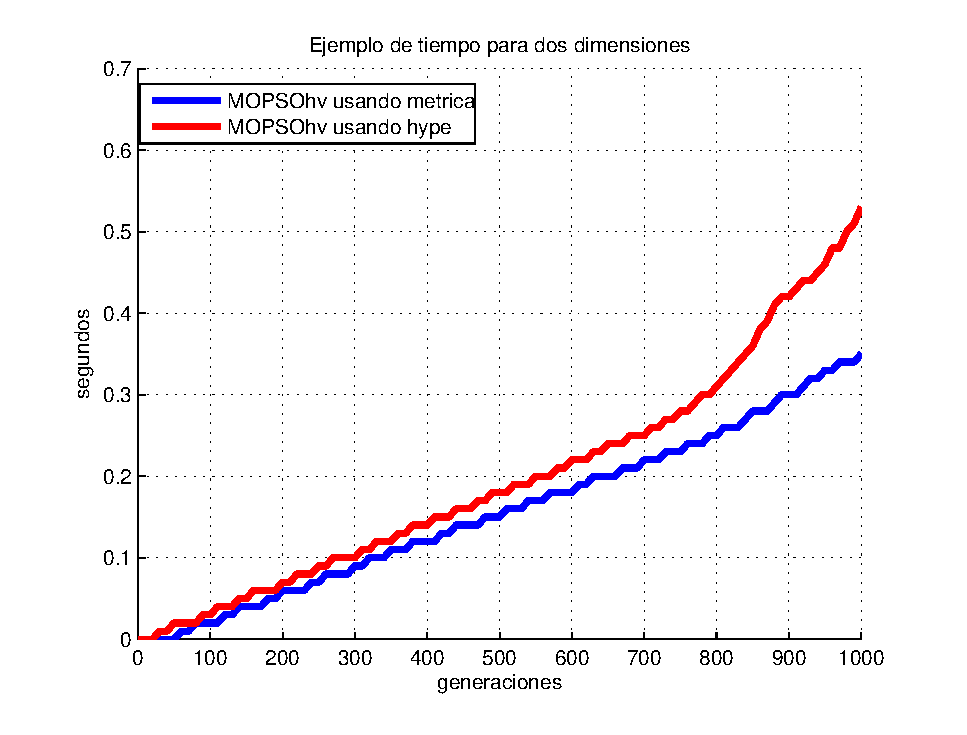
\includegraphics[scale=0.5]{Cap3/time1.eps}
    \caption[Tiempo entre MOPSOhv en dos dimensiones (a)]{Tiempo requerido en dos objetivos por el algoritmo \ref{alg:MOPSOhv} usando la 
    m\'etrica completa y el algoritmo Hype en las primeras mil generaciones.}
    \label{fig:time1}
  \end{minipage}%
  \hspace{5mm}
  \begin{minipage}{0.4\textwidth}
    \centering
    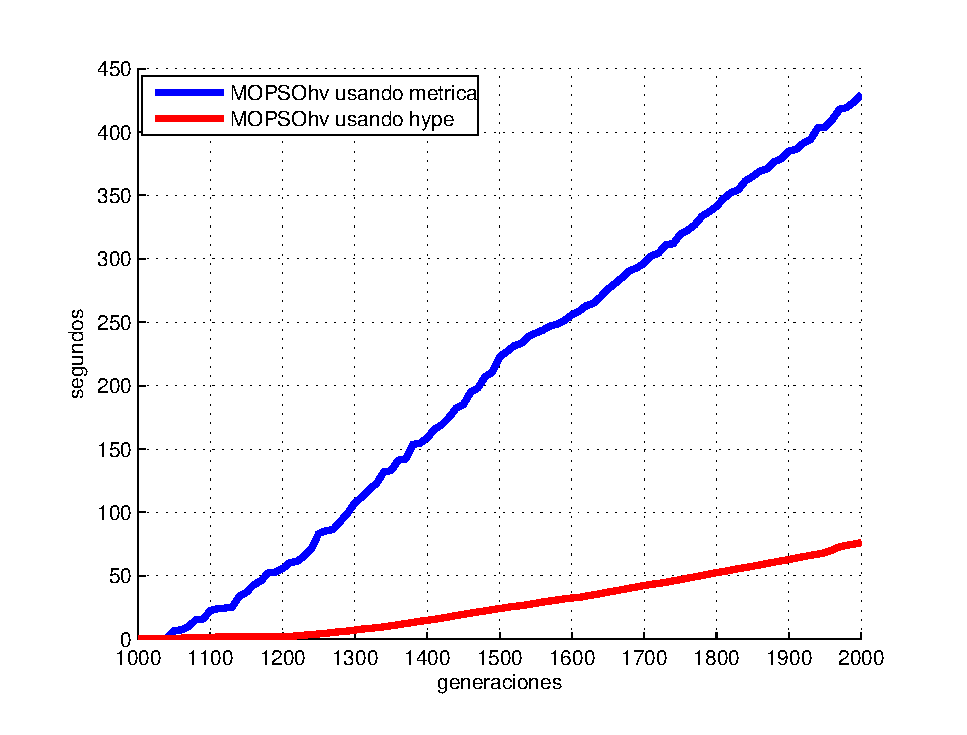
\includegraphics[scale=0.5]{Cap3/time2.eps}
    \caption[Tiempo entre MOPSOhv en dos dimensiones (b)]{Tiempo requerido en dos objetivos por el algoritmo \ref{alg:MOPSOhv} usando la 
    m\'etrica completa y el algoritmo Hype despu\'es de mil generaciones.}
    \label{fig:time2}
  \end{minipage}
  \begin{minipage}{0.4\textwidth}
    \centering
    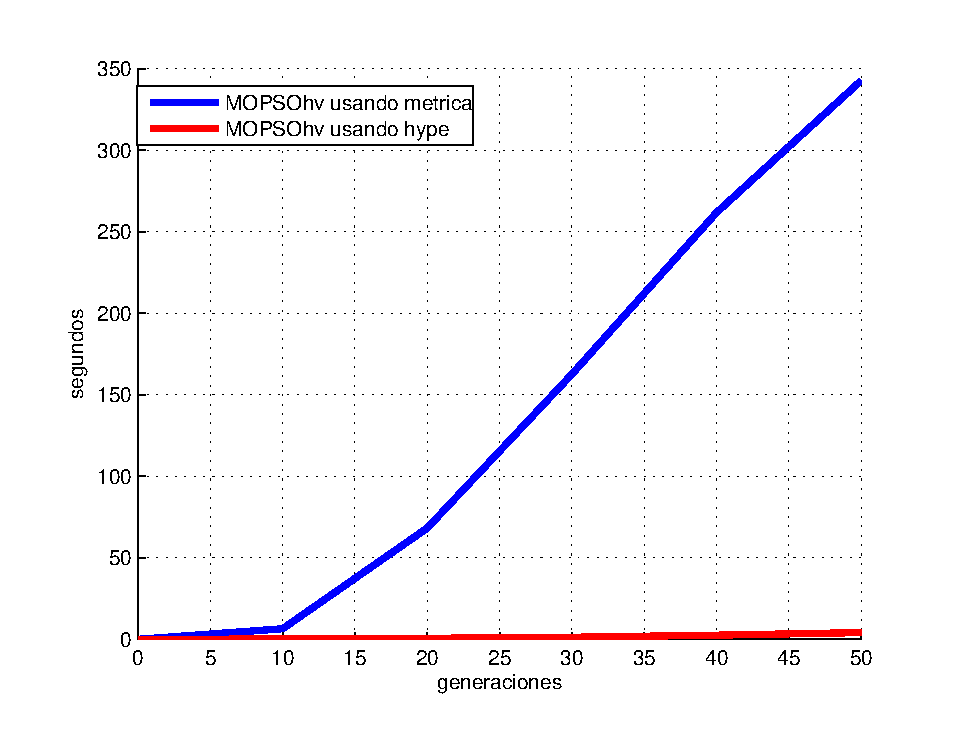
\includegraphics[scale=0.5]{Cap3/time3.eps}
    \caption[Tiempo entre MOPSOhv en tres dimensiones]{Tiempo requerido en tres objetivos por el algoritmo \ref{alg:MOPSOhv} usando la 
    m\'etrica completa y el algoritmo Hype en las primeras 50 generaciones.}
    \label{fig:time3}
  \end{minipage}%
\end{figure}
     
      
     \begin{algorithm}
    \begin{algorithmic}[1]
	\IF {$dim < 3$}
	\STATE $hypeExact(C, tam_A, ref, 1, S)$
	\ELSE
	\STATE $m = 10000$        
	\STATE $hypeSampling(C, tam_A, 0, ^{\max}\left\{ref\right\}, m, 1, S)$
	\ENDIF
	\RETURN $C$.
	\end{algorithmic}
	\caption{Calcular la contribuci\'on de las part\'iculas de la poblaci\'on}
	\label{alg:contMOPSOhv}
	\end{algorithm}
         
      \item Ordenar a la poblaci\'on en el archivo $A$ de manera descendiente conforme a su contribuci\'on al hipervolumen.
      
      \item Encontrar la part\'icula $w$, cuyo valor es el que menos contribuye al hipervolumen.
      \end{itemize}
      
\begin{enumerate}
  \item Para cada part\'icula $i$ del c\'umulo $S$, se hace lo siguiente: \\
    
    Actualizar la  velocidad y la posici\'on.
    
    \begin{itemize}
             
      \item Seleccionar aleatoriamente el mejor gu\'ia global ($gBest$) para la part\'icula $\mathcal{P}_i$ de un porcentaje $p$
      de las mejores part\'iculas de la poblaci\'on secundaria, la cu\'al es ordenada de manera descendente confome a su 
      contribuci\'on al hipervolumen (en nuestro caso, $p=0.01$ del porcentaje de la poblaci\'on secundaria actual). 
      En la figura \ref{fig:ordenado} se muestra un ejemplo de c\'omo ordenar la poblaci\'on del archivo de manera descendente 
      conforme a su contribuci\'on al hipervolumen. 

      \begin{figure}
      \begin{center}
	  \includegraphics[scale=0.8]{Cap3/1-15.eps}
      \end{center}
	\caption[Ejemplo de soluciones no dominadas ordenadas]{Un conjuto de soluciones no dominadas ordenadas de manera 
	descendente conforme a su contribuci\'on al hipervolumen.}
      \label{fig:ordenado}
      \end{figure}
      
      \item Actualizar velocidad. 
      
      Se utiliza la ecuaci\'on (\ref{equ:velocity}) (ver p\'agina \pageref{equ:velocity}) 
      para actualizar la velocidad de cada part\'icula $i$ del c\'umulo $S$. Para acelerar la convergencia 
      se hace uso de un factor de inercia $\omega = 0.4$, por tanto, la ecuaci\'on utilizada es la
      (\ref{equ:inercia}) (ver p\'agina \pageref{equ:inercia}). Finalmente, la ecuaci\'on queda de la siguiente 
      manera:	
      
       \[v^{t+1}_{i,k} = \omega \cdot v^t_{i,k} + \phi_1 \cdot rnd_1 \cdot \left(pBest^t_i - S^t_{i,k} \right) 
					    + \phi_2 \cdot rnd_2 \cdot \left(gBest - S^t_{i,k} \right),\]
      
      donde $\phi_1 = \phi_2 = 1$, $rnd_1 = Random(0, 1)$ y $rnd_2 = Random(0, 1)$. Cada part\'icula es evaluada 
      en cada objetivo $k$.
      
      \item Actualizar posici\'on. 
      
      Se utiliza la ecuaci\'on (\ref{equ:position}) (ver p\'agina \pageref{equ:position})
      para actualizar la posici\'on de cada part\'icula $i$ en cada objetivo $k$. La ecuaci\'on queda de la siguiente 
      manera:
      
      \[S^{t+1}_{i,k}=S^{t}_{i,k}+v^{t+1}_{i,k}\]
      
      \item Si la part\'icula $i$ se sale de la regi\'on de b\'usqueda, entonces, hay que reintegrarla utilizando los 
      l\'imites de b\'usqueda correspondientes al problema. Se multiplica la velocidad de la part\'icula $i$ por $-1$ 
      para cambiar la direcci\'on de b\'usqueda.  
      
      \item La mutaci\'on es una parte importante para favorecer la explotaci\'on del espacio de b\'usqueda.
      Se aplica el factor de turbulencia si se cumple que $t$ es menor a $max_{Gen} \cdot pMuta$.

    El algoritmo de c\'umulos de part\'iculas tiene una alta velocidad de convergencia. Sin embargo, esta elevada
    velocidad de convergencia puede ser perjudicial en el contexto de optimizaci\'on multi-objetivo, debido
    a que puede convergerse a un falso frente de Pareto (es decir, el equivalente de un \'optimo local en la 
    optimizaci\'on global). Para ello, introdujimos el operador de mutaci\'on que se muentra en el algoritmo \ref{alg:muta} 
    \cite{Coello04}.

    \begin{algorithm}
      \begin{algorithmic}[1]			
	\REQUIRE  Part\'icula $S_i$ para mutar, $dim$ el n\'umero de dimensiones, $max_{Gen}$ el n\'umero m\'aximo de generaciones,
	      $pMuta$ la probabilidad de mutaci\'on y $t$ la generaci\'on actual.
	\ENSURE Part\'icula $S_i$ mutada.
	\IF {$flip \left( \left( 1 - t / max_{Gen}  \right)^{5/pMuta} \right) $}
	  \STATE $wdim = random(0, dim-1)$
	  \STATE $rango = \left(u_{wdim} - l_{wdim}\right)\cdot \left(1 - t/max_{Gen} \right)^{5/pMuta}$
	  \STATE $ub = S_{i,wdim} + rango$
	  \STATE $lb = S_{i,wdim} + rango$
	  \IF{$lb < l_{wdim}$}
	    \STATE $lb = l_{wdim}$
	  \ENDIF
	  \IF{$ub > u_{wdim}$}
	    \STATE $ub = u_{wdim}$
	  \ENDIF
	  \STATE $S_{i,wdim} = random\left(lb,ub\right)$
	\ENDIF	
	\RETURN $S_i$
  \end{algorithmic}
  \caption{Operador de Mutaci\'on}
  \label{alg:muta}
  \end{algorithm}

  \end{itemize}
  
  \item Evaluar todas las part\'iculas de la poblaci\'on $S^t$. Se eval\'uan los valores de 
     todas las part\'iculas $i$ en cada funci\'on objetivo $k$. 
      
      \[p^t_{i,k} = F \left(S^t_{i,k} \right)\] 
    
  \item Actualizar las soluciones no dominadas en $A^t$. 
  
  \begin{itemize}
   \item Se insertan todas las soluciones no dominadas de $S^t$ en $A^t$, s\'olo si las soluciones no son 
  dominadas por alguna ya almacenada. Todas las soluciones dominadas por la nueva soluci\'on son eliminadas del archivo. 
  
  \item Si el archivo $A$ ya est\'a lleno, es decir, $nd > tam_A$. Las soluciones son reemplazadas conforme al siguiente criterio: 
  se hace uso del algoritmo \ref{alg:hvaprox} que aproxima la contribuci\'on (de la misma forma que el paso $3$). Se reemplaza la 
  part\'icula $w$, que es la que menos contribuye, con la nueva part\'icula. Se calcula la contribuci\'on y
  se encuentra otra vez a la part\'icula $w$.
  
  \end{itemize}
  
  \item Actualizar el $pBest$ de cada part\'icula $i$ en cada dimensi\'on $k$. 
  
  Una forma de realizarlo es si el actual $pBest_i$ es mejor que el almacenado en memoria, entonces se actualiza el $pBest^t$, de la siguiente 
  manera:
  
  \[pBest^t_{i,k} = S^t_{i,k}\]
  
  Siguiendo esta topolog\'ia no se tiene una buena interacci\'on con las dem\'as part\'iculas para generar buenas soluciones. 
  Por lo tanto, se decidi\'o actualizar el $pBest^t$ utilizando la poblaci\'on secundaria (sin considear el porcentaje $p$ de 
  las mejores   part\'iculas de esta poblaci\'on), es decir, solo se comparte informaci\'on de un porcentaje $r$ de part\'iculas 
  que pertenecen a las mejores soluciones generadas hasta el momento, las cuales ser\'an utlizadas en el entorno social del 
  algoritmo (para nuestro caso $r=1$). El $pBest^t$ se actualiza de acuerdo al algoritmo \ref{alg:contpBest}.
  
  \begin{algorithm}
    \begin{algorithmic}[1]
	\STATE $nttop = ((tam_A - 1) \cdot r)$
	\STATE $top = ((tam_A - 1) \cdot p)$
	\FOR {cada part\'icula $i$ hasta $tam_S$}	  
	  \STATE $j= RandomInt(top+1,nttop)$
	  \STATE $pBest^t_i = A^t_j$
	\ENDFOR
	\RETURN $pBest^t$.
	\end{algorithmic}
	\caption{Actualizar $pBest^t$}
	\label{alg:contpBest}
	\end{algorithm}
  
  \item Incrementar el contador de generaciones en uno.
  
  \[t= t + 1\]
  
  \item Si no se cumple el criterio de paro, retornar al paso $3$.
  
\end{enumerate}

\item Retornar al c\'umulo con la aproximaci\'on al frente de Pareto.

\end{enumerate}
\rule{\linewidth}{1pt}



\chapter{Evaluaci\'on del algoritmo propuesto y resultados}

En este cap\'itulo se presenta la evaluaci\'on experimental del algoritmo desarrollado en este trabajo de tesis. 
La evaluaci\'on se realiz\'o utilizando un conjunto diverso de problemas multi-objetivo que reunen diferentes caracter\'isticas que causan 
dificultades a un algoritmo evolutivo multi-objetivo. El estudio experimental descrito en este cap\'itulo est\'a dividido 
en tres partes: la primera parte muestra los resultados para el conjunto de problemas ZDT (\textit{Zitzler-Deb-Thiele}), 
la segunda muestra los resultados para el conjunto de problemas de DTLZ (\textit{deb-Thiele-Laumanns-Zitzler}). 
Finalmente, la tercera y \'ultima parte muestra los resultados de escalabilidad. Los resultados se contrastan 
con las soluciones obtenidas por los algoritmos NSGA-II (\textit{the Nondominated Sorting Genetic Algoritm -II}), SMS-EMOA 
(\textit{Multi-objective Selection based on Dominated Hypervolume}) y MOPSOcd (\textit{Multi-objective Particle Swarm Optimizer based on 
Crowding Distance}).
  
  \section*{Par\'ametros}
  
  Los par\'ametros utilizados para generar las soluciones de los algoritmos MOPSOhv y MOPSOcd se muentran en la tabla
  \ref{tab:parametros1}. Se us\'o un factor de 
  inercia $\omega = 0.4$ y constantes sociales $\varphi_{1}=\varphi_{2}=1$.
 
 \begin{table}[H]
  \begin{center}
    \begin{tabular}{|l||c|c|c|}
	\hline
	& \textbf{Generaciones}  & \textbf{Poblaci\'on} & \textbf{Mutaci\'on} \\
	\hline
	\hline
	\textbf{MOPSOhv} & 1200 & 100 &0.5\\ 
	\hline
	\textbf{MOPSOcd} & 1200 & 100 &0.5\\
	\hline
	\end{tabular}
	\caption{Par\'ametros para los algoritmos de c\'umulos de part\'iculas}
  \label{tab:parametros1}
  \end{center}
\end{table}

Los par\'ametros utilizados para generar las soluciones del NSGA-II se muestran en la tabla \ref{tab:parametros2}. Los par\'ametros
utilizados para generar las soluciones del SMS-EMOA se muestran en la tabla \ref{tab:parametros3}.

\begin{minipage}{0.5\textwidth}
\begin{table}[H]
  \begin{center}
    \begin{tabular}{|l||c|c}
	\hline
	Generaciones  & 1200 \\ 
	\hline
	Poblaci\'on & 100 \\ 
	\hline
	Cruza & 0.9 \\
	\hline
	Mutaci\'on & $\frac{1}{\vec{x}}$ \\
	\hline
  \end{tabular}
  \caption{Par\'ametros de NSGA-II}
  \label{tab:parametros2}
\end{center}
\end{table}
\end{minipage}
\begin{minipage}{0.5\textwidth}
\begin{table}[H]
	\begin{center}
		\begin{tabular}{|l||c|c}
			\hline
			Generaciones  & 1200 \\ 
			\hline
			Poblaci\'on & 100 \\ 
			\hline
			$\eta_c = \eta_m$ & 20 \\ 
			\hline
			Mutaci\'on & $\frac{1}{\vec{x}}$\\ 
			\hline			
		\end{tabular}
		\caption{Par\'ametros de SMS-EMOA}
		\label{tab:parametros3}
	\end{center}
\end{table}
\end{minipage}

El c\'odigo est\'a implementado en lenguaje C y la evaluaci\'on del conjunto diverso de problemas multi-objetivo se realizaron en una 
computadora port\'atil con las siguientes caracter\'isticas: un procesador Intel(R) Core(TM)2 Duo CPU T5800 a 2.00GHz, 4 Gb de Memoria RAM, 
un disco duro de 320 Gb y un sistema operativo Ubuntu 12.04.1 LTS de 64 bits.

El uso de una sola m\'etrica dif\'icilmente puede reflejar el desempe\~no global de un algoritmo evolutivo multi-objetivo. Algunas
m\'etricas miden la convergencia del algoritmo al frente de Pareto real, otras la distribuci\'on y la diversidad de las soluciones. 
En este caso necesitamos evaluarlo considerando varias m\'etricas simult\'aneamente. Sin embargo, la m\'etricas evalu\'an dos 
objetivos en conflicto (la convergencia y la diversidad). Si los valores de las m\'etricas de un algoritmo dominan a las de otro,
entonces podemos afirmar que el primero es mejor que el segundo. En otro caso, no podemos concluir nada acerca de los dos algoritmos.
Las m\'etricas que se utilizar\'an para evaluar la eficacia son el espaciamiento para evaluar la distribuci\'on; y la distancia generacional 
invertida, la cobertura de dos conjuntos y el indicador del hipervolumen para evaluar la convergencia. La definici\'on formal de las m\'etricas 
utilizadas se muestran en la secci\'on \ref{sec:metric} en la p\'agina \pageref{sec:metric}.

\newpage
\section{Conjunto de problemas ZDT}

Estos problemas est\'an dise\~nados poniendo \'enfasis en algunas de las caracter\'isticas que causan dificultades para un algoritmo 
evolutivo multi-objetivo. Estos problemas tienen una misma estructura y consisten de tres funciones, $F$, $g$ y $h$, se describe a 
continuaci\'on \cite{Zitzler2000}:

\begin{align*}
\text{Minimizar}\hspace{0.5cm} F&=(f_1(x_1),f_2(x_2))\\
\text{Sujeto a }\hspace{0.5cm} f_2(x)&=g(x_2,\ldots,x_m)\cdot h(f_1(x_1),g(x_2,\ldots,x_m)),\\
\text{donde}\hspace{0.5cm} x&= (x_1,\ldots, x_m)
\end{align*}

La funcion $f_1$ depende solamente de la primera variable de decisi\'on, $g$ es una funci\'on de las
$m-1$ variables restantes, y los par\'ametros de $h$ son los valores de las funciones $f_1$ y $g$.

\begin{itemize}
 
\item La funci\'on de prueba \textbf{ZDT1} tiene un frente de Pareto convexo:
\begin{align*}
f_1(x)&=x_1\\
f_2(x,g(x))&=g(x)\cdot\left(1-\sqrt{ \frac{f_1}{g(x)}}\right)\\
g(x)&=1+\frac{9}{n-1}\cdot\sum_{i=2}^nx_i
\end{align*}
donde $n=30$ y $x_i\in[0,1]$ con $i=1,\ldots, n$. El frente de Pareto real se forma con $g(x)=1$ (figura \ref{fig:zdt1}).

\item La funci\'on de prueba \textbf{ZDT2} tiene un frente de Pareto c\'oncavo:

\begin{align*}
f_1(x)&=x_1\\
f_2(x,g(x))&=g(x)\cdot(1- \left( \frac{f_1}{g(x)}\right)^2)\\
g(x)&=1+\frac{9}{n-1}\cdot\sum_{i=2}^nx_i
\end{align*}
donde $n=30$ y $x_i\in[0,1]$ con $i=1,\ldots, n$. El frente de Pareto real se forma con $g(x)=1$ (figura \ref{fig:zdt2}).

\item La funci\'on de prueba \textbf{ZDT3} tiene un frente de Pareto discontinuo y convexo:

\begin{align*}
f_1(x)&=x_1,\\
f_2(x,g)&=g(x)\cdot\left(1-\sqrt{\frac{f_1(x)}{g(x)}}-\frac{f_1(x)}{g(x)}\sin(10\cdot\pi\cdot f_1(x))\right)\\
g(x)&=1+\frac{9}{n-1}\cdot\sum_{i=2}^nx_i
\end{align*}
donde $n=30$ y $x_i\in[0,1]$ con $i=1,\ldots, n$. El frente de Pareto real se forma con $g(x)=1$. La funci\'on seno
en $h$ produce una discontinuidad en el frente de Pareto. Sin embargo, no hay discontinuidad en el espacio de las variables 
de decisi\'on (figura \ref{fig:zdt3}).

\item La funci\'on de prueba \textbf{ZDT4} tiene $21^9$ frentes locales, lo que pone a prueba la habilidad de un 
algoritmo para lidiar con problemas multifrontales:

\begin{align*}
f_1(x)&=x_1,\\
f_2(x,g(x))&=g(x)\cdot \left(1-\sqrt{ \frac{f_1(x)}{g(x)}}\right),\\
g(x)&=1+10\cdot(n-1)+ \sum_{i=2}^n(x_i^2-10\cdot \cos(4\cdot\pi\cdot x_i))
\end{align*}

donde $n=10$, $x_1\in[0,1]$ y $x_i \in[-5,5] $ con $i=2, \ldots, n$. El frente de Pareto real se forma con $g(x)=1$ (figura \ref{fig:zdt4}).

\item La funci\'on de prueba \textbf{ZDT6} tiene un espacio de b\'usqueda no uniforme:

\begin{align*}
f_1(x)&=1- e^{(-4\cdot x_1)} \cdot \sin^6(6\cdot\pi\cdot x_1),\\
f_2(x,g(x))&=g(x)\cdot(1-\left(\frac{f_1}{g(x)}\right)^2),\\
g(x)&=1+9\cdot\left[\frac{\sum_{i=2}^n}{9}\right]^{0.25}
\end{align*}

donde $n=10$, $x_1\in[0,1]$ y $x_i \in[-5,5]$ con $i= 2, \ldots, n$. El frente de Pareto real se forma con $g(x)=1$.
Este problema tiene una baja densidad en las soluciones cerca del frente de Pareto real y una alta densidad lejos del mismo (figura \ref{fig:zdt6}).

\end{itemize}

\begin{figure}
\centering
    \centering
    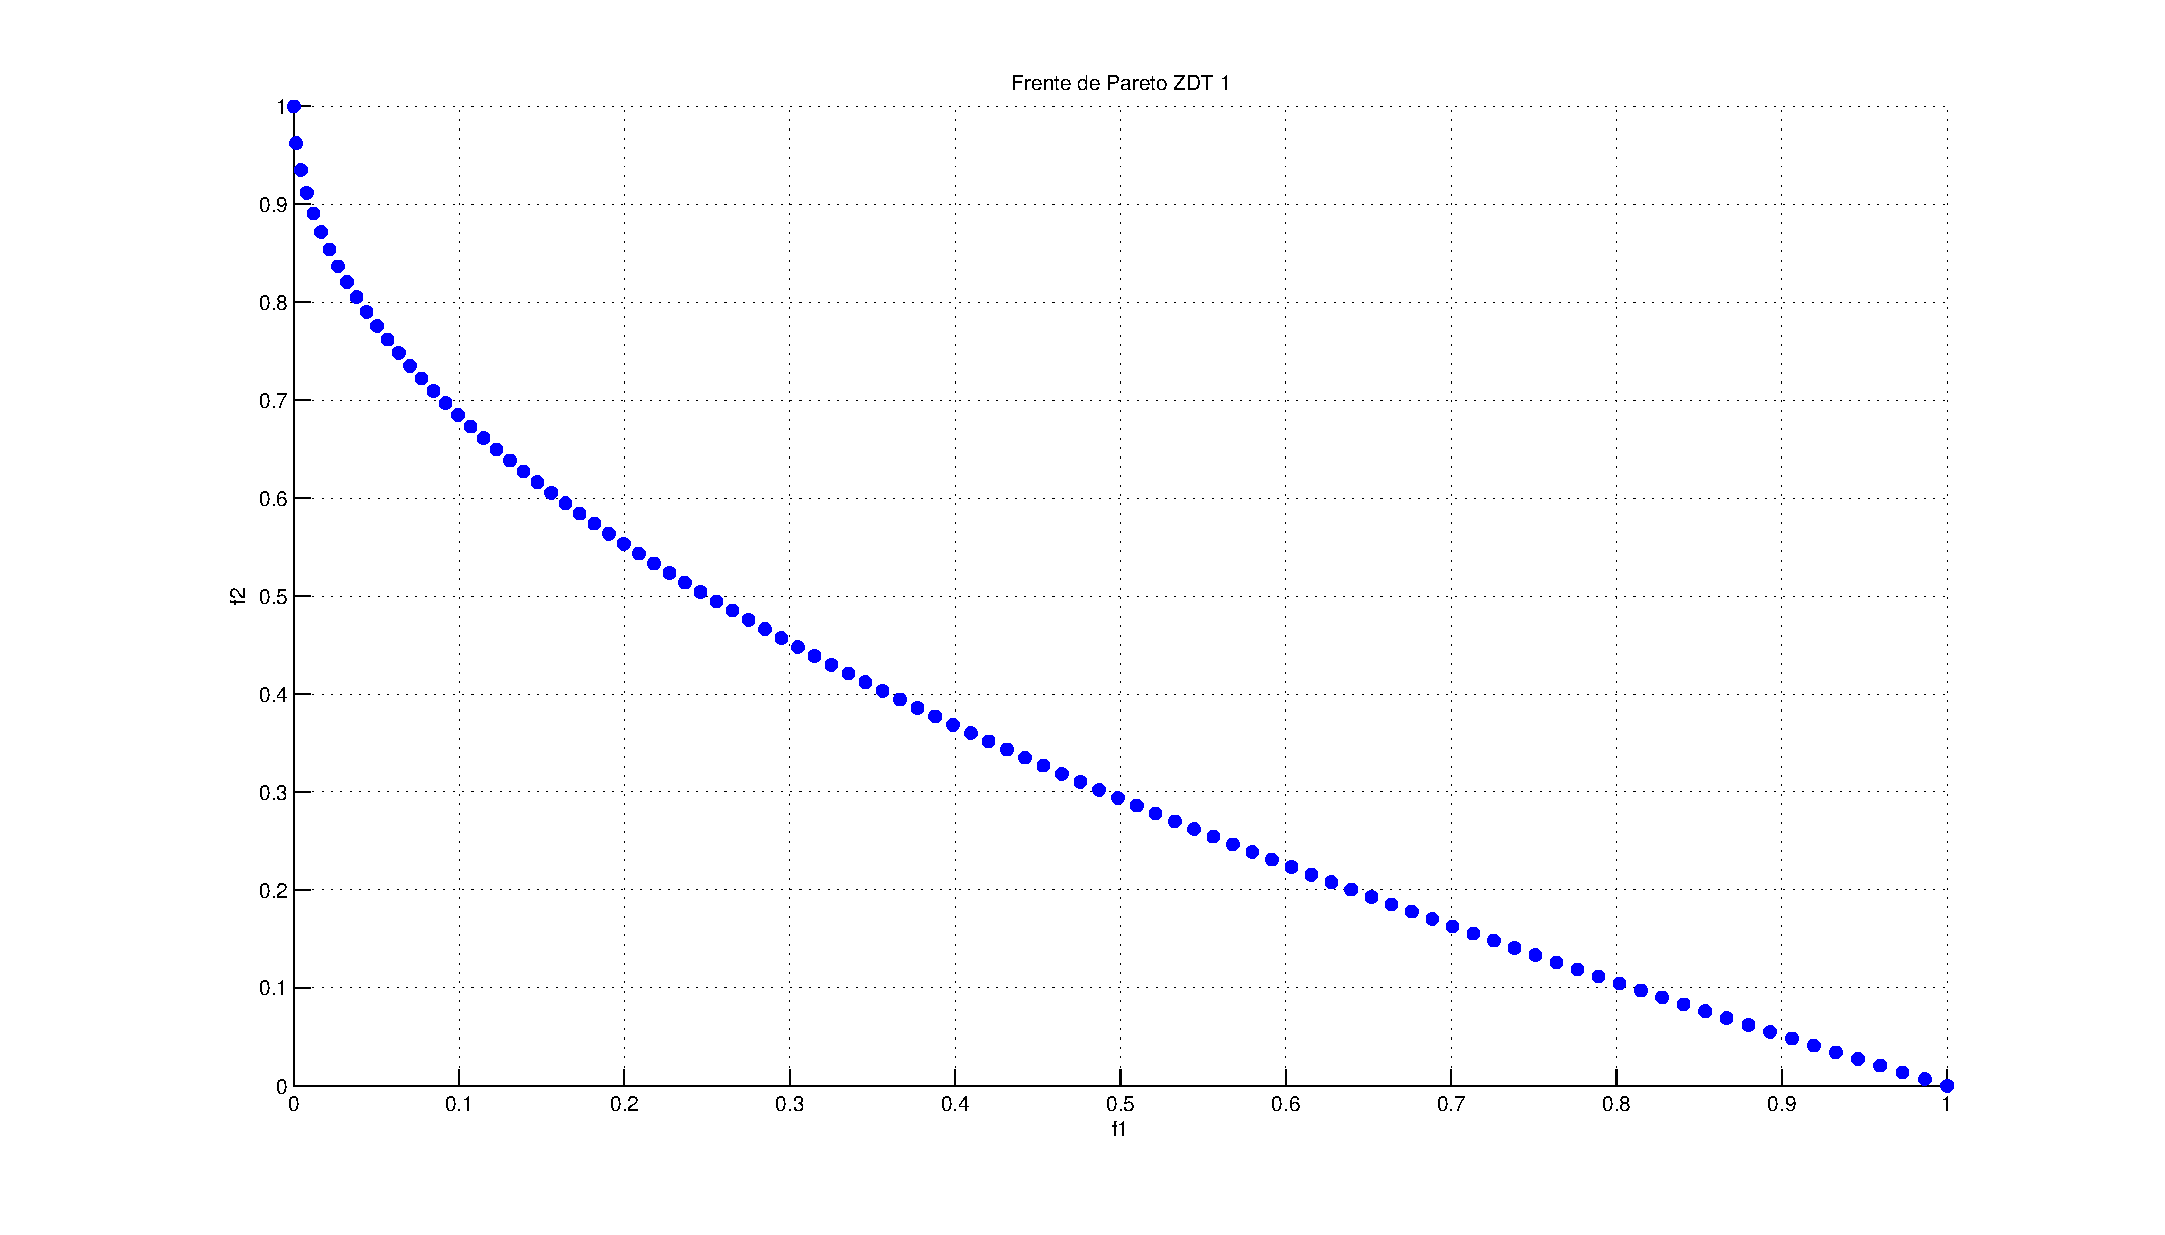
\includegraphics[scale=0.4]{ApendiceA/paretoZDT1.eps}
    \caption{Frente de Pareto verdadero de ZDT1}
    \label{fig:zdt1}
\end{figure}
 
\begin{figure}
\centering
 
    \centering
    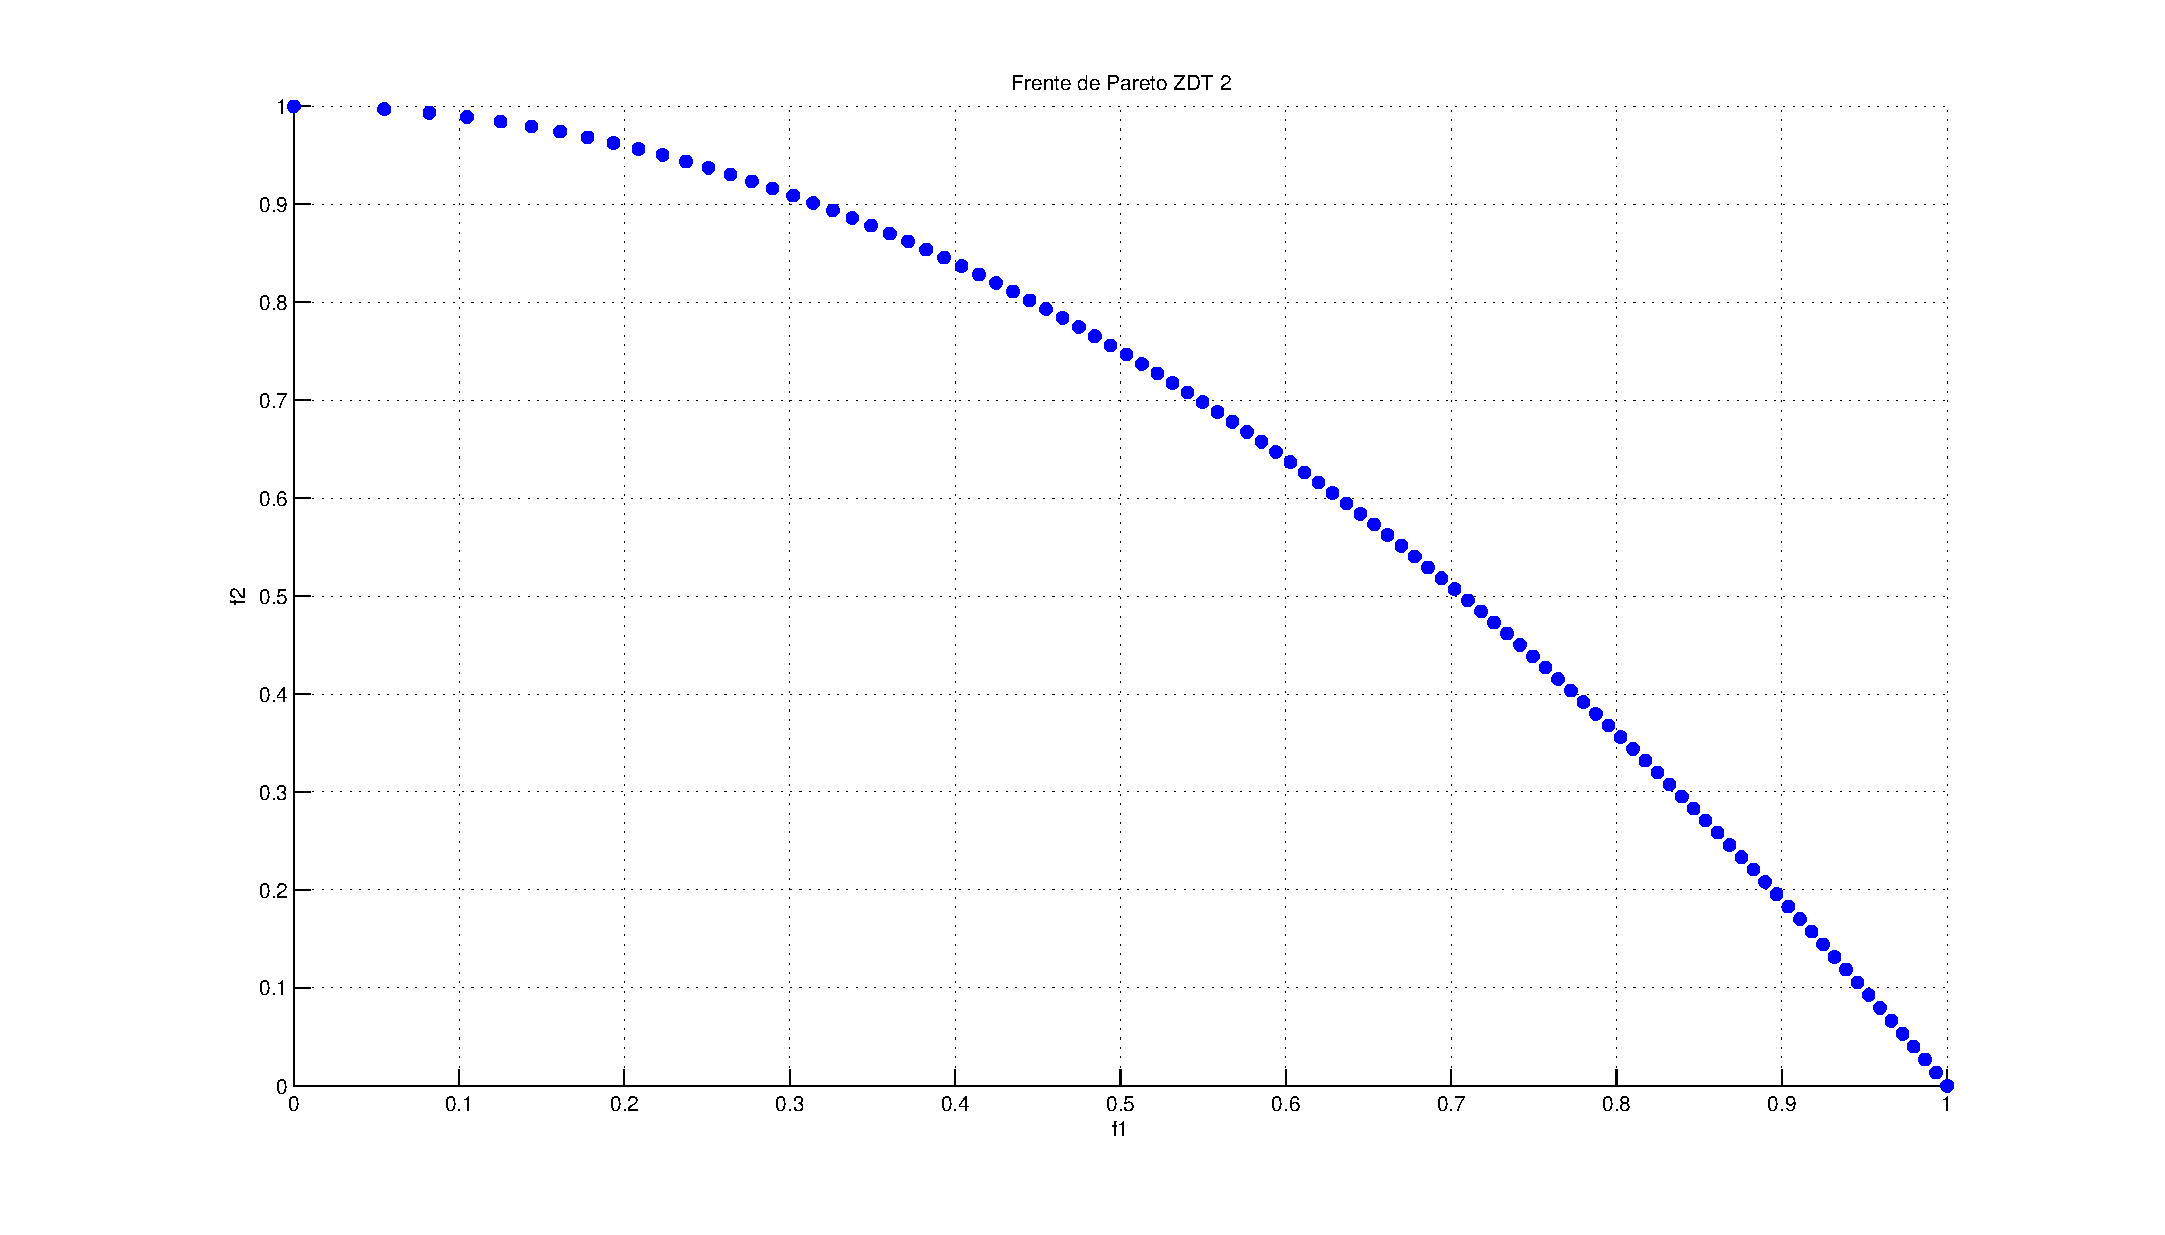
\includegraphics[scale=0.4]{ApendiceA/paretoZDT2.eps}
    \caption{Frente de Pareto verdadero de ZDT2}
    \label{fig:zdt2}
\end{figure}

\begin{figure}
\centering
    \centering
    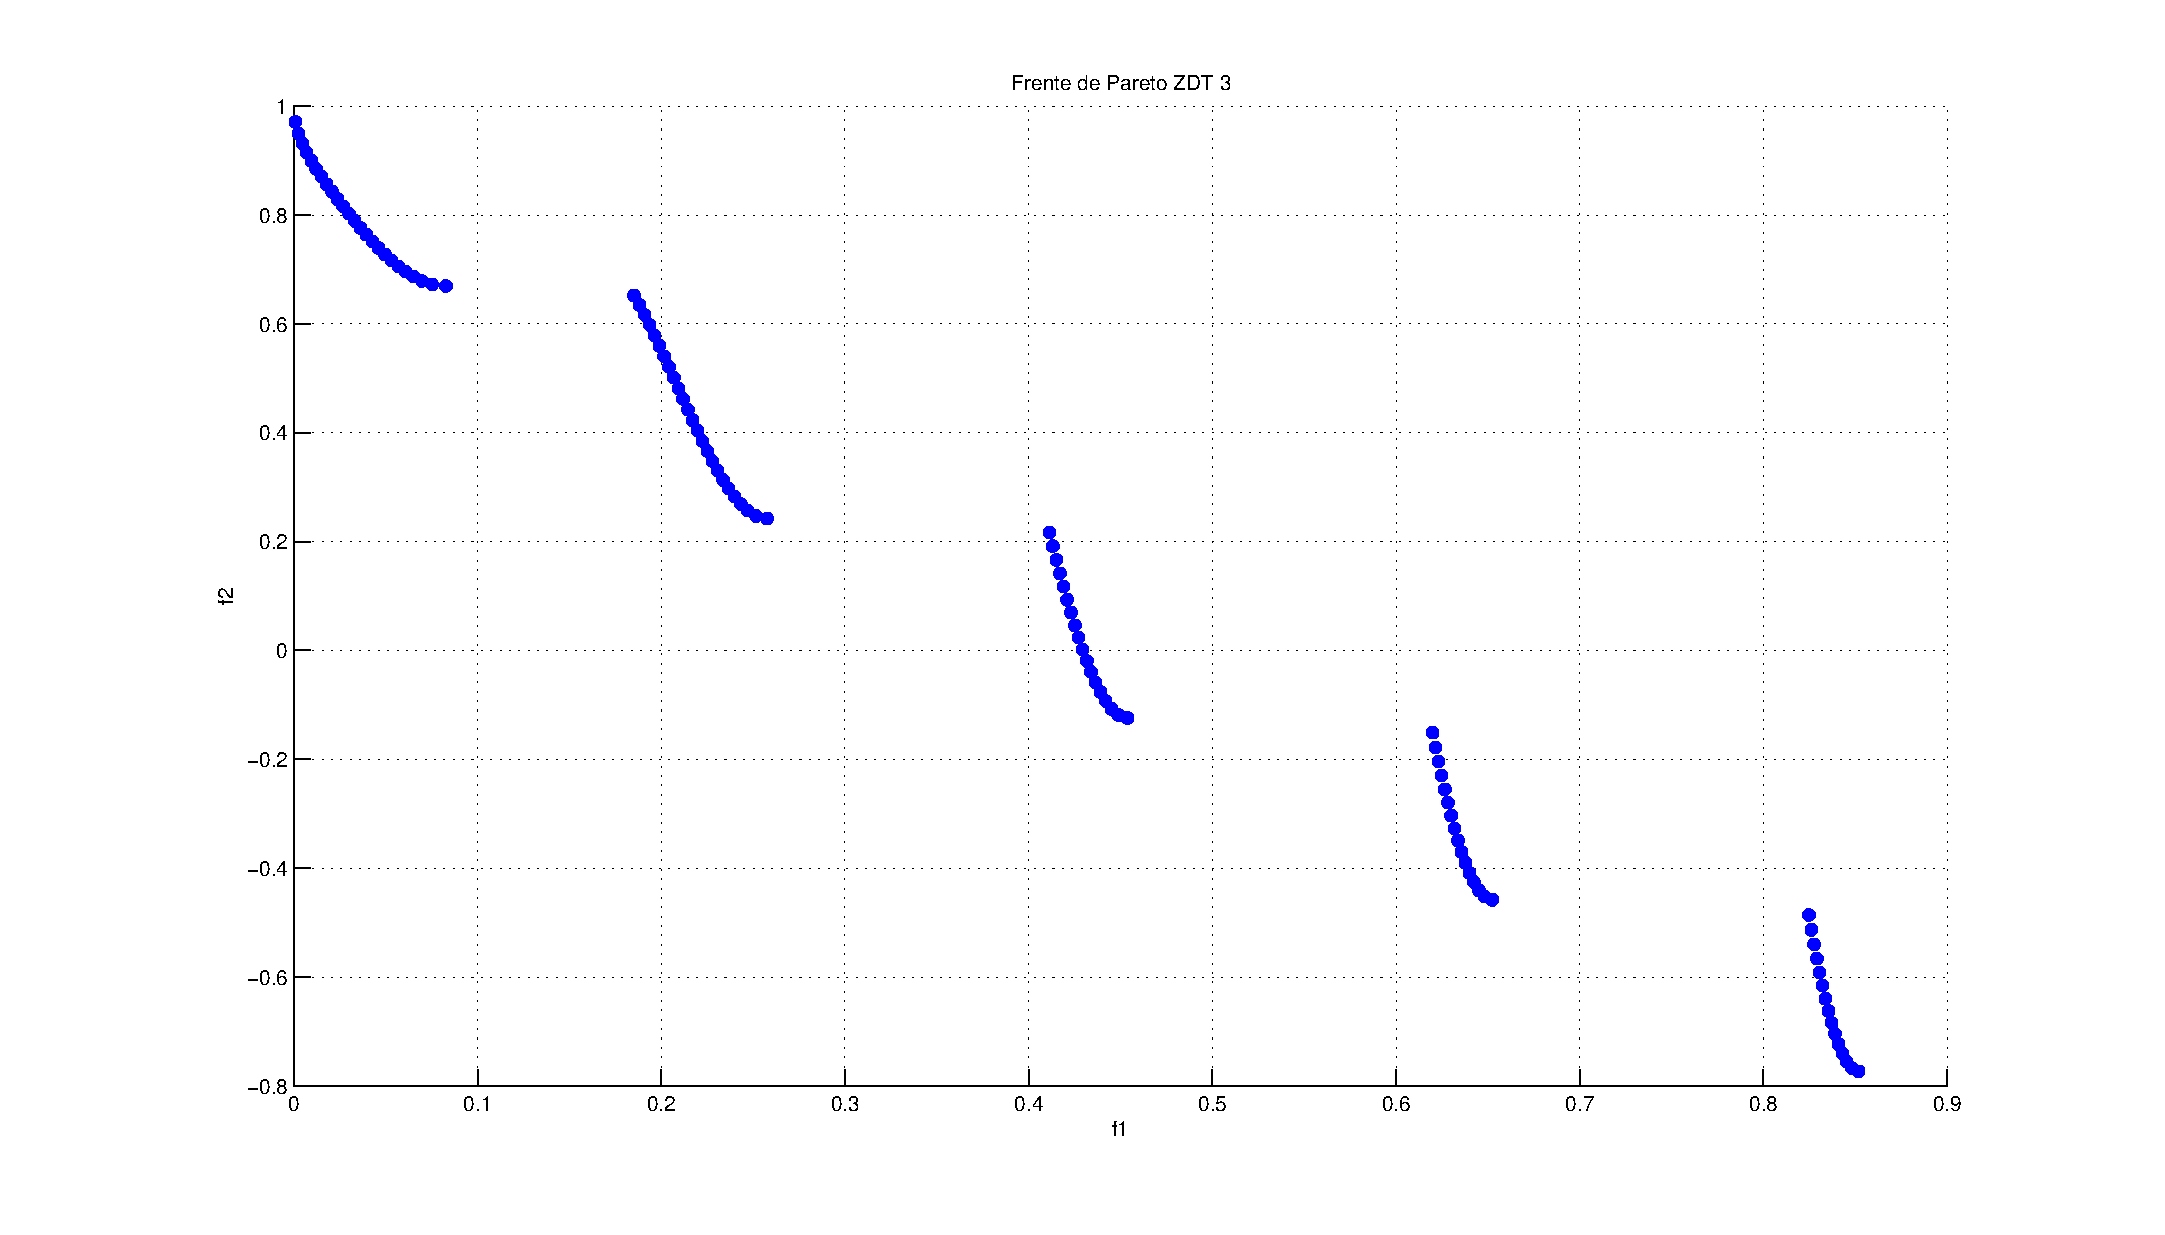
\includegraphics[scale=0.4]{ApendiceA/paretoZDT3.eps}
    \caption{Frente de Pareto verdadero de ZDT3}
    \label{fig:zdt3}
\end{figure}

\begin{figure}
\centering
    \centering
    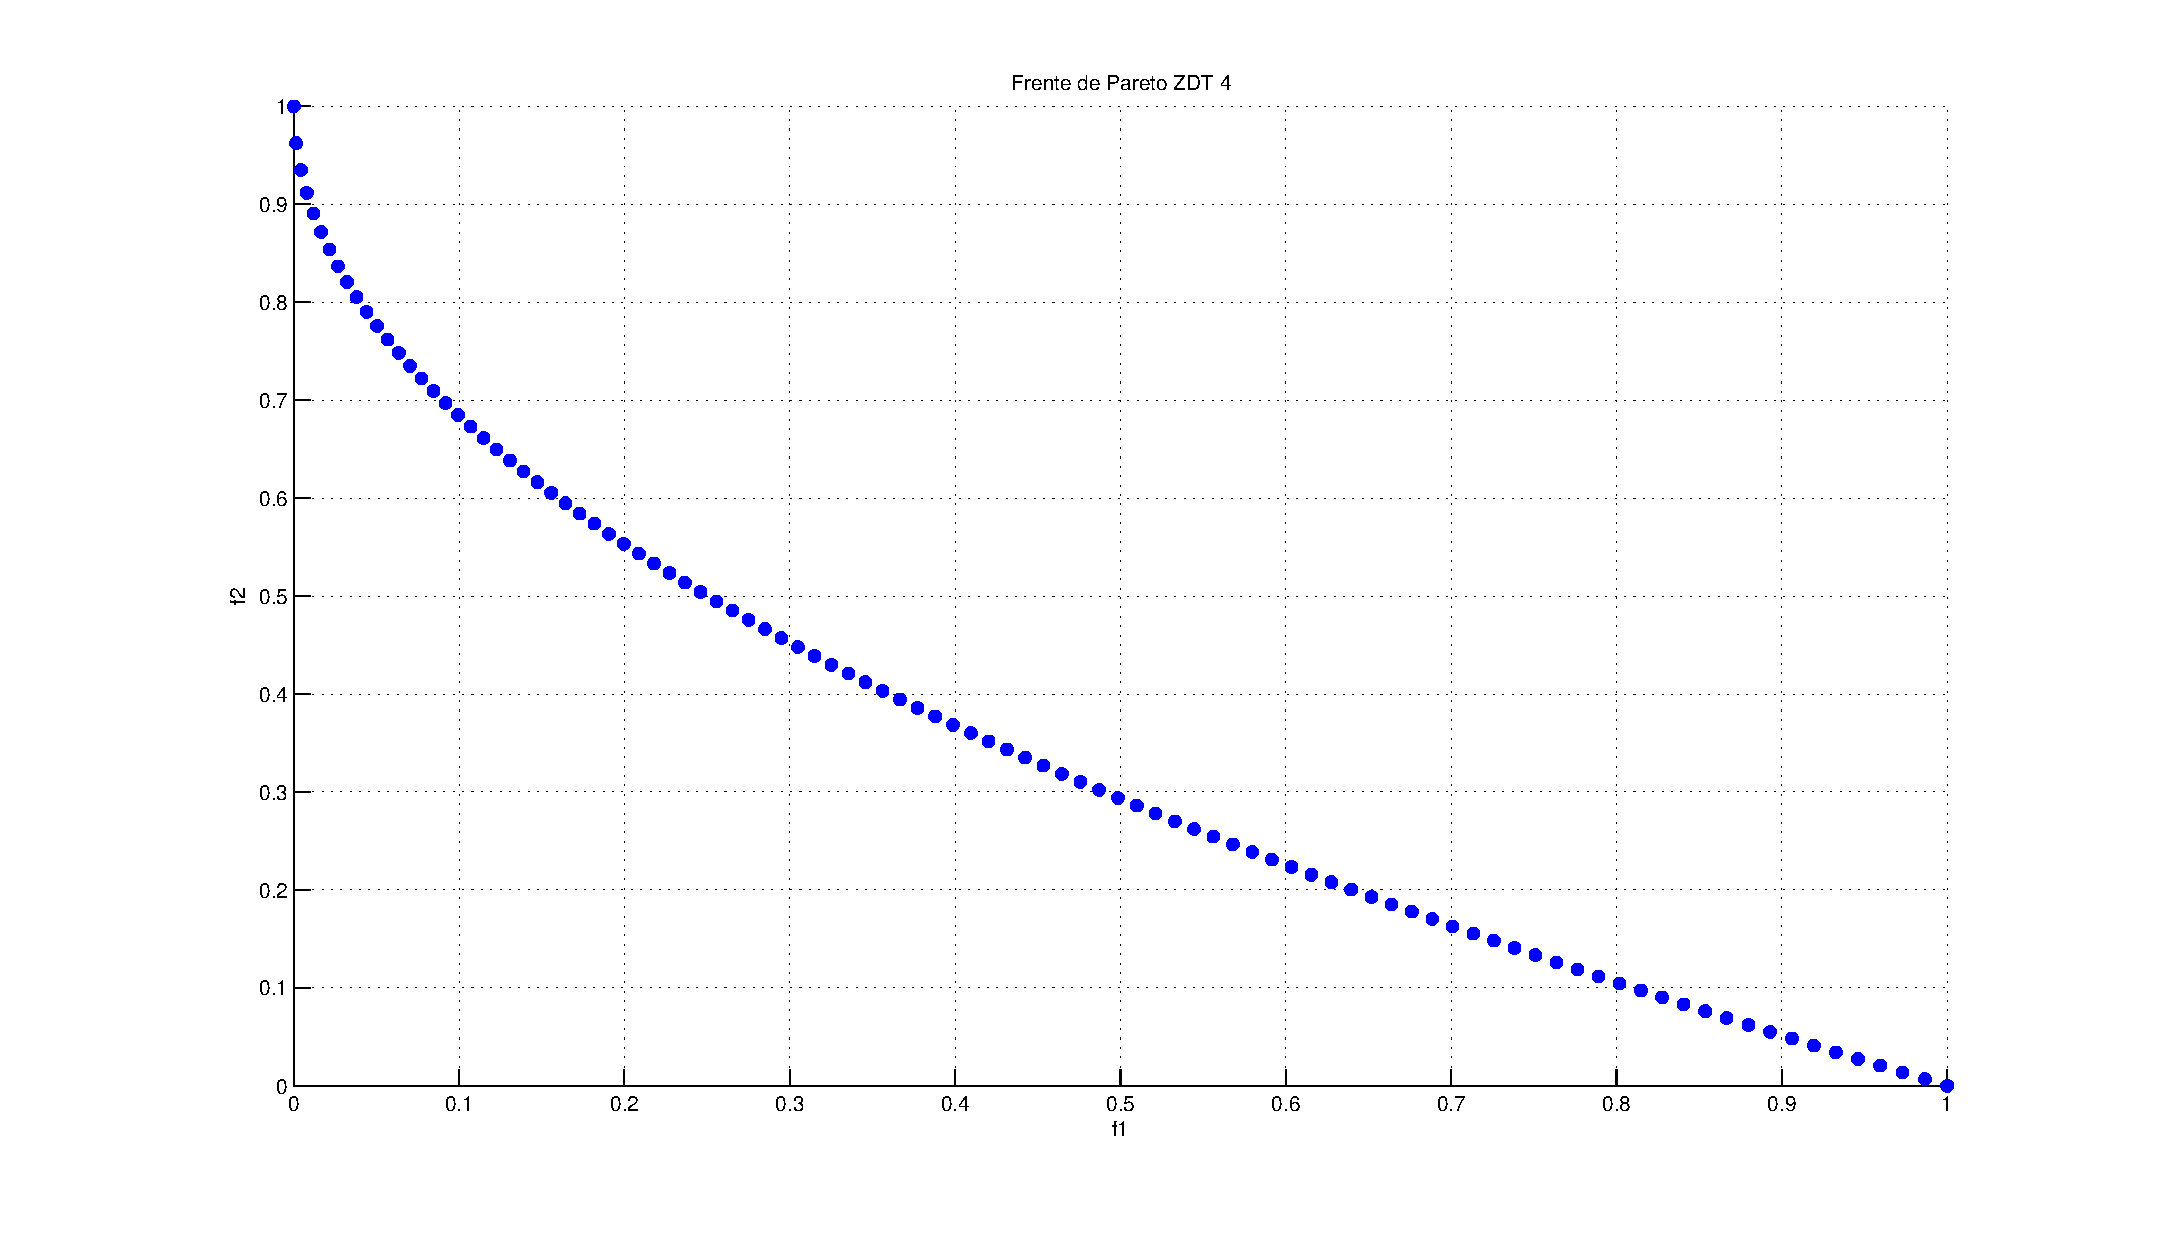
\includegraphics[scale=0.4]{ApendiceA/paretoZDT4.eps}
    \caption{Frente de Pareto verdadero de ZDT4}
    \label{fig:zdt4}
\end{figure}
\begin{figure}
\centering
    \centering
    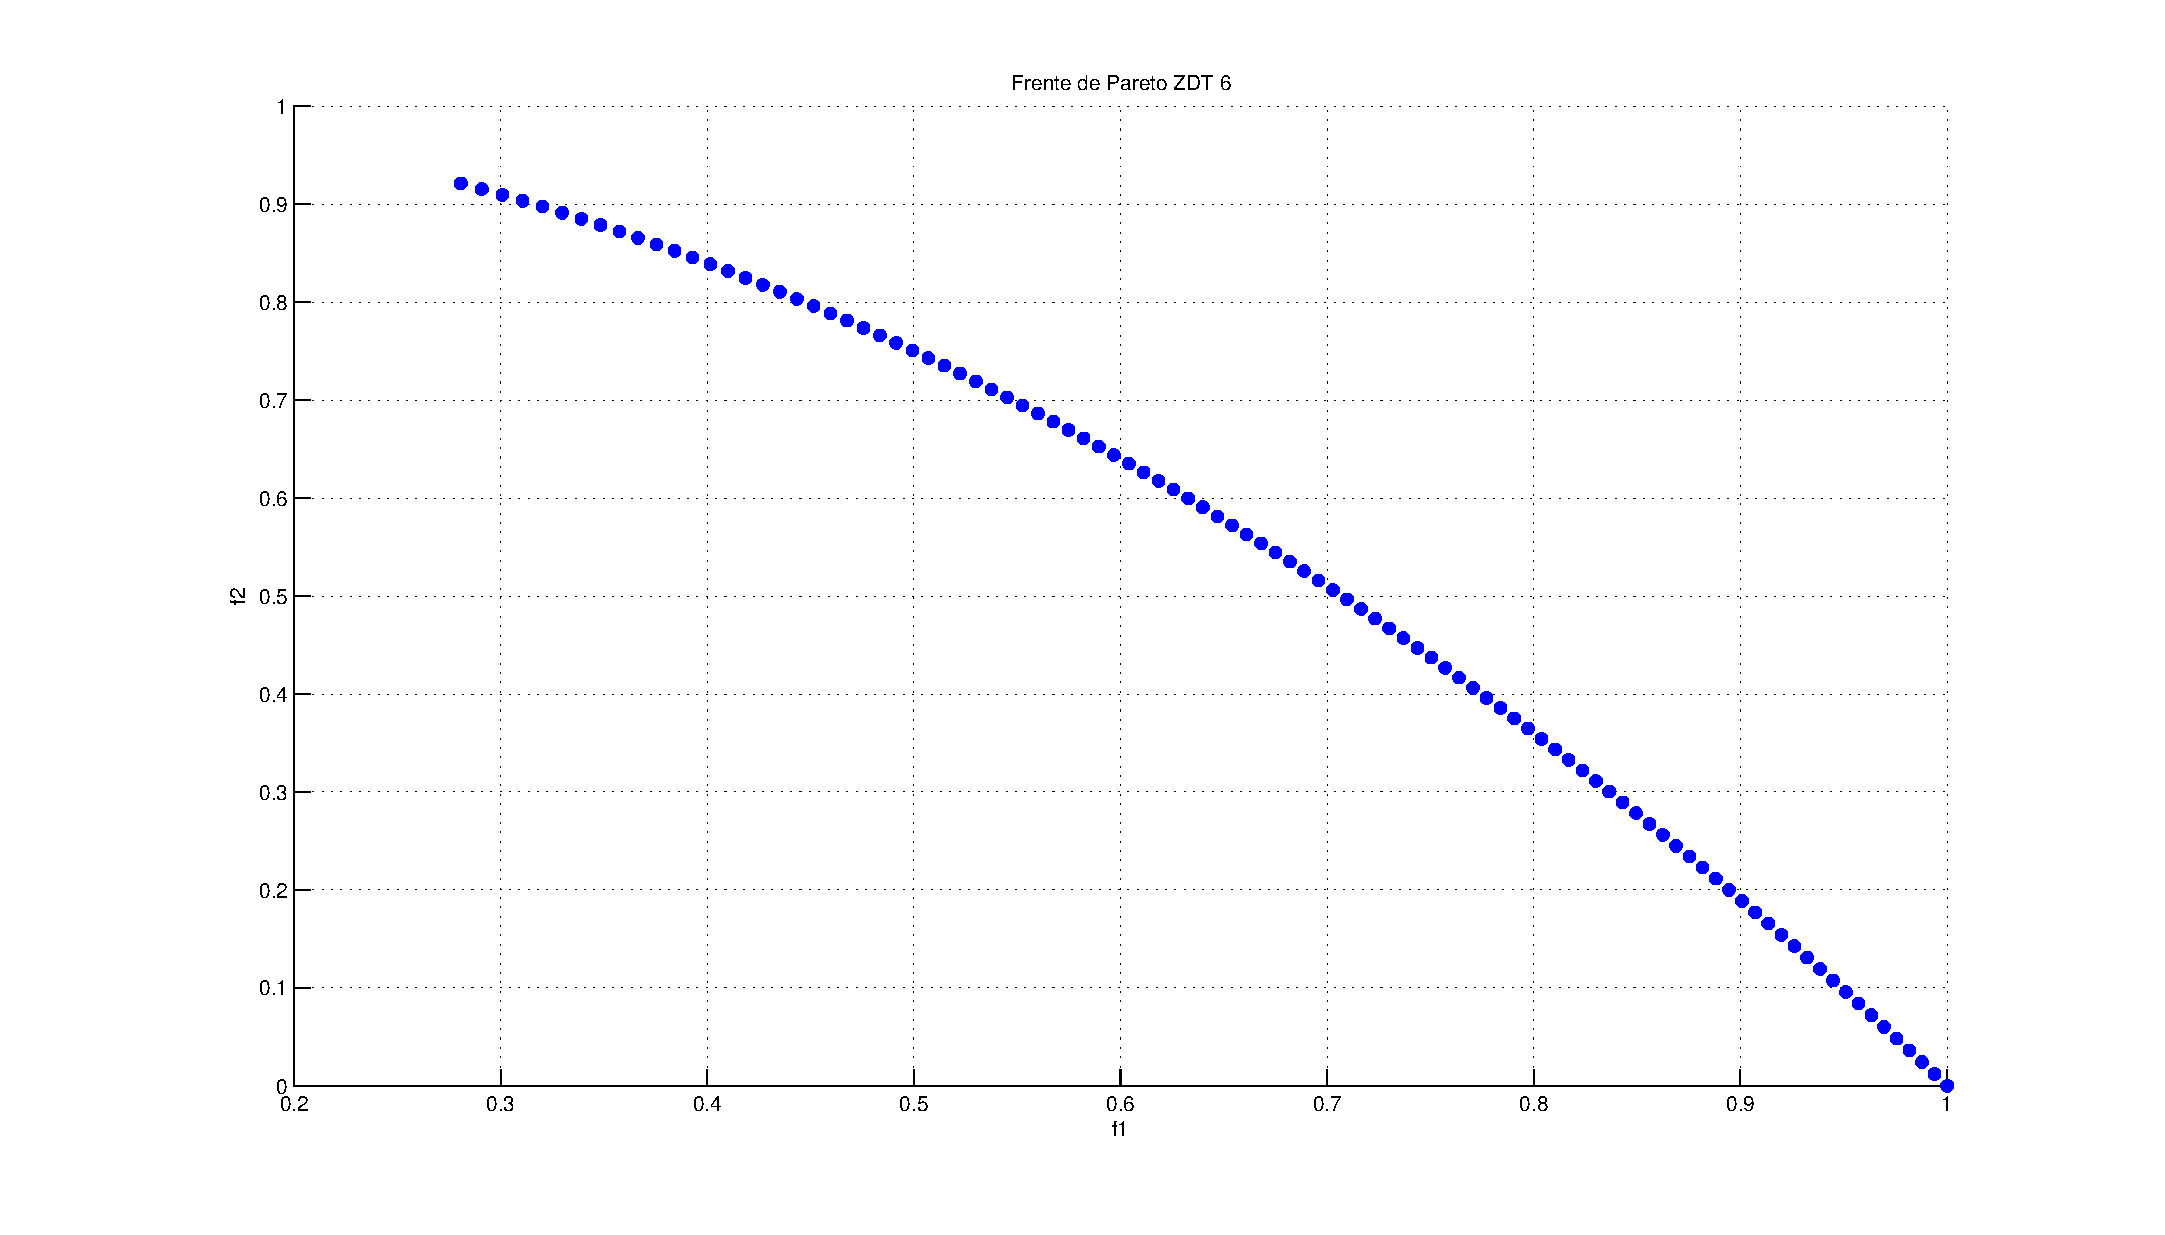
\includegraphics[scale=0.4]{ApendiceA/paretoZDT6.eps}
    \caption{Frente de Pareto verdadero de ZDT6}
    \label{fig:zdt6}
 
\end{figure}

\newpage
\section{Evaluaci\'on del conjunto de problemas ZDT}
  La comparaci\'on de los resultados de cada algoritmo se realiz\'o con los valores promedio obtenidos por cada m\'etrica.
  El punto de referencia utilizado en cada caso para el indicador del hipervolumen se muestra en la tabla \ref{tab:ref}.
  
  Los resultados obtenidos para los primeros tres problemas ZDT son similares para a mayoria de los resultados. 
  Donde el SMS-EMOA resulta ganador en la mayor parte de las m\'etricas convergencia seguido por nuestra propuesta (MOPSOhv), 
  como se muestra en las tablas \ref{tab:zdt1}, \ref{tab:zdt2} y \ref{tab:zdt3}. Sin embargo, nuestra propuesta 
  dominada a las soluciones del NSGA-II y MOPSOcd excepto al SMS-EMOA, de acuerdo a la m\'etrica de cobertura.
  
  Conforme a estos resultados se tiene una jerarqu\'ia en orden descendente en t\'erminos de convergencia en estos primeros tres 
  problemas:

\begin{enumerate}
  \item SMS-EMOA
  \item MOPSOhv
  \item NSGA-II
  \item MOPSOcd
\end{enumerate}
  
  En estos problemas puede verse que, se tienen dos casos especiales (ZDT4 y ZDT6). 
  
  El problema ZDT4 tiene un frente de Pareto que es altamente multifrontal el cual consiste en $21^9$ frentes de Paretos locales.
  Nuestra propuesta (MOPSOhv) no es capaz de generar buenas soluciones del frente quedando rezagado ligeramente por el SMS-EMOA y el NSGA-II
  (como muestra la tabla \ref{tab:zdt4}). Sin embargo,
  obtiene, en general, mejores resultados en la m\'etrica de cobertura las soluciones obtenidas por el SMS-EMOA y marginalmente 
  peores que los del NSGA-II. Los resultados gr\a'ficas obtenidas por el algoritmo MOPSOcd muestran que queda atrapado en un frente de Pareto 
  local, por lo que, nuestra propuesta es mejor. 
  
  Los resultados gr\'aficos de las figuras \ref{fig:zdt1}, \ref{fig:zdt2} y \ref{fig:zdt3} muestran que el SMS-EMOA se distribuye 
  mejor en la mayoria de esto problemas seguido por nuestra propuesta (MOPSOhv). En la figura \ref{fig:zdt4} muestra como el
  MOPSOcd queda atrapado en un frete de Pareto local.  
  
  El problema ZDT6 presenta un espacio de b\'usqueda no uniforme. Los resultados obtenidos por nuestra propuesta (MOPSOhv) son ligeramente 
  superados por los obtenidos por el SMS-EMOA y el NSGA-II. Debido a la baja densidad de las soluciones obtenidas por el algoritmo 
  MOPSOcd como se muestra en la figura \ref{fig:zdt6} no es capaz de alcanzar una buena aproximaci\'on al frente de Pareto real, por 
  lo que, nuestra propuesta es mejor.
  
   Conforme a estos resultados se tiene una jerarqu\'ia en orden descendente en t\'erminos de convergencia en estos \'ultimos dos 
  problemas:
  
  \begin{enumerate}
  \item NSGA-II
  \item SMS-EMOA
  \item MOPSOhv
  \item MOPSOcd
\end{enumerate}

  
  En general, las soluciones obtenidas por nuestra propuesta (MOPSOhv), para el conjunto de problemas ZDT, quedan entre las soluciones 
  obtenidas por SMS-EMOA y el NSGA-II, y siendo mejores que las soluciones obtenidas por el MOPSOcd.
	
  Los resultados se muestran de la siguiente forma: el color negro para el mejor valor, el color azul para el segundo, el color 
  verde para el tercero y el color rojo para la peor valor de las m\'etricas.

\begin{table}
  \begin{center}
    \begin{tabular}{|l||c|}
	\hline
	Problema  & Punto de referencia \\ 
	\hline
	\hline
	ZDT1 & $(1.1,1.1)$ \\ 
	\hline
	ZDT2 &  $(1.1,1.1)$\\
	\hline
	ZDT3 &  $(1.1,1.1)$\\
	\hline
	ZDT4 &  $(0.9,1.1)$\\
	\hline
	ZDT6 &  $(1.1,1.1)$\\
	\hline
  \end{tabular}
  \caption{Puntos de referencia utilizados para el conjunto de problemas ZDT}
  \label{tab:ref}
\end{center}
\end{table}

\newpage

 \begin{table}
 \begin{center}
  \begin{tabular}{|l||cc|cc|} \hline
    & \multicolumn{4}{|c|}{\textbf{Espaciado}} \\     
	\textbf{Algoritmo} & \textbf{Menor} & \textbf{Mayor} & \textbf{Promedio} & \textbf{Desviaci\'on} \\  \hline \hline
	\textbf{MOPSOhv} &0.003157 & 0.004218 & \textbf{\textcolor{blue}{0.003524}} & \textbf{\textcolor{blue}{0.000305}}  \\ 
	\textbf{MOPSOcd} &0.006072 & 0.007475 & \textbf{\textcolor{green}{0.006962}} & \textbf{\textcolor{green}{0.000362}}  \\ 
	\textbf{NSGA-II} &0.005950 & 0.007813 & \textbf{\textcolor{red}{0.007020}} & \textbf{\textcolor{red}{0.000447}}   \\  
	\textbf{SMS-EMOA}&0.001840 & 0.002976 & \textbf{0.002320} & \textbf{0.000270}  \\  
	\hline\hline
    & \multicolumn{4}{|c|}{\textbf{DGI}} \\  \hline \hline
	\textbf{MOPSOhv} &0.017011 & 0.017021 & \textbf{\textcolor{green}{0.017014}} & \textbf{\textcolor{blue}{0.000003}}  \\ 
	\textbf{MOPSOcd} &0.017092 & 0.017240 & \textbf{\textcolor{red}{0.017173}} & \textbf{\textcolor{red}{0.000036}} \\ 
	\textbf{NSGA-II} &0.017008 & 0.017021 & \textbf{\textcolor{blue}{0.017011}} & \textbf{\textcolor{green}{0.000003}} \\  
	\textbf{SMS-EMOA}&0.017008 & 0.017010 & \textbf{0.017009} & \textbf{0.000001}   \\  
	\hline\hline
    & \multicolumn{4}{|c|}{\textbf{Hipervolumen}} \\ \hline\hline 
	\textbf{MOPSOhv} &0.871620 & 0.871991 & \textbf{\textcolor{blue}{0.871849}} & \textbf{\textcolor{blue}{0.000095}}  \\ 
	\textbf{MOPSOcd} &0.861718 & 0.868142 & \textbf{\textcolor{red}{0.864645}} & \textbf{\textcolor{red}{0.001562}} \\ 
	\textbf{NSGA-II} &0.870107 & 0.871006 & \textbf{\textcolor{green}{0.870461}} & \textbf{\textcolor{green}{0.000206}} \\  
	\textbf{SMS-EMOA}&0.872115 & 0.872134 & \textbf{0.872129} & 0.000006 \\  
	\hline\hline
   & \multicolumn{4}{|c|}{\textbf{Cobertura}} \\ \hline\hline 
	\textbf{Algoritmo} & \textbf{MOPSOhv} & \textbf{MOPSOcd} & \textbf{NSGA-II} & \textbf{SMS-EMOA} \\  \hline \hline
	\textbf{MOPSOhv} & ---      & \textbf{0.722500}  & \textbf{0.074500} & \textbf{\textcolor{red}{0.000001}}  \\ 
	\textbf{MOPSOcd} & 0.000001 & ---       & 0.005500 & 0.000001 \\ 
	\textbf{NSGA-II} & 0.022500 & 0.618000  & ---      & 0.013500 \\  
	\textbf{SMS-EMOA}& \textbf{0.028500} & 0.762500  & 0.053500 & --- \\  
	\hline
	\end{tabular}
    \caption{Resultados correspondientes al problema ZDT1.}
  \label{tab:zdt1}
\end{center}
\end{table}

La convergencia y la distribuci\'on de las soluciones de nuestra propuesta (MOPSOhv) es buena para este problema, seguido por el SMS-EMOA 
que presenta la mejor convergencia y distribuci\'on (como se muestra en la tabla \ref{tab:zdt1}). Conforme a estos resultados se puede crear una
jerarqu\'ia en orden descendente en t\'erminos de convergencia del conjunto de soluciones pr\'oximas al frente de Pareto real:

\begin{enumerate}
  \item SMS-EMOA
  \item MOPSOhv
  \item NSGA-II
  \item MOPSOcd
\end{enumerate}

Tambi\'en, se observa que en las soluciones de nuestra propuesta dominan a las soluciones del NSGA-II y MOPSOcd, y siendo superado por las 
soluciones del SMS-EMOA.

\newpage
    \begin{figure}
      \centering
	%\begin{rotate}{0}
	  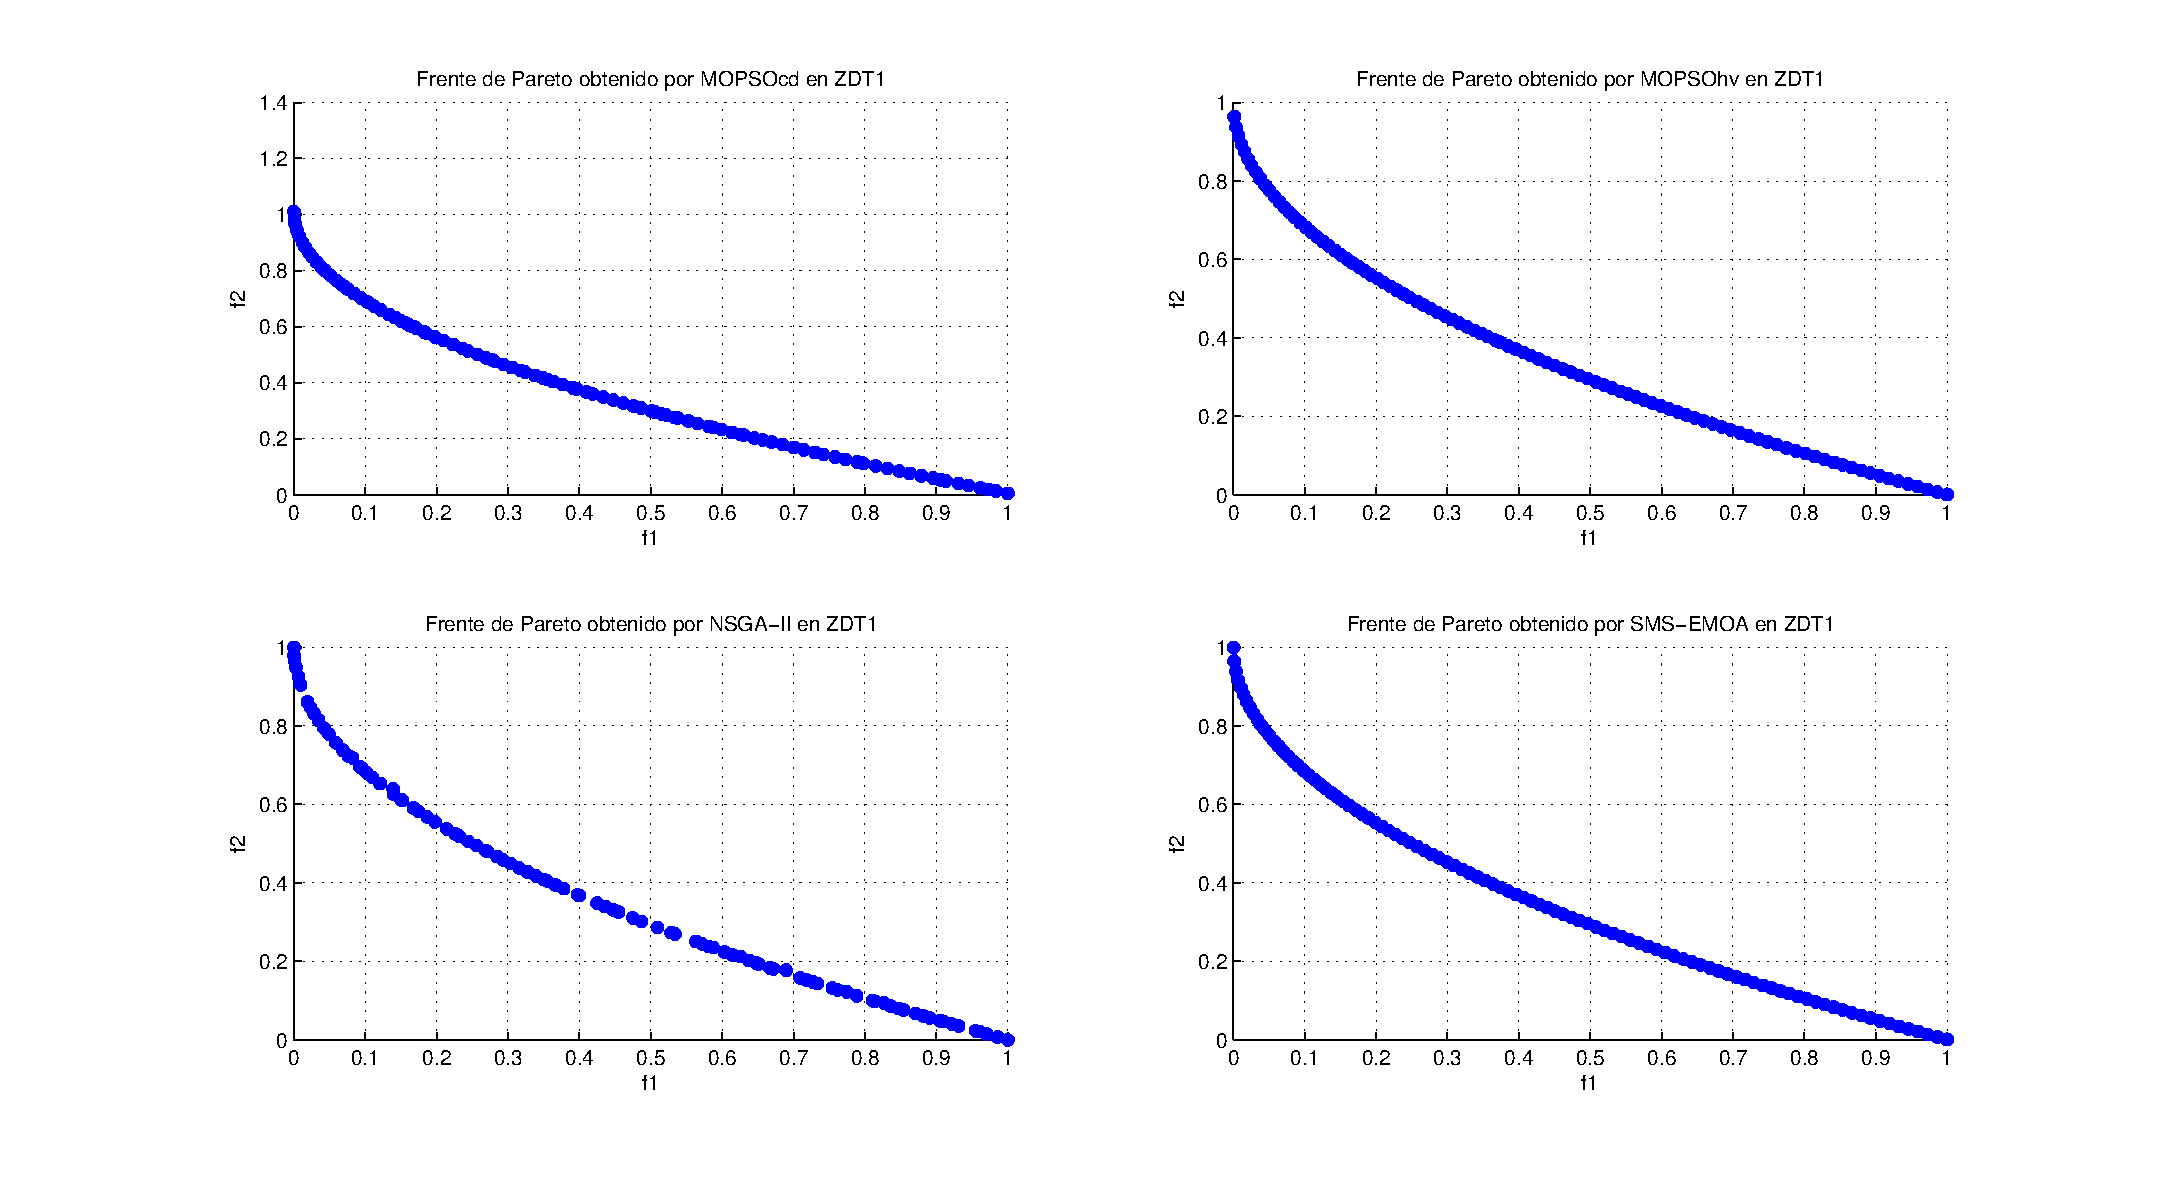
\includegraphics[scale=0.45]{Cap4/rzdt1r.eps}      
%	  \end{rotate}
	\caption{Resultados gr\'aficos correspondientes al problema ZDT1.}
      \label{fig:rZDT1}
      \end{figure}
\clearpage

\newpage
 \begin{table}
 \begin{center}
  \begin{tabular}{|l|cc|cc|} \hline
    & \multicolumn{4}{|c|}{\textbf{Espaciado}} \\ 
	\textbf{Algoritmo} & \textbf{Menor} & \textbf{Mayor} & \textbf{Promedio} & \textbf{Desviaci\'on} \\  \hline\hline
	\textbf{MOPSOhv} &0.004345 & 0.005129 & \textbf{\textcolor{blue}{0.004679}} & \textbf{0.000217}  \\ 
	\textbf{MOPSOcd} &0.006054 & 0.007826 & \textbf{\textcolor{red}{0.007014}} &  \textbf{\textcolor{blue}{0.0005170}}\\ 
	\textbf{NSGA-II} &0.006027 & 0.008074 & \textbf{\textcolor{green}{0.006956}} & \textbf{\textcolor{red}{ 0.000610}}  \\  
	\textbf{SMS-EMOA}&0.002167 & 0.004664 & \textbf{0.004063} & \textbf{\textcolor{green}{0.000543}}  \\  
	\hline\hline
    & \multicolumn{4}{|c|}{\textbf{DGI}} \\ \hline \hline	
	\textbf{MOPSOhv} &0.027389 & 0.027394 & \textbf{\textcolor{green}{0.027391}}& \textbf{\textcolor{green}{0.000001}}  \\ 
	\textbf{MOPSOcd} &0.027462 & 0.027521 & \textbf{\textcolor{red}{0.027497}}  & \textbf{\textcolor{red}{0.000015}}  \\ 
	\textbf{NSGA-II} &0.027386 & 0.027389 & \textbf{\textcolor{blue}{0.027387}} & \textbf{\textcolor{blue}{0.000001}}  \\  
	\textbf{SMS-EMOA}&0.027386 & 0.027387 & \textbf{0.027386} &\textbf{0.000000 } \\  
	\hline\hline
    & \multicolumn{4}{|c|}{\textbf{Hipervolumen}} \\ 	\hline \hline
	\textbf{MOPSOhv} &0.538426 & 0.538666 & \textbf{\textcolor{blue}{0.538568}} & \textbf{\textcolor{blue}{0.000058}} \\ 
	\textbf{MOPSOcd} &0.530732 & 0.534137 & \textbf{\textcolor{red}{0.532098}}  & \textbf{\textcolor{red}{0.000882}}   \\ 
	\textbf{NSGA-II} &0.537163 & 0.537699 & \textbf{\textcolor{green}{0.537424}}& \textbf{\textcolor{green}{0.000148}}  \\  
	\textbf{SMS-EMOA}&0.538808 & 0.538879 & \textbf{0.538872} & \textbf{0.000015}  \\  
	\hline\hline
    & \multicolumn{4}{|c|}{\textbf{Cobertura}} \\ \hline\hline 
	\textbf{Algoritmo} & \textbf{MOPSOhv} & \textbf{MOPSOcd} & \textbf{NSGA-II} & \textbf{SMS-EMOA} \\  \hline \hline
	\textbf{MOPSOhv} &---       &\textbf{0.637500} & \textbf{0.044000}  & \textbf{\textcolor{red}{0.000500}} \\ 
	\textbf{MOPSOcd} & 0.000001 & ---      & 0.003500  & 0.000500 \\ 
	\textbf{NSGA-II} & 0.036500 & 0.589500 & ---      & 0.017500  \\  
	\textbf{SMS-EMOA}& \textbf{0.026500} & 0.665000 & 0.034000 & --- \\  
	\hline
	\end{tabular}
  \caption{Resultados correspondientes al problema ZDT2.}
  \label{tab:zdt2}
\end{center}
\end{table}

La convergencia y la distribuci\'on de las soluciones de nuestra propuesta (MOPSOhv) es buena para este problema, seguido por el SMS-EMOA 
que presenta la mejor convergencia y distribuci\'on (como se muestra en la tabla \ref{tab:zdt2}). Conforme a estos resultados se puede crear una
jerarqu\'ia en orden descendente en t\'erminos de convergencia del conjunto de soluciones pr\'oximas al frente de Pareto real:

\begin{enumerate}
  \item SMS-EMOA
  \item MOPSOhv
  \item NSGA-II
  \item MOPSOcd
\end{enumerate}

Tambi\'en, se observa que en las soluciones de nuestra propuesta dominan a las soluciones del NSGA-II y MOPSOcd, y siendo superado por las 
soluciones del SMS-EMOA.

\clearpage
\newpage
\begin{figure}
      \begin{center}
	  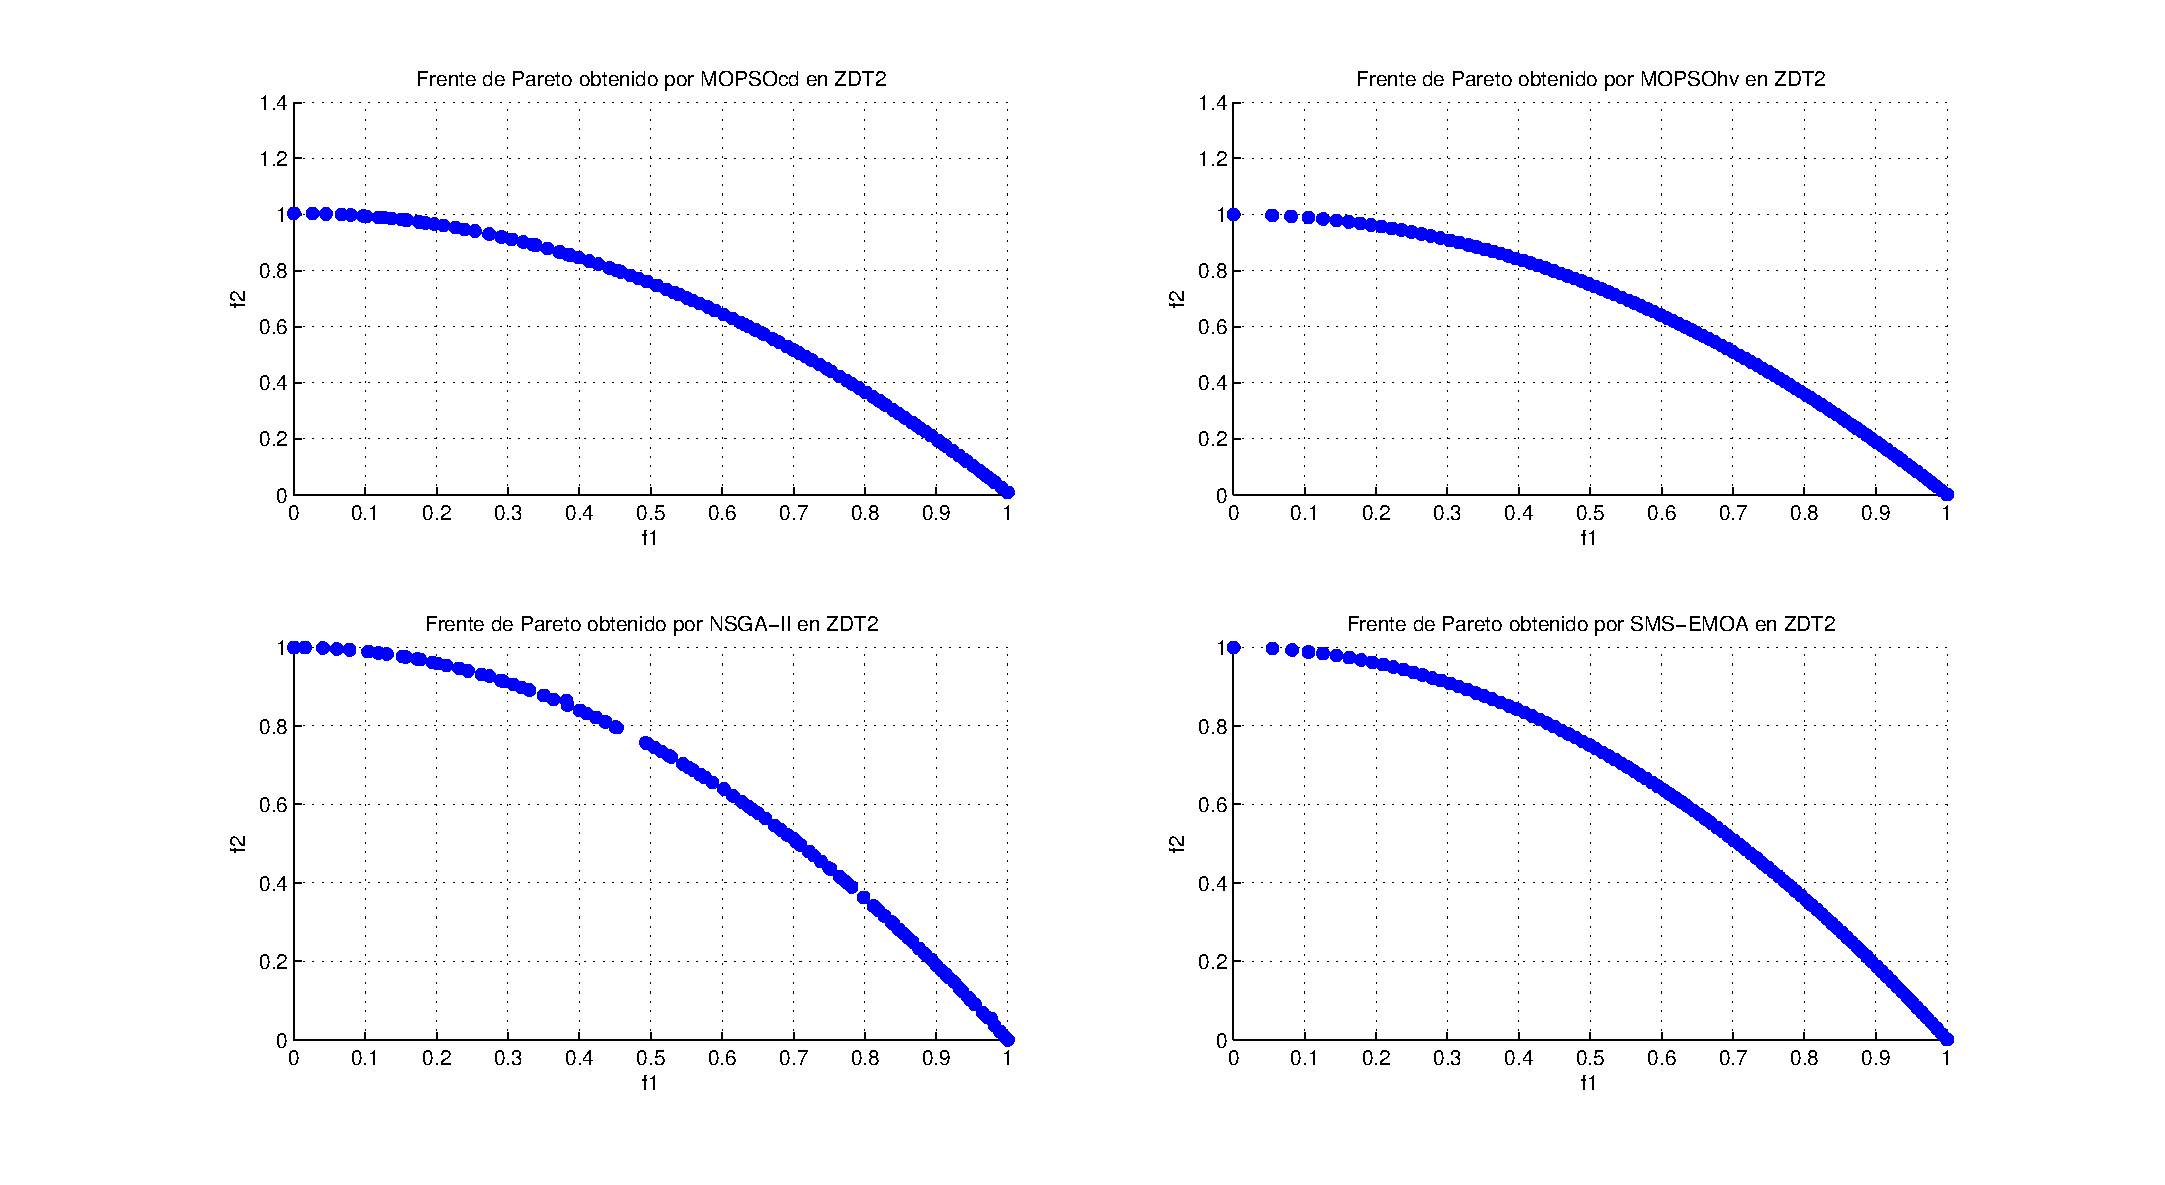
\includegraphics[scale=0.45]{Cap4/rzdt2r.eps}
      \end{center}
	\caption{Resultados gr\'aficos correspondientes al problema ZDT2.}
      \label{fig:rZDT2}
      \end{figure}
\clearpage
\newpage
 \begin{table}
 \begin{center}
  \begin{tabular}{|l|cc|cc|} \hline
    & \multicolumn{4}{|c|}{\textbf{Espaciado}} \\ 
	\textbf{Algoritmo} & \textbf{Menor} & \textbf{Mayor} & \textbf{Promedio} & \textbf{Desviaci\'on} \\  \hline\hline
	\textbf{MOPSOhv} &0.005672 & 0.006958 & \textbf{\textcolor{blue}{0.006248}} & \textbf{\textcolor{blue}{0.000328}}  \\ 
	\textbf{MOPSOcd} &0.007001 & 0.008605 & \textbf{\textcolor{green}{0.007656}}& \textbf{\textcolor{green}{0.000425}} \\ 
	\textbf{NSGA-II} &0.006809 & 0.009101 & \textbf{\textcolor{red}{0.007875}}  & \textbf{\textcolor{red}{0.000565}} \\  
	\textbf{SMS-EMOA}&0.001994 & 0.002563 & \textbf{0.002209} & \textbf{0.000165} \\  
	\hline\hline
    & \multicolumn{4}{|c|}{\textbf{DGI}} \\ 	\hline \hline
	\textbf{MOPSOhv} &0.011174 & 0.011219 & \textbf{\textcolor{blue}{0.011198}} & \textbf{\textcolor{green}{0.000012}} \\ 
	\textbf{MOPSOcd} &0.011389 & 0.011604 & \textbf{\textcolor{green}{0.011492}} & \textbf{\textcolor{red}{0.000064}} \\ 
	\textbf{NSGA-II} &0.011140 & 0.011184 & \textbf{0.011166} & \textbf{\textcolor{blue}{\textbf{0.000016}}} \\  
	\textbf{SMS-EMOA}&0.019892 & 0.019894 & \textbf{\textcolor{red}{0.019892}} & \textbf{0.000001} \\  
	\hline\hline
    & \multicolumn{4}{|c|}{\textbf{Hipervolumen}} \\ \hline \hline
	\textbf{MOPSOhv} &0.952055 & 0.953776 &\textbf{\textcolor{blue}{ 0.952907}} &\textbf{\textcolor{blue}{ 0.000452}}  \\ 
	\textbf{MOPSOcd} &0.936835 & 0.946304 &\textbf{\textcolor{green}{ 0.941991}} &\textbf{\textcolor{green}{ 0.002510}} \\ 
	\textbf{NSGA-II} &0.953544 & 0.954219 & \textbf{0.953912} & \textbf{0.000145}  \\  
	\textbf{SMS-EMOA}&0.522460 & 0.522466 &\textbf{\textcolor{red}{ 0.522464}} & \textbf{\textcolor{red}{0.000001}}  \\  
	\hline
    & \multicolumn{4}{|c|}{\textbf{Cobertura}} \\ \hline\hline 
	\textbf{Algoritmo} & \textbf{MOPSOhv} & \textbf{MOPSOcd} & \textbf{NSGA-II} & \textbf{SMS-EMOA} \\  \hline \hline
	\textbf{MOPSOhv} &---       & \textbf{0.637500} & \textbf{0.044000} & \textbf{\textcolor{red}{0.000500 }}\\ 
	\textbf{MOPSOcd} & 0.000001 & ---      & 0.003500 & 0.000500 \\ 
	\textbf{NSGA-II} & 0.036500 & 0.589500 & ---      & 0.017500 \\  
	\textbf{SMS-EMOA}& \textbf{0.026500} & 0.665000 & 0.034000 & --- \\  
	\hline\hline
	\end{tabular}
\caption{Resultados correspondientes al problema ZDT3.}
  \label{tab:zdt3}
\end{center}
\end{table}

La convergencia y la distribuci\'on de las soluciones de nuestra propuesta (MOPSOhv) es buena para este problema, seguido por el NSGA-II 
que presenta la mejor convergencia y el SMS-EMOA presenta la mejor distribuci\'on (como se muestra en la tabla \ref{tab:zdt3}). Conforme a 
estos resultados se puede crear una jerarqu\'ia en orden descendente en t\'erminos de convergencia del conjunto de soluciones pr\'oximas al 
frente de Pareto real:

\begin{enumerate}
  \item NSGA-II
  \item MOPSOhv
  \item MOPSOcd
  \item SMS-EMOA
\end{enumerate}

Tambi\'en, se observa que en las soluciones de nuestra propuesta dominan a las soluciones del NSGA-II y MOPSOcd, y siendo superado por las 
soluciones del SMS-EMOA.

\clearpage
\newpage
\begin{figure}
      \begin{center}
	  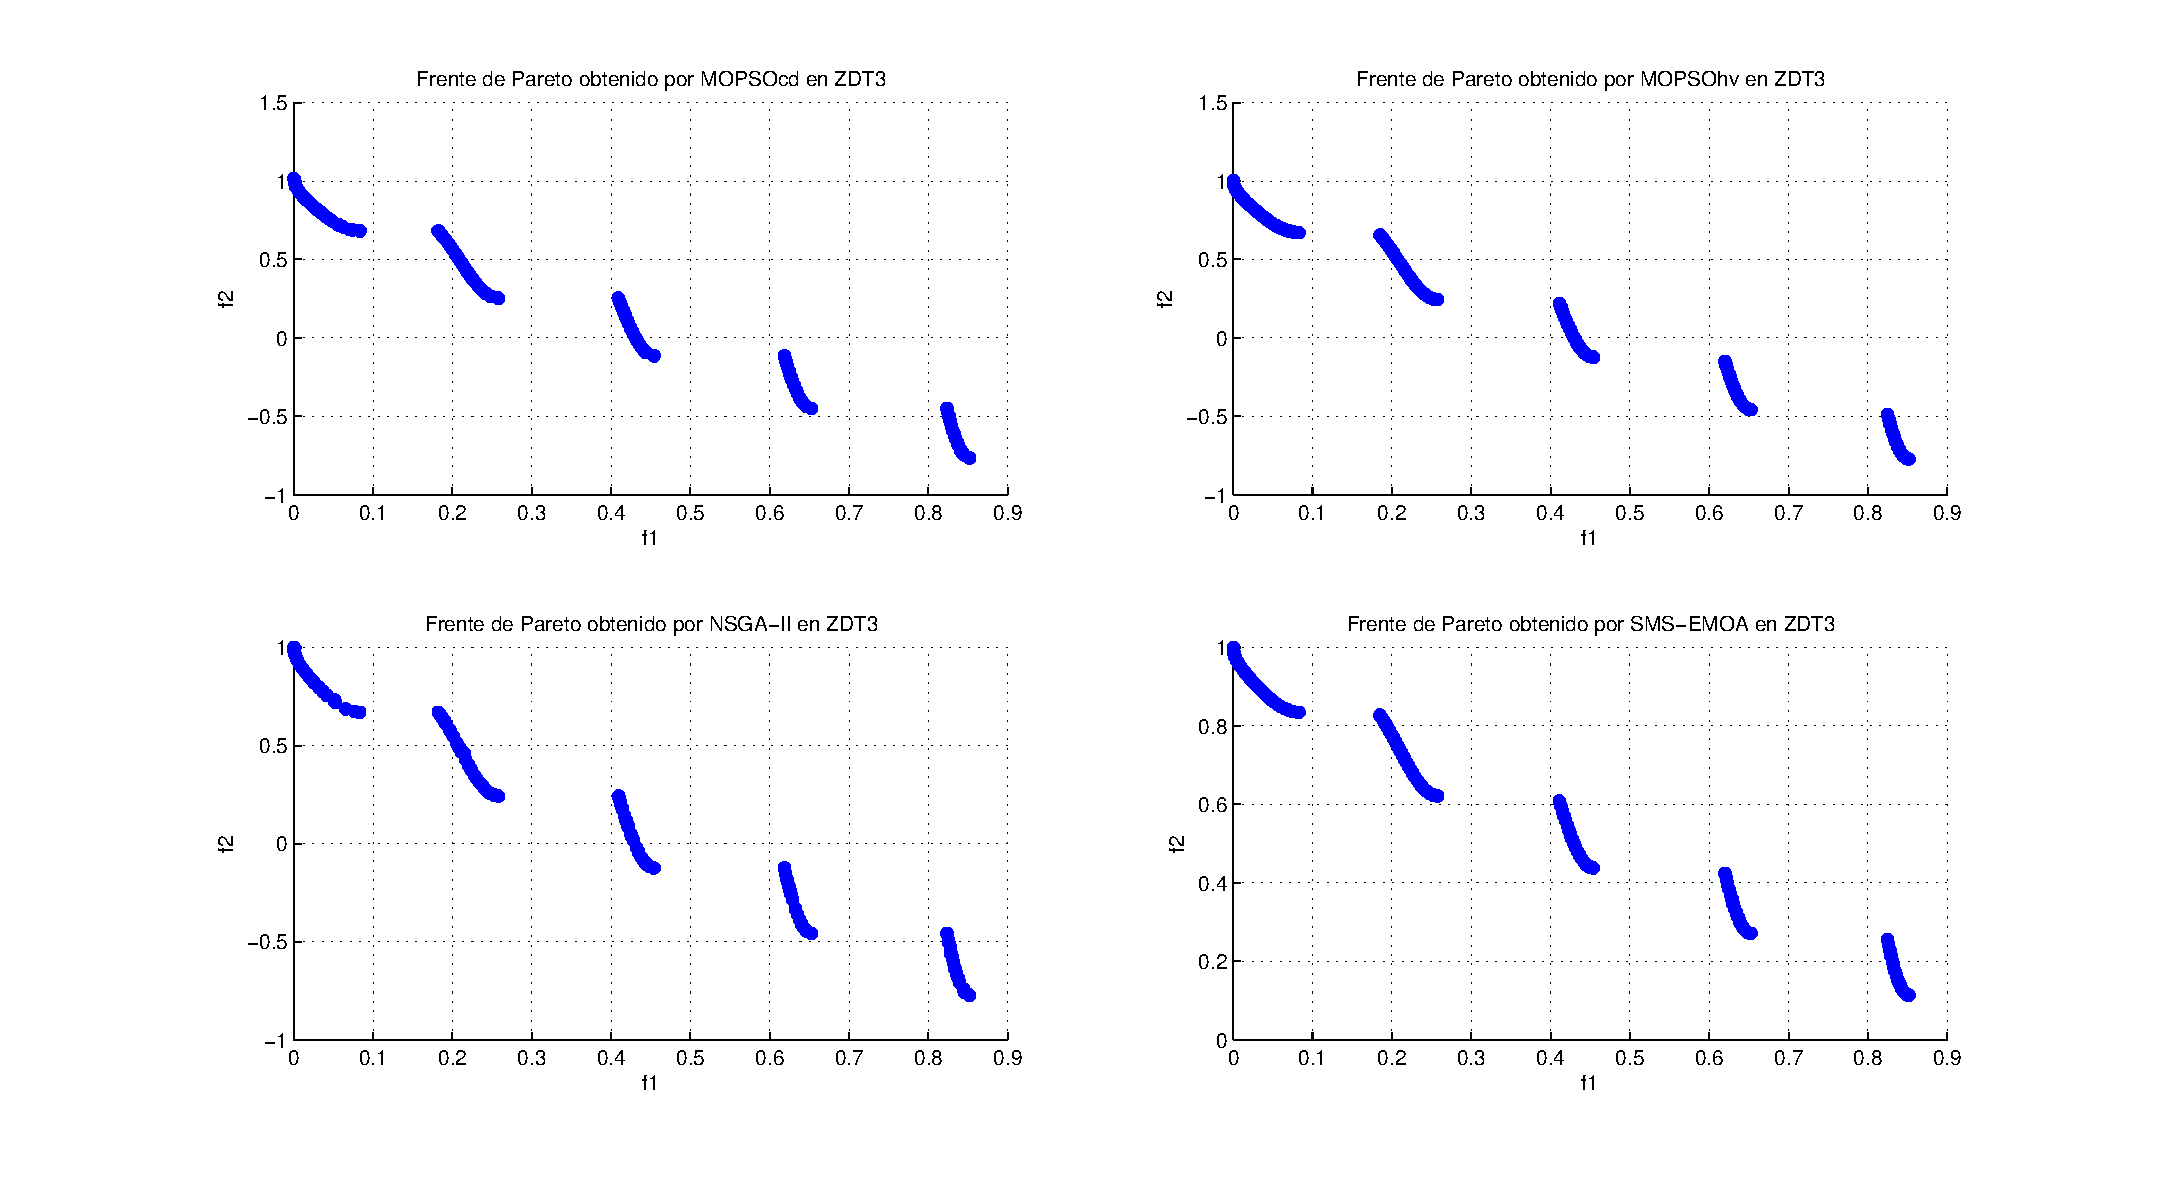
\includegraphics[scale=0.45]{Cap4/rzdt3r.eps}
      \end{center}
	\caption{Resultados gr\'aficos correspondientes al problema ZDT3.}
      \label{fig:rZDT3}
      \end{figure}
\clearpage
\newpage
 \begin{table}
 \begin{center}
  \begin{tabular}{|l|cc|cc|} \hline
    & \multicolumn{4}{|c|}{\textbf{Espaciado}} \\ 
	\textbf{Algoritmo} & \textbf{Menor} & \textbf{Mayor} & \textbf{Promedio} & \textbf{Desviaci\'on} \\  \hline\hline
	\textbf{MOPSOhv} &0.004345 & 0.005129 &\textbf{\textcolor{blue}{ 0.004679}}  &\textbf{ 0.000217} \\ 
	\textbf{MOPSOcd} &0.006054 & 0.007826 &\textbf{\textcolor{green}{ 0.007014}} &\textbf{\textcolor{green}{ 0.000517}}  \\ 
	\textbf{NSGA-II} &0.007089 & 0.009201 &\textbf{\textcolor{red}{ 0.008052}}   &\textbf{\textcolor{red}{ 0.000616}}  \\  
	\textbf{SMS-EMOA}&0.002105 & 0.002981 & \textbf{0.002492} &\textbf{\textcolor{blue}{ 0.000240}}\\  
	\hline\hline
    & \multicolumn{4}{|c|}{\textbf{DGI}} \\ 	\hline \hline
	\textbf{MOPSOhv} &0.027389 & 0.027394 & \textbf{\textcolor{green}{0.027391}} &\textbf{0.000001}   \\ 
	\textbf{MOPSOcd} &0.027462 & 0.027521 & \textbf{\textcolor{red}{0.027497}} & \textbf{\textcolor{red}{0.000015}}  \\ 
	\textbf{NSGA-II} &0.017008 & 0.017016 & \textbf{0.017011} & \textbf{\textcolor{blue}{0.000002}}   \\  
	\textbf{SMS-EMOA}&0.017008 & 0.017030 & \textbf{\textcolor{blue}{0.017011}} & \textbf{\textcolor{green}{0.000004}}  \\  
	\hline\hline
    & \multicolumn{4}{|c|}{\textbf{Hipervolumen}} \\ 	\hline \hline
	\textbf{MOPSOhv} &0.328865 & 0.329046 & \textbf{\textcolor{green}{0.328971}} & \textbf{0.000052}  \\ 
	\textbf{MOPSOcd} &0.323038 & 0.325624 & \textbf{\textcolor{red}{0.324090}} & \textbf{\textcolor{red}{0.000668}}  \\ 
	\textbf{NSGA-II} &0.653158 & 0.654108 & \textbf{\textcolor{blue}{0.653614}} & \textbf{\textcolor{green}{0.000237}}  \\  
	\textbf{SMS-EMOA}&0.654266 & 0.655054 & \textbf{0.654940} & \textbf{\textcolor{blue}{0.000165}}  \\  
	\hline
    & \multicolumn{4}{|c|}{\textbf{Cobertura}} \\ \hline\hline 
	\textbf{Algoritmo} & \textbf{MOPSOhv} & \textbf{MOPSOcd} & \textbf{NSGA-II} & \textbf{SMS-EMOA} \\  \hline \hline
	\textbf{MOPSOhv} & ---      & \textbf{1.000000} & \textbf{0.022500} & \textbf{0.033000} \\ 
	\textbf{MOPSOcd} & 0.000500 & ---      & 0.000001 & 0.000001   \\ 
	\textbf{NSGA-II} & 0.004000 & 1.000000 & ---      & 0.024500 \\  
	\textbf{SMS-EMOA}& 0.000001 & 0.991000 & 0.001000 & --- \\  
	\hline\hline
	\end{tabular}
\caption{Resultados del problema ZDT4.}
  \label{tab:zdt4}
\end{center}
\end{table}

La multimodalidad de ZDT4 causa dificultad a nuestra propuesta (MOPSOhv) para converger de manera \'optima, como se muestra en la 
tabla \ref{tab:zdt4}. Sin embargo, presenta una buena distribuci\'on de las soluciones quedando despu\'es del SMS-EMOA. Nuestra propuesta 
es superada por el SMS-EMOA y NSGA-II y conforme a estos resultados se puede crear una
jerarqu\'ia en orden descendente en t\'erminos de convergencia del conjunto de soluciones pr\'oximas al frente de Pareto real:

\begin{enumerate}
  \item NSGA-II
  \item SMS-EMOA
  \item MOPSOhv
  \item MOPSOcd
\end{enumerate}

Tambi\'en, se observa que en las soluciones de nuestra propuesta dominan a las soluciones de los otros algoritmos.

 \clearpage
 \newpage
 \begin{figure}
      \begin{center}
	  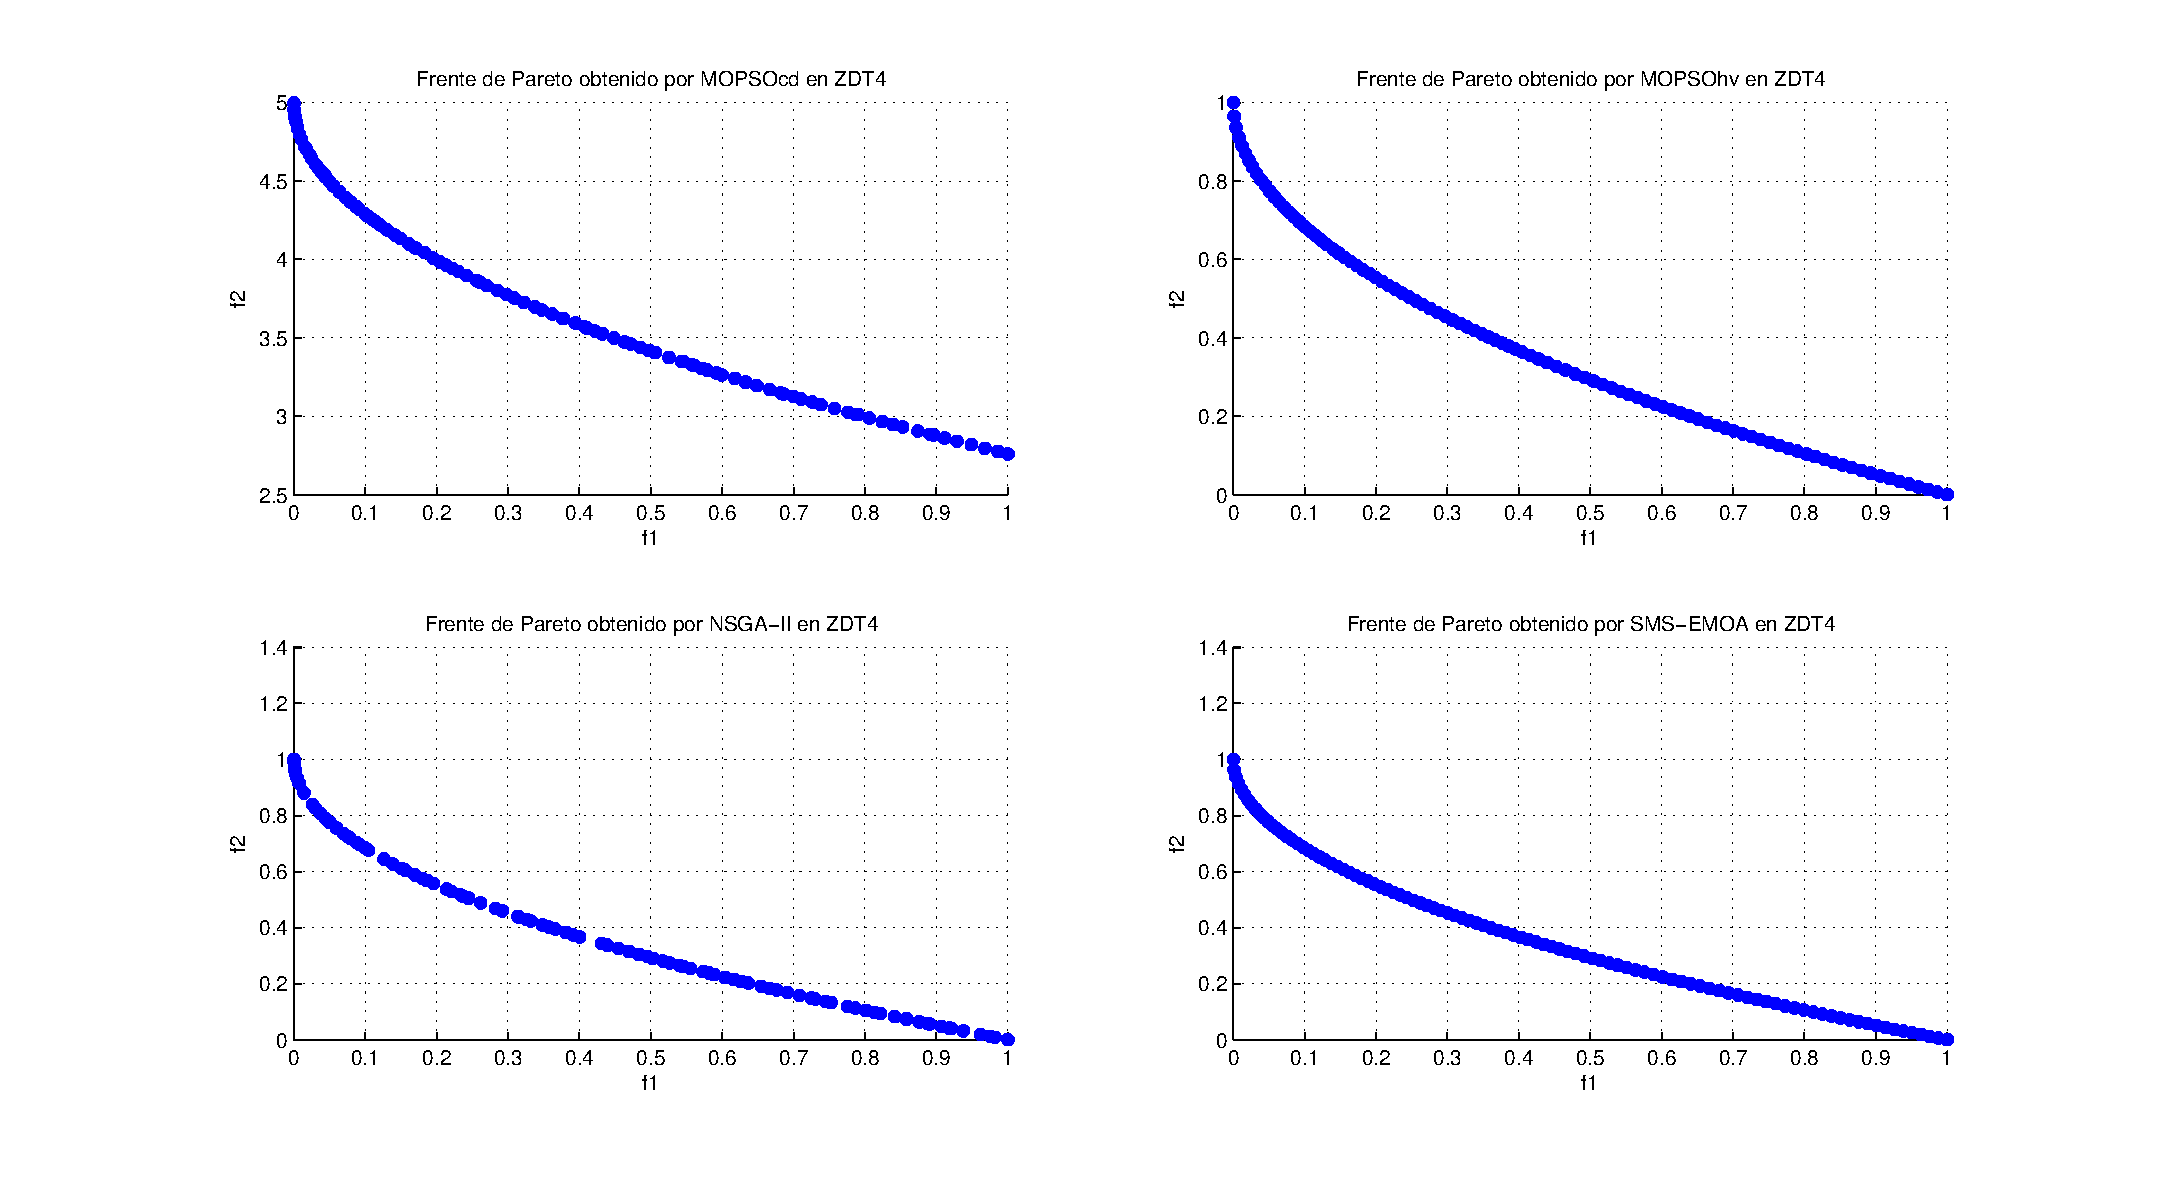
\includegraphics[scale=0.45]{Cap4/rzdt4r.eps}
      \end{center}
	\caption{Resultados gr\'aficos correspondientes al problema ZDT4.}
      \label{fig:rZDT4}
      \end{figure}
 \clearpage
 \newpage
 \begin{table}
 \begin{center}
  \begin{tabular}{|l|cc|cc|} \hline
    & \multicolumn{4}{|c|}{\textbf{Espaciado}} \\ 
	\textbf{Algoritmo} & \textbf{Menor} & \textbf{Mayor} & \textbf{Promedio} & \textbf{Desviaci\'on} \\  \hline\hline
	\textbf{MOPSOhv} &0.001587 & 0.002728 & \textbf{\textcolor{blue}{ 0.001975}} & \textbf{\textcolor{blue}{0.000324}}  \\ 
	\textbf{MOPSOcd} &0.042774 & 0.294482 & \textbf{\textcolor{red}{0.115691}} & \textbf{\textcolor{red}{0.053160}} \\ 
	\textbf{NSGA-II} &0.005925 & 0.007914 & \textbf{\textcolor{green}{0.007055}} & \textbf{\textcolor{green}{0.000437 }} \\  
	\textbf{SMS-EMOA}&0.000256 & 0.001011 & \textbf{0.000603} & \textbf{0.000181} \\  
	\hline\hline
    & \multicolumn{4}{|c|}{\textbf{DGI}} \\ 	\hline \hline
	\textbf{MOPSOhv} &0.027380 & 0.027549 & \textbf{\textcolor{green}{0.027434}} & \textbf{\textcolor{green}{0.000046}}  \\ 
	\textbf{MOPSOcd} &0.000281 & 0.000281 & \textbf{0.000281} & \textbf{0.000000}  \\ 
	\textbf{NSGA-II} &0.017011 & 0.027398 & \textbf{\textcolor{red}{0.026356}} & \textbf{\textcolor{red}{0.003115}}  \\  
	\textbf{SMS-EMOA}&0.027390 & 0.027397 & \textbf{\textcolor{blue}{0.027395}} & \textbf{\textcolor{blue}{0.000002}}  \\  
	\hline\hline
    & \multicolumn{4}{|c|}{\textbf{Hipervolumen}} \\ \hline \hline
	\textbf{MOPSOhv} &0.496939 & 0.54493 & \textbf{\textcolor{blue}{0.512122}} & \textbf{\textcolor{blue}{0.002083}}  \\ 
	\textbf{MOPSOcd} &0.156527 & 0.479775 & \textbf{\textcolor{red}{0.383107}} & \textbf{\textcolor{green}{0.076527}} \\ 
	\textbf{NSGA-II} &0.480422 & 0.870700 & \textbf{0.519667} & \textbf{\textcolor{red}{0.117011}} \\  
	\textbf{SMS-EMOA}&0.503836 & 0.504173 & \textbf{\textcolor{green}{0.503956}} & \textbf{0.000093} \\  
	\hline\hline
    & \multicolumn{4}{|c|}{\textbf{Cobertura}} \\ \hline\hline 
	\textbf{Algoritmo} & \textbf{MOPSOhv} & \textbf{MOPSOcd} & \textbf{NSGA-II} & \textbf{SMS-EMOA} \\  \hline \hline
	\textbf{MOPSOhv} &---       & \textbf{0.127778} & \textbf{\textcolor{red}{0.000001}}  & \textbf{\textcolor{red}{0.000001}} \\ 
	\textbf{MOPSOcd} & 0.059000 & ---      & 0.025500  & 0.019000  \\ 
	\textbf{NSGA-II} & \textbf{0.037500} & 0.645500 & ---       & 0.011000 \\  
	\textbf{SMS-EMOA}& \textbf{0.138889} & 0.850000 & 0.009000  & --- \\  
	\hline
	\end{tabular}
\caption{Resultados correspondientes al problema ZDT6.}
  \label{tab:zdt6}
\end{center}
\end{table}

El espacio de los objetivos para ZDT6 muestra una densidad no uniforme causa dificultad a nuestra propuesta (MOPSOhv) para converger de manera \'optima, 
como se muestra en la tabla \ref{tab:zdt6}. Sin embargo, presenta una buena distribuci\'on de las soluciones quedando despu\'es del SMS-EMOA y 
superando al MOPSOcd, ya que este no es capaz de alcanzar una buena aproximaci\'on al frente de Pareto real. Nuestra propuesta es superada 
por el SMS-EMOA y NSGA-II y conforme a estos resultados se puede crear una
jerarqu\'ia en orden descendente en t\'erminos de convergencia del conjunto de soluciones pr\'oximas al frente de Pareto real:

\begin{enumerate}
  \item NSGA-II
  \item SMS-EMOA
  \item MOPSOhv
  \item MOPSOcd
\end{enumerate}

Tambi\'en, se observa que en las soluciones de nuestra propuesta dominan a las soluciones del MOPSOcd y siendo superado por las soluciones
de manera ligera por el NSGA-II y SMS-EMOA.

\clearpage
\newpage
%\begin{landscape}

  \begin{figure}
      \begin{center}
	  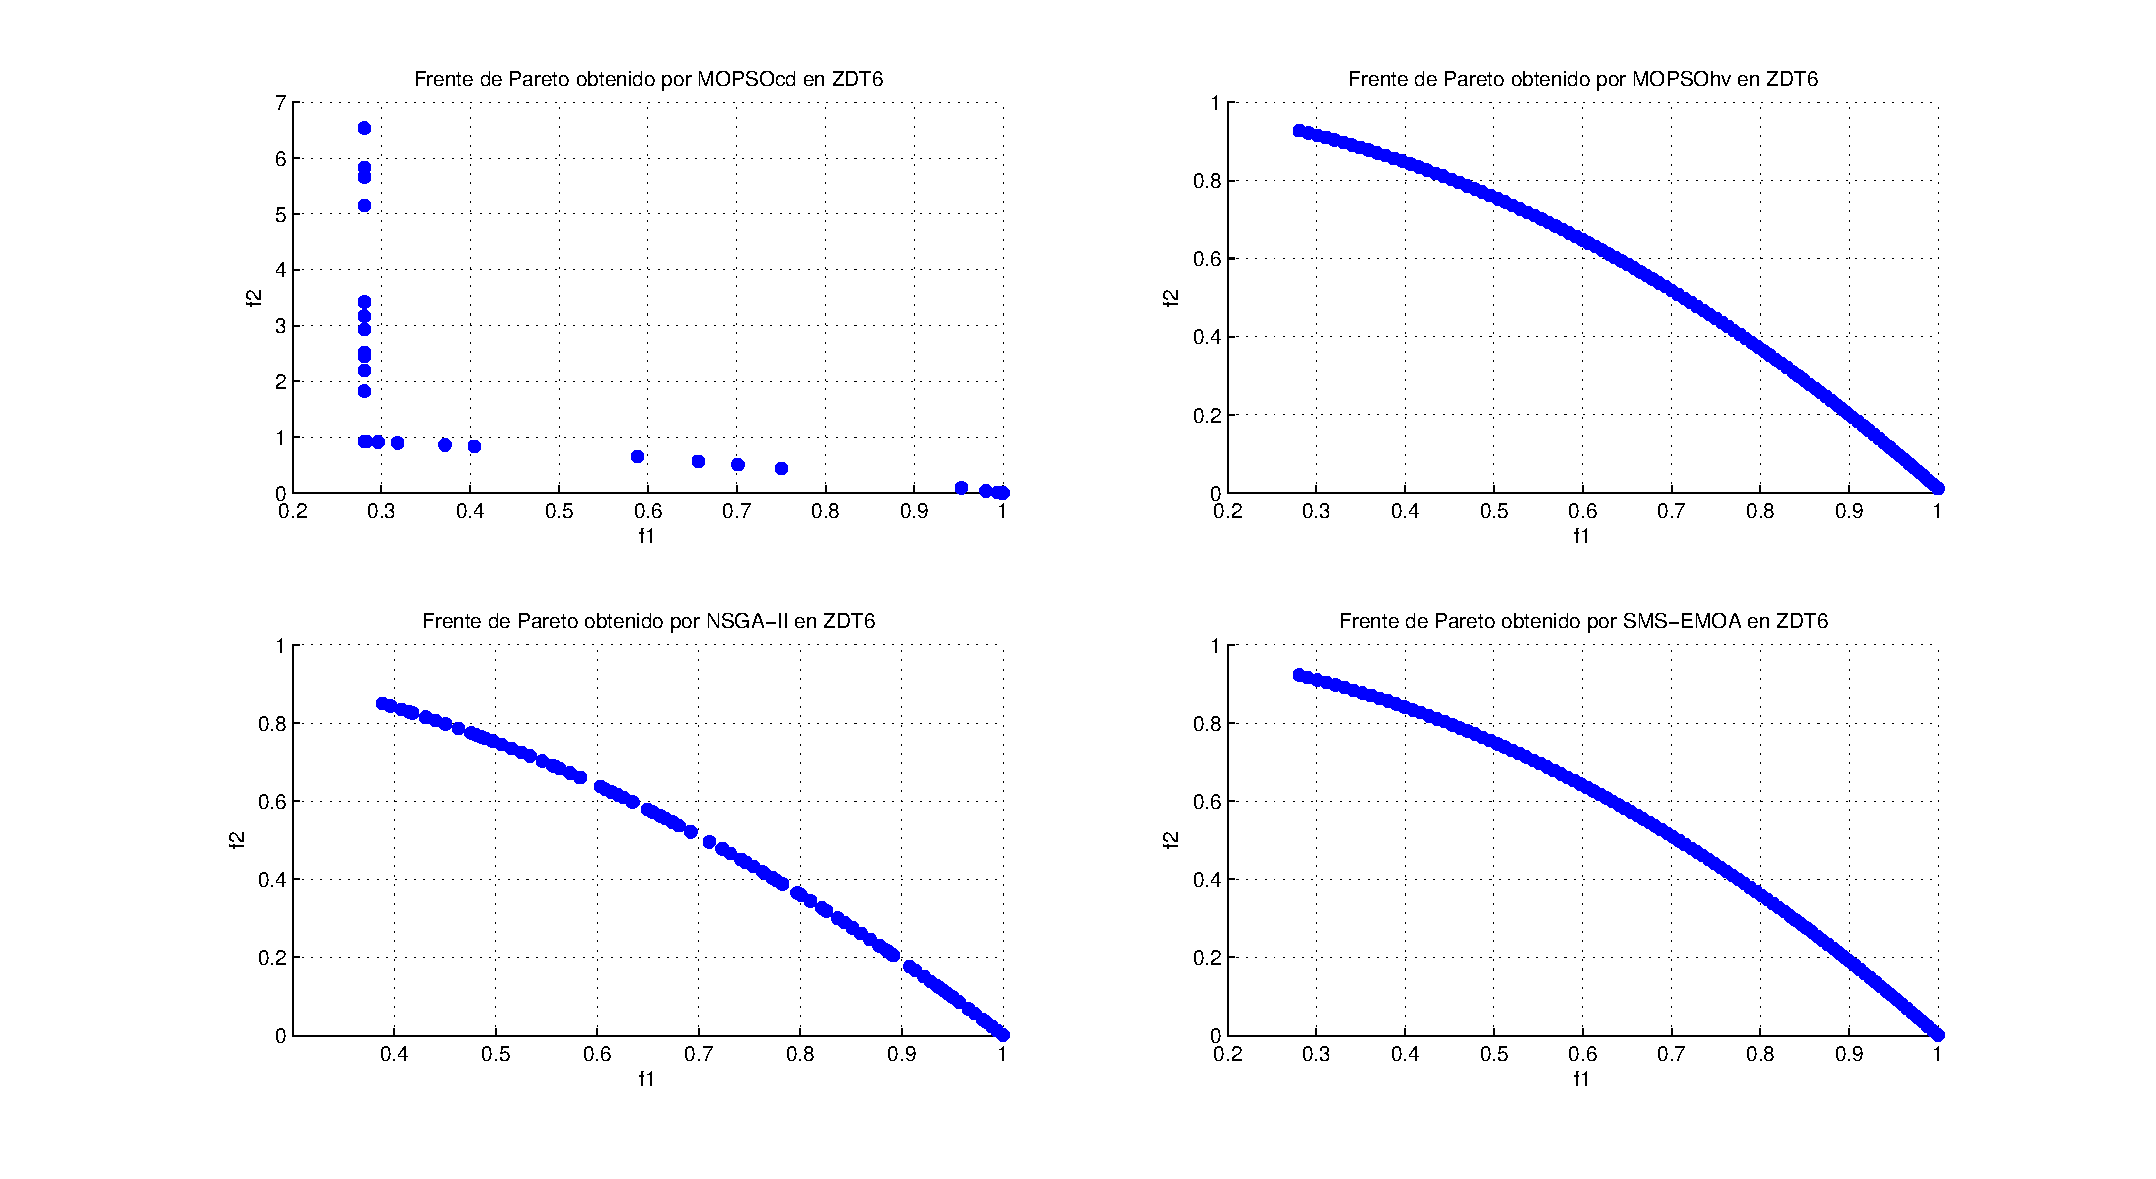
\includegraphics[scale=0.45]{Cap4/rzdt6r.eps}
      \end{center}
	\caption{Resultados gr\'aficos correspondientes al problema ZDT6.}
      \label{fig:rZDT6}
      \end{figure}
%\end{landscape}
\clearpage
   
  
\section{Conjunto de problemas DTLZ} 

Los problemas siguientes son parte de la serie de problemas DTLZ con tres funciones objetivo, tal y como se describen a continuaci\'on 
\cite{dtlz2002a}:

\begin{itemize}
\item La funci\'on de prueba \textbf{DTLZ1} tiene un frente de Pareto lineal, separable y multimodal:

\begin{align*}
f_1(x)&=\frac{1}{2}\cdot x_1\cdot x_2 \cdot \ldots \cdot x_{M-1} \cdot (1+g(x))\\
f_2(x)&=\frac{1}{2}\cdot x_1\cdot x_2 \cdot \ldots \cdot(1-x_{M-1})\cdot(1+g(x))\\
\vdots&\\
f_M(x)&=\frac{1}{2}\cdot(1-x_1)\cdot(1+g(x))\\
g(x)&=100\cdot[k+\sum_{i=M}^n(x_i-0.5)^2-cos(20\cdot\pi\cdot(x_i-0.5))]
\end{align*}

donde $n=M+k-1$ (se sugiere una $k=5$) y $x_i\in[0,1]$ con $i = 1, \ldots, n$ (figura \ref{fig:dtlz1}).


 \item La funci\'on de prueba \textbf{DTLZ2} tiene un frente de Pareto c\'oncavo:
\begin{align*}
f_1(x)&=\cos(x_1\frac{\pi}{2})\cdot\cos(x_2\frac{\pi}{2})\cdot\ldots\cdot\cos(x_{M-1}\frac{\pi}{2})\cdot(1+g(x))\\
f_2(x)&=\cos(x_1\frac{\pi}{2})\cdot\cos(x_2\frac{\pi}{2})\cdot\ldots\cdot\sin(x_{M-1}\frac{\pi}{2})\cdot(1+g(x))\\
f_3(x)&=\cos(x_1\frac{\pi}{2})\cdot\cos(x_2\frac{\pi}{2})\cdot\ldots\cdot\sin(x_{M-2}\frac{\pi}{2})\cdot(1+g(x))\\
\vdots&\\
f_{M-1}(x)&=\cos(x_1\frac{\pi}{2})\cdot\sin(x_2\frac{\pi}{2})(1+g(x))\\
f_{M}(x)&=\sin(x_1\frac{\pi}{2})\cdot(1+g(x))\\
g(x)&=\sum_i=(x_i-0.5)^2
\end{align*}

donde $n=M+k-1$ (se sugiere una $k=10$) y $x_i\in[0,1]$ con $i= 1, \ldots, n$. Este problema se puede utilizar para investigar la 
escalabilidad (figura \ref{fig:dtlz2}).

\item La funci\'on de prueba \textbf{DTLZ3} tiene un frente de Pareto c\'oncavo y multimodal:
\begin{align*}
f_1(x)&=\cos(x_1\frac{\pi}{2})\cdot\cos(x_2\frac{\pi}{2})\cdot\ldots\cdot \cos(x_{M-1}\frac{\pi}{2})\cdot(1+g(x))\\
f_2(x)&=\cos(x_1\frac{\pi}{2})\cdot\cos(x_2\frac{\pi}{2})\cdot\ldots\cdot \sin(x_{M-1}\frac{\pi}{2})\cdot(1+g(x))\\
f_3(x)&=\cos(x_1\frac{\pi}{2})\cdot\cos(x_2\frac{\pi}{2})\cdot\ldots\cdot \sin(x_{M-2}\frac{\pi}{2})\cdot(1+g(x))\\
\vdots&\\
f_{M-1}(x)&=\cos(x_1\frac{\pi}{2})\cdot\sin(x_2\frac{\pi}{2})\cdot(1+g(x))\\
f_{M}(x)&=\sin(x_1\frac{\pi}{2})\cdot (1+g(x))\\
g(x)&=100\cdot [k+\sum_{i=M}^n(x_i-0.5)^2-\cos(20\cdot\pi\cdot(x_i-0.5))]
\end{align*}

donde $n=M+k-1$ (se sugiere una $k=10$) y $x_i\in[0,1]$ con $i=1, \ldots, n$. La forma del frente de Pareto de este
problema es similar al del problema DTLZ2 (figura \ref{fig:dtlz2}).

\item La funci\'on de prueba \textbf{DTLZ4} tiene un frente de Pareto c\'oncavo, separable y multimodal:

\begin{align*}
f_1(x)&=\cos(x_1^\alpha\frac{\pi}{2})\cdot\cos(x_2^\alpha\frac{\pi}{2})\cdot\ldots\cdot \cos(x_{M-1}^\alpha\frac{\pi}{2})\cdot(1+g(x))\\
f_2(x)&=\cos(x_1^\alpha\frac{\pi}{2})\cdot\cos(x_2^\alpha\frac{\pi}{2})\cdot\ldots\cdot \sin(x_{M-1}^\alpha\frac{\pi}{2})\cdot(1+g(x))\\
f_3(x)&=\cos(x_1^\alpha\frac{\pi}{2})\cdot\cos(x_2^\alpha\frac{\pi}{2})\cdot\ldots\cdot \sin(x_{M-2}^\alpha\frac{\pi}{2})\cdot(1+g(x))\\
\vdots&\\
f_{M-1}(x)&=\cos(x_1^\alpha\frac{\pi}{2})\cdot\sin(x_2^\alpha\frac{\pi}{2})\cdot(1+g(x))\\
f_{M}(x)&=\sin(x_1^\alpha\frac{\pi}{2})\cdot(1+g(x))\\
g(x)&=\sum_i(x_i-0.5)^2
\end{align*}

donde $n=M+k-1$ (se sugiere una $k=10$ y $\alpha=100$) y $x_i\in[0,1]$ con $i=1,\ldots, n$. Este problema prueba la habilidad de mantener 
una buena distribuci\'on de las soluciones. La forma del frente de Pareto de este
problema es similar al del problema DTLZ2 (figura \ref{fig:dtlz2}).

\item \textbf La funci\'on de prueba \textbf{DTLZ5} tiene un frente de Pareto curvo:

\begin{align*}
f_1(x)&=\cos(\theta_1\frac{\pi}{2})\cdot\cos(\theta_2\frac{\pi}{2})\cdot\ldots\cdot \cos(\theta_{M-1}\frac{\pi}{2})\cdot(1+g(x))\\
f_2(x)&=\cos(\theta_1\frac{\pi}{2})\cdot\cos(\theta_2\frac{\pi}{2})\cdot\ldots\cdot \sin(\theta_{M-1}\frac{\pi}{2})\cdot(1+g(x))\\
f_3(x)&=\cos(\theta_1\frac{\pi}{2})\cdot\cos(\theta_2\frac{\pi}{2})\cdot\ldots\cdot \sin(\theta_{M-2}\frac{\pi}{2})\cdot(1+g(x))\\
\vdots&\\
f_{M-1}(x)&=\cos(\theta_1\frac{\pi}{2})\cdot\sin(\theta_2\frac{\pi}{2})\cdot(1+g(x))\\
f_{M}(x)&=\sin(\theta_1\frac{\pi}{2})\cdot(1+g(x))\\
\theta_1&=\frac{\pi}{2}x_1\\
\theta_i&=\frac{\pi}{4\cdot(1+g(x))}(1+2\cdot g(x)\cdot x_i),  \text{para} \hspace{1mm} i=2,3\dots,(M-1)\\
g(x)&=\sum^n_i(x_i-0.5)^2
\end{align*}

donde $n=M+k-1$ (se sugiere una $k=10$) y $x_i\in[0,1]$ con $i = 1,\ldots,n$ (figura \ref{fig:dtlz5}).

\item La funci\'on de prueba \textbf{DTLZ6} tiene un frente de Pareto curvo:

\begin{align*}
f_1(x)&=\cos(\theta_1\frac{\pi}{2})\cdot\cos(\theta_2\frac{\pi}{2})\cdot\ldots\cdot \cos(\theta_{M-1}\frac{\pi}{2})\cdot(1+g(x))\\
f_2(x)&=\cos(\theta_1\frac{\pi}{2})\cdot\cos(\theta_2\frac{\pi}{2})\cdot\ldots\cdot \sin(\theta_{M-1}\frac{\pi}{2})\cdot(1+g(x))\\
f_3(x)&=\cos(\theta_1\frac{\pi}{2})\cdot\cos(\theta_2\frac{\pi}{2})\cdot\ldots\cdot \sin(\theta_{M-2}\frac{\pi}{2})\cdot(1+g(x))\\
\vdots&\\
f_{M-1}(x)&=\cos(\theta_1\frac{\pi}{2})\cdot\sin(\theta_2\frac{\pi}{2})\cdot(1+g(x))\\
f_{M}(x)&=\sin(\theta_1\frac{\pi}{2})\cdot(1+g(x))\\
\theta_1&=\frac{\pi}{2}x_1\\
\theta_i&=\frac{\pi}{4(1+g(x))}(1+2\cdot g(x)\cdot x_i),  \text{para}\hspace{1mm} i=2,3\dots,(M-1)\\
g(x)&=\sum^n_i=(x_i-0.5)^0.1
\end{align*}

donde $n=M+k-1$ (se sugiere una $k=10$) y $x_i\in[0,1]$ con $i=1,\ldots,n$ (figura \ref{fig:dtlz6}).

\item La funci\'on de prueba \textbf{DTLZ7} tiene un frente de Pareto discontinuo:

\begin{align*}
f_1(x)&=x_1 \\
f_2(x)&=x_2\\
\vdots&\\
f_{M-1}(x)&=x_{M-1}\\
f_{M}(x)&=(1+g(x_M))\cdot h(f_1,f_2,\dots,f_{M-1}g(x))\\
g(x)&=1+\frac{9}{k}\cdot\sum_{i=2}^nx_i\\
h(f_1,f_2,\dots,f_{M-1}g(x))&=M-\sum_{i=1}^{M-1}(\frac{f_i}{1+g(x)}(1+\sin{(3\cdot\pi\cdot f_i)}))
\end{align*}

donde $n=M+k-1$ (se sugiere una $k=20$) y $x_i\in[0,1]$ con $i=1,\ldots,n$. Este problema prueba la habilidad de mantener 
individuos en las diferentes regiones del frente de Pareto (figura \ref{fig:dtlz7}).

\end{itemize}


\begin{figure}
    \centering
    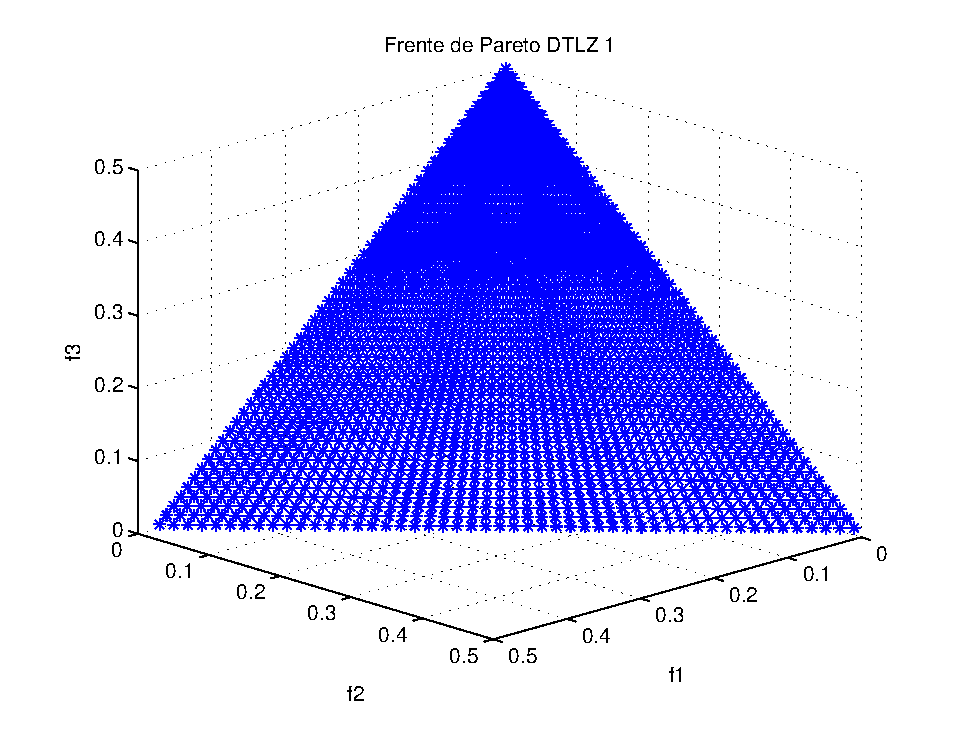
\includegraphics[scale=0.7]{ApendiceA/paretoDTLZ1.eps}
    \caption{Frente de Pareto verdadero de DTLZ1}
    \label{fig:dtlz1}
\end{figure}

\begin{figure}
    \centering
    \includegraphics[scale=0.7]{ApendiceA/paretoDTLZ2.eps}
    \caption{Frente de Pareto verdadero de DTLZ2}
    \label{fig:dtlz2}
\end{figure}
2\begin{figure}
    \centering
    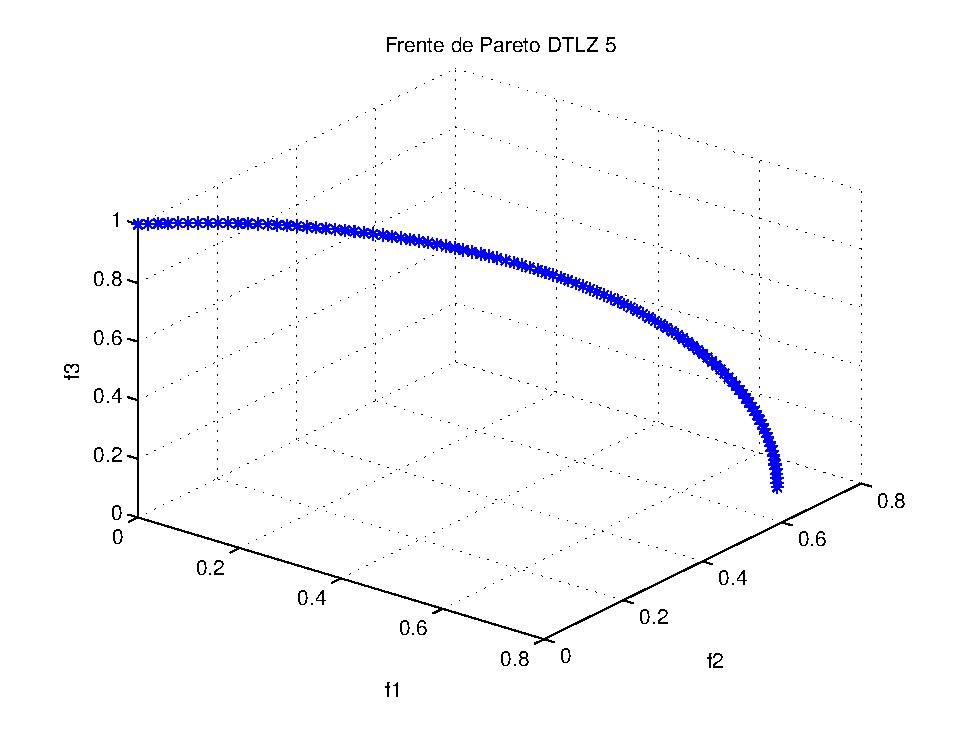
\includegraphics[scale=0.7]{ApendiceA/paretoDTLZ5.eps}
    \caption{Frente de Pareto verdadero de DTLZ5}
    \label{fig:dtlz5}
\end{figure}
\begin{figure}
  \centering
    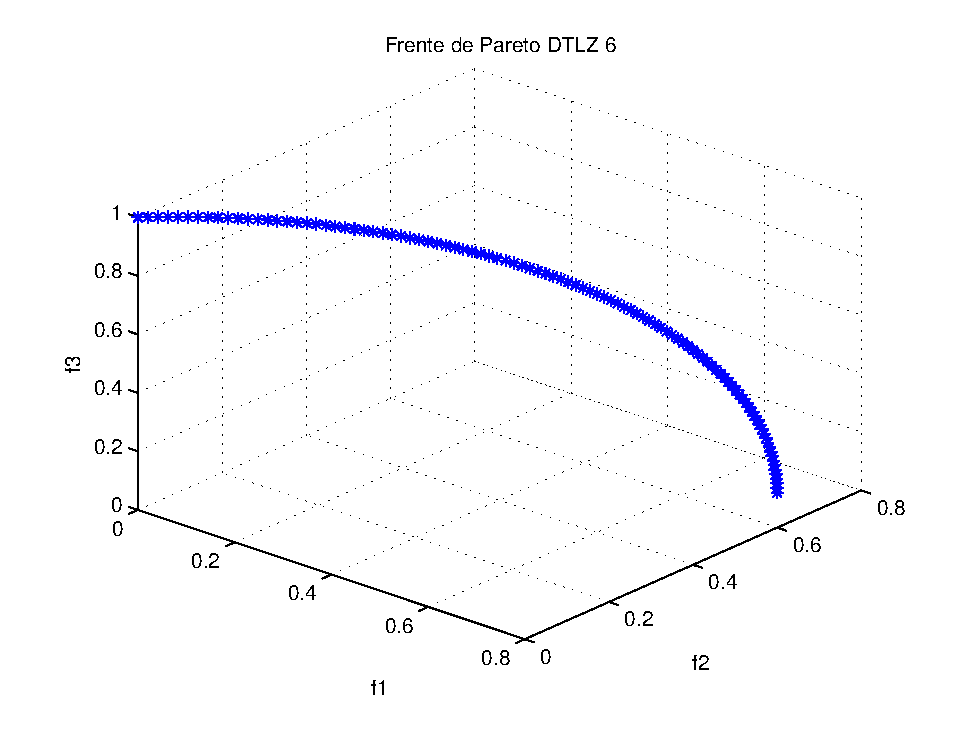
\includegraphics[scale=0.7]{ApendiceA/paretoDTLZ6.eps}
    \caption{Frente de Pareto verdadero de DTLZ6}
   \label{fig:dtlz6}
\end{figure}
\begin{figure}
 \centering
    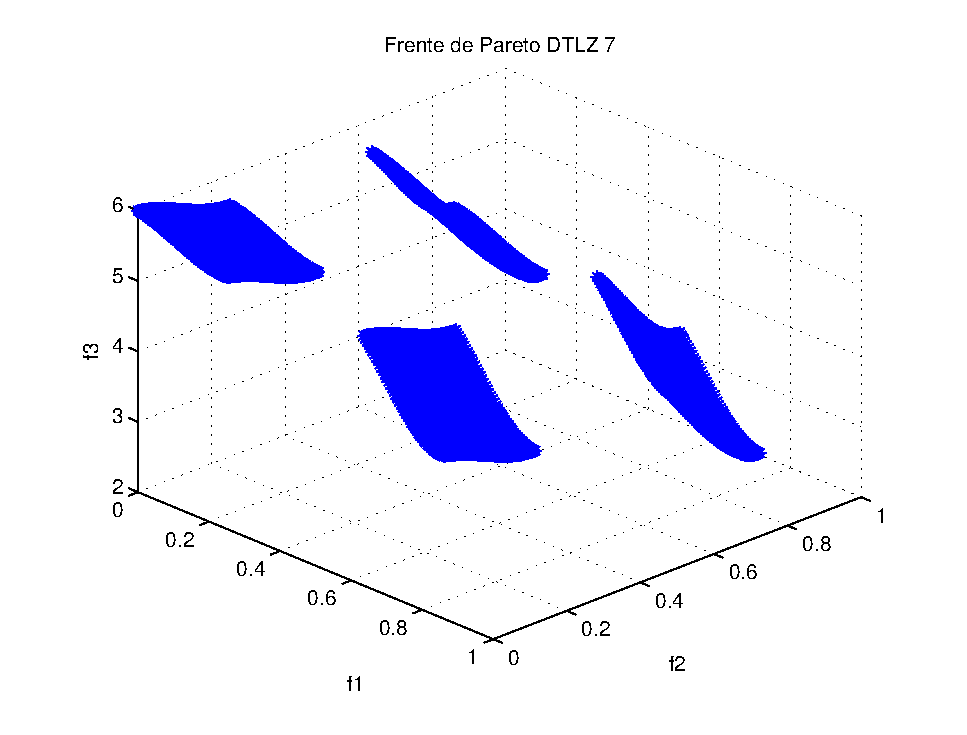
\includegraphics[scale=0.7]{ApendiceA/paretoDTLZ7.eps}
    \caption{Frente de Pareto verdadero de DTLZ7}
    \label{fig:dtlz7}
\end{figure}

\newpage

\section{Evaluaci\'on del conjunto de problemas DTLZ}

Para calcular la m\'etrica del hipervolumen se utiliza como punto de referencia el mostrado en la tabla \ref{tab:refdtlz}.

Los resultados obtenidos por nuestra propuesta (MOPSOhv) para los problemas DTLZ1, DTLZ3 y DTLZ6 son mejores que los obtenidos por el MOPSOcd,
ya que las soluciones de nuestra propuesta, seg\'un la m\'etrcia de cobertura, dominan completamente las soluciones arrojadas por MOPSOcd. 
Sin embargo, los resultados de nuestra propuesta son malos en comparaci\'on con los obtenidos por SMS-EMOA y NSGA-II, los cuales 
obtuvieron soluciones que dominan completamente a las nuestras como se muestra en las tablas \ref{tab:dtlz1}, \ref{tab:dtlz3} y \ref{tab:dtlz6}. 

  Conforme a estos resultados se tiene una jerarqu\'ia en orden descendente en t\'erminos de convergencia en estos primeros tres 
  problemas:

\begin{enumerate}
  \item NSGA-II
  \item SMS-EMOA
  \item MOPSOhv
  \item MOPSOcd
\end{enumerate}

El problema DTLZ4 presenta un frente de Pareto c\'oncavo. En la la figura \ref{fig:rDTLZ4} se muestran como los 
resultados obtenidos por nuestra propuesta (MOPSOhv) se distribuyen hacia los extremos del frente de Pareto, lo que causa tener una menor 
cobertura sobre \'este y causando que el valor en 
la m\'etrica del hipervolumen sea menor que los otros algoritmos. Sin embargo, las soluciones dominan a las soluciones de los 
dem\'as algoritmos como se muestra en la tabla \ref{tab:dtlz4}.

El problema DTLZ5 presenta un frente de Pareto curvo. DTLZ5 se considera un problema f\'acil, ya que su espacio de b\'usqueda 
presenta sesgo hacia soluciones cercanas al frente de Pareto verdadero. La figura \ref{fig:rDTLZ5} muestra que los resultados son similares 
para todos los algoritmos. Sin embargo, nuestras soluciones (MOPSOhv) dominan a las soluciones de los dem\'as algoritmos
excepto por las de SMS-EMOA como se muestra en la tabla \ref{tab:dtlz5}.

El problema DTLZ7 presenta un frente de Pareto con regiones discontinuas. Los resultados de nuestra propuesta (MOPSOhv) son similares que los de 
los algoritmos NSGA-II y MOPSOcd. Sin embargo, nuestras soluciones son dominadas por las obtenidas por SMS-EMOA
(tabla \ref{tab:dtlz7}). La figura \ref{fig:rDTLZ7} muestra como las soluciones se concentran en una parte del frente de Pareto.

 Conforme a estos resultados se tiene una jerarqu\'ia general en orden descendente en t\'erminos de convergencia para  
 DTLZ4, DTLZ5 y DTLZ7 problemas:

\begin{enumerate}
  \item  NSGA-II
  \item SMS-EMOA
  \item MOPSOhv
  \item MOPSOcd
\end{enumerate}

\begin{table}
  \begin{center}
    \begin{tabular}{|l||c|}
	\hline
	Problema  & Punto de referencia \\ 
	\hline
	\hline
	DTLZ1 & $(1.1,1.1,1.1)$ \\ 
	\hline
	DTLZ2 &  $(1.1,1.1,1.1)$\\
	\hline
	DTLZ3 &  $(5.0,5.0,5.0)$\\
	\hline
	DTLZ4 &  $(1.1,1.1,1.1)$\\
	\hline
	DTLZ5 &  $(1.1,1.1,1.1)$\\
	\hline
	DTLZ6 &  $(1.1,1.1,1.1)$\\
	\hline
	DTLZ7 &  $(1.1,1.1,7.0)$\\
	\hline
  \end{tabular}
  \caption{Puntos de referencia utilizados para el conjunto de problemas DTLZ}
  \label{tab:refdtlz}
\end{center}
\end{table}
\clearpage
\newpage
\begin{table}
 \begin{center}
  \begin{tabular}{|l|cc|cc|} \hline
    & \multicolumn{4}{|c|}{Espaciado} \\ 
	\textbf{Algoritmo} & \textbf{Menor} & \textbf{Mayor} & \textbf{Promedio} & \textbf{Desviaci\'on} \\  \hline \hline
	MOPSOhv &0.026239 & 0.184637 &  \textbf{\textcolor{green}{0.081790}} &  \textbf{\textcolor{green}{0.045829}}    \\ 
	MOPSOcd &0.531066 & 1.547502 &  \textbf{\textcolor{red}{0.974734}} &  \textbf{\textcolor{red}{0.295577}}   \\ 
	NSGA-II &0.015203 & 0.023959 &  \textbf{\textcolor{blue}{0.019360}} & \textbf{\textcolor{blue}{ 0.002384  }} \\  
	SMS-EMOA&0.005793 & 0.012914 & \textbf{0.006947} &  \textbf{0.001461}   \\  
	\hline\hline
    & \multicolumn{4}{|c|}{DGI} \\ \hline\hline
	MOPSOhv &0.000617 & 0.035965 &  \textbf{\textcolor{green}{0.013359}} &  \textbf{\textcolor{green}{0.011381}}  \\ 
	MOPSOcd &0.145461 & 0.462595 &  \textbf{\textcolor{red}{0.269641}} &  \textbf{\textcolor{red}{0.080597}}  \\ 
	NSGA-II &0.000540 & 0.003699 & \textbf{0.001261} &  \textbf{\textcolor{red}{0.001148}}   \\  
	SMS-EMOA &0.005777 & 0.011575 &  \textbf{\textcolor{blue}{0.006088}} &  \textbf{\textcolor{blue}{0.001259}}  \\  
	\hline\hline
    & \multicolumn{4}{|c|}{Hipervolumen} \\ 
  \hline\hline
	MOPSOhv &0.000000 & 1.290672 &  \textbf{\textcolor{green}{0.838140}} & \textbf{\textcolor{green}{0.351522}}  \\ 
	MOPSOcd &0.000000 & 0.000000 &  \textbf{\textcolor{red}{0.000000}} &  \textbf{\textcolor{red}{0.000000}}  \\ 
	NSGA-II &1.244198 & 1.297406 &  \textbf{\textcolor{blue}{1.270538}} &  \textbf{0.016839}  \\  
	SMS-EMOA &1.123310 & 1.305100 &\textbf{ 1.295857} &  \textbf{\textcolor{blue}{0.039586}}  \\  
	\hline\hline
	& \multicolumn{4}{|c|}{\textbf{Cobertura}} \\ \hline\hline 
	\textbf{Algoritmo} & \textbf{MOPSOhv} & \textbf{MOPSOcd} & \textbf{NSGA-II} & \textbf{SMS-EMOA} \\  \hline \hline
	\textbf{MOPSOhv} & ---      & \textbf{0.964500} &  \textbf{\textcolor{red}{0.000000}} &  \textbf{\textcolor{red}{0.000000}}  \\ 
	\textbf{MOPSOcd} & 0.000000 & ---      &  0.000000  & 0.000000 \\ 
	\textbf{NSGA-II} & \textbf{0.838500} & 0.977500 & ---       & 0.039000 \\  
	\textbf{SMS-EMOA}& \textbf{0.771000} & 0.911500 & 0.000000  & --- \\  
	\hline
	\end{tabular}
\caption{Resultados correspondientes al problema DTLZ1.}
  \label{tab:dtlz1}
\end{center}
\end{table}
La multimodalidad de DTLZ1 causa dificultad a nuestra propuesta (MOSPSOhv) para converger de manera \'optima, como se muestra en la 
tabla \ref{tab:dtlz1}. En la gr\'afica \ref{fig:rDTLZ1} se muestra que el MOPSOcd no tiene una buena convergencia
al frente de Pareto y no muestra una buena distribuci\'on de las soluciones, por lo que nuestra propuesta se mantienen arriba de \'este.
Sin embargo, nuestra propuesta es superada por el SMS-EMOA y NSGA-II y conforme a estos resultados se puede crear una
jerarqu\'ia en orden descendente en t\'erminos de convergencia del conjunto de soluciones pr\'oximas al frente de Pareto real:

\begin{enumerate}
  \item NSGA-II
  \item SMS-EMOA
  \item MOPSOhv
  \item MOPSOcd
\end{enumerate}

\clearpage
\newpage

\begin{figure}
      \begin{center}
	  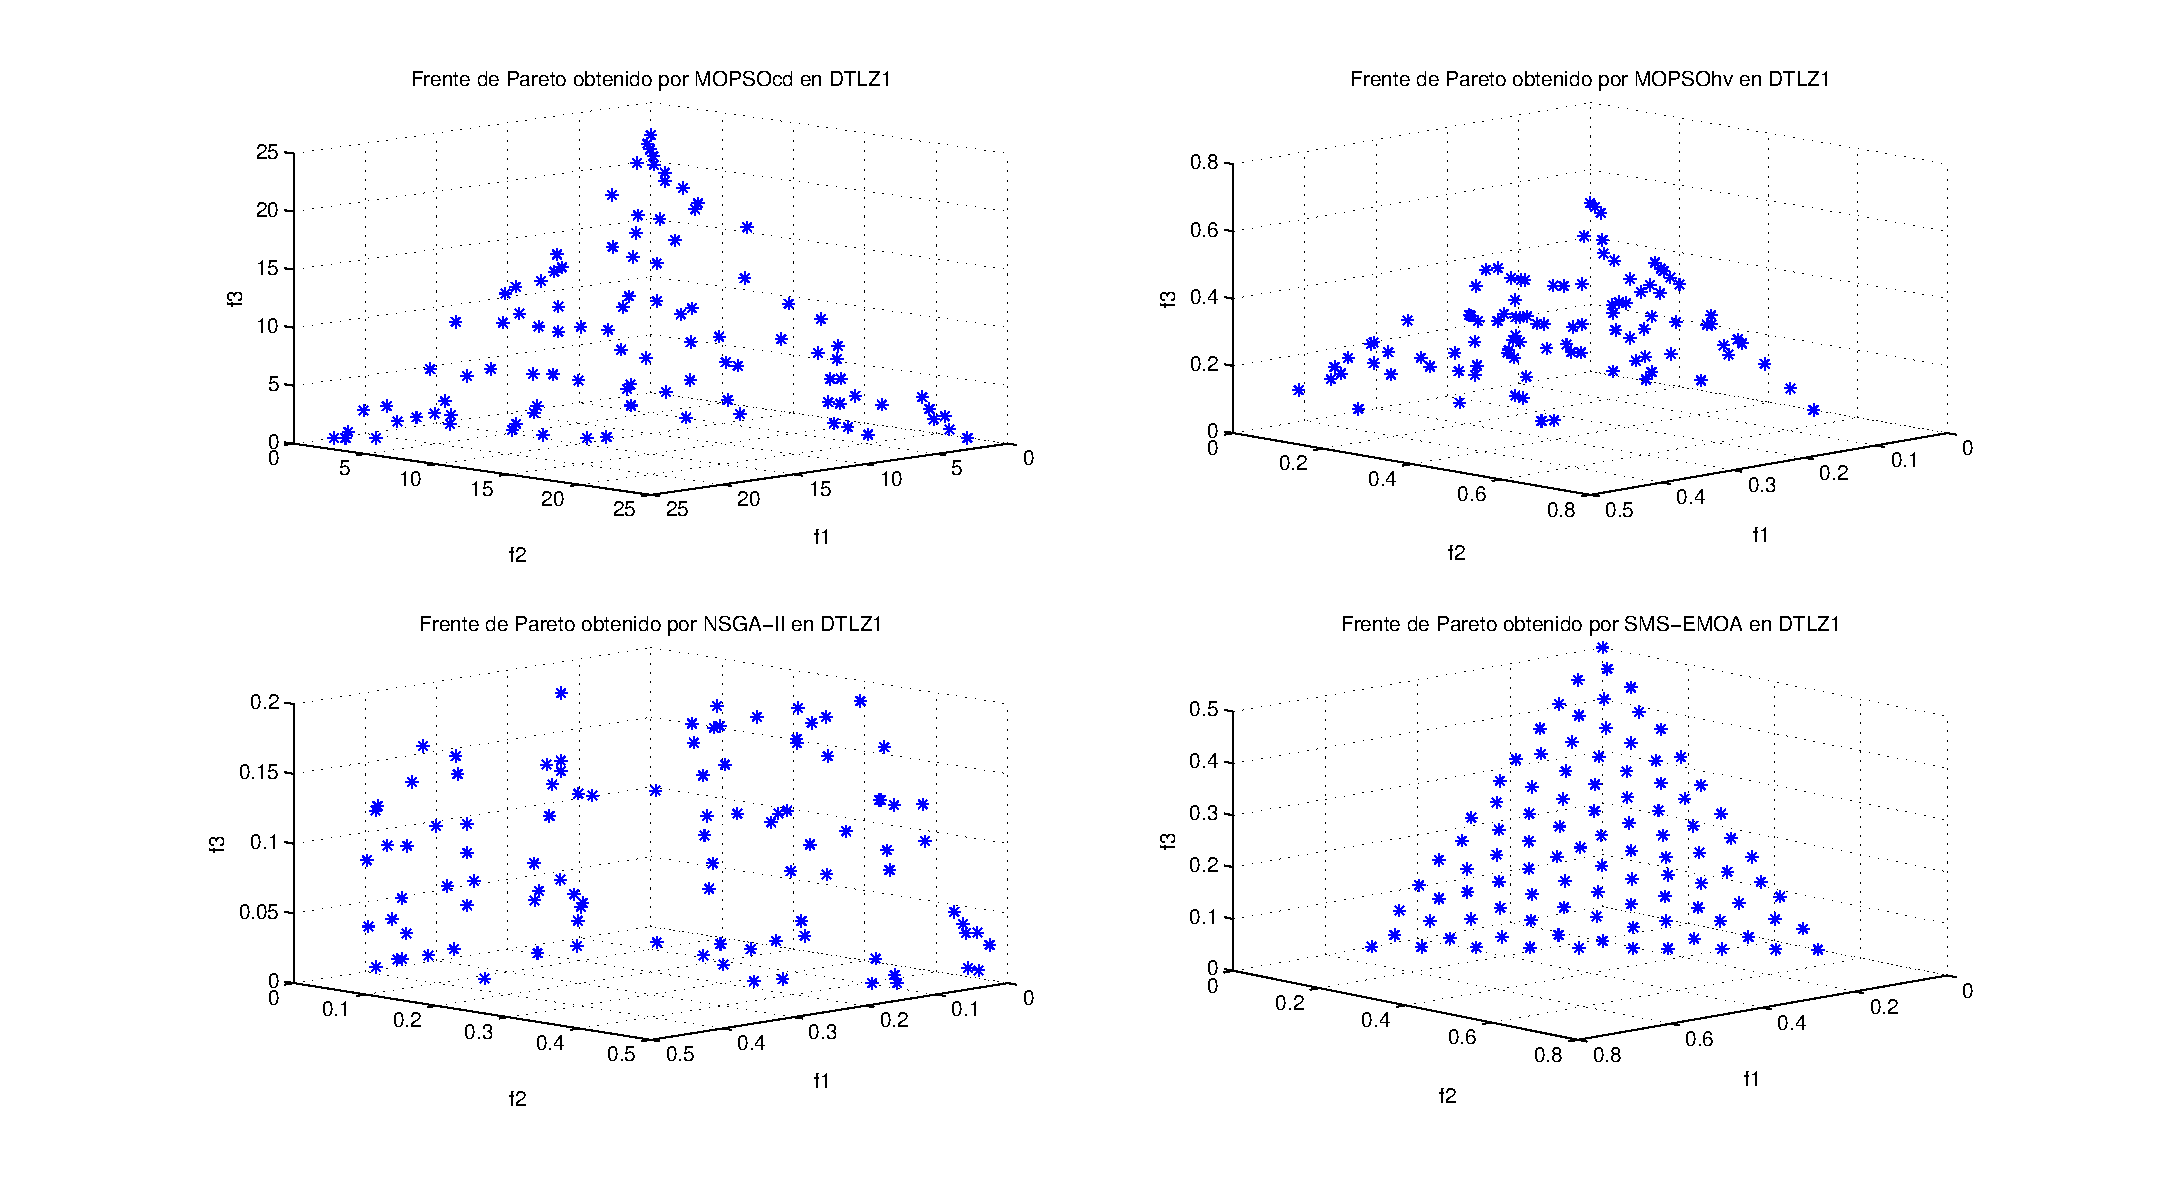
\includegraphics[scale=0.45]{Cap4/rdtlz1r.eps}
      \end{center}
	\caption{Resultados gr\'aficos correspondientes al problema DTLZ1.}
      \label{fig:rDTLZ1}
\end{figure}

\clearpage
\newpage

\begin{table}
 \begin{center}
  \begin{tabular}{|l|cc|cc|} \hline
    & \multicolumn{4}{|c|}{Espaciado} \\ 
	\textbf{Algoritmo} & \textbf{Menor} & \textbf{Mayor} & \textbf{Promedio} & \textbf{Desviaci\'on} \\  \hline \hline
	MOPSOhv &0.031912 & 0.087823 &  \textbf{\textcolor{red}{0.056173}} &  \textbf{\textcolor{red}{ 0.012780}}    \\ 
	MOPSOcd &0.042795 & 0.064965 &  \textbf{\textcolor{blue}{0.052077}} &  \textbf{\textcolor{green}{0.005154}}  \\ 
	NSGA-II &0.043968 & 0.065239 &  \textbf{\textcolor{green}{0.055460}} &  \textbf{\textcolor{blue}{0.005003}}   \\  
	SMS-EMOA &0.040210 & 0.047397 & \textbf{0.042716} &  \textbf{0.001942 }  \\  
	\hline\hline
    & \multicolumn{4}{|c|}{DGI} \\ 
	\hline\hline
	MOPSOhv &0.000421 & 0.003117 &  \textbf{\textcolor{green}{0.000806}} &  \textbf{\textcolor{green}{0.000611}}    \\ 
	MOPSOcd &0.000353 & 0.000430 & \textbf{0.000383} & \textbf{\textcolor{red}{ 0.000022}}   \\ 
	NSGA-II &0.000354 & 0.000437 &  \textbf{\textcolor{blue}{0.000380}} &  \textbf{\textcolor{blue}{0.000018}}   \\  
	SMS-EMOA &0.005000 & 0.005000 &  \textbf{\textcolor{red}{0.005000}} &  \textbf{0.000000}   \\  
	\hline\hline
    & \multicolumn{4}{|c|}{Hipervolumen} \\ 
	\hline \hline
	MOPSOhv &0.477781 & 0.695914 &  \textbf{\textcolor{red}{0.626972}} &  \textbf{\textcolor{red}{0.046583}}   \\ 
	MOPSOcd &0.637661 & 0.700693 &  \textbf{\textcolor{green}{0.669615}} &  \textbf{\textcolor{green}{0.019100}}   \\ 
	NSGA-II &0.676094 & 0.709199 &  \textbf{\textcolor{blue}{0.697212}} &  \textbf{\textcolor{blue}{0.007736}}   \\  
	SMS-EMOA &0.757997 & 0.758163 & \textbf{0.758091} &  \textbf{0.000047 }  \\  
	\hline\hline
	& \multicolumn{4}{|c|}{\textbf{Cobertura}} \\ \hline\hline 
	\textbf{Algoritmo} & \textbf{MOPSOhv} & \textbf{MOPSOcd} & \textbf{NSGA-II} & \textbf{SMS-EMOA} \\  \hline \hline
	\textbf{MOPSOhv} & ---       & \textbf{0.225500}  &  \textbf{0.009000} &  \textbf{\textcolor{red}{0.000000}} \\ 
	\textbf{MOPSOcd} &  0.000000 & ---       & 0.001500  & 0.000000  \\ 
	\textbf{NSGA-II} & 0.001000  &  0.296000 & ---       & 0.010000 \\  
	\textbf{SMS-EMOA}& \textbf{0.003000}  & 0.444000  &  0.006000 & --- \\  
	\hline
	\end{tabular}
\caption{Resultados correspondientes al problema DTLZ2.}
  \label{tab:dtlz2}
\end{center}
\end{table}

En el problema DTLZ2 se observa que en nuestra propuesta (MOPSOhv) no tiene una distribuci\'on de las soluciones, lo que causa que existan espacios grandes
en la aproximaci\'on al frente de Pareto, como se observa en la figura \ref{fig:rDTLZ2}, lo que causa que no se tenga una mayor cobertura 
del frente de Pareto, por lo tanto, el valor de la m\'etrica del hipervolumen disminuya, como se observa en la tabla \ref{tab:dtlz2}. Esto se 
debe, a que nuestra propuesta utiliza una m\'etrica que aproxima las contribuciones al hipervolumen para reemplazar soluciones en el archivo, 
por lo que, disminuye la calidad de las soluciones alcanzadas por \'este. Nuestra propuesta es superada por el SMS-EMOA y 
NSGA-II y conforme a estos resultados se puede crear una jerarqu\'ia en orden descendente en t\'erminos de convergencia del conjunto de 
soluciones pr\'oximas al frente de Pareto real:


\begin{enumerate}
  \item SMS-EMOA
  \item NSGA-II
  \item MOPSOhv
  \item MOPSOcd
\end{enumerate}

Tambi\'en, se observa que en las soluciones de nuestra propuesta dominan a las soluciones del NSGA-II y MOPSOcd, y siendo superado por las 
soluciones del SMS-EMOA.
\clearpage
\newpage

\begin{figure}
      \begin{center}
	  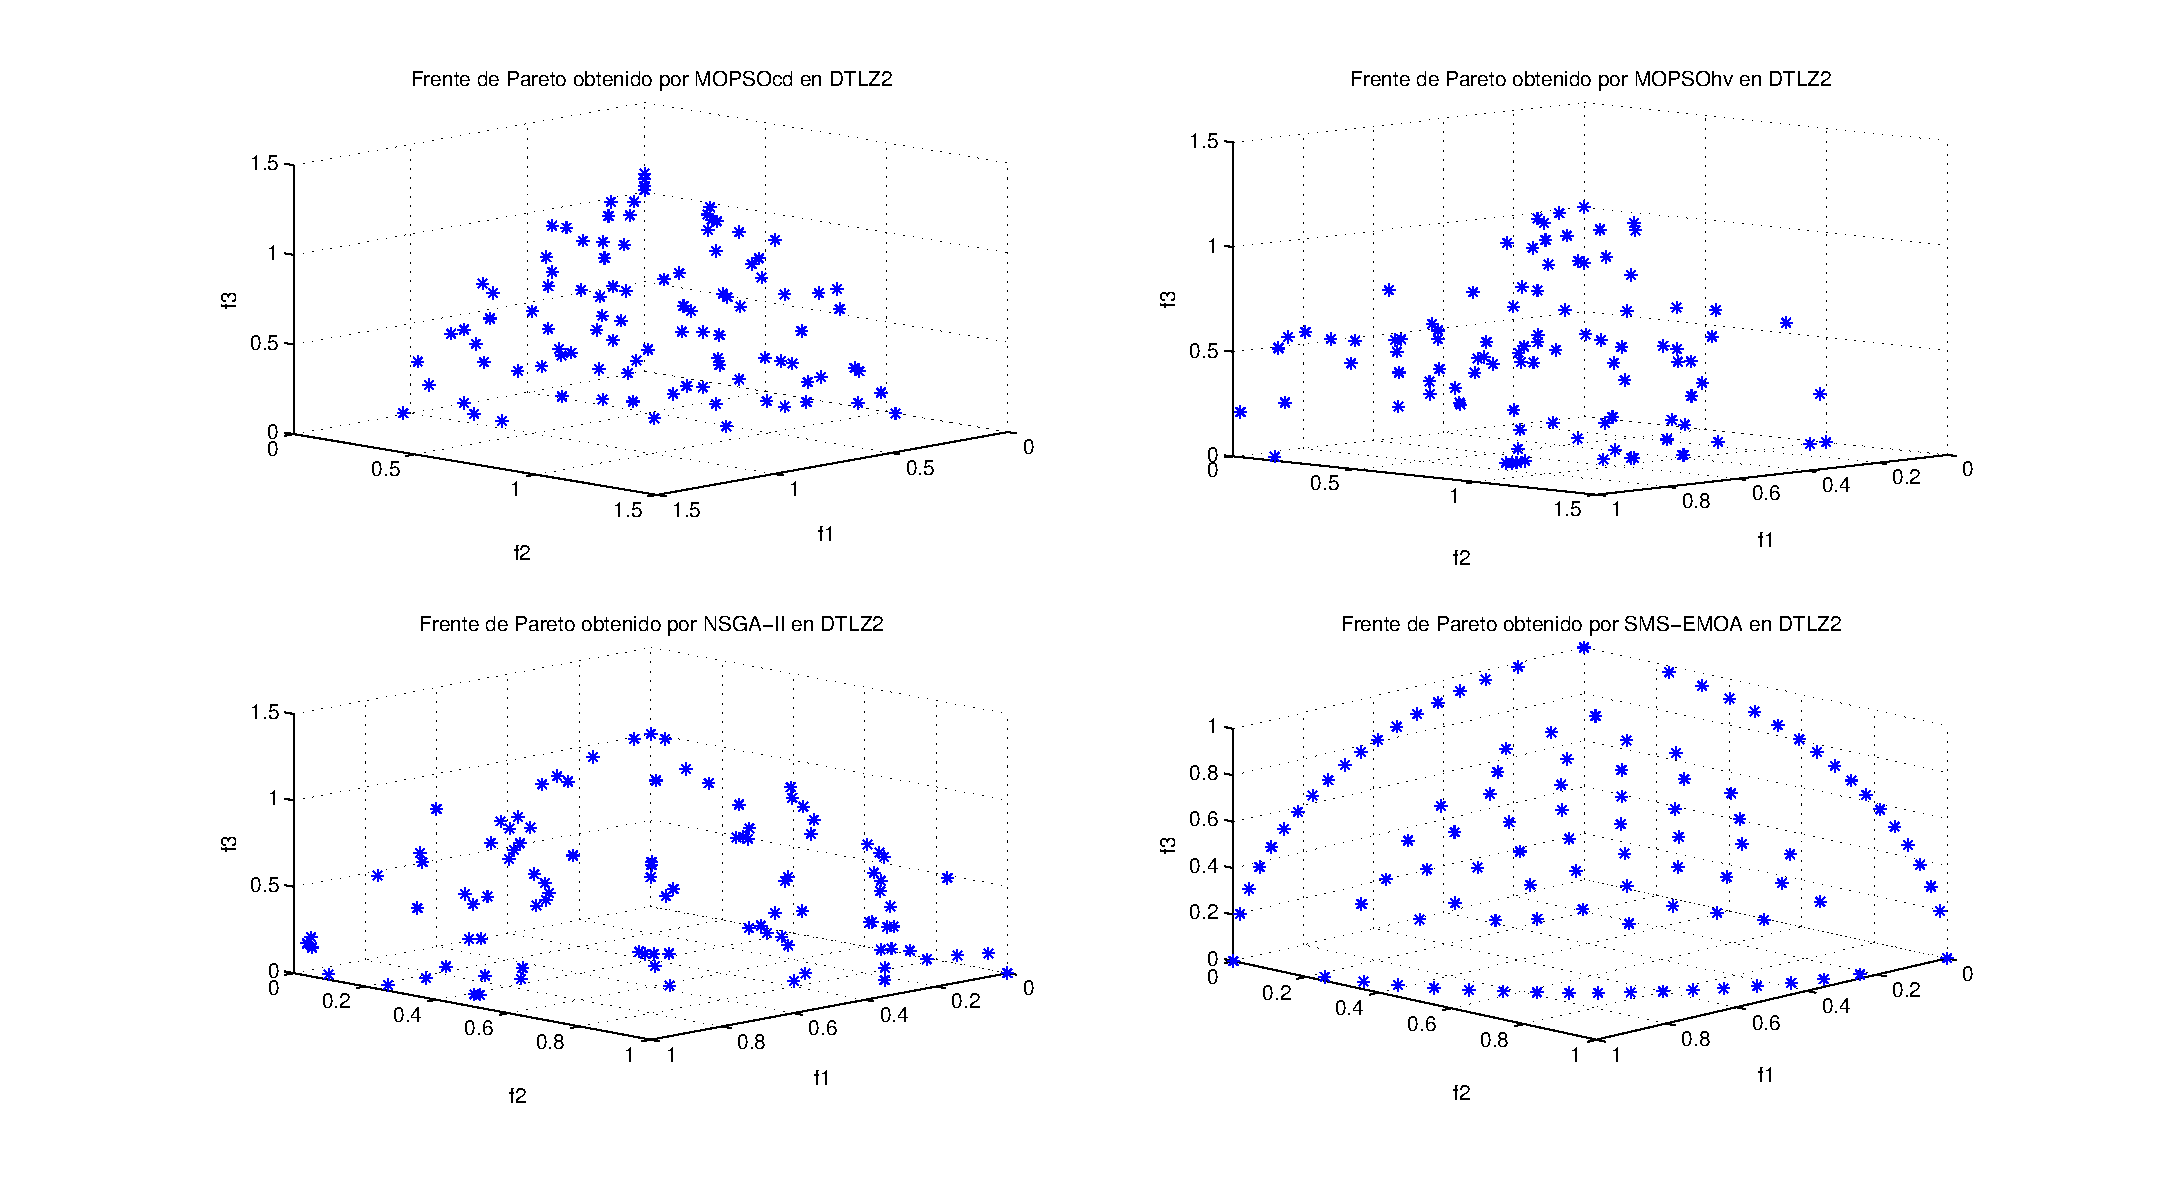
\includegraphics[scale=0.45]{Cap4/rdtlz2r.eps}
      \end{center}
	\caption{Resultados gr\'aficos correspondientes al problema DTLZ2.}
      \label{fig:rDTLZ2}
      \end{figure}

      \clearpage
      \newpage
 
\begin{table}
 \begin{center}
  \begin{tabular}{|l|cc|cc|} \hline
    & \multicolumn{4}{|c|}{Espaciado} \\ 
	\textbf{Algoritmo} & \textbf{Menor} & \textbf{Mayor} & \textbf{Promedio} & \textbf{Desviaci\'on} \\  \hline \hline
	MOPSOhv &0.523852 & 6.539527 & \textbf{\textcolor{green}{ 1.759328}} &  \textbf{\textcolor{red}{1.322038}}    \\ 
	MOPSOcd &0.774392 & 5.346362 & \textbf{\textcolor{red}{ 2.143857}} &  \textbf{\textcolor{green}{0.915538}}   \\ 
	NSGA-II &0.045404 & 0.067297 & \textbf{\textcolor{blue}{ 0.056032}} &  \textbf{0.004531}   \\  
	SMS-EMOA &0.037710 & 0.083937 & \textbf{0.043889} & \textbf{\textcolor{blue}{ 0.009394 }} \\  
	\hline\hline
    & \multicolumn{4}{|c|}{DGI} \\ 
	\hline\hline
	MOPSOhv &0.187750 & 1.484958 & \textbf{\textcolor{green}{ 0.594644}} &  \textbf{\textcolor{green}{0.302257}}   \\ 
	MOPSOcd &0.199480 & 1.812156 & \textbf{\textcolor{red}{ 0.630432}} & \textbf{\textcolor{red}{ 0.323953}}  \\ 
	NSGA-II &0.001123 & 0.001441 & \textbf{0.001235} &  \textbf{0.000083} \\  
	SMS-EMOA &0.015616 & 0.031270 & \textbf{\textcolor{blue}{ 0.016425}} &  \textbf{\textcolor{blue}{0.003406}}  \\  
	\hline\hline
    & \multicolumn{4}{|c|}{Hipervolumen} \\ 
	\hline\hline
	MOPSOhv &0.000000 & 0.000000 & \textbf{\textcolor{green}{ 0.000000 }}& \textbf{\textcolor{green}{ 0.000000 }}\\ 
	MOPSOcd &0.000000 & 0.000000 &  \textbf{\textcolor{red}{0.000000}} & \textbf{\textcolor{red}{ 0.000000 }} \\ 
	NSGA-II &123.004398 & 124.174476 &  \textbf{\textcolor{blue}{123.673815}} &  \textbf{0.295556} \\  
	SMS-EMOA &120.390195 & 124.425951 & \textbf{124.221079} & \textbf{\textcolor{blue}{ 0.878873}}  \\  
	\hline\hline
	& \multicolumn{4}{|c|}{\textbf{Cobertura}} \\ \hline\hline 
	\textbf{Algoritmo} & \textbf{MOPSOhv} & \textbf{MOPSOcd} & \textbf{NSGA-II} & \textbf{SMS-EMOA} \\  \hline \hline
	\textbf{MOPSOhv} &---       & \textbf{0.546000} & \textbf{\textcolor{red}{ 0.000000 }}  &  \textbf{\textcolor{red}{0.000000 }} \\ 
	\textbf{MOPSOcd} & 0.215500 & ---      & 0.000000 & 0.000000 \\ 
	\textbf{NSGA-II} & \textbf{1.000000} & 0.980000 & ---        & 0.052000 \\  
	\textbf{SMS-EMOA}& \textbf{0.960000} & 0.940000 & 0.000000   & --- \\  
	\hline
	\end{tabular}
\caption{Resultados correspondientes al problema DTLZ3.}
  \label{tab:dtlz3}
\end{center}
\end{table}
La multimodalidad de DTLZ3 causa dificultad a nuestra propuesta (MOPSOhv) para converger de manera \'optima, como se muestra en la 
tabla \ref{tab:dtlz3}. En la gr\'afica \ref{fig:rDTLZ3} se muestra que el MOPSOcd y nuestra propuesta no tiene una buena convergencia
al frente de Pareto y no muestran una buena distribuci\'on de las soluciones. Sin embargo, nuestra propuesta domina a las soluciones 
del MOPSOcd. Nuestra propuesta es superada por el SMS-EMOA y NSGA-II y conforme a estos resultados se puede crear una
jerarqu\'ia en orden descendente en t\'erminos de convergencia del conjunto de soluciones pr\'oximas al frente de Pareto real:

\begin{enumerate}
  \item NSGA-II
  \item SMS-EMOA
  \item MOPSOhv
  \item MOPSOcd
\end{enumerate}

\clearpage
\newpage

\begin{figure}
      \begin{center}
	  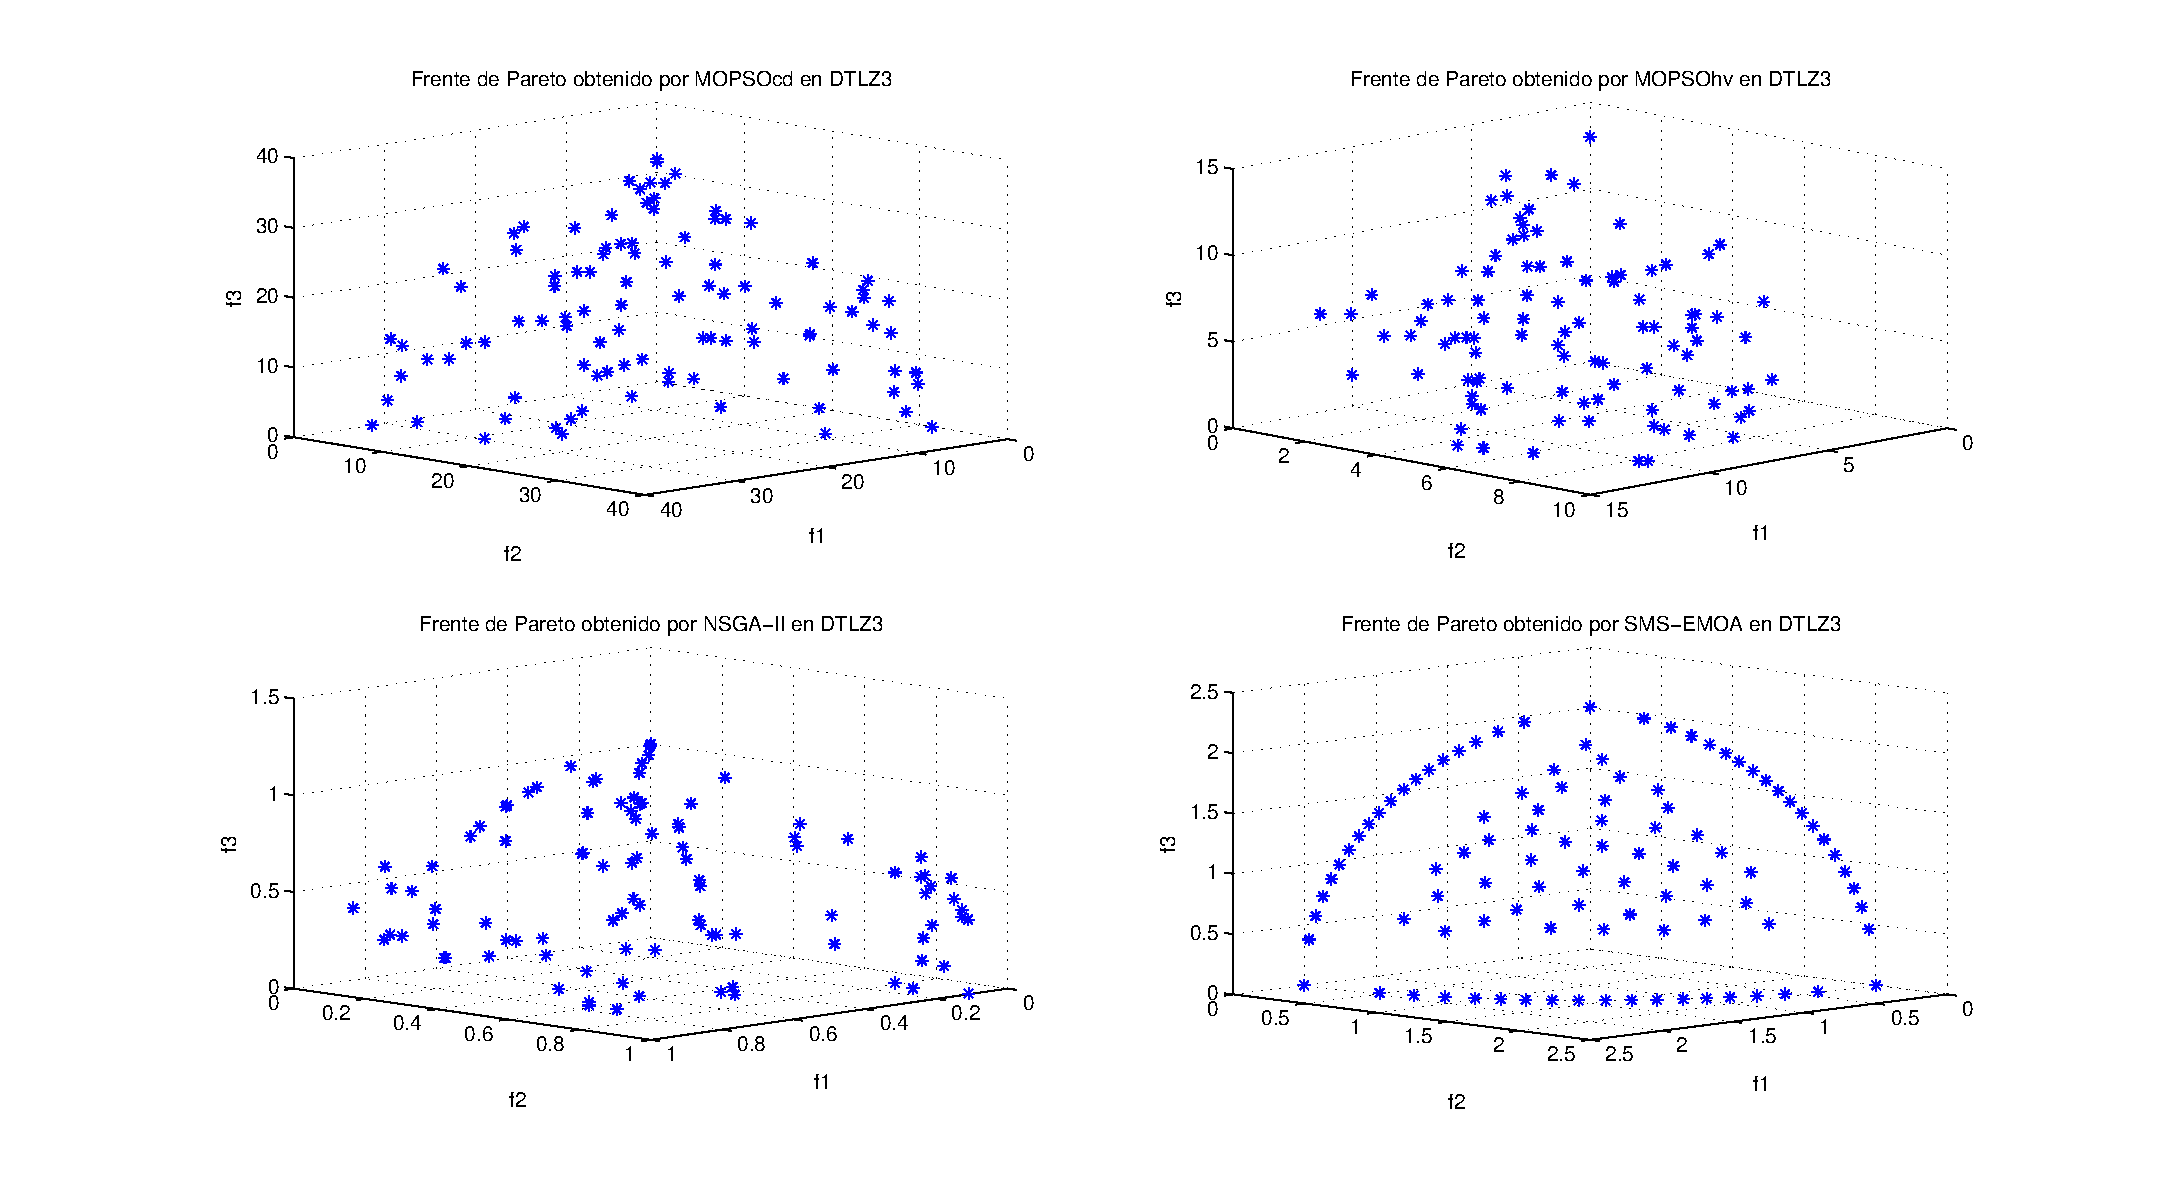
\includegraphics[scale=0.45]{Cap4/rdtlz3r.eps}
      \end{center}
	\caption{Resultados gr\'aficos correspondientes al problema DTLZ3.}
      \label{fig:rDTLZ3}
      \end{figure}

      \clearpage
      \newpage
 

\begin{table}
 \begin{center}
  \begin{tabular}{|l|cc|cc|} \hline
    & \multicolumn{4}{|c|}{Espaciado} \\ 
	\textbf{Algoritmo} & \textbf{Menor} & \textbf{Mayor} & \textbf{Promedio} & \textbf{Desviaci\'on} \\  \hline \hline
	MOPSOhv &0.009443 & 0.080015 & \textbf{\textcolor{blue}{ 0.047999}} & \textbf{\textcolor{red}{ 0.021016}}    \\ 
	MOPSOcd &0.052363 & 0.061539 & \textbf{\textcolor{red}{ 0.056542}} & \textbf{\textcolor{blue}{ 0.002922}}  \\ 
	NSGA-II &0.000000 & 0.063012 &  \textbf{\textcolor{green}{0.051862}} & \textbf{\textcolor{green}{ 0.013087}}   \\  
	SMS-EMOA & 0.039215 & 0.045833 & \textbf{0.042030} & \textbf{ 0.001928}   \\  
	\hline\hline
    & \multicolumn{4}{|c|}{DGI} \\ 
	\hline\hline
	MOPSOhv &0.003982 & 0.010549 &  \textbf{\textcolor{green}{0.006694}} &  \textbf{\textcolor{green}{0.002366}}   \\ 
	MOPSOcd &0.001142 & 0.001271 & \textbf{0.001208} & \textbf{\textcolor{blue}{ 0.000037}} \\ 
	NSGA-II &0.001097 & 0.015257 &  \textbf{\textcolor{blue}{0.001875}} & \textbf{\textcolor{red}{ 0.003071}}   \\  
	SMS-EMOA &0.015606 & 0.015606 & \textbf{\textcolor{red}{0.015606}} &  \textbf{0.000000}   \\  
	\hline\hline
    & \multicolumn{4}{|c|}{Hipervolumen} \\ 
	\hline \hline
	MOPSOhv &0.337305 & 0.666145 &  \textbf{\textcolor{red}{0.548703}} & \textbf{\textcolor{green}{0.117426}} \\ 
	MOPSOcd &0.668445 & 0.708459 &  \textbf{\textcolor{blue}{0.688920}} & \textbf{\textcolor{blue}{ 0.010033}}  \\ 
	NSGA-II &0.121000 & 0.715370 & \textbf{\textcolor{green}{ 0.674632}} & \textbf{\textcolor{red}{ 0.127135}}  \\  
	SMS-EMOA &0.757966 & 0.758160 &\textbf{ 0.758069} & \textbf{0.000050}   \\  
	\hline\hline
	& \multicolumn{4}{|c|}{\textbf{Cobertura}} \\ \hline\hline 
	\textbf{Algoritmo} & \textbf{MOPSOhv} & \textbf{MOPSOcd} & \textbf{NSGA-II} & \textbf{SMS-EMOA} \\  \hline \hline
	\textbf{MOPSOhv} &---       & \textbf{0.189000}   & \textbf{0.013500}   &  \textbf{0.017000} \\ 
	\textbf{MOPSOcd} & 0.000000  & ---       & 0.000500   &  0.000000   \\ 
	\textbf{NSGA-II} & 0.008421  & 0.199500  & ---       &  0.000000  \\  
	\textbf{SMS-EMOA}&  0.000000 & 0.275500  & 0.009500 & --- \\  
	\hline
	\end{tabular}
\caption{Resultados correspondientes al problema DTLZ4.}
  \label{tab:dtlz4}
\end{center}
\end{table}
En el problema DTLZ4 se observa que en las soluciones de nuestra propuesta (MOPSOhv) la distribuci\'on de las soluciones se concentren
en los extremos, causando que existan espacios muy grandes en el centro del frente de Pareto, como se observa en la 
figura \ref{fig:rDTLZ4}, y como consecuencia  el valor de la m\'etrica del hipervolumen disminuya, como se observa en la tabla \ref{tab:dtlz4}. 
Esto puede ser por que nuestra propuesta se concentra en los extremos del frente, ya que estos, pueden
ser aquellas part\'iculas que gu\'ian la b\'usqueda de nuevas solciones, seg\'un su contribuci\'on al hipervolumen. Nuestra propuesta es superada 
por el SMS-EMOA y NSGA-II y conforme a estos resultados se puede crear una jerarqu\'ia en orden descendente en t\'erminos de convergencia del conjunto de 
soluciones pr\'oximas al frente de Pareto real:


\begin{enumerate}
  \item SMS-EMOA
  \item NSGA-II
  \item MOPSOhv
  \item MOPSOcd
\end{enumerate}

Tambi\'en, se observa que en las soluciones de nuestra propuesta dominan a las soluciones de los otros algoritmos.
\clearpage
\newpage

\begin{figure}
      \begin{center}
	  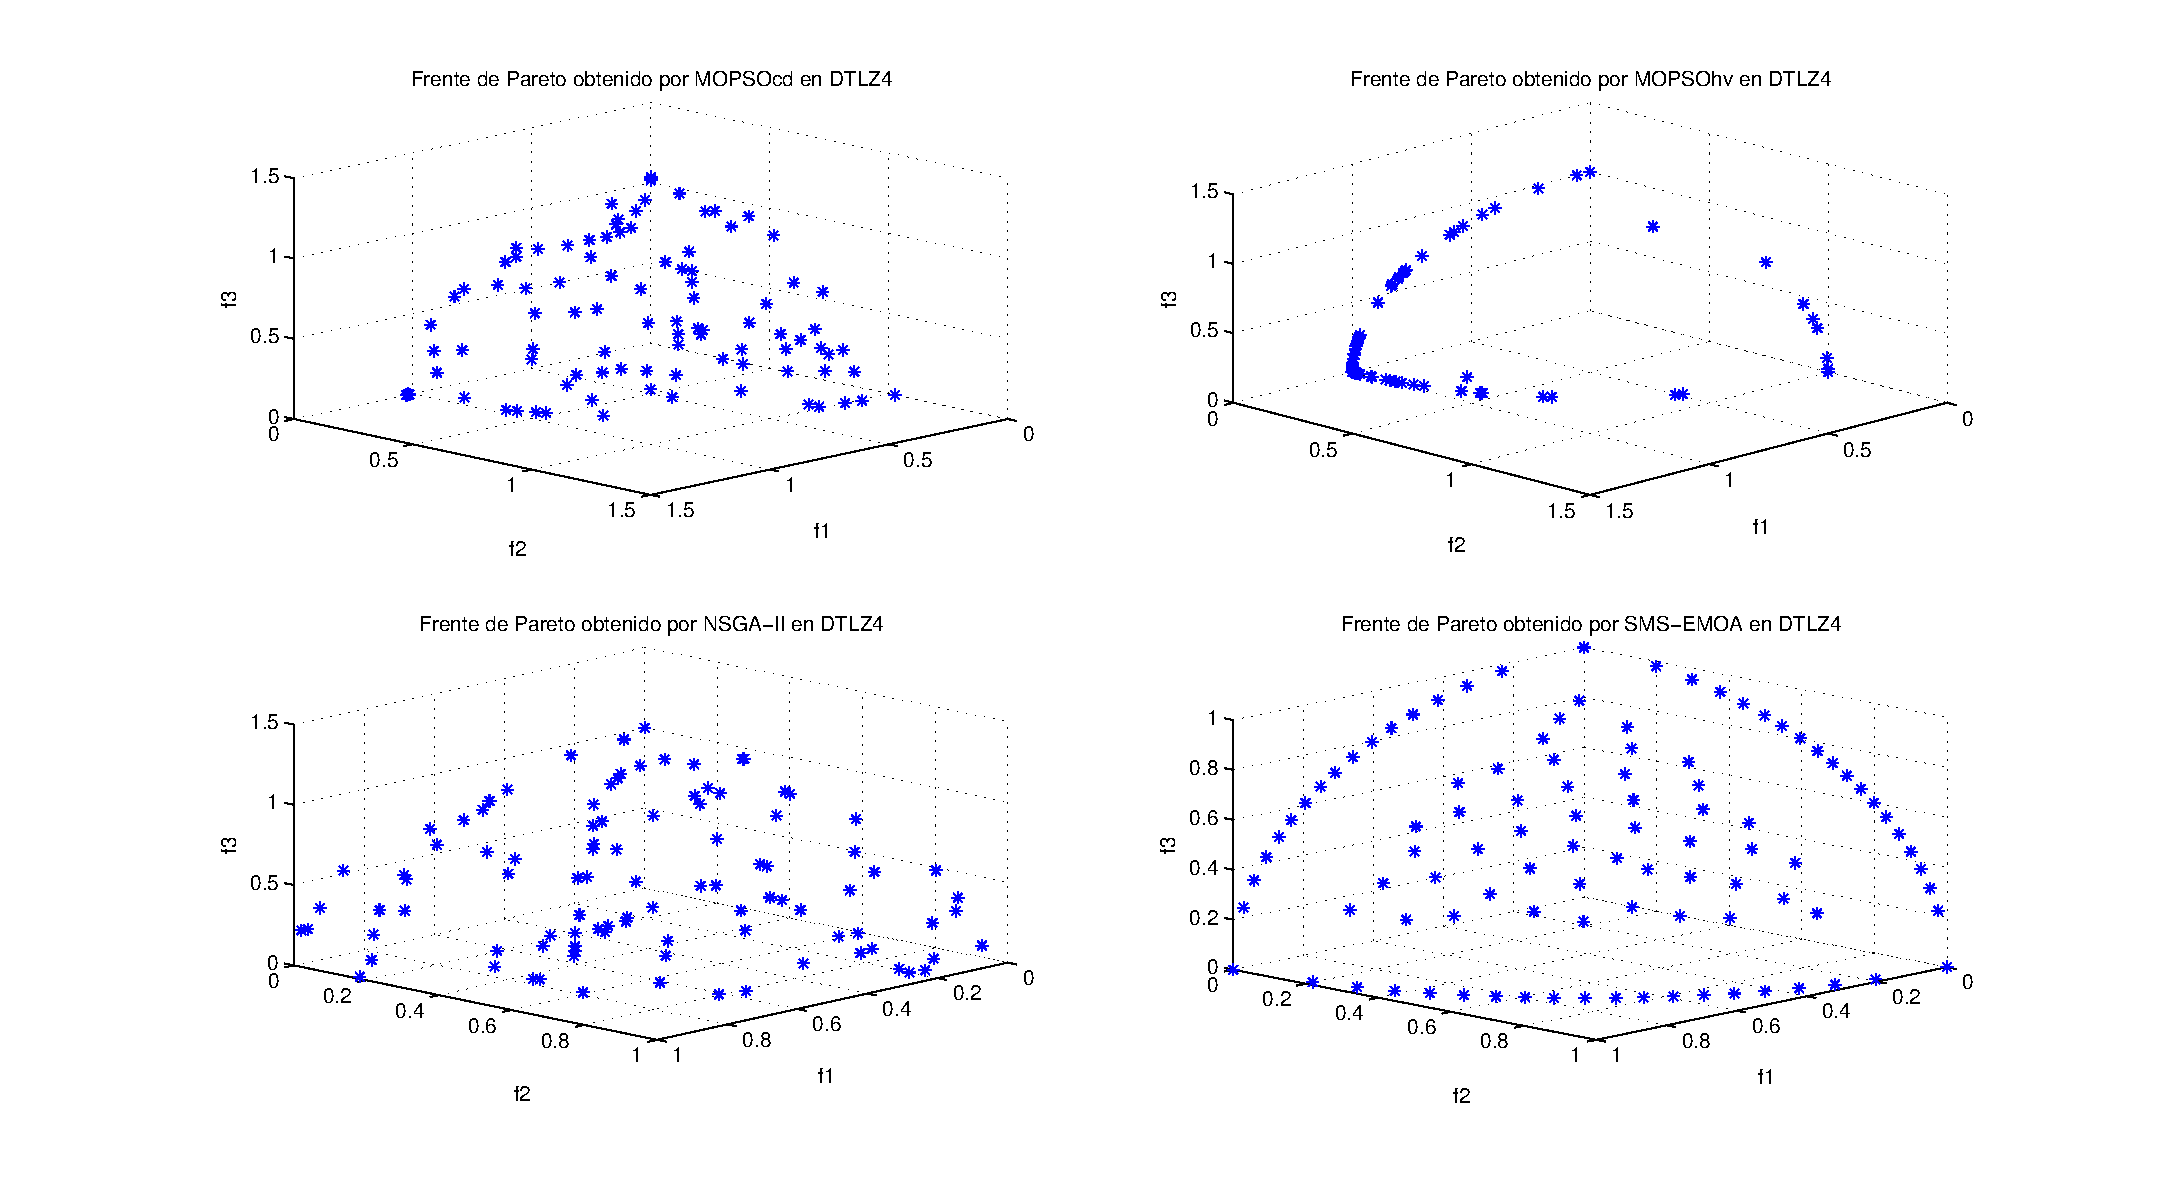
\includegraphics[scale=0.45]{Cap4/rdtlz4r.eps}
      \end{center}
	\caption{Resultados gr\'aficos correspondientes al problema DTLZ4.}
      \label{fig:rDTLZ4}
   \end{figure}

   \clearpage
   \newpage

\begin{table}
 \begin{center}
  \begin{tabular}{|l|cc|cc|} \hline
    & \multicolumn{4}{|c|}{Espaciado} \\ 
	\textbf{Algoritmo} & \textbf{Menor} & \textbf{Mayor} & \textbf{Promedio} & \textbf{Desviaci\'on} \\  \hline \hline
	MOPSOhv &0.009066 & 0.027088 &  \textbf{\textcolor{red}{0.016552}} &  \textbf{\textcolor{blue}{0.005419}}   \\ 
	MOPSOcd &0.007105 & 0.009411 & \textbf{0.008436} & \textbf{\textcolor{green}{ 0.000610 }}  \\ 
	NSGA-II &0.008281 & 0.011557 &  \textbf{\textcolor{green}{0.009727}} &  \textbf{\textcolor{red}{0.000757}}  \\  
	SMS-EMOA &0.008044 & 0.009672 &  \textbf{\textcolor{blue}{0.008763}} &  \textbf{0.000463}  \\  
	\hline\hline
    & \multicolumn{4}{|c|}{DGI} \\ 
	\hline\hline
	MOPSOhv &0.000125 & 0.001589 &  \textbf{\textcolor{green}{0.000439}} & \textbf{\textcolor{red}{ 0.000390}}   \\ 
	MOPSOcd &0.000049 & 0.000058 & \textbf{0.000054} &  \textbf{\textcolor{blue}{0.000002}} \\ 
	NSGA-II &0.000061 & 0.000083 &  \textbf{\textcolor{blue}{0.000069}} &  \textbf{\textcolor{green}{0.000005}}   \\  
	SMS-EMOA &0.009901 & 0.009901 & \textbf{\textcolor{red}{ 0.009901}} &  \textbf{0.000000}   \\  
	\hline
    & \multicolumn{4}{|c|}{Hipervolumen} \\ 
	\hline\hline
	MOPSOhv &0.396024 & 0.435369 &  \textbf{\textcolor{red}{0.428426}} &  \textbf{\textcolor{red}{0.010028}}   \\ 
	MOPSOcd &0.438762 & 0.438946 & \textbf{\textcolor{blue}{0.438852}} &  \textbf{\textcolor{blue}{0.000056}}  \\ 
	NSGA-II &0.437414 & 0.438274 &  \textbf{\textcolor{green}{0.437990}} &  \textbf{\textcolor{green}{0.000223}}  \\  
	SMS-EMOA &0.439348 & 0.439390 & \textbf{0.439374} & \textbf{0.000011}   \\  
	\hline\hline
	& \multicolumn{4}{|c|}{\textbf{Cobertura}} \\ \hline\hline 
	\textbf{Algoritmo} & \textbf{MOPSOhv} & \textbf{MOPSOcd} & \textbf{NSGA-II} & \textbf{SMS-EMOA} \\  \hline \hline
	\textbf{MOPSOhv} &---       & \textbf{0.024500}   &   \textbf{0.024500}  &   \textbf{\textcolor{red}{0.000000}}   \\ 
	\textbf{MOPSOcd} & 0.006500 & ---        &  0.034500 &  0.010000 \\ 
	\textbf{NSGA-II} & 0.020500 &  0.000000  & ---       & 0.010000  \\  
	\textbf{SMS-EMOA}& \textbf{0.000500} &  0.000000  & 0.022000  & --- \\  
	\hline

	\end{tabular}
\caption{Resultados correspondientes al problema DTLZ5.}
  \label{tab:dtlz5}
\end{center}
\end{table}

En el problema DTLZ5 se observa que en nuestra propuesta (MOPSOhv) no tiene una distribuci\'on de las soluciones, lo que causa que existan 
espacios en la aproximaci\'on al frente de Pareto, como se observa en la figura \ref{fig:rDTLZ2}, lo que causa que no se tenga una buena 
cobertura del frente de Pareto, por lo tanto, el valor de la m\'etrica del hipervolumen disminuya, como se observa en la tabla \ref{tab:dtlz2}. 
Nuestra propuesta es superada por el SMS-EMOA y NSGA-II y conforme a estos resultados se puede crear una jerarqu\'ia en orden descendente en t\'erminos de convergencia del conjunto de 
soluciones pr\'oximas al frente de Pareto real:


\begin{enumerate}
  \item NSGA-II
  \item SMS-EMOA
  \item MOPSOcd
  \item MOPSOhv
\end{enumerate}

Tambi\'en, se observa que en las soluciones de nuestra propuesta dominan a las soluciones del NSGA-II y MOPSOcd, y siendo superado por las 
soluciones del SMS-EMOA.

\clearpage
\newpage
 \begin{figure}
      \begin{center}
	  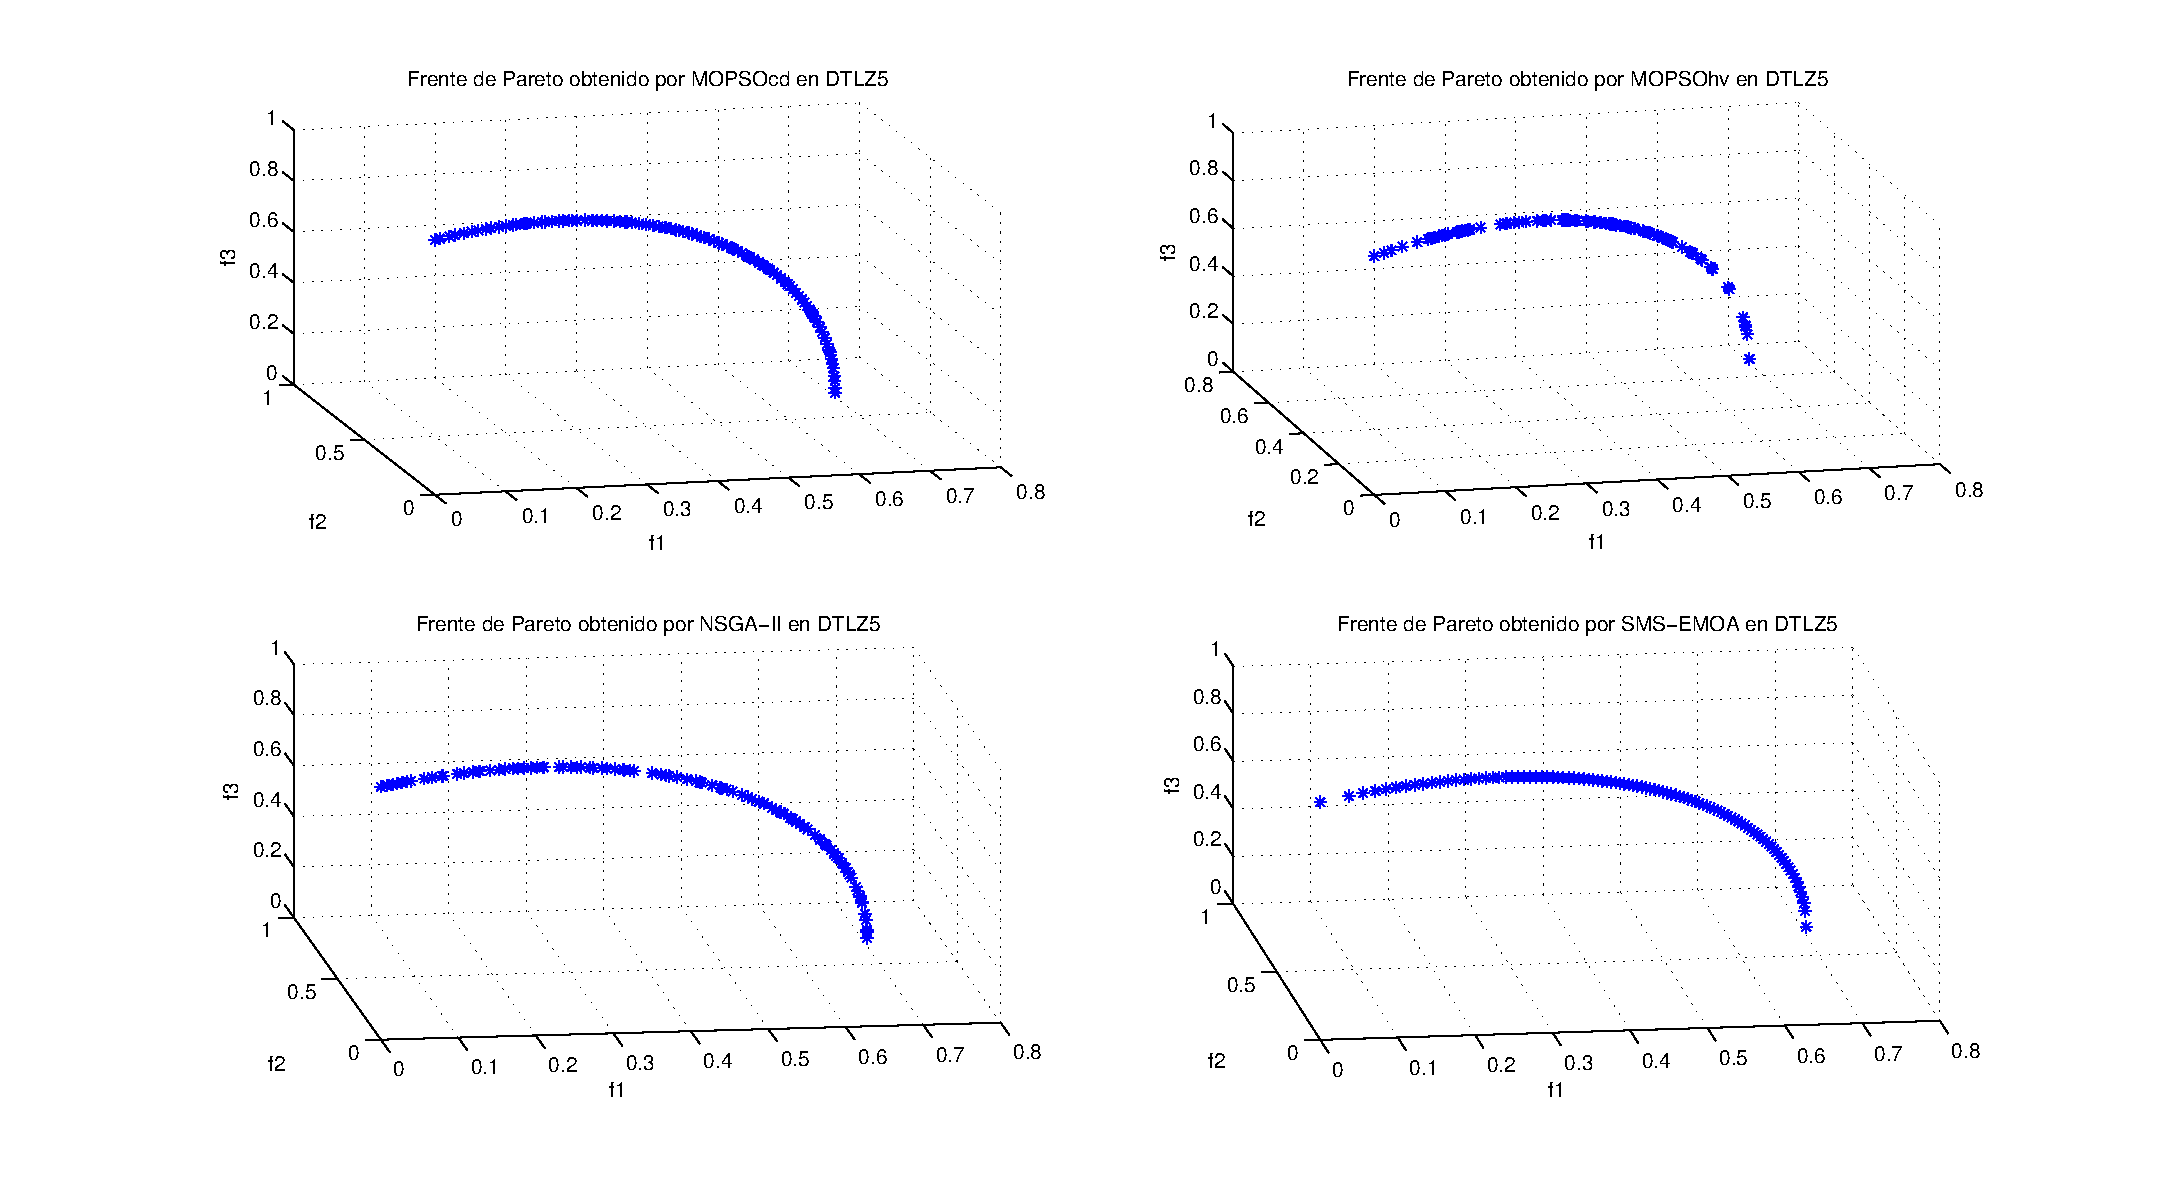
\includegraphics[scale=0.45]{Cap4/rdtlz5r.eps}
      \end{center}
	\caption{Resultados gr\'aficos correspondientes al problema DTLZ5.}
      \label{fig:rDTLZ5}
 \end{figure}
\clearpage
 \newpage
\begin{table}
 \begin{center}
  \begin{tabular}{|l|cc|cc|} \hline
    & \multicolumn{4}{|c|}{Espaciado} \\ 
	\textbf{Algoritmo} & \textbf{Menor} & \textbf{Mayor} & \textbf{Promedio} & \textbf{Desviaci\'on} \\  \hline \hline
	MOPSOhv &0.128037 & 0.220886 &  \textbf{\textcolor{red}{0.158278}} & \textbf{\textcolor{green}{ 0.026187}}   \\ 
	MOPSOcd &0.271101 & 0.501514 &  \textbf{\textcolor{green}{0.343938}} & \textbf{\textcolor{red}{ 0.052728}}   \\ 
	NSGA-II &0.011479 & 0.029482 & \textbf{\textcolor{blue}{ 0.020970}} &  \textbf{\textcolor{blue}{0.004354}}   \\  
	SMS-EMOA & 0.009705 & 0.020519 & \textbf{0.013185} & \textbf{0.002414}  \\  
	\hline\hline
    & \multicolumn{4}{|c|}{DGI} \\ 
	\hline\hline
	MOPSOhv &0.007386 & 0.015926 & \textbf{\textcolor{blue}{ 0.009931}} & \textbf{\textcolor{green}{0.002293}}  \\ 
	MOPSOcd &0.009901 & 0.062068 & \textbf{\textcolor{red}{ 0.036889}} & \textbf{\textcolor{red}{ 0.012547}}  \\ 
	NSGA-II &0.000083 & 0.001194 & \textbf{0.000648} &  \textbf{\textcolor{blue}{0.000236 }}  \\  
	SMS-EMOA &0.010475 & 0.011392 & \textbf{\textcolor{green}{ 0.010786 }}&  \textbf{0.000231 }  \\  
	\hline\hline
    & \multicolumn{4}{|c|}{Hipervolumen} \\ 
	\hline\hline
	MOPSOhv &0.000000 & 0.000616 & \textbf{\textcolor{green}{ 0.000391 }}& \textbf{\textcolor{green}{ 0.000277  }}  \\ 
	MOPSOcd &0.000000 & 0.000000 & \textbf{\textcolor{red}{ 0.000000 }}& \textbf{\textcolor{red}{ 0.000000 }} \\ 
	NSGA-II &0.303244 & 0.437448 & \textbf{0.361529} &  \textbf{\textcolor{blue}{0.028920 }} \\  
	SMS-EMOA &0.282821 & 0.374890 & \textbf{\textcolor{blue}{ 0.340557 }}& \textbf{0.024323 } \\  
	\hline\hline
	& \multicolumn{4}{|c|}{\textbf{Cobertura}} \\ \hline\hline 
	\textbf{Algoritmo} & \textbf{MOPSOhv} & \textbf{MOPSOcd} & \textbf{NSGA-II} & \textbf{SMS-EMOA} \\  \hline \hline
	\textbf{MOPSOhv} & --- &  \textbf{0.920000}       &  \textbf{\textcolor{red}{0.000000}}  &  \textbf{\textcolor{red}{0.000000}} \\ 
	\textbf{MOPSOcd} & 0.000000 & ---       &  0.000000 &  0.000000  \\ 
	\textbf{NSGA-II} & \textbf{0.958000} & 0.996000  & ---       & 0.479500  \\  
	\textbf{SMS-EMOA}& \textbf{0.630000} &  0.640000 & 0.001500  & --- \\  
	\hline
	\end{tabular}
\caption{Resultados correspondientes al problema DTLZ6.}
  \label{tab:dtlz6}
\end{center}
\end{table}
El problema DTLZ6 es muy dificil para nuestra propuesta (MOPSOhv) y el MOPSOcd para converger de manera \'optima, como se muestra en la 
tabla \ref{tab:dtlz6} ya que no logran acerce al frente de Parto, como se muestra en la gr\'afica \ref{fig:rDTLZ6}. Sin embargo, nuestra 
propuesta domina a las soluciones del MOPSOcd. Nuestra propuesta es superada por el SMS-EMOA y NSGA-II y conforme a estos resultados se puede 
crear una jerarqu\'ia en orden descendente en t\'erminos de convergencia del conjunto de soluciones pr\'oximas al frente de Pareto real:

\begin{enumerate}
  \item NSGA-II
  \item SMS-EMOA
  \item MOPSOhv
  \item MOPSOcd
\end{enumerate}

\clearpage
\newpage
\begin{figure}
      \begin{center}
	  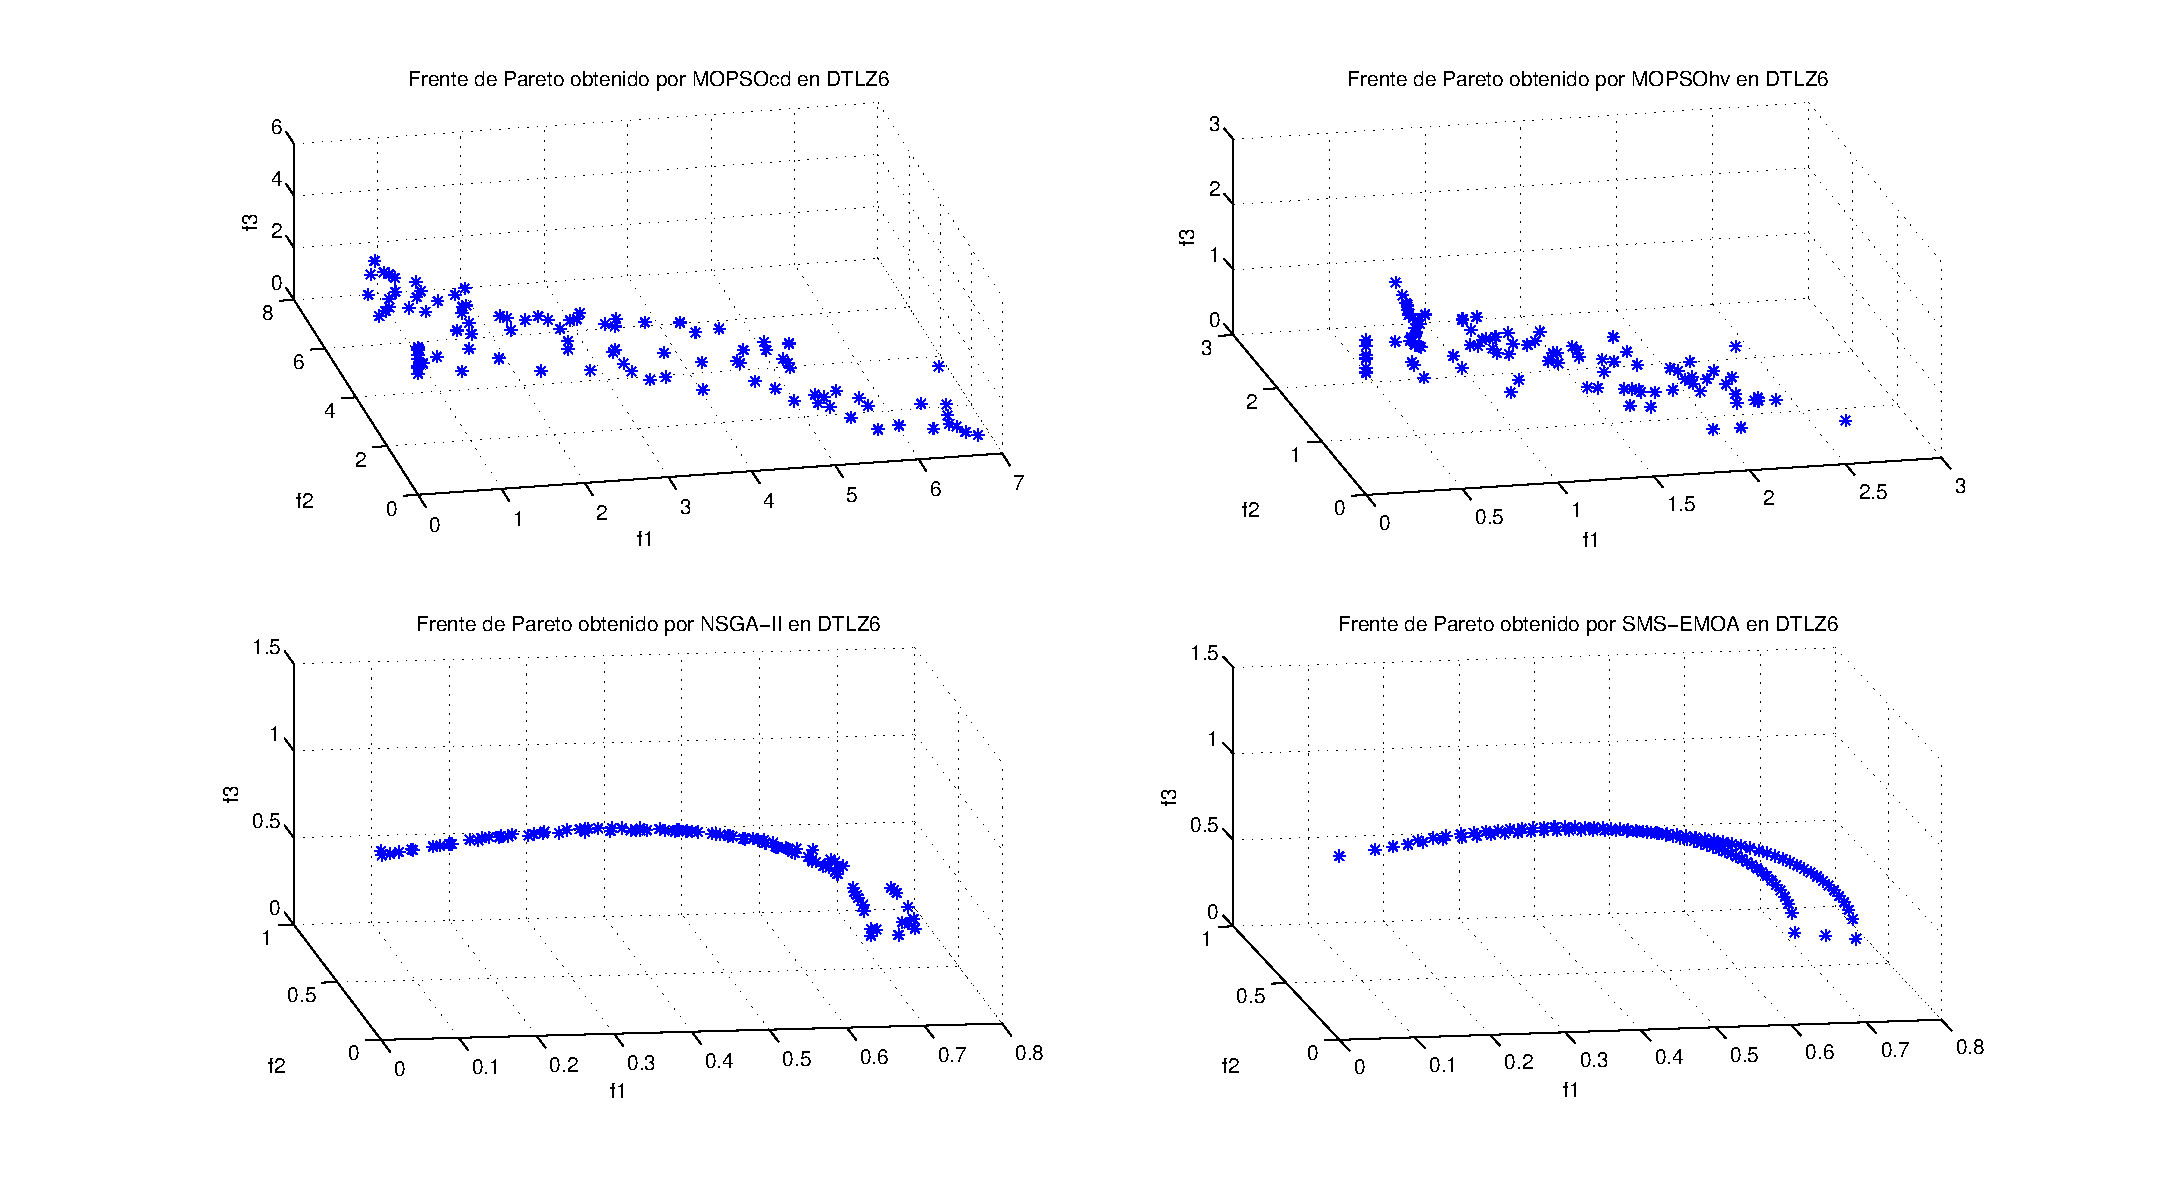
\includegraphics[scale=0.45]{Cap4/rdtlz6r.eps}
      \end{center}
	\caption{Resultados gr\'aficos correspondientes al problema DTLZ6.}
      \label{fig:rDTLZ6}
      \end{figure}
\clearpage
\newpage

 \begin{table}
 \begin{center}
 \begin{tabular}{|l|cc|cc|} \hline
    & \multicolumn{4}{|c|}{Espaciado} \\ 
	\textbf{Algoritmo} & \textbf{Menor} & \textbf{Mayor} & \textbf{Promedio} & \textbf{Desviaci\'on} \\  \hline \hline
	MOPSOhv &0.029933 & 0.140179 &  \textbf{\textcolor{green}{0.085100}} &  \textbf{\textcolor{green}{0.025882}}    \\ 
	MOPSOcd & 0.063885 & 0.453648 &  \textbf{\textcolor{red}{0.114527}} & \textbf{\textcolor{red}{0.112693}}   \\ 
	NSGA-II &0.043496 & 0.085744 &  \textbf{\textcolor{blue}{0.068548}} & \textbf{\textcolor{blue}{0.009758}}  \\  
	SMS-EMOA &0.044055 & 0.063838 & \textbf{0.057420} &  \textbf{0.005603}    \\  
	\hline
    & \multicolumn{4}{|c|}{DGI} \\ 
	\hline\hline
	MOPSOhv &0.001446 & 0.005356 &  \textbf{\textcolor{green}{0.002800}} & \textbf{\textcolor{green}{ 0.001392}}   \\ 
	MOPSOcd & 0.001228 & 0.002112 & \textbf{\textcolor{blue}{0.001558}} &  \textbf{0.000205 }  \\ 
	NSGA-II & 0.000802 & 0.005285 & \textbf{0.001123} &  \textbf{\textcolor{blue}{0.000957}}  \\  
	SMS-EMOA &0.013925 & 0.021469 &  \textbf{\textcolor{red}{0.015064}} & \textbf{\textcolor{red}{ 0.002691}}  \\  
	\hline\hline
    & \multicolumn{4}{|c|}{Hipervolumen} \\ 
	\hline\hline
	MOPSOhv & 2.359510 & 2.812829 &  \textbf{\textcolor{red}{2.608814 }}&  \textbf{\textcolor{green}{0.123164}}  \\ 
	MOPSOcd & 2.430821 & 2.744141 &  \textbf{\textcolor{green}{2.648845 }}&  \textbf{0.072522}   \\ 
	NSGA-II & 2.578211 & 3.011594 &  \textbf{\textcolor{blue}{2.974631 }}&  \textbf{\textcolor{blue}{0.091615}}   \\  
	SMS-EMOA &5.055289 & 5.528637 & \textbf{5.456793} &  \textbf{\textcolor{red}{0.168653}}   \\  
	\hline\hline	
	& \multicolumn{4}{|c|}{\textbf{Cobertura}} \\ \hline\hline 
	\textbf{Algoritmo} & \textbf{MOPSOhv} & \textbf{MOPSOcd} & \textbf{NSGA-II} & \textbf{SMS-EMOA} \\  \hline \hline
	\textbf{MOPSOhv} &---       & \textbf{0.460000}   & \textbf{0.061500} &   \textbf{\textcolor{red}{0.00000}}	 \\ 
	\textbf{MOPSOcd} & 0.003000 & ---       &  0.000000  & 0.000000 \\ 
	\textbf{NSGA-II} & 0.008000 & 0.658500  & ---      &  0.000000    \\  
	\textbf{SMS-EMOA}& \textbf{0.940000} & 0.890000  & 0.980000 & --- \\  
	\hline	
	\end{tabular}
\caption{Resultados correspondientes al problema DTLZ7.}
  \label{tab:dtlz7}
\end{center}
\end{table}
El frente discontinuo de DTLZ7 causa dificultad a nuestra propuesta (MOPSOhv) para converger de manera \'optima, como se muestra en la 
tabla \ref{tab:dtlz7}. En la gr\'afica \ref{fig:rDTLZ7} se muestra que las part\'iculas se concentran en una mayor parte del 
frente de Pareto. Nuestra propuesta es superada por el SMS-EMOA y NSGA-II y conforme a estos resultados se puede crear una
jerarqu\'ia en orden descendente en t\'erminos de convergencia del conjunto de soluciones pr\'oximas al frente de Pareto real:

\begin{enumerate}
  \item NSGA-II
  \item SMS-EMOA
  \item MOPSOhv
  \item MOPSOcd
\end{enumerate}

Tambi\'en, se observa que en las soluciones de nuestra propuesta dominan a las soluciones del NSGA-II y MOPSOcd, y siendo superado por las 
soluciones del SMS-EMOA.
  
  \clearpage

\newpage

\begin{figure}
      \begin{center}
	  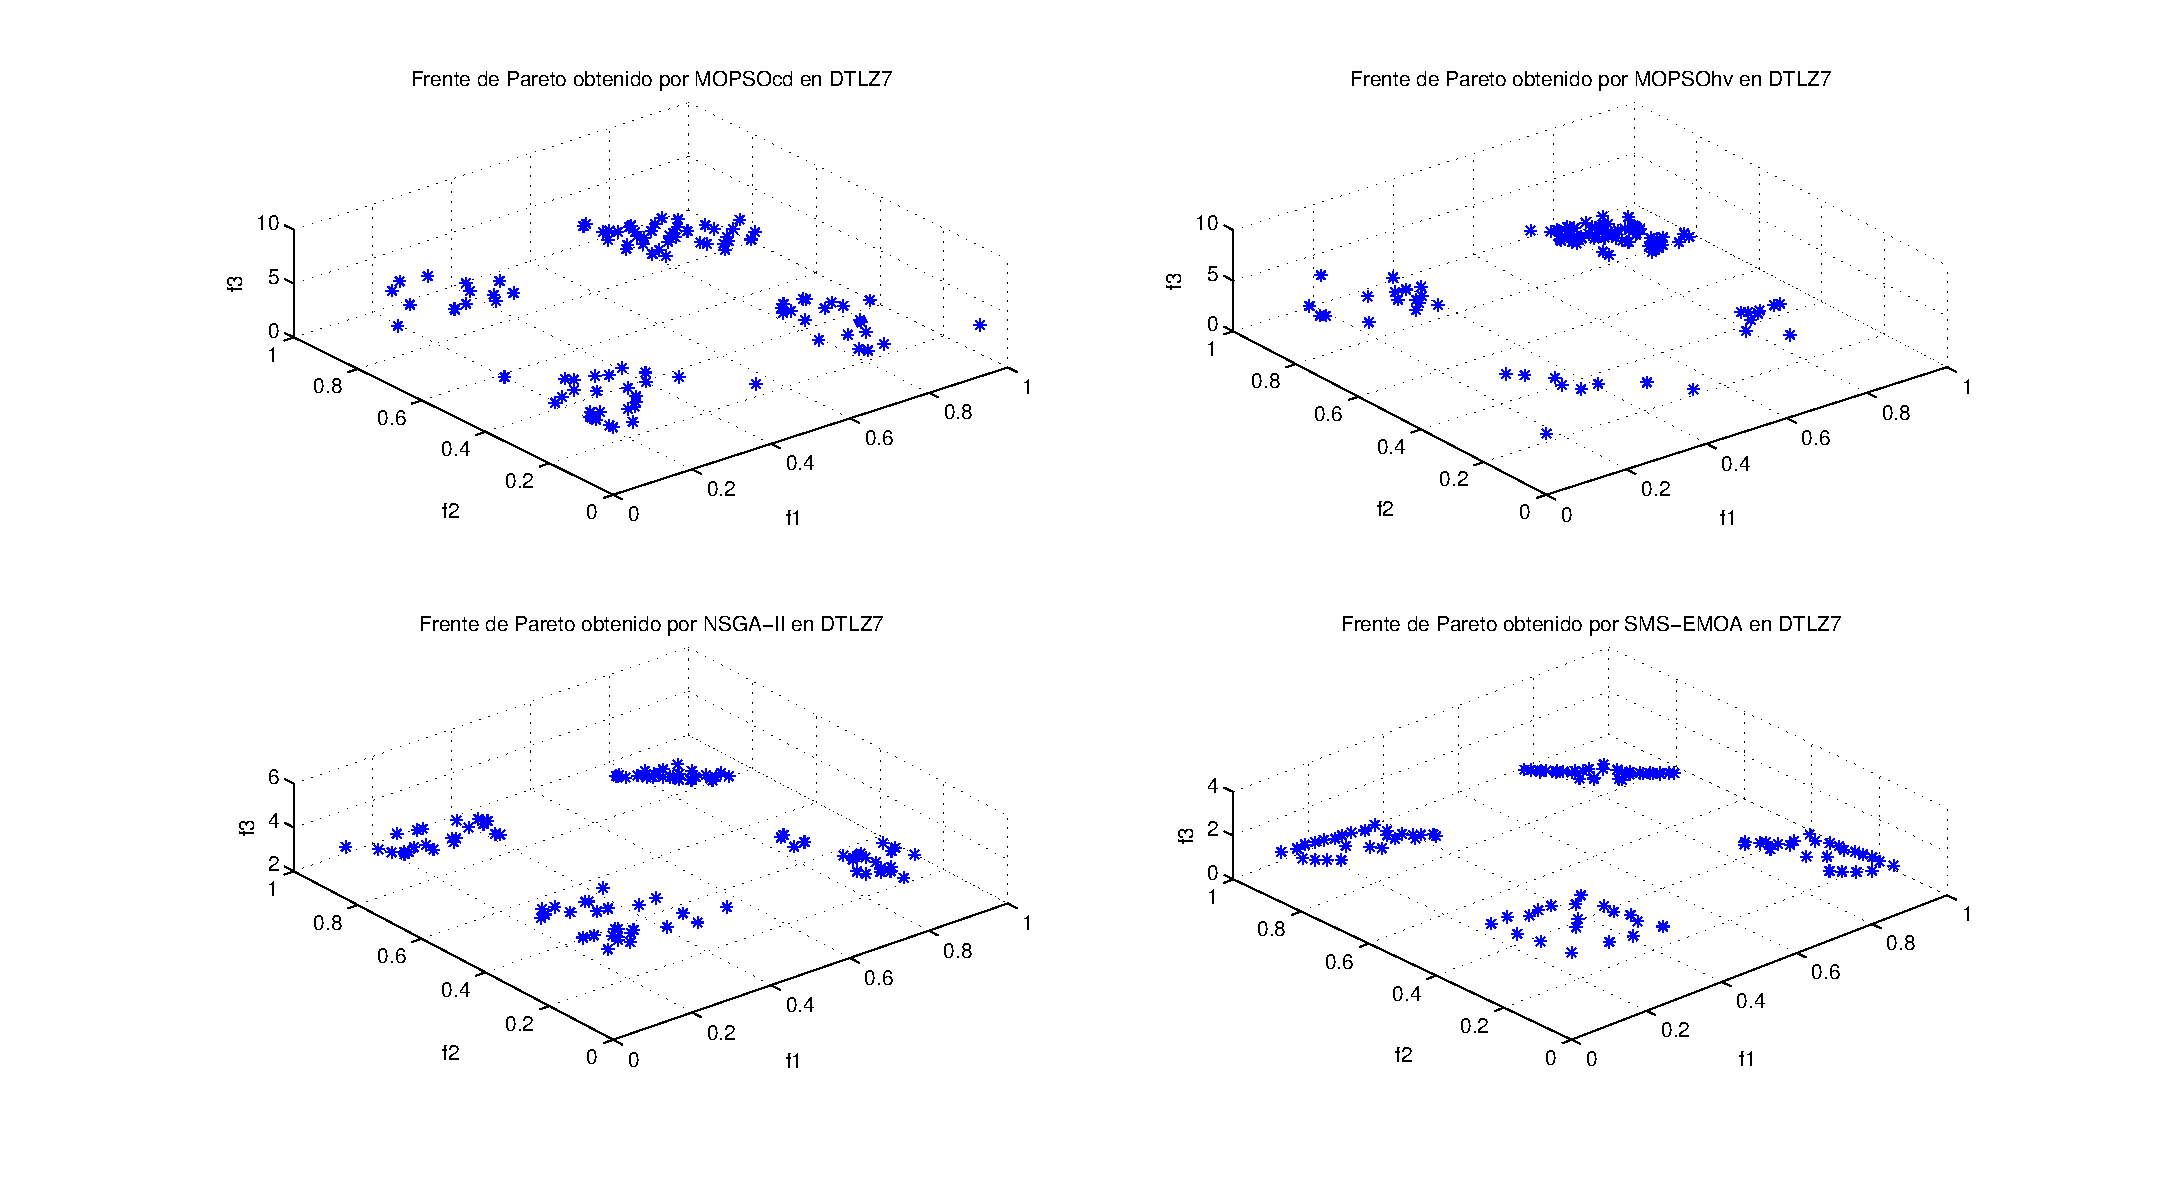
\includegraphics[scale=0.45]{Cap4/rdtlz7r.eps}
      \end{center}
	\caption{Resultados gr\'aficos correspondientes al problema DTLZ7.}
      \label{fig:rDTLZ7}
      \end{figure}
\clearpage


\section{Resultados de escalabilidad}

 Se utiliza el problema DTLZ2 para probar la escalabilidad de nuestro algoritmo de dos a diez objetivos. Las soluciones son comparadas con 
 el NSGA-II, MOPSO-cd y el SMS-EMOA. Se realizaron diez ejecuciones independientes, con 100 individuos y 1200 generaciones usando los 
 par\'ametros de las tablas \ref{tab:parametros1}, \ref{tab:parametros2} y \ref{tab:parametros3}. El punto $\vec{1.1}$ es utlizado como 
 referencia para la m\'etrica del hipervolumen.
 
\begin{longtable}{|l|cc|cc|} 
\hline
    & \multicolumn{4}{|c|}{\textbf{2 Objetivos}} \\ 
	\textbf{Algoritmo} & \textbf{Menor} & \textbf{Mayor} & \textbf{Promedio} & \textbf{Desviaci\'on} \\  \hline \hline
	\textbf{MOPSOhv} & 0.006496 & 0.008450 & \textbf{\textcolor{green}{0.007529}} & \textbf{\textcolor{red}{0.000509}} \\ 
	\textbf{MOPSOcd} & 0.006508 & 0.007755 & \textbf{0.007165} & \textbf{\textcolor{blue}{0.000350}} \\ 
	\textbf{NSGA-II} & 0.006558 & 0.008114 & \textbf{\textcolor{blue}{0.007298}} & \textbf{\textcolor{green}{0.000441}} \\  
	\textbf{SMS-EMOA}& 0.007164 & 0.008134 & \textbf{\textcolor{red}{0.007687}} & \textbf{0.000324}  \\  
	\hline\hline
    & \multicolumn{4}{|c|}{\textbf{3  Objetivos}} \\ 
	\hline\hline
	\textbf{MOPSOhv} & 0.040552 & 0.075311 & \textbf{\textcolor{red}{0.060766}} & \textbf{\textcolor{red}{0.010465}} \\ 
	\textbf{MOPSOcd} & 0.046830 & 0.059367 & \textbf{\textcolor{blue}{0.052755}} & \textbf{\textcolor{blue}{0.003508}} \\ 
	\textbf{NSGA-II} & 0.047551 & 0.062545 & \textbf{\textcolor{green}{0.055653}} & \textbf{\textcolor{green}{0.004653}} \\  
	\textbf{SMS-EMOA}& 0.040739 & 0.045160 & \textbf{0.042945} &\textbf{0.001627} \\
	\hline\hline
    & \multicolumn{4}{|c|}{\textbf{4 Objetivos}} \\ 
	\hline\hline
	\textbf{MOPSOhv} & 0.060814 & 0.103256 & \textbf{\textcolor{blue}{0.076769}} & \textbf{\textcolor{green}{0.013224}} \\ 
	\textbf{MOPSOcd} & 0.255004 & 0.351009 & \textbf{\textcolor{red}{0.307083}} & \textbf{\textcolor{red}{0.029160}} \\ 
	\textbf{NSGA-II} & 0.099124 & 0.121004 & \textbf{\textcolor{green}{0.110590}} & \textbf{\textcolor{blue}{0.007367}} \\  
	\textbf{SMS-EMOA}& 0.060019 & 0.063409 & \textbf{0.061934} & \textbf{0.001271} \\ 
	\hline\hline
 & \multicolumn{4}{|c|}{\textbf{5 Objetivos}} \\ 
	\hline\hline
	\textbf{MOPSOhv} & 0.062663 & 0.115829 & \textbf{0.096073} & \textbf{\textcolor{blue}{0.016611}}    \\ 
	\textbf{MOPSOcd} & 0.357735 & 0.509170 & \textbf{\textcolor{green}{0.439317}} & \textbf{\textcolor{green}{0.048635}} \\ 
	\textbf{NSGA-II} & 0.176407 & 0.213365 & \textbf{\textcolor{blue}{0.194858}} & \textbf{0.012554}  \\  
	\textbf{SMS-EMOA} & --- & --- & \textbf{\textcolor{red}{---}} & \textbf{\textcolor{red}{---}} \\
	\hline\hline
& \multicolumn{4}{|c|}{\textbf{6 Objetivos}} \\ 
	\hline\hline
	\textbf{MOPSOhv} & 0.069909 & 0.146411 & \textbf{0.115437} & \textbf{0.022606}    \\ 
	\textbf{MOPSOcd} & 0.472034 & 0.601704 & \textbf{\textcolor{green}{0.536438}} & \textbf{\textcolor{green}{0.044512}} \\ 
	\textbf{NSGA-II} & 0.326463 & 0.462761 & \textbf{\textcolor{blue}{0.393104}} & \textbf{\textcolor{blue}{0.040260}} \\  
	\textbf{SMS-EMOA} & --- & --- & \textbf{\textcolor{red}{---}} & \textbf{\textcolor{red}{---}} \\
	\hline\hline
 & \multicolumn{4}{|c|}{\textbf{7 Objetivos}} \\ 
	\hline\hline
	\textbf{MOPSOhv} & 0.104604 & 0.198331 & \textbf{0.134378} & \textbf{0.027768}   \\ 
	\textbf{MOPSOcd} & 0.567486 & 0.800344 & \textbf{\textcolor{green}{0.666199}} & \textbf{\textcolor{green}{0.064909}}  \\ 
	\textbf{NSGA-II} & 0.555849 & 0.750226 & \textbf{\textcolor{blue}{0.626970 }}& \textbf{\textcolor{blue}{0.053539}} \\  
	\textbf{SMS-EMOA} & --- & --- & \textbf{\textcolor{red}{---}} &\textbf{\textcolor{red}{ --- }}\\
	\hline\hline
 & \multicolumn{4}{|c|}{\textbf{8 Objetivos}} \\ 
	\hline\hline
	\textbf{MOPSOhv} & 0.091730 & 0.173281 & \textbf{0.122761} & \textbf{0.025681}   \\ 
	\textbf{MOPSOcd} & 0.656487 & 0.898391 & \textbf{\textcolor{blue}{0.768978}} & \textbf{\textcolor{green}{0.083783}} \\ 
	\textbf{NSGA-II} & 0.707636 & 0.843402 & \textbf{\textcolor{green}{0.773139}} & \textbf{\textcolor{blue}{0.048302}} \\ 
	\textbf{SMS-EMOA} & --- & --- &\textbf{\textcolor{red}{ ---}} & \textbf{\textcolor{red}{--- }}\\
	\hline\hline
 & \multicolumn{4}{|c|}{\textbf{9 Objetivos}} \\ 
	\hline\hline
	\textbf{MOPSOhv} &0.069848 & 0.150881 & \textbf{0.109239} & \textbf{0.026673}   \\ 
	\textbf{MOPSOcd} & 0.656487 & 0.898391 & \textbf{\textcolor{blue}{0.768978}} & \textbf{\textcolor{green}{0.083783}} \\ 
	\textbf{NSGA-II} &0.883374 & 0.977749 & \textbf{\textcolor{green}{0.913665}} & \textbf{\textcolor{blue}{0.025785}} \\ 
	\textbf{SMS-EMOA} & --- & --- & \textbf{\textcolor{red}{---}} &\textbf{\textcolor{red}{ ---}} \\
	\hline\hline
 & \multicolumn{4}{|c|}{\textbf{10 Objetivos}} \\ 
	\hline\hline
	\textbf{MOPSOhv} &0.090387 & 0.180091 & \textbf{0.129630} & \textbf{0.028221}    \\ 
	\textbf{MOPSOcd} &0.682277 & 0.953287 & \textbf{\textcolor{blue}{0.826685}} & \textbf{\textcolor{green}{0.093907}}  \\ 
	\textbf{NSGA-II} &0.936894 & 1.132359 & \textbf{\textcolor{green}{1.032422}} & \textbf{\textcolor{blue}{0.071610}}\\  
	\textbf{SMS-EMOA} & --- & --- & \textbf{\textcolor{red}{---}} &\textbf{\textcolor{red}{ ---}} \\
	\hline\hline
\caption{Resultados de la m\'etrica de espaciado para DTLZ2 de 2 a 10 objetivos.}
  \label{tab:dtlz2_es}
\end{longtable}
 
 La tabla \ref{tab:dtlz2_es} muestra como la distribuci\'on de las soluciones mejoran para nuestra propuesta al aumentar el n\'umero 
 de objetivos del problema DTLZ2. Mientras que en el NSGA-II y MOPSOcd el valor de la m\'etrica de espaciado crece al aumentar el n\'umero
 de objetivos nuestra propuesta se mantiene constante.
 
\begin{longtable}{|l|cc|cc|} 
\hline
    & \multicolumn{4}{|c|}{\textbf{2 Objetivos}} \\ 
	\textbf{Algoritmo} & \textbf{Menor} & \textbf{Mayor} & \textbf{Promedio} & \textbf{Desviaci\'on} \\  \hline \hline
	\textbf{MOPSOhv} & 0.420910 & 0.420993 & \textbf{\textcolor{blue}{0.420962}} &\textbf{\textcolor{blue}{ 0.000031}}\\ 
	\textbf{MOPSOcd} & 0.420317 & 0.420437 & \textbf{\textcolor{green}{0.420372}} &\textbf{\textcolor{green}{ 0.000037}}\\ 
	\textbf{NSGA-II} & 0.418849 & 0.419966 & \textbf{\textcolor{red}{0.419588}} &\textbf{\textcolor{red}{ 0.000323}}\\  
	\textbf{SMS-EMOA}& 0.421020 & 0.421027 & \textbf{0.421023} & \textbf{0.000003}\\  
	\hline\hline
    & \multicolumn{4}{|c|}{\textbf{3  Objetivos}} \\ 
	\hline\hline
	\textbf{MOPSOhv} & 0.597900 & 0.697158 & \textbf{\textcolor{red}{0.644946}} & \textbf{\textcolor{red}{0.030303}}\\ 
	\textbf{MOPSOcd} & 0.622449 & 0.698677 & \textbf{\textcolor{green}{0.667862}} & \textbf{\textcolor{green}{0.024190}}\\ 
	\textbf{NSGA-II} & 0.676373 & 0.708493 & \textbf{\textcolor{blue}{0.697689}} & \textbf{\textcolor{blue}{0.009213}}\\  
	\textbf{SMS-EMOA}& 0.757991 & 0.758168 & \textbf{0.758071} & \textbf{0.000056}\\
	\hline\hline
    & \multicolumn{4}{|c|}{\textbf{4 Objetivos}} \\ 
	\hline\hline
	\textbf{MOPSOhv} &0.570237 & 0.735955 & \textbf{\textcolor{green}{0.649871}} & \textbf{\textcolor{green}{0.046065}} \\ 
	\textbf{MOPSOcd} &0.000000 & 0.000000 & \textbf{\textcolor{red}{0.000000}} & \textbf{\textcolor{red}{0.000000}} \\ 
	\textbf{NSGA-II} &0.805413 & 0.876853 & \textbf{\textcolor{blue}{0.834518}} & \textbf{\textcolor{blue}{0.019843}} \\  
	\textbf{SMS-EMOA}&1.044708 & 1.044792 & \textbf{1.044734} & 0.000030 \\ 
	\hline\hline
 & \multicolumn{4}{|c|}{\textbf{5 Objetivos}} \\ 
	\hline\hline
	\textbf{MOPSOhv} &0.526935 & 0.821024 & \textbf{\textcolor{blue}{0.686608}} & \textbf{\textcolor{blue}{0.091850}} \\ 
	\textbf{MOPSOcd} &0.000000 & 0.000000 & \textbf{\textcolor{red}{0.000000}} & \textbf{\textcolor{red}{0.000000}} \\ 
	\textbf{NSGA-II} &0.624795 & 0.874966 & \textbf{0.806271} & \textbf{0.075088}\\  
	\textbf{SMS-EMOA}& --- & --- & \textbf{\textcolor{green}{---}} & \textbf{\textcolor{green}{---}} \\
	\hline\hline
& \multicolumn{4}{|c|}{\textbf{6 Objetivos}} \\ 
	\hline\hline
	\textbf{MOPSOhv} &0.588840 & 0.897113 & \textbf{0.768027} & \textbf{0.106912} \\ 
	\textbf{MOPSOcd} &0.000000 & 0.000000 & \textbf{\textcolor{red}{0.000000}} & \textbf{\textcolor{red}{0.000000}} \\ 
	\textbf{NSGA-II} &0.016168 & 0.385332 & \textbf{\textcolor{blue}{0.195606}} & \textbf{\textcolor{blue}{0.133364}} \\  
	\textbf{SMS-EMOA}& --- & --- & \textbf{\textcolor{green}{---}} &\textbf{\textcolor{green}{ --- }}\\
	\hline\hline
 & \multicolumn{4}{|c|}{\textbf{7 Objetivos}} \\ 
	\hline\hline
	\textbf{MOPSOhv} &0.779870 & 0.986701 & \textbf{0.897171} & \textbf{0.059289} \\ 
	\textbf{MOPSOcd} &0.000000 & 0.000000 & \textbf{\textcolor{red}{0.000000}} & \textbf{\textcolor{red}{0.000000}} \\ 
	\textbf{NSGA-II} &0.000960 & 0.336963 & \textbf{\textcolor{blue}{0.146724}} & \textbf{\textcolor{blue}{0.119704}} \\  
	\textbf{SMS-EMOA} & --- & --- & \textbf{\textcolor{green}{---}} & \textbf{\textcolor{green}{---}} \\
	\hline\hline
 & \multicolumn{4}{|c|}{\textbf{8 Objetivos}} \\ 
	\hline\hline
	\textbf{MOPSOhv} &0.711453 & 1.069716 & \textbf{0.923948} & \textbf{\textcolor{blue}{0.098939}} \\ 
	\textbf{MOPSOcd} &0.000000 & 0.000000 & \textbf{\textcolor{red}{0.000000}} & \textbf{\textcolor{red}{0.000000}} \\ 
	\textbf{NSGA-II} &0.071442 & 0.358558 & \textbf{\textcolor{blue}{0.185958}} & \textbf{0.088435}\\ 
	\textbf{SMS-EMOA} & --- & --- & \textbf{\textcolor{green}{---}} & \textbf{\textcolor{green}{---}} \\
	\hline\hline
 & \multicolumn{4}{|c|}{\textbf{9 Objetivos}} \\ 
	\hline\hline
	\textbf{MOPSOhv} &0.767567 & 1.063881 & \textbf{0.894945} & \textbf{\textcolor{blue}{0.098291}} \\ 
	\textbf{MOPSOcd} &0.000000 & 0.000000 & \textbf{\textcolor{red}{0.000000}} & \textbf{\textcolor{red}{0.000000}} \\ 
	\textbf{NSGA-II} &0.039463 & 0.397496 & \textbf{\textcolor{blue}{0.212041}} & \textbf{0.124973} \\ 
	\textbf{SMS-EMOA} & --- & --- & \textbf{\textcolor{green}{---}} & \textbf{\textcolor{green}{---}} \\
	\hline\hline
 & \multicolumn{4}{|c|}{\textbf{10 Objetivos}} \\ 
	\hline\hline
	\textbf{MOPSOhv} &0.946736 & 1.228404 & \textbf{1.080952} & \textbf{0.085351}   \\ 
	\textbf{MOPSOcd} &0.000000 & 0.000000 & \textbf{\textcolor{red}{0.000000}} & \textbf{\textcolor{red}{0.000000}} \\ 
	\textbf{NSGA-II} &0.015169 & 0.440330 & \textbf{\textcolor{blue}{0.224003}} & \textbf{\textcolor{blue}{0.127577}} \\  
	\textbf{SMS-EMOA} & --- & --- & \textbf{\textcolor{green}{---}} & \textbf{\textcolor{green}{---}} \\
	\hline\hline
\caption{Resultados de la m\'etrica de hipervolumen para DTLZ2 con 2 a 10 objetivos.}
  \label{tab:dtlz2_hv}
\end{longtable}

La tabla \ref{tab:dtlz2_hv} muestra los resultados obtenidos para la m\'etrica del hipervolumen para el problema 
DTLZ2 con 2 a 10 objetivos. El NSGA-II muestra un deterioro en la 
calidad de las soluciones cuando aumenta el n\'umero de objetivos del problema con un costo 
computacional bajo. El SMS-EMOA muestra tener buenos resultados, pero es muy costoso, 
computacionalmente hablando. 
MOPSOcd muestra que su desempe\~no no es escalable ya que se degrada r\'apidamente al aumentar el n\'umero de 
funciones objetivo. 

Conforme a estos resultados se puede crear una
jerarqu\'ia en orden descendente en t\'erminos del valor del hipervolumen del conjunto de soluciones pr\'oximas al frente de Pareto real:

\begin{enumerate}
  \item MOPSOhv
  \item NSGA-II
  \item SMS-EMOA
  \item MOPSOcd
\end{enumerate}

Nuestra propuesta muestra tener buenos resultados en la
calidad de las soluciones cuando aumentan el n\'umero de objetivos del problema al mantenerse constante en la m\'etrica del 
hipervolumen y manteniendo un costo computacional razonable, lo que hace a nuestro algoritmo competitivo respecto a los dem\'as como se muestra en 
la figura \ref{fig:tescala}.

  \begin{figure}
      \begin{center}
	  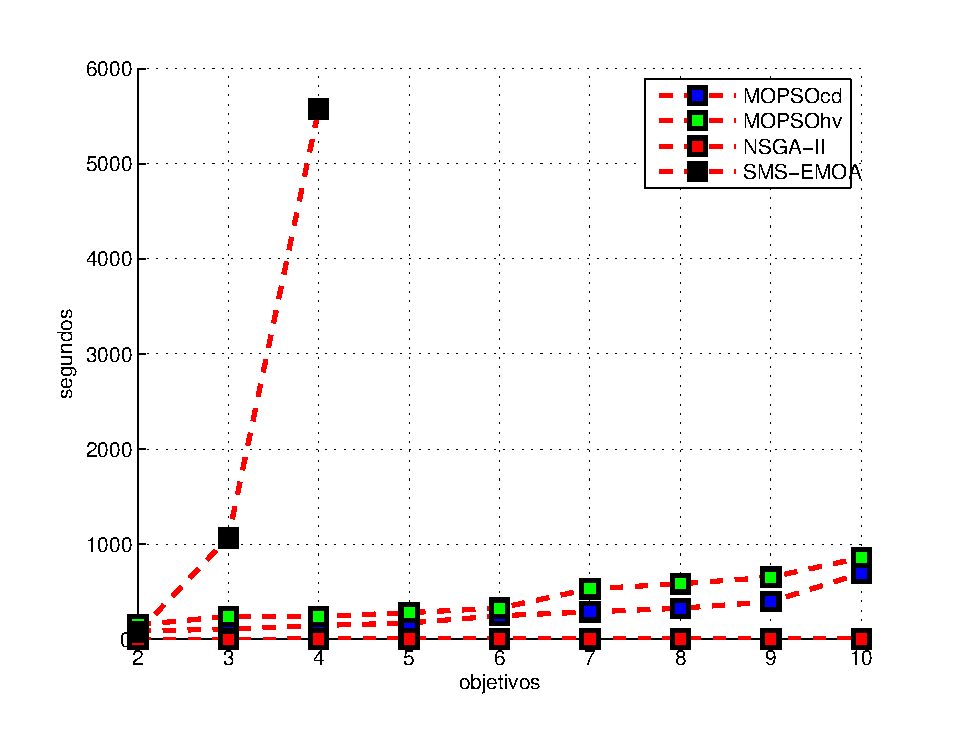
\includegraphics[scale=1]{Cap4/tiempoEscala.eps}
      \end{center}
	\caption[Tiempos en escalamiento para el problema DTLZ2.]{Resultados de tiempo en segundos aumentando el n\'umero 
	de objetivos del problema DTLZ2.}
      \label{fig:tescala}
  \end{figure}

 
\begin{chapter}{Conclusiones y trabajo futuro}
  
  \section{Resumen}
  
  El objetivo principal de este trabajo de tesis fue proponer un nuevo algoritmo multi-objetivo basado los c\'umulos de 
  part\'iculas la cual mostrara ser competitiva con respecto a algoritmos evolutivos multiobjetivo (AEMOs) representativos del estado 
  del arte.

  Para llevar a cabo este objetivo se realiz\'o un estudio de las metaheur\'isticas multi-objetivo basadas en 
  c\'umulos de part\'iculas que existen actualmente. Posteriormente, se realiz\'o un estudio del denominado hipervolumen 
  para poder incorporarlo en el mecanismo de selecci\'on de nuestra metaheur\'istica. A este respecto, se identificaron
  varias formas de utilizar el hipervolumen como mecanismo de selecci\'on, sobresaliendo
  el uso del algoritmo HypE que usa un m\'etodo para aproximar las contribuciones al hipervolumen. 
  Como producto de este an\'alisis se propuso un algoritmo de c\'umulos de part\'iculas multi-objetivo que aprovecha las contribuciones al 
  hipervolumen para seleccionar la mejor gu\'ia global a fin de generar soluciones potenciales no dominadas.

  El algoritmo propuesto fue comparado con respecto a NSGA-II, SMS-EMOA y MOPSOcd. La evaluaci\'on se realiz\'o utilizando un conjunto 
  de problemas multi-objetivo que re\'unen diferentes 
  caracter\'isticas que causan dificultades a un algoritmo evolutivo multi-objetivo.
  
  \section{Conclusiones}
  
  A partir de los experimentos realizados se desprenden las siguientes conclusiones:

  \begin{itemize}
  \item Una de las principales dificultades en extender el algoritmo del PSO a una versi\'on multi-objetivo, es encontrar la mejor 
  forma de seleccionar al l\'ider de cada part\'icula en el c\'umulo. Esta dificultad radica en que no hay una noci\'on clara sobre 
  c\'omo definir qui\'en es el mejor alcanzado hasta el momento (\textbf{\textit{pBest}}) y el mejor 
  alcanzado por toda la poblaci\'on (\textbf{\textit{gBest}}). En los problemas de optimizaci\'on multi-objetivo, 
  todas las soluciones no dominadas son igualmente buenas, por lo que cualquiera de ellas puede adoptarse como l\'ider. Por tanto, el 
  uso del hipervolumen nos permiti\'o seleccionar al mejor l\'ider alcanzado de un conjunto de soluciones no dominadas. La selecci\'on
  se realiza conforme a su contribuci\'on al hipervolumen, es decir, aquella part\'icula que contribuye m\'as al valor del hipervolumen
  es seleccionada como l\'ider.
  
  \item El uso del hipervolumen para seleccionar al l\'ider en nuestro algoritmo muestra una mejora con respecto al algoritmo MOPSOcd. 
  
  \item La forma de seleccionar al conjunto de part\'iculas que influyen en el entorno social  del algoritmo ($pBest$) mejora 
  considerablemente la b\'usqueda de nuevas soluciones no dominadas. Es mejor utilizar el archivo o la poblaci\'on
  secundaria, en lugar de la poblacion primaria, para actualizar el $pBest$ del algoritmo propuesto.
  
  \item La contribuci\'on al hipervolumen es un valor que se basa en la m\'etrica del hipervolumen. Por lo que, resulta ser muy costoso 
  computacionalmente hablando. Sin embargo, el uso de algoritmos que hacen uso de metodos 
  de muestreo para calcular la contribuci\'on al hipervolumen resultan ser m\'as eficientes. El uso de HypE 
  es un algoritmo que utiliza el m\'etodo de Monte Carlo y muestra ser m\'as eficiente al calcular las contribuciones al hipervolumen.
  
  \item El uso del algoritmo de HypE para calcular las contribuciones al hipervolumen permite aumentar el n\'umero de generaciones 
  del algoritmo y el n\'umero de objetivos del problema.
  
  \item Debido a que se utiliza una aproximaci\'on de la contribuci\'on al hipervolumen, se decidi\'o utilizar un operador de 
  turbulencia para evitar quedar atrapado en frentes de Pareto locales.
  
  \item Los resultados obtenidos en promedio para los primeros tres problemas ZDT son similares. Para el problema ZDT4 es mejor que 
  los resultados obtenidos por el SMS-EMOA y marginalmente peores que los del NSGA-II. As\'i mismo, nuestros resultados 
  son mejores que los de MOPSOcd. Para el problema ZDT6 los resultados son ligeramente mejores que los de SMS-EMOA 
  y ligeramente peores que los de NSGA-II, siendo mucho mejores que los del MOPSOcd.
  
  \item Los resultados obtenidos por nuestra propuesta para los problemas DTLZ1, DTLZ3 y DTLZ6 son mejores que los del MOPSOcd.
  Sin embargo, nuestro algoritmo no pudo obtener buenas aproximaciones al frente de Pareto real, y nuestros resultados fueron dominados
  por los de SMS-EMOA y NSGA-II. Los resultados para los dem\'as problemas (DTLZ2, DTLZ4, DTLZ5 y DTLZ7) muestran que en la mayoria 
  de los casos, nuestra propuesta obtiene soluciones que dominan a las de los algoritmos NSGA-II, SMS-EMOA y MOPSOcd.
  
  \item Los resultados obtenidos de nuestra propuesta muestran que en la mayoria de los problemas (2 y 3 objetivos), en promedio ,es competitiva
  con respecto a los algoritmos NSGA-II, SMS-EMOA y MOPSOcd.
  
  \item Nuestro algoritmo mantiene un buen desempe\~no al aumentar el n\'umero de objetivos del problema, manteniendo un costo computacional 
  razonable. Esto hace que nuestro algoritmo sea competitivo con respecto a los algoritmos NSGA-II, al SMS-EMOA y al MOPSOcd.
  \end{itemize}
  
  \section{Trabajo futuro}
  
  Existen diversas formas de poder dise\~nar un algoritmo multi-objetivo con base en la metaheur\'istica de c\'umulos de 
  part\'iculas, pues es posible usar diferentes tipos de topolog\'ias o conexiones para que las part\'iculas interact\'uen o 
  influyan entre ellas a fin de generar buenas aproximaciones hacia el verdadero frente de Pareto.
 
  En particular se podr\'ian realizar las siguientes extensiones a nuestro algoritmo:
  
  \begin{itemize}
  \item Utilizar modelos de configuraci\'on diferentes al modelo completo que se us\'o aqu\'i 
   (modelo cognitivo, modelo social o modelo social exclusivo). 
  \item Utilizar otros apectos avanzados que pueden acelerar la convergencia del algoritmo (factor de constricci\'on, factor de inercia 
  adaptable o control de velocidad).
  
 \item Seleccionar a los gu\'ias locales de otra manera, de tal forma, que afecten la parte cognitiva del algoritmo permitiendo
 generar nuevas soluciones.
 
 \item Seleccionar un mejor estimador de densidad para hacer el reemplazo de los soluciones no dominadas en la poblaci\'on secundaria.
 
 \end{itemize}  
\end{chapter}

\appendix
%\begin{chapter}{Funciones de Prueba}

\section*{ZDT (Zitzler-Deb-Thiele)} 

\textbf{Formulaci\'on de ZDT1:}

\begin{align*}
f_1(x)&=x_1\\
f_2(x,g(x))&=g(x)\cdot\left(1-\sqrt{ \frac{f_1}{g(x)}}\right)\\
g(x)&=1+\frac{9}{n-1}\cdot\sum_{i=2}^nx_i
\end{align*}

donde $n=30$ y $x_i\in[0,1]$ con $i=1,\ldots, n$. El \textit{frente de Pareto real} ($\mathcal{F}_{real}$) se forma con $g(x)=1$ y se muestra
en la figura \ref{fig:ZDT1}. Tiene un \textit{frente de Pareto} convexo.

\begin{figure}[h!]
 \centering
    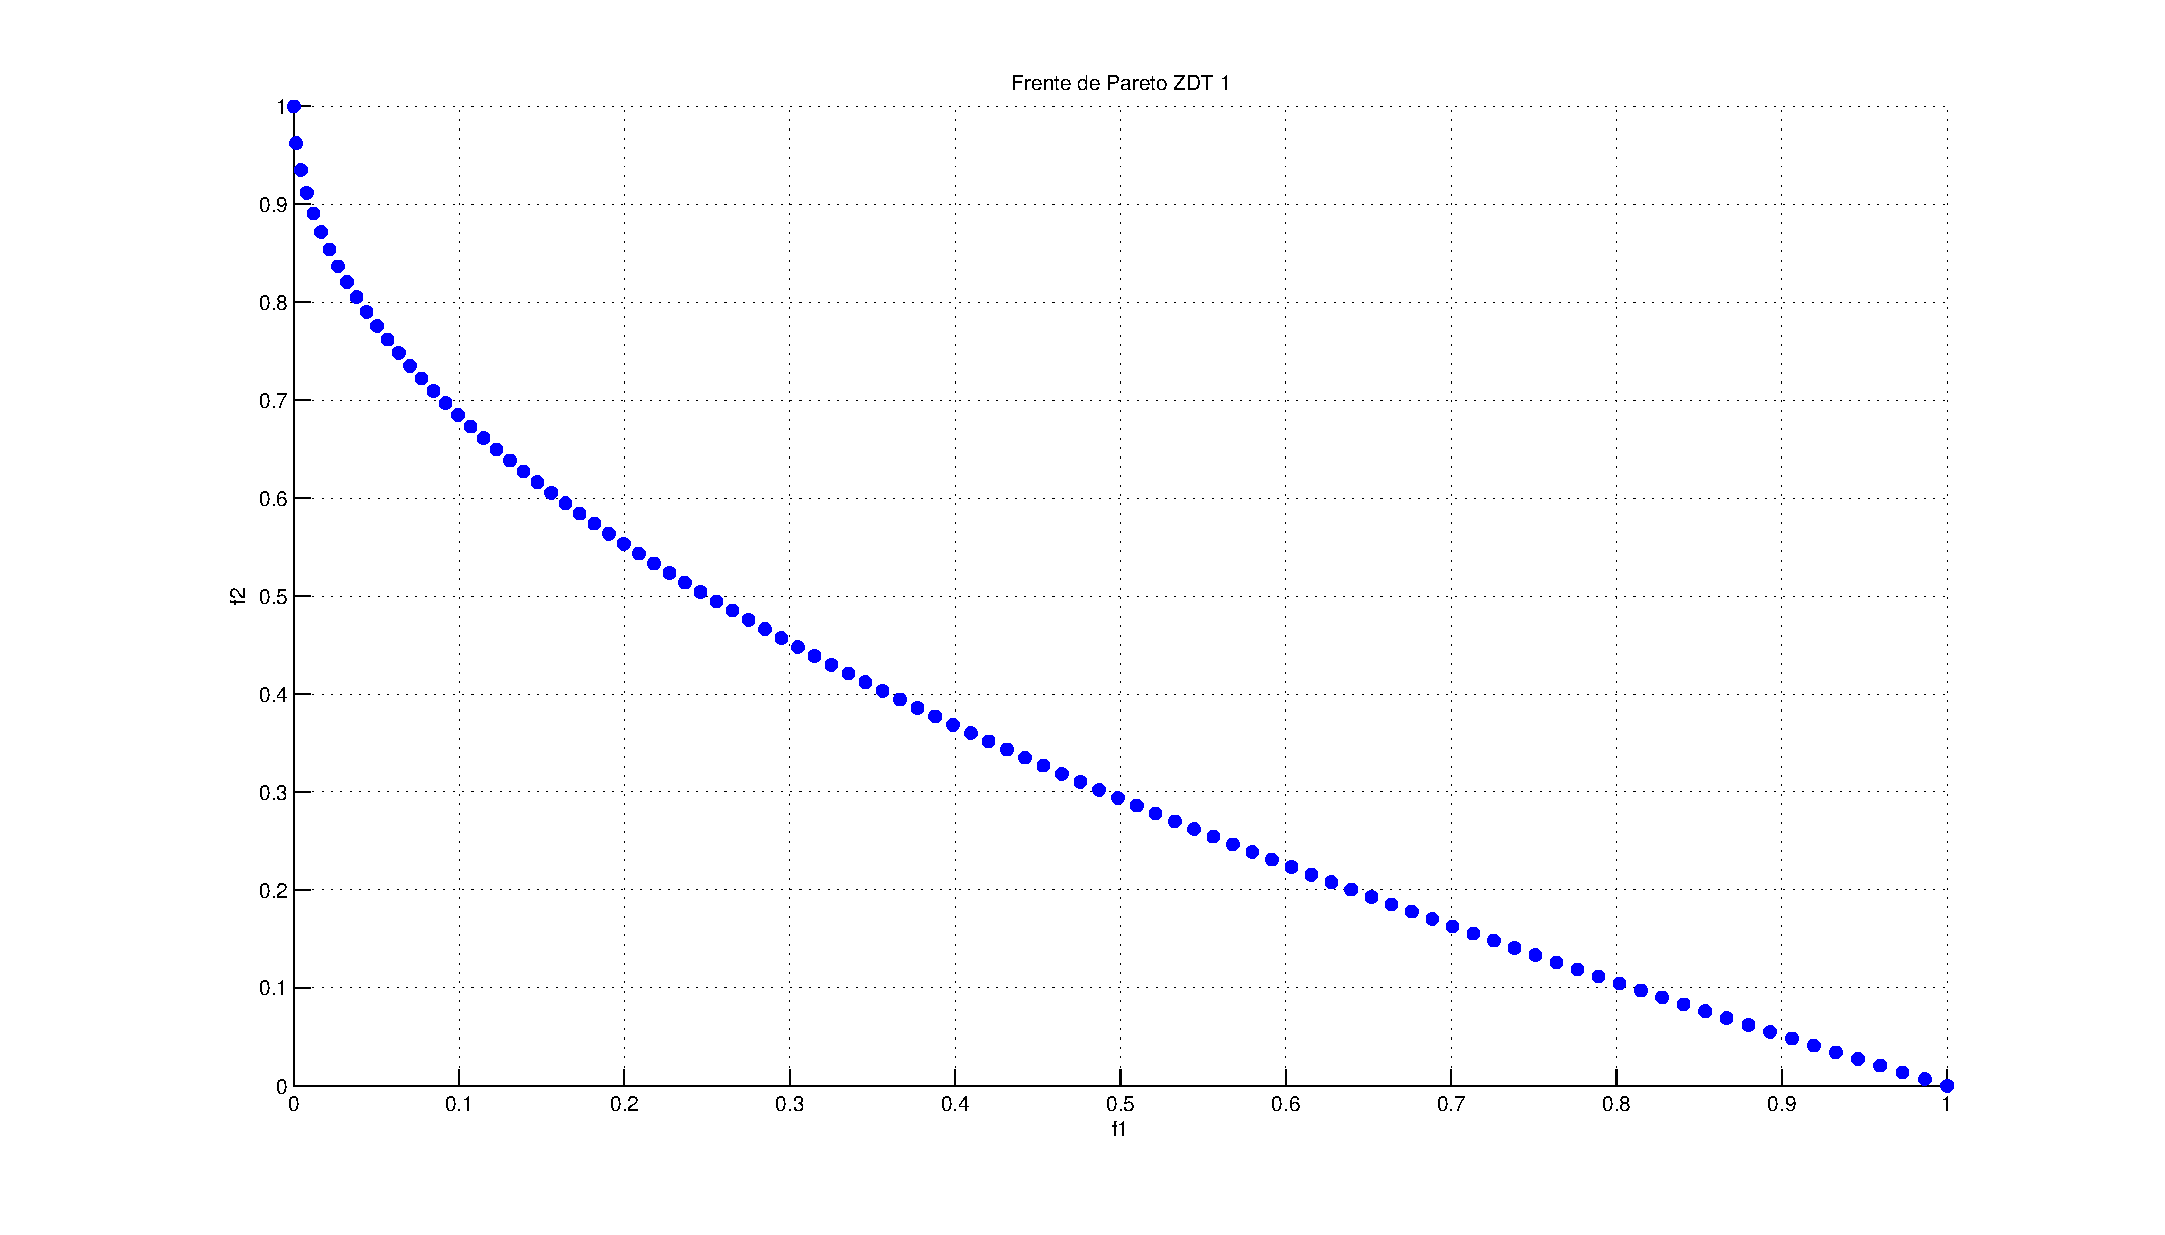
\includegraphics[scale=0.43]{ApendiceA/paretoZDT1.eps}
\caption{Frente de Pareto ZDT1}
\label{fig:ZDT1}
\end{figure} 

\textbf{Formulaci\'on de ZDT2:}

\begin{align*}
f_1(x)&=x_1\\
f_2(x,g(x))&=g(x)\cdot(1- \left( \frac{f_1}{g(x)}\right)^2)\\
g(x)&=1+\frac{9}{n-1}\cdot\sum_{i=2}^nx_i
\end{align*}

donde $n=30$ y $x_i\in[0,1]$ con $i=1,\ldots, n$. El \textit{frente de Pareto real} ($\mathcal{F}_{real}$) se forma con $g(x)=1$ y se muestra 
en la figura \ref{fig:ZDT2}. Tiene un \textit{frente de Pareto} c\'oncavo.

\begin{figure}[h!]
 \centering
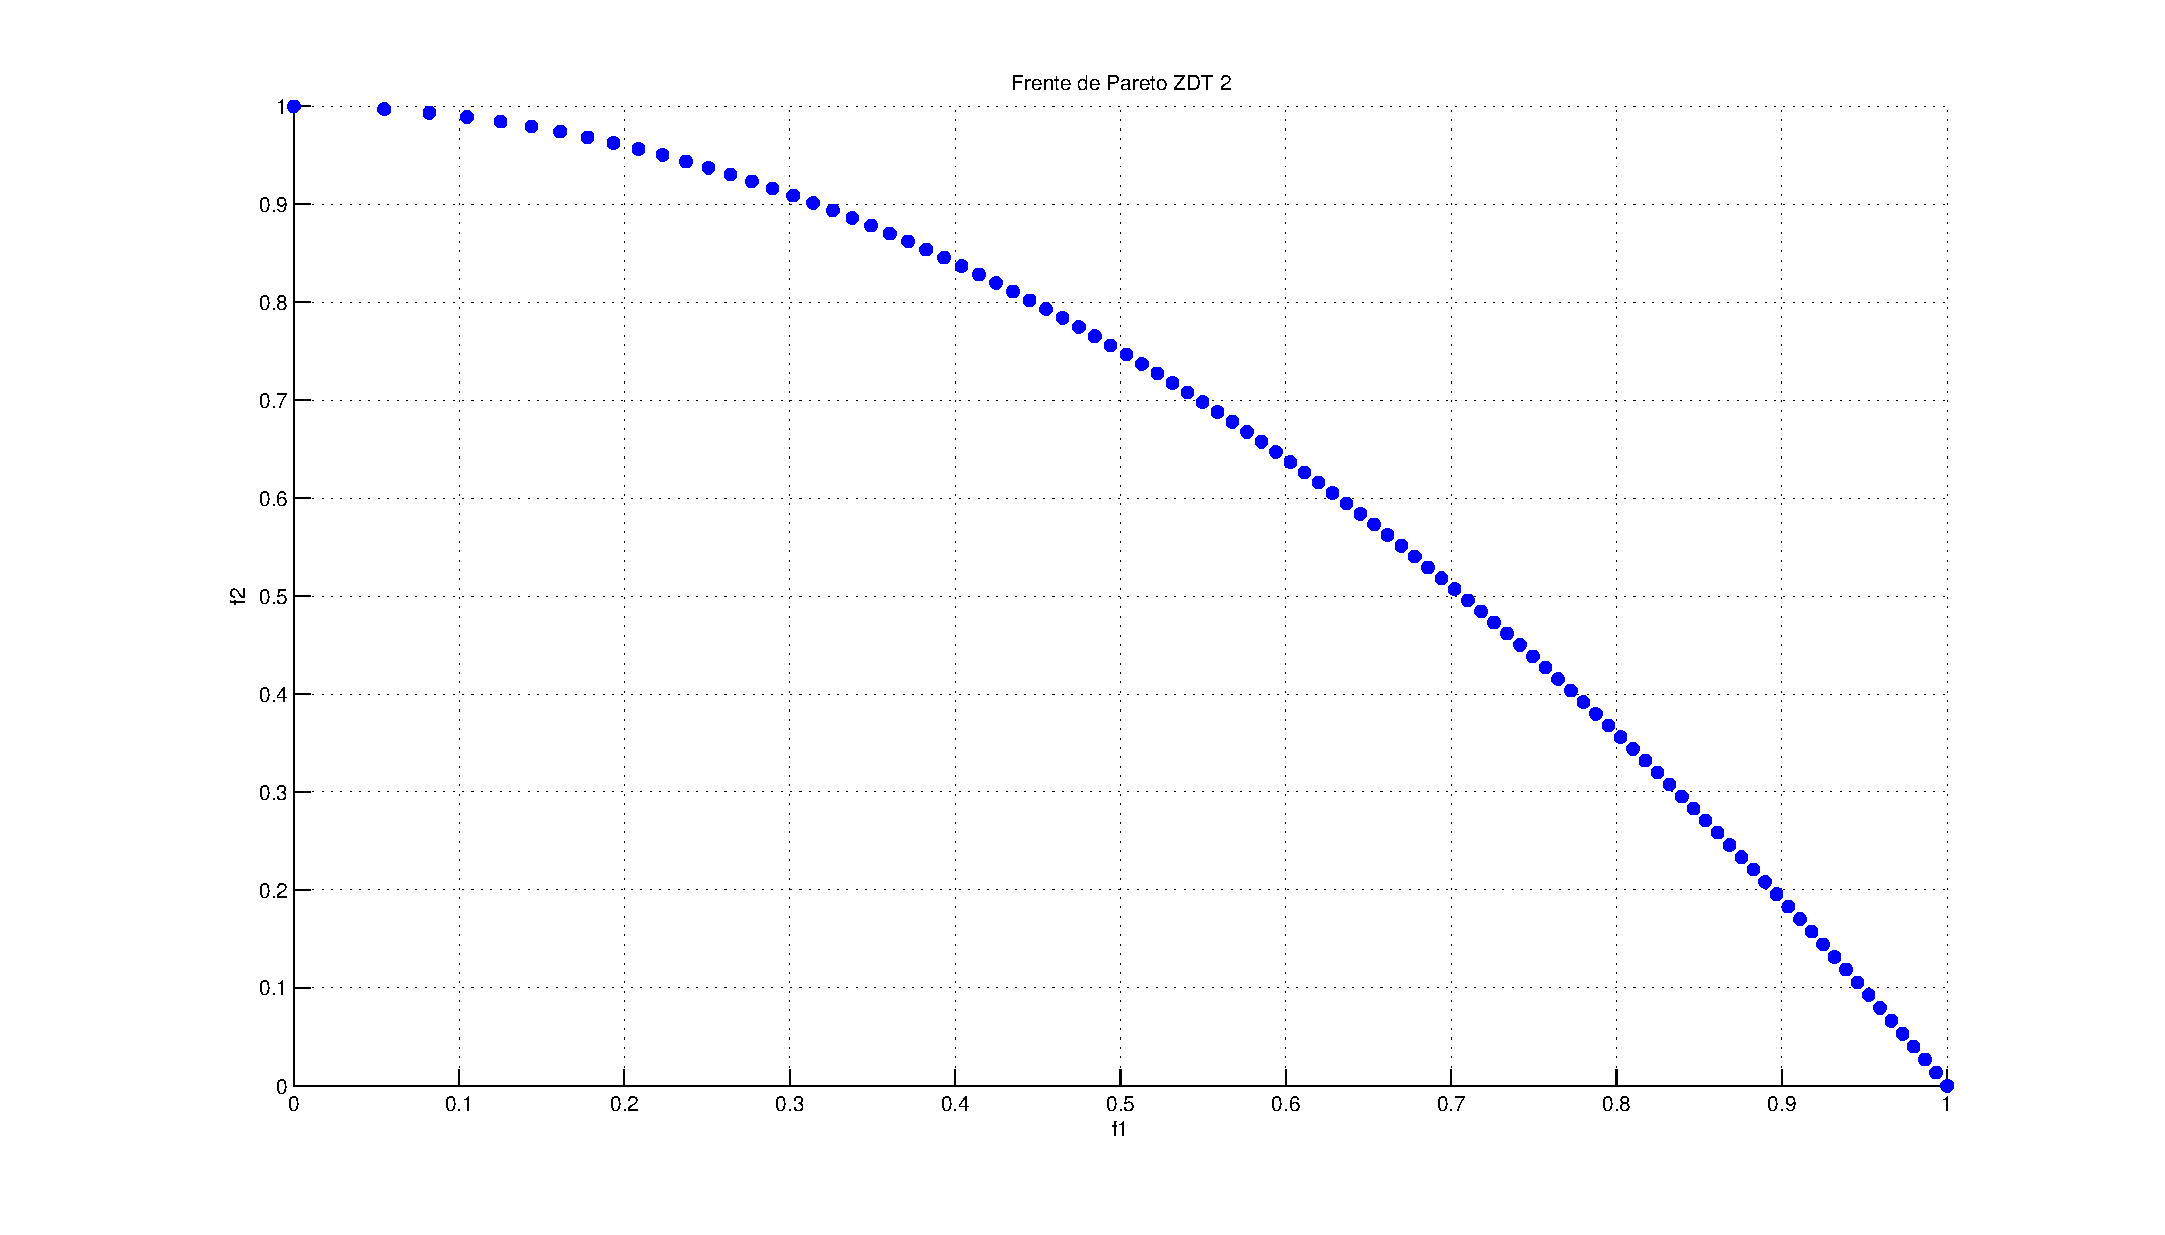
\includegraphics[scale=0.45]{ApendiceA/paretoZDT2.eps}
\caption{Frente de Pareto ZDT2}
\label{fig:ZDT2}
\end{figure} 

\textbf{Forumulaci\'on de ZDT3:}

\begin{align*}
f_1(x)&=x_1,\\
f_2(x,g)&=g(x)\cdot\left(1-\sqrt{\frac{f_1(x)}{g(x)}}-\frac{f_1(x)}{g(x)}\sin(10\cdot\pi\cdot f_1(x))\right)\\
g(x)&=1+\frac{9}{n-1}\cdot\sum_{i=2}^nx_i
\end{align*}

donde $n=30$ y $x_i\in[0,1]$ con $i=1, \ldots, n$. El \textit{frente de Pareto real} ($\mathcal{F}_{real}$) se forma con $g(x)=1$ y se muestra 
en la figura \ref{fig:ZDT3}. Tiene un {\it frente de Pareto} discontinuo y convexo.

\begin{figure}[h!]
 \centering
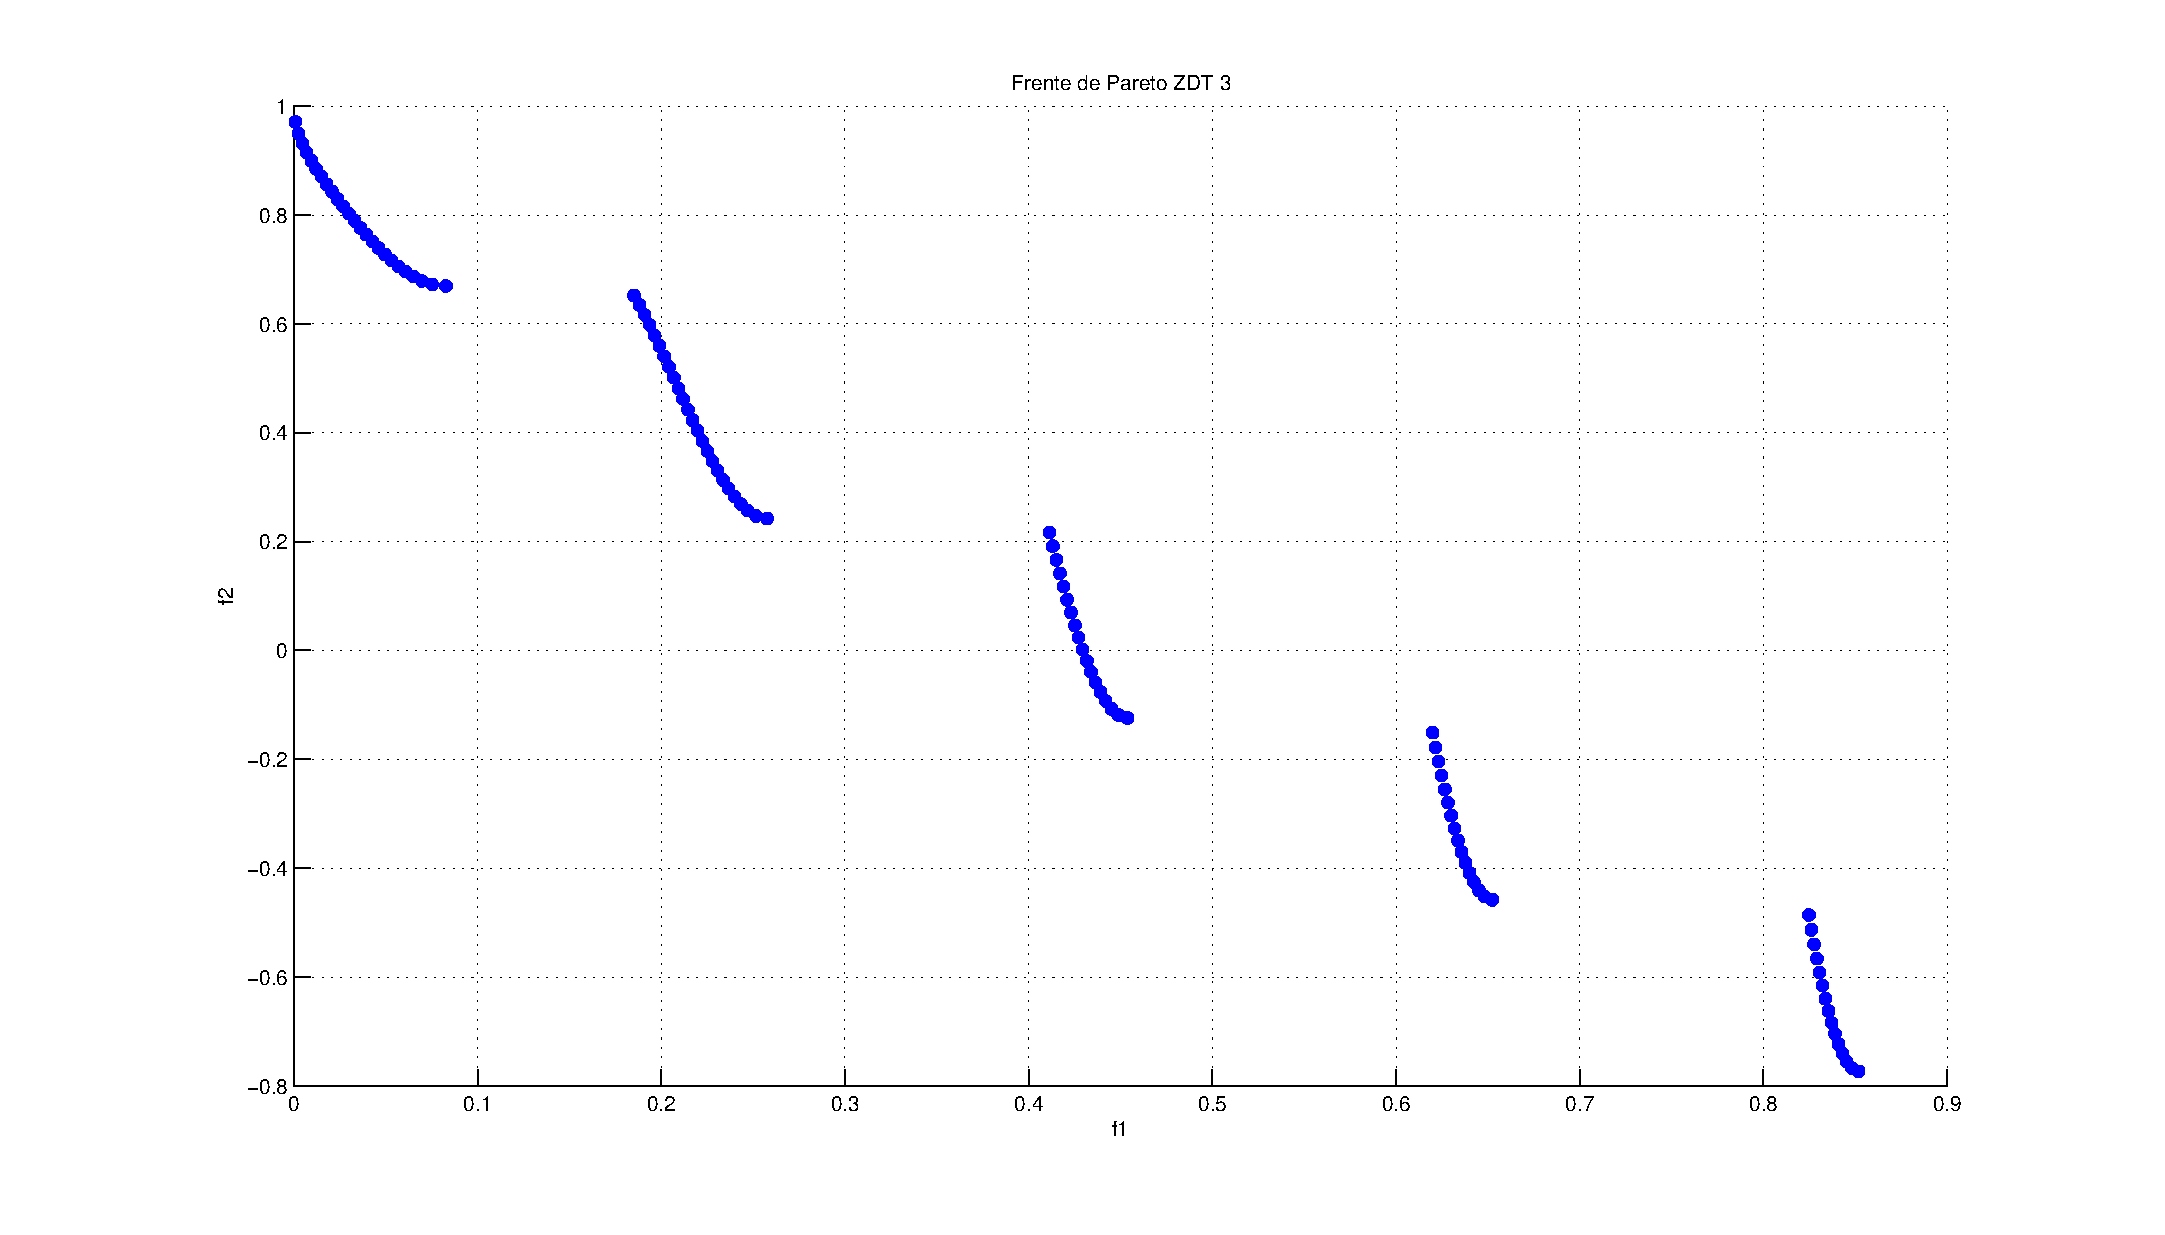
\includegraphics[scale=0.45]{ApendiceA/paretoZDT3.eps}
\caption{Frente de Pareto ZDT3}
\label{fig:ZDT3}
\end{figure} 

\textbf{Forumulaci\'on de ZDT4:}

\begin{align*}
f_1(x)&=x_1,\\
f_2(x,g(x))&=g(x)\cdot \left(1-\sqrt{ \frac{f_1(x)}{g(x)}}\right),\\
g(x)&=1+10\cdot(n-1)+ \sum_{i=2}^n(x_i^2-10\cdot \cos(4\cdot\pi\cdot x_i))
\end{align*}

donde $n=10$, $x_1\in[0,1]$ y $x_i \in[-5,5] $ con $i=2, \ldots, n$. El \textit{frente de Pareto real} ($\mathcal{F}_{real}$) se forma con $g(x)=1$ 
y se muestra en la figura \ref{fig:ZDT4}. Este problema tiene  $21^9$ frentes locales, lo que pone a prueba la habilidad de los algoritmos
evolutivos multi-objetivo de lidiar con problemas multifrontales.

\begin{figure}[h!]
 \centering
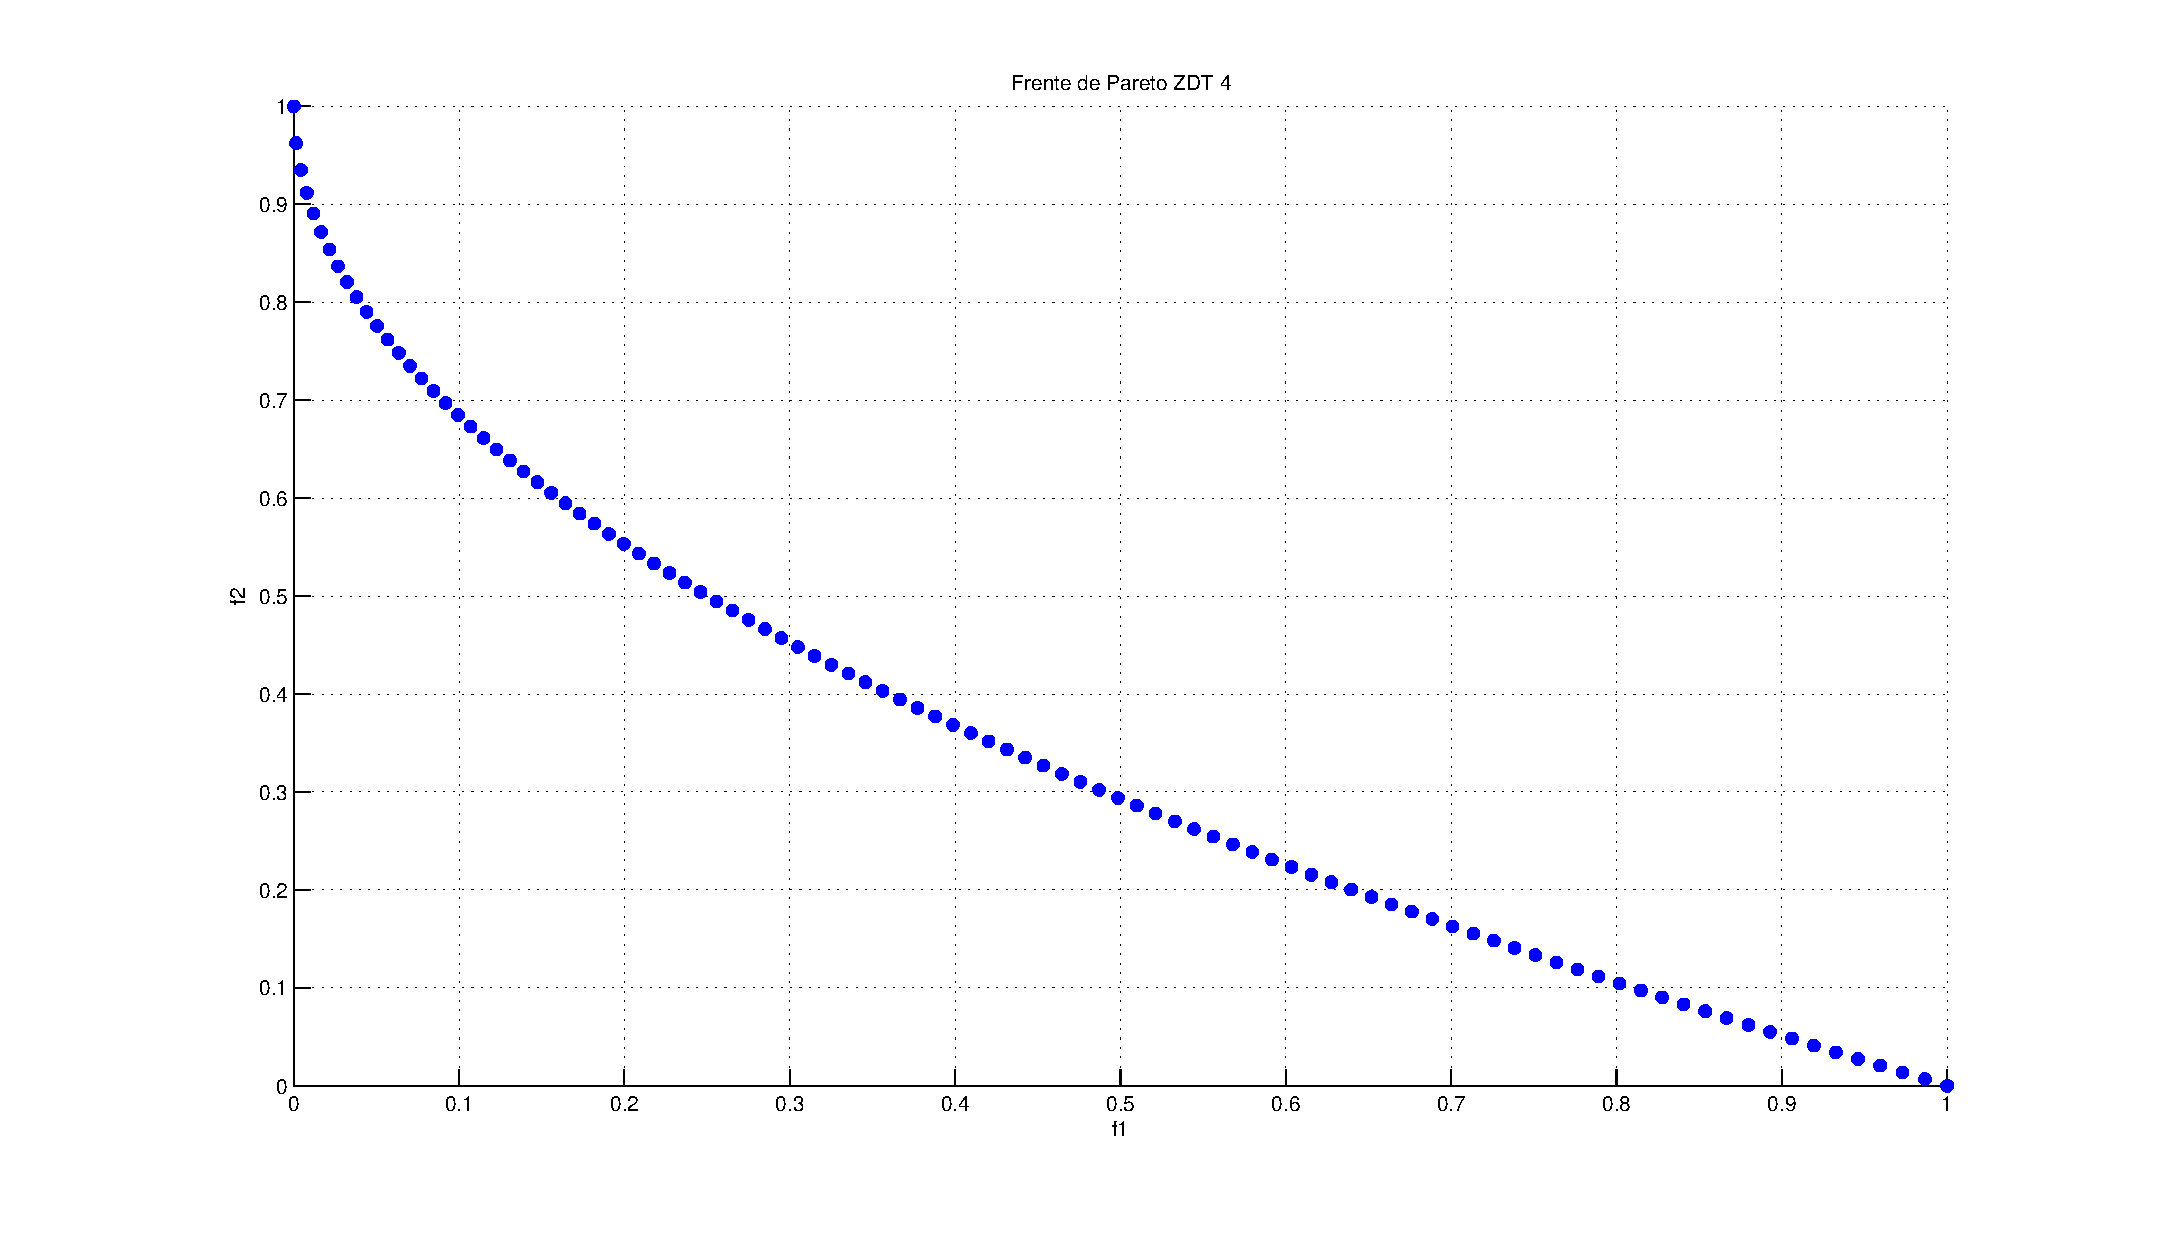
\includegraphics[scale=0.45]{ApendiceA/paretoZDT4.eps}
\caption{Frente de Pareto ZDT4}
\label{fig:ZDT4}
\end{figure} 

\textbf{Formulaci\'on de ZDT6:}

\begin{align*}
f_1(x)&=1- e^{(-4\cdot x_1)} \cdot \sin^6(6\cdot\pi\cdot x_1),\\
f_2(x,g(x))&=g(x)\cdot(1-\left(\frac{f_1}{g(x)}\right)^2),\\
g(x)&=1+9\cdot\left[\frac{\sum_{i=2}^n}{9}\right]^{0.25}
\end{align*}

donde $n=10$, $x_1\in[0,1]$ y $x_i \in[-5,5]$ con $i= 2, \ldots, n$. El \textit{frente de Pareto real} ($\mathcal{F}_{real}$) se forma con $g(x)=1$
y se muestra en la figura \ref{fig:ZDT6}. El espacio de b\'usqueda no es uniforme, tiene una baja densidad en las soluciones cerca del 
$\mathcal{F}_{real}$ y una alta densidad lejos del mismo.

\begin{figure}[h!]
 \centering
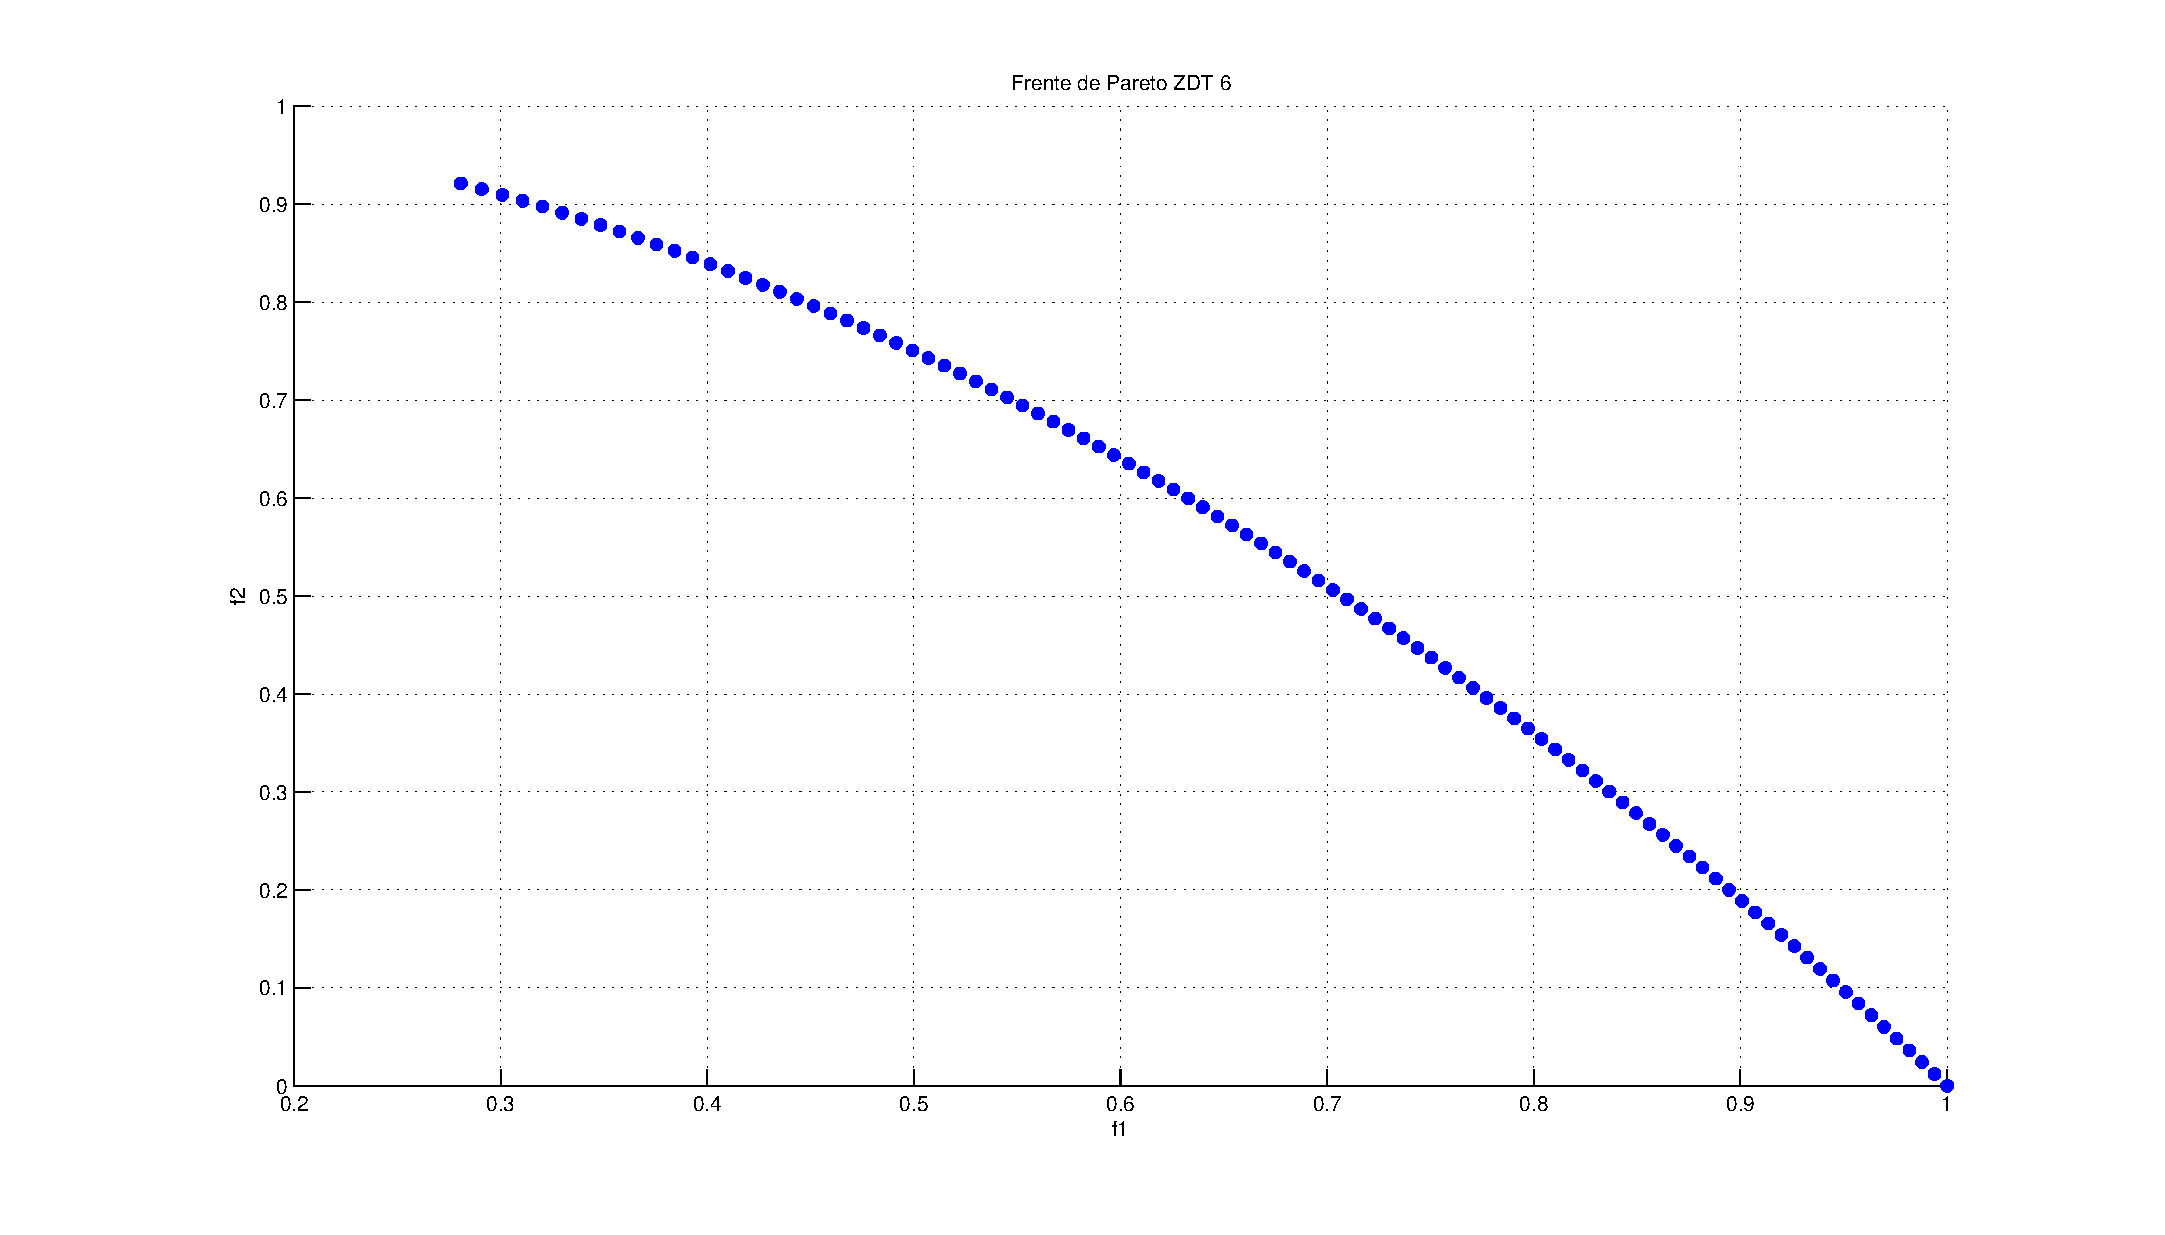
\includegraphics[scale=0.45]{ApendiceA/paretoZDT6.eps}
\caption{Frente de Pareto ZDT6}
\label{fig:ZDT6}
\end{figure} 

\section*{DTLZ (Deb-Thiele-Laumanns-Zitzler)} 

\textbf{Formulaci\'on de DTLZ1:}

\begin{align*}
f_1(x)&=\frac{1}{2}\cdot x_1\cdot x_2 \cdot \ldots \cdot x_{M-1} \cdot (1+g(x))\\
f_2(x)&=\frac{1}{2}\cdot x_1\cdot x_2 \cdot \ldots \cdot(1-x_{M-1})\cdot(1+g(x))\\
\vdots&\\
f_M(x)&=\frac{1}{2}\cdot(1-x_1)\cdot(1+g(x))\\
g(x)&=100\cdot[k+\sum_{i=M}^n(x_i-0.5)^2-cos(20\cdot\pi\cdot(x_i-0.5))]
\end{align*}

donde $n=M+k-1$ (se sugiere un $k=5$) y $x_i\in[0,1]$ con $i = 1, \ldots, n$. El \textit{frente de Pareto real} ($\mathcal{F}_{real}$) para $M=3$ se muestra
en la figura \ref{fig:DTLZ1}. Este problema tiene un {\it frente de Pareto}  lineal, separable y multimodal. El espacio de b\'usqueda 
contiene $11^k-1$ frentes locales. 

\begin{figure}[h!]
 \centering
\includegraphics[scale=0.4]{ApendiceA/paretoDTLZ1.eps}
\caption{Frente de Pareto DTLZ1}
\label{fig:DTLZ1}
\end{figure}

\textbf{Formulaci\'on de DTLZ2:}

\begin{align*}
f_1(x)&=\cos(x_1\frac{\pi}{2})\cdot\cos(x_2\frac{\pi}{2})\cdot\ldots\cdot\cos(x_{M-1}\frac{\pi}{2})\cdot(1+g(x))\\
f_2(x)&=\cos(x_1\frac{\pi}{2})\cdot\cos(x_2\frac{\pi}{2})\cdot\ldots\cdot\sin(x_{M-1}\frac{\pi}{2})\cdot(1+g(x))\\
f_3(x)&=\cos(x_1\frac{\pi}{2})\cdot\cos(x_2\frac{\pi}{2})\cdot\ldots\cdot\sin(x_{M-2}\frac{\pi}{2})\cdot(1+g(x))\\
\vdots&\\
f_{M-1}(x)&=\cos(x_1\frac{\pi}{2})\cdot\sin(x_2\frac{\pi}{2})(1+g(x))\\
f_{M}(x)&=\sin(x_1\frac{\pi}{2})\cdot(1+g(x))\\
g(x)&=\sum_i=(x_i-0.5)^2
\end{align*}

donde $n=M+k-1$ (se sugiere un $k=10$) y $x_i\in[0,1]$ con $i= 1, \ldots, n$. El \textit{frente de Pareto real} ($\mathcal{F}_{real}$)
para $M=3$ se muestra en la figura \ref{fig:DTLZ2}. Tiene un {\it frente de Pareto}  c\'oncavo. Este problea se puede utilizar para 
investigar la habilidad de escalabilidad en objetivos de un algoritmo evolutivo multi-objetivo.

\begin{figure}[h!]
 \centering
\includegraphics[scale=0.4]{ApendiceA/paretoDTLZ2.eps}
\caption{Frente de Pareto DTLZ2}
\label{fig:DTLZ2}
\end{figure}

\textbf{Formulaci\'on de DTLZ3}

\begin{align*}
f_1(x)&=\cos(x_1\frac{\pi}{2})\cdot\cos(x_2\frac{\pi}{2})\cdot\ldots\cdot \cos(x_{M-1}\frac{\pi}{2})\cdot(1+g(x))\\
f_2(x)&=\cos(x_1\frac{\pi}{2})\cdot\cos(x_2\frac{\pi}{2})\cdot\ldots\cdot \sin(x_{M-1}\frac{\pi}{2})\cdot(1+g(x))\\
f_3(x)&=\cos(x_1\frac{\pi}{2})\cdot\cos(x_2\frac{\pi}{2})\cdot\ldots\cdot \sin(x_{M-2}\frac{\pi}{2})\cdot(1+g(x))\\
\vdots&\\
f_{M-1}(x)&=\cos(x_1\frac{\pi}{2})\cdot\sin(x_2\frac{\pi}{2})\cdot(1+g(x))\\
f_{M}(x)&=\sin(x_1\frac{\pi}{2})\cdot (1+g(x))\\
g(x)&=100\cdot [k+\sum_{i=M}^n(x_i-0.5)^2-\cos(20\cdot\pi\cdot(x_i-0.5))]
\end{align*}


donde $n=M+k-1$ (se sugiere un $k=10$) y $x_i\in[0,1]$ con $i=1, \ldots, n$. La funci\'on $g(x)$ introduce  $3\cdot k-1$ frentes locales 
paralelos al frente global. El \textit{frente de Pareto real} ($\mathcal{F}_{real}$) para $M=3$ se muestra en la figura \ref{fig:DTLZ3}.
Tiene un {\it frente de Pareto}  c\'oncavo y multimodal. Este problema prueba la habilidad de un algoritmo evolutivo multi-objetivo de converger al 
$\mathcal{F}_{real}$.

\begin{figure}[h!]
 \centering
\includegraphics[scale=0.4]{ApendiceA/paretoDTLZ3.eps}
\caption{Frente de Pareto DTLZ3}
\label{fig:DTLZ3}
\end{figure}

\textbf{Formulaci\'on de DTLZ4}

\begin{align*}
f_1(x)&=\cos(x_1^\alpha\frac{\pi}{2})\cdot\cos(x_2^\alpha\frac{\pi}{2})\cdot\ldots\cdot cos(x_{M-1}^\alpha\frac{\pi}{2})\cdot(1+g(x))\\
f_2(x)&=\cos(x_1^\alpha\frac{\pi}{2})\cdot\cos(x_2^\alpha\frac{\pi}{2})\cdot\ldots\cdot sin(x_{M-1}^\alpha\frac{\pi}{2})\cdot(1+g(x))\\
f_3(x)&=\cos(x_1^\alpha\frac{\pi}{2})\cdot\cos(x_2^\alpha\frac{\pi}{2})\cdot\ldots\cdot sin(x_{M-2}^\alpha\frac{\pi}{2})\cdot(1+g(x))\\
\vdots&\\
f_{M-1}(x)&=\cos(x_1^\alpha\frac{\pi}{2})\cdot\sin(x_2^\alpha\frac{\pi}{2})\cdot(1+g(x))\\
f_{M}(x)&=\sin(x_1^\alpha\frac{\pi}{2})\cdot(1+g(x))\\
g(x)&=\sum_i(x_i-0.5)^2
\end{align*}


donde $n=M+k-1$ (se sugiere $k=10$ y $\alpha=100$) y $x_i\in[0,1]$ con $i=1,\ldots, n$. El \textit{frente de Pareto real} ($\mathcal{F}_{real}$) 
para $M=3$ se muestra en la figura \ref{fig:DTLZ4}. Tiene un {\it frente de Pareto}  c\'oncavo, separable y multimodal. Este probema prueba 
la habilidad de los algoritmos evolutivos multi-objetivo de mantener una buena distribuci\'on de las soluciones.

\begin{figure}[h!]
 \centering
\includegraphics[scale=0.4]{ApendiceA/paretoDTLZ4.eps}
\caption{Frente de Pareto DTLZ4}
\label{fig:DTLZ4}
\end{figure}

\textbf{Formulaci\'on de DTLZ5}

\begin{align*}
f_1(x)&=\cos(\theta_1\frac{\pi}{2})\cdot\cos(\theta_2\frac{\pi}{2})\cdot\ldots\cdot \cos(\theta_{M-1}\frac{\pi}{2})\cdot(1+g(x))\\
f_2(x)&=\cos(\theta_1\frac{\pi}{2})\cdot\cos(\theta_2\frac{\pi}{2})\cdot\ldots\cdot \sin(\theta_{M-1}\frac{\pi}{2})\cdot(1+g(x))\\
f_3(x)&=\cos(\theta_1\frac{\pi}{2})\cdot\cos(\theta_2\frac{\pi}{2})\cdot\ldots\cdot \sin(\theta_{M-2}\frac{\pi}{2})\cdot(1+g(x))\\
\vdots&\\
f_{M-1}(x)&=\cos(\theta_1\frac{\pi}{2})\cdot\sin(\theta_2\frac{\pi}{2})\cdot(1+g(x))\\
f_{M}(x)&=\sin(\theta_1\frac{\pi}{2})\cdot(1+g(x))\\
\theta_1&=\frac{\pi}{2}x_1\\
\theta_i&=\frac{\pi}{4\cdot(1+g(x))}(1+2\cdot g(x)\cdot x_i),  \text{para} \hspace{1mm} i=2,3\dots,(M-1)\\
g(x)&=\sum^n_i(x_i-0.5)^2
\end{align*}

donde $n=M+k-1$ (se sugiere un $k=10$) y $x_i\in[0,1]$ con $i = 1,\ldots,n$. El \textit{frente de Pareto real} ($\mathcal{F}_{real}$) 
para $M=3$ se muestra en la figura \ref{fig:DTLZ5}. Este problema tiene un {\it frente de Pareto} curvo.

\begin{figure}[h!]
 \centering
\includegraphics[scale=0.4]{ApendiceA/paretoDTLZ5.eps}
\caption{Frente de Pareto DTLZ5}
\label{fig:DTLZ5}
\end{figure}

\textbf{Formulaci\'on de DTLZ6}

\begin{align*}
f_1(x)&=\cos(\theta_1\frac{\pi}{2})\cdot\cos(\theta_2\frac{\pi}{2})\cdot\ldots\cdot \cos(\theta_{M-1}\frac{\pi}{2})\cdot(1+g(x))\\
f_2(x)&=\cos(\theta_1\frac{\pi}{2})\cdot\cos(\theta_2\frac{\pi}{2})\cdot\ldots\cdot \sin(\theta_{M-1}\frac{\pi}{2})\cdot(1+g(x))\\
f_3(x)&=\cos(\theta_1\frac{\pi}{2})\cdot\cos(\theta_2\frac{\pi}{2})\cdot\ldots\cdot \sin(\theta_{M-2}\frac{\pi}{2})\cdot(1+g(x))\\
\vdots&\\
f_{M-1}(x)&=\cos(\theta_1\frac{\pi}{2})\cdot\sin(\theta_2\frac{\pi}{2})\cdot(1+g(x))\\
f_{M}(x)&=\sin(\theta_1\frac{\pi}{2})\cdot(1+g(x))\\
\theta_1&=\frac{\pi}{2}x_1\\
\theta_i&=\frac{\pi}{4(1+g(x))}(1+2\cdot g(x)\cdot x_i),  \text{para}\hspace{1mm} i=2,3\dots,(M-1)\\
g(x)&=\sum^n_i=(x_i-0.5)^0.1
\end{align*}

donde $n=M+k-1$ (se sugiere un $k=10$) y $x_i\in[0,1]$ con $i=1,\ldots,n$.  El \textit{frente de Pareto real} ($\mathcal{F}_{real}$) para 
$M=3$ se muestra en la figura \ref{fig:DTLZ6}. En este problema se modifica la funci\'on $g(x)$ de DTLZ5 volvi\'endolo m\'as dif\'icil. 
Tiene un {\it frente de Pareto} curvo.

\begin{figure}[h!]
 \centering
\includegraphics[scale=0.4]{ApendiceA/paretoDTLZ6.eps}
\caption{Frente de Pareto DTLZ6}
\label{fig:DTLZ6}
\end{figure}

\textbf{Formulaci\'on de DTLZ7}

\begin{align*}
f_1(x)&=x_1 \\
f_2(x)&=x_2\\
\vdots&\\
f_{M-1}(x)&=x_{M-1}\\
f_{M}(x)&=(1+g(x_M))\cdot h(f_1,f_2,\dots,f_{M-1}g(x))\\
g(x)&=1+\frac{9}{k}\cdot\sum_{i=2}^nx_i\\
h(f_1,f_2,\dots,f_{M-1}g(x))&=M-\sum_{i=1}^{M-1}(\frac{f_i}{1+g(x)}(1+\sin{(3\cdot\pi\cdot f_i)}))
\end{align*}


donde $n=M+k-1$ (se sugiere un $k=20$) y $x_i\in[0,1]$ con $i=1,\ldots,n$. El \textit{frente de Pareto real} ($\mathcal{F}_{real}$) para 
$M=3$ se muestra en la figura \ref{fig:DTLZ7}. Tiene un {\it frente de Pareto} discontinuo. Este problema prueba la habilidad de un \
algoritmo evolutivo multi-objetivo de mantener individuos en las diferentes regiones del {\it frente de Pareto}.

\begin{figure}[h!]
 \centering
\includegraphics[scale=0.4]{ApendiceA/paretoDTLZ7.eps}
\caption{Frente de Pareto DTLZ7}
\label{fig:DTLZ7}
\end{figure}

\end{chapter}




















%\begin{chapter}{Tablas de Resultados}
  
\end{chapter}
%\begin{chapter}{C\'odigos Fuente }
  Escribe el siguiente c\'odigo en un archivo llamado \texttt{mopsohv.cpp}:
  \noindent
  \begin{lstlisting}[style=C]
#include <stdlib.h>
#include <stdio.h>
#include <string.h>
#include <math.h>
#include <time.h>
#include <string.h>
#include "randomlib.h"
#include "indicadorHype.h"
#define popsize      100 /*numero de particulas en la poblacion*/
#define archive_size 100 /*tamano del archivo*/
#define verbose      1
#define printevery   10
#define PI 3.14159265358979
#define RMIN  -1.18e-38
#define acotado 1
int function;    /*codigo de la funcion objetivo */
int maxgen;      /*numero maximo de generaciones */
int optimization;/*optimizacion, 0 minimizacion, 1 maximizacion*/
int maxfun;      /*numero maximo de funciones objetivo */
int maxvar;      /*numero maximo de variables */
double bound = 11.0;
/* valores de las variables de las particulas en el archivo*/
double **archiveVar; 
/* valores de aptitud de las particulas en el archivo */
double **archiveFit; 
/* valores de las variables de las particulas en la poblacion*/
double **popVar;     
/* valores de aptitud de las particulas en la poblacion*/
double **popFit;     
/* valor pBest de las particulas en la poblacion*/
double **pbestsVar;  
/* valor de aptitud pBest de las particulas en la poblacion*/
double **pbestsFit;  
/* velocidad de las particulas en la poblacion*/
double **velocity;   
/* probabilidad de mutacion*/
double pMut = 0.5;   
/* contador de soluciones no dominadas en el archivo*/
unsigned int nondomCtr = 0;  
/* Variables para el calculo de la contribucion al hipervolumen */
double *contribution;
double *points;
double *referencePoints;
double *referencePoints_2;
double delta = 10.0;
unsigned int param_k = 1;
double lowerbound = 0.0;
double upperbound;
double volumeT;
double *volumeFit;
double **archiveFit_2;
/**/
void initialize_memory(void);
void free_memory(void);
void initialize_data(unsigned int,unsigned int);
void initialize_rand(void);
void initialize_pop(void);
void initialize_vel(void);
void evaluate(void);
/*funciones prueba*/
double kita_f1(unsigned int);
double kita_f2(unsigned int);
double kursawe_f1(unsigned int);
double kursawe_f2(unsigned int);
double deb_f1(unsigned int);
double deb_f2(unsigned int);
void deb2(unsigned int);
void deb3(unsigned int);
void fonseca2(unsigned int);
double DTLZ6_f1(unsigned int);
double DTLZ6_f2(unsigned int);
double DTLZ6_f3(unsigned int);
void ZDT1(unsigned int);
void ZDT2(unsigned int);
void ZDT3(unsigned int);
void ZDT4(unsigned int);
void ZDT6(unsigned int);
void DTLZ1(unsigned int);
void DTLZ2(unsigned int);
void DTLZ3(unsigned int);
void DTLZ4(unsigned int);
void DTLZ5(unsigned int);
void DTLZ6(unsigned int);
void DTLZ7(unsigned int);
void store_pbests(void);
void insert_nondom(void);
void delete_particle(unsigned int);
unsigned int compare_particles(unsigned int, unsigned int);
unsigned int check_constraints(double *);
void mutate(unsigned int);
void get_ranges(double *, double *);
void maintain_particles(void);
unsigned int compute_gBest(void);
void compute_hvContribution(void);
void compute_velocity(void);
void compute_position(void);
void update_archive(void);
unsigned int check_nondom(unsigned int);
void update_pbests(void);
void save_results(char *);
void qsortFitness(unsigned int, unsigned int, unsigned int);
void qsortHv(unsigned int, unsigned int);
/*inicio del algoritmo principal*/
int main(int argc, char *argv[]){
  char name[20];
  char archiveName[20] = "archive";
  char fitputName[20] = "fitput";
  char varputName[20] = "varput";
  char hvName[20]= "hv";
  unsigned int i, j, t;
  unsigned int fun, gen;
  clock_t  startTime, endTime;
  double duration, clocktime;
  FILE *fitfile,*varfile;
/*Parametros iniciales*/
  strcpy(name,argv[1]);
  fun = atoi(argv[2]);
  gen = atoi(argv[3]);
  printf("%s %d %d \n",name,fun,gen);
  initialize_data(fun,gen);
/*Iniciar variables*/
  initialize_memory();
/* Iniciar generador de aleatorios*/
  initialize_rand();
  startTime = clock();
/* Iniciar contador de generaciones*/
  t = 0;
/* Iniciar valores de la poblacion de manera aleatoria*/
  initialize_pop();
/* Calcular velocidad inicial*/
  initialize_vel();
/* Evaluar las particulas de la poblacion*/
  evaluate();
/* Almacenar el pBest inicial (variables and valor de aptitud) de las particulas*/
  store_pbests();
/* Insertar las particulas no domindas de la poblacion en el archivo*/
  insert_nondom();
/*Ciclo Principal*/
  while(t <= maxgen)  {
    clocktime = (clock() - startTime)/(double)CLOCKS_PER_SEC;
    if(verbose > 0 && t%printevery==0 || t == maxgen){
      fprintf(stdout,"Generation %d Time: %.2f sec\n",t,clocktime);
      fflush(stdout);
    }
/* Calcular la nueva velocidad de cada particula en la pooblacion*/
    compute_velocity();
/* Calcular la nueva posicion de cada particula en la poblacion*/
    compute_position();
/* Mantener las particulas en la poblacion de la poblacion en el espacio de busqueda*/
    maintain_particles();
/* Pertubar las particulas en la poblacion*/
    if(t < maxgen * pMut)
      mutate(t);
/* Evaluar las particulas en la poblacion*/
    evaluate();
/* Insertar nuevas particulas no domindas en el archivo*/
    update_archive();
/* Actualizar el pBest de las particulas en la poblacion*/
    update_pbests();
/* Incrementar contador de generaciones*/
    t++;
  }
/* Escribir resultados en el archivo */
  save_results(strcat(strcat(archiveName,name),".out"));
  endTime = clock();
  duration = ( endTime - startTime ) / (double)CLOCKS_PER_SEC;
  fprintf(stdout, "%lf sec\n", duration);
  free_memory();
  return EXIT_SUCCESS;
}

void initialize_data(unsigned int fun,unsigned int mg){
  function = fun; /*funcion prueba*/
  maxgen = mg; /* numero maximo de generaciones */
  switch(fun){
    case 100: /* Kita */
      maxfun = 2; maxvar = 2; optimization = 1; break;
    case 200: /* Kursawe */
      maxfun = 2; maxvar = 3; optimization = 0; break;
    case 300: /* Deb 1 */
      maxfun = 2; maxvar = 2; optimization = 0; break;
    case 350: /* Deb 2 */
      maxfun = 2; maxvar = 2; optimization = 0; break;
    case 400: /* Deb 3 */
      maxfun = 2; maxvar = 2; optimization = 0; break;
    case 450: /* Fonseca 2 */
      maxfun = 2; maxvar = 2; optimization = 0; break;
    case 500: /* DTLZ7 */
      maxfun = 3; maxvar = 22; optimization = 0; break;
    case 600: /* zdt1 */
      maxfun = 2; maxvar = 30; optimization = 0; break;
    case 605: /* zdt2 */
      maxfun = 2; maxvar = 30; optimization = 0; break;
    case 610: /* zdt3 */
      maxfun = 2; maxvar = 30; optimization = 0; break;
    case 615: /* zdt4 */
      maxfun = 2; maxvar = 10; optimization = 0; break;
    case 620: /* zdt6 */
      maxfun = 2; maxvar = 10; optimization = 0; break;
    case 700: /* DTLZ1*/
      maxfun = 3; maxvar = 7; optimization = 0; break;
    case 705: /* DTLZ2*/
      maxfun = 3; maxvar = 12; optimization = 0; break;
    case 710: /* DTLZ3*/
      maxfun = 3; maxvar = 12; optimization = 0; break;
    case 715: /* DTLZ4*/
      maxfun = 3; maxvar = 12; optimization = 0; break;
    case 720: /* DTLZ5*/
      maxfun = 3; maxvar = 12; optimization = 0; break;
    case 725: /* DTLZ6*/
      maxfun = 3; maxvar = 12; optimization = 0; break;
    case 730: /* DTLZ7*/
      maxfun = 3; maxvar = 22; optimization = 0; break;
/** Agregar mas aqui ***/
  }
}
void initialize_memory(){
  unsigned int i, j;
  /*reservando Memoria*/
  archiveVar = (double **) calloc(archive_size,sizeof(double *));
  archiveFit = (double **) calloc(archive_size,sizeof(double *));
  archiveFit_2 = (double **) calloc(archive_size,sizeof(double *));
  for(i=0;i < archive_size;i++) {
    archiveVar[i] = (double *) calloc(maxvar,sizeof(double));
    archiveFit[i] = (double *) calloc(maxfun,sizeof(double));
    archiveFit_2[i] = (double *) calloc(maxfun,sizeof(double));	
  }
  popVar = (double **) calloc(popsize,sizeof(double *));
  popFit = (double **) calloc(popsize,sizeof(double *));
  pbestsVar = (double **) calloc(popsize,sizeof(double *));
  pbestsFit = (double **) calloc(popsize,sizeof(double *));
  velocity = (double **) calloc(popsize,sizeof(double *));
  for(i=0;i < popsize;i++)  {
    popVar[i] = (double *) calloc(maxvar,sizeof(double));
    pbestsVar[i] = (double *) calloc(maxvar,sizeof(double));
    velocity[i] = (double *) calloc(maxvar,sizeof(double));
  }
  for(i=0;i < popsize;i++) {
    popFit[i] = (double *) calloc(maxfun,sizeof(double));
    pbestsFit[i] = (double *) calloc(maxfun,sizeof(double));
  }
  referencePoints = (double *) calloc(maxfun,sizeof(double));
  referencePoints_2 = (double *) calloc(maxfun,sizeof(double));
  contribution = (double *)calloc(archive_size,sizeof(double));
  points = (double *)calloc(archive_size * maxfun,sizeof(double));  
}

void free_memory(){
  int i;
  for(i=0;i < archive_size;i++) {
    free(archiveVar[i]);
    free(archiveFit[i]);
    free(archiveFit_2[i]);
  }
  free(archiveVar);
  free(archiveFit);
  free(archiveFit_2);
  for(i=0;i < popsize;i++){
    free(popVar[i]);
    free(pbestsVar[i]);
    free(velocity[i]);
  }
  for(i=0;i < popsize;i++){
    free(popFit[i]);
    free(pbestsFit[i]);
  }
  free(popVar);
  free(popFit);
  free(pbestsVar);
  free(pbestsFit);
  free(velocity);
  free(referencePoints);
  free(referencePoints_2);
  free(volumeFit);
  free(points);
  free(contribution);
}

void initialize_rand(){ /*Iniciando el generador de aleatorios randomlib.h */
  unsigned int i, j;
  srand((unsigned int)time((time_t *)NULL));
  i = (unsigned int) (31329.0 * rand() / (RAND_MAX + 1.0));
  j = (unsigned int) (30082.0 * rand() / (RAND_MAX + 1.0));
  RandomInitialise(i,j);
}

void initialize_pop(){ /* Iniciando la poblacion */
  unsigned int i, j;
  switch(function){
  case 100: /* Kita */
    for(i=0; i < popsize; i++)
      for(j =0; j < maxvar; j++)
	popVar[i][j] = RandomDouble(0.0, 7.0);
    break;
  case 200: /* Kursawe */
    for(i=0; i < popsize; i++)
      for(j =0; j < maxvar; j++)
	popVar[i][j] = RandomDouble(-5.0, 5.0);
    break;
  case 300: /* Deb 1 */
    for(i=0; i < popsize; i++)
      for(j =0; j < maxvar; j++)
	popVar[i][j] = RandomDouble(0.1, 0.8191);
    break;
  case 350: /* Deb 2 */
    for(i=0; i < popsize; i++)
      for(j =0; j < maxvar; j++)
	popVar[i][j] = RandomDouble(0.0, 1.0);// 0.8191);
    break;
  case 400: /* Deb 3 */
    for(i=0; i < popsize; i++)
      for(j =0; j < maxvar; j++)
	popVar[i][j] = RandomDouble(0.0, 1.0);
    break;
  case 450: /* Fonseca 2 */
    for(i=0; i < popsize; i++)
      for(j =0; j < maxvar; j++)
	popVar[i][j] = RandomDouble(-4.0, 4.0);
    break;
  case 500: /* DTLZ6 */
    for(i=0; i < popsize; i++)
      for(j =0; j < maxvar; j++)
	popVar[i][j] = RandomDouble(0.0, 1.0);
    break;
  case 600: /* zdt1 */
    for(i=0; i < popsize; i++)
      for(j =0; j < maxvar; j++)
	popVar[i][j] = RandomDouble(-0.0, 1.0);
    break;
  case 605: /* zdt2 */
    for(i=0; i < popsize; i++)
      for(j =0; j < maxvar; j++)
	popVar[i][j] = RandomDouble(0.0, 1.0);
    break;
  case 610: /* zdt3 */
    for(i=0; i < popsize; i++)
      for(j =0; j < maxvar; j++)
	popVar[i][j] = RandomDouble(0.0, 1.0);
    break;
  case 615: /* zdt4 */
    for(i=0; i < popsize; i++){
      popVar[i][0] = RandomDouble(0.0, 1.0);
      for(j =1; j < maxvar; j++)
	popVar[i][j] = RandomDouble(-5.0, 5.0);
    }
    break;
  case 620: /* zdt6 */
    for(i=0; i < popsize; i++)
      for(j =0; j < maxvar; j++)
	popVar[i][j] = RandomDouble(0.0, 1.0);
    break;
  case 700: /* dtlz1 */
    for(i=0; i < popsize; i++)
      for(j =0; j < maxvar; j++)
	popVar[i][j] = RandomDouble(0.0, 1.0);
    break;
  case 705: /* dtlz2 */
    for(i=0; i < popsize; i++)
      for(j =0; j < maxvar; j++)
	popVar[i][j] = RandomDouble(0.0, 1.0);
    break;
  case 710: /* dtlz3 */
    for(i=0; i < popsize; i++)
      for(j =0; j < maxvar; j++)
	popVar[i][j] = RandomDouble(0.0, 1.0);
    break;
  case 715: /* dtlz4 */
    for(i=0; i < popsize; i++)
      for(j =0; j < maxvar; j++)
	popVar[i][j] = RandomDouble(0.0, 1.0);
    break;
  case 720: /* dtlz5 */
    for(i=0; i < popsize; i++)
      for(j =0; j < maxvar; j++)
	popVar[i][j] = RandomDouble(0.0, 1.0);
    break;
  case 725: /* dtlz6 */
    for(i=0; i < popsize; i++)
      for(j =0; j < maxvar; j++)
	popVar[i][j] = RandomDouble(0.0, 1.0);
    break;
  case 730: /* dtlz7 */
    for(i=0; i < popsize; i++)
      for(j =0; j < maxvar; j++)
	popVar[i][j] = RandomDouble(0.0, 1.0);
    break;
   /* Agregar maa aqui */
  }
}

void initialize_vel(){ /*Velocidad inicial*/
  unsigned int i, j;
  for(i = 0; i < popsize; i++)
    for(j = 0; j < maxvar; j++)
      velocity[i][j] = 0.0;
}

void evaluate(){ /*Evaluar las particulas de la poblacion*/
  unsigned int i, j;
  for(i = 0; i < popsize; i++){
    for(j = 0; j < maxfun; j++){
      switch(function + j){
	case 100:	/* Kita's primer objetivo */
	  popFit[i][j] = kita_f1(i); break;
	case 101:	/* Kita's segundo objetivo */
	  popFit[i][j] = kita_f2(i);  break;
	case 200:	/* Kursawe's primer objetivo */
	  popFit[i][j] = kursawe_f1(i); break;
	case 201:	/* Kursawe's segundo objetivo */
	  popFit[i][j] = kursawe_f2(i); break;
	case 300:	/* Deb's primer objetivo */
	  popFit[i][j] = deb_f1(i); break;
	case 301:	/* Deb's segundo objetivo */
	  popFit[i][j] = deb_f2(i);  break;
	case 350: deb2(i); break;
	case 400: deb3(i); break;
        case 450: fonseca2(i); break;
	case 500:	/* DTLZ6's primer objetivo */
	  popFit[i][j] = DTLZ6_f1(i); break;
	case 501:	/* DTLZ6's segundo objetivo */
	  popFit[i][j] = DTLZ6_f2(i); break;
	case 502:	/* DTLZ6's tercer objetivo */
	  popFit[i][j] = DTLZ6_f3(i); break;
        case 600: ZDT1(i); break;
        case 605: ZDT2(i); break;
        case 610: ZDT3(i); break;
        case 615: ZDT4(i); break;
        case 620: ZDT6(i); break;
        case 700: DTLZ1(i); break;
        case 705: DTLZ2(i); break;
        case 710: DTLZ3(i); break;
        case 715: DTLZ4(i); break;
        case 720: DTLZ5(i); break;
        case 725: DTLZ6(i); break;
        case 730: DTLZ7(i); break;
	/*Agregar mas aqui*/
      }/* end of switch */
    }
  }
}

void store_pbests(){ /* Almacenar pBest (variables y valores de fitness) */
  unsigned int i, j;
/* Alamcenar los valores de las variable */
  for(i=0; i < popsize; i++)
    for (j = 0; j < maxvar; j++)
      pbestsVar[i][j] = popVar[i][j];
/* Almacenar el fitness */
  for(i=0; i < popsize; i++)
    for (j = 0; j < maxfun; j++)
      pbestsFit[i][j] = popFit[i][j];
  for (j = 0; j < maxfun; j++)
    referencePoints_2[j]=RMIN;
}

void insert_nondom(){ /* Insertar particulas no dominadas en el archivo */
  unsigned int i, j, k, total, insertFlag, bottom, cont;
  double archiveCons[maxvar], popCons[maxvar];
  for(i=0; i< popsize; i++){
    if(nondomCtr == 0){ /* Si el archivo esta vacio insertar la particula en el archivo */
      for(j = 0; j < maxvar; j++)
	archiveVar[nondomCtr][j] = popVar[i][j];
      for(j = 0; j < maxfun; j++)
	archiveFit[nondomCtr][j] = popFit[i][j];
      nondomCtr += 1;
    }
    else{ /* Si el archivo no esta vacio */
      insertFlag = 1;
      /*Para cada particula en el archivo */
      for(k=0; k < nondomCtr; k++){
      /* Primero, verificar si es factibe */
	for(j=0; j < maxvar; j++){
	  popCons[j] = popVar[i][j];
	  archiveCons[j] = archiveVar[k][j];
	}
      /* Si ambas partculas no son factibles */
	if((check_constraints(archiveCons) > 0) && (check_constraints(popCons) > 0)){
	  delete_particle(k); /* Eliminar particula del archivo */
	  insertFlag = 0;		/* No insertar la particula en la poblacion */
	  break;
	}
	else if(check_constraints(popCons) > 0){ 
	/* Si la particula de la poblacion en infactible */
	  insertFlag = 0;/* No insertar la particula en la poblacion */
	  break;
	}
	else if(check_constraints(archiveCons) > 0){ 
	/* Si la particula en el archivo es infactible */
	  delete_particle(k); /* Borrar la particula en el archivo  */
	  if((nondomCtr != 0) || (k != nondomCtr-1))
	    k--;
	  continue;
	}
  /* Segundo, verificar dominancia*/
      total = 0;
      cont = 0;
  /* Si ambos son factiblesf, vereficar no diminancia*/
      for(j=0; j < maxfun; j++){
	if(( (popFit[i][j] < archiveFit[k][j]) && (optimization == 0)) || (popFit[i][j] > archiveFit[k][j]) && (optimization == 1))
	  total += 1;
	}
      for(j=0; j < maxfun; j++){
	if( (popFit[i][j] == archiveFit[k][j])){
	  cont ++;     /* No insertar la particula en la poblacion */
          insertFlag = 0;
        }
      }
      if(total == maxfun || cont == maxfun)   /* Si la particula es totalmente dominada     */
        delete_particle(k); /* Borrar particula del archivo*/
      else if(total == 0){  
      /* Si la particula en dominada en el archivo*/
	insertFlag = 0;  /* No insertar la particula en la poblacion */
	break;
      }
    } /* Termina la comparacion de una particula en la poblacion con el archivo */
  }
  /* Insertar la particula si es factible y no dominada */
    if(insertFlag == 1){
    /* Si la memoria no esta llena, insertar particula */
      if (nondomCtr < archive_size){
	for(j = 0; j < maxvar; j++)
	  archiveVar[nondomCtr][j] = popVar[i][j];
	for(j = 0; j < maxfun; j++)
	  archiveFit[nondomCtr][j] = popFit[i][j];
	nondomCtr += 1;
      }
      else
      {
	bottom = (unsigned int)((nondomCtr-1) * 0.90);
	/* Selecionar aleatoriamente un lugar para reemplazar */
	k = RandomInt(bottom, nondomCtr-1);
	/* Insertar nueva particula en el archivo */
	for(j = 0; j < maxvar; j++)
	  archiveVar[k][j] = popVar[i][j];
	  for(j = 0; j < maxfun; j++)
	    archiveFit[k][j] = popFit[i][j];
      }
    }
  } /* Termina la comparacion de particulas de la poblacion en el archivo */
}

void delete_particle(unsigned int k){ /* Eliminar Particula en el archivo */
  unsigned int j;
  /* Si la particula es infactible o la ultima particula del archivo o solo una particula en el archivo */
  if( (nondomCtr == 1) || (k == (nondomCtr-1)) ){
    nondomCtr -= 1;
  }
  else{
  /* mover la ultima particula en el lugar de la particula infactible */
  for(j = 0; j < maxvar; j++)
    archiveVar[k][j] = archiveVar[nondomCtr-1][j];
    for(j = 0; j < maxfun; j++)
      archiveFit[k][j] = archiveFit[nondomCtr-1][j];
      nondomCtr -= 1;
  }
}

unsigned int check_constraints(double *consVar){ /* Verificar restricciones q detereminan la factibilidad*/
  unsigned int violations = 0;
  switch(function)
  {
    case 100: /* Kita  */
    if( 0 < (double)(consVar[0] / 6.0 + consVar[1] - 13.0 / 2.0 ))
      violations++;
    if( 0 < (double)(consVar[0] / 2.0 + consVar[1] - 15.0 / 2.0))
      violations++;
    if( 0 < (double)(5.0 * consVar[0] + consVar[1] - 30.0) )
      violations++;
    return violations;
    /** Agregar mas aqui**/
    default:
      return 0;
  }
}

void compute_hvContribution(){ /*Calcula al gBest conforme a la mejor contribucion*/
  int i, j, k, f, begin;
  double best;
  param_k = 1;
  for(j=0; j < maxfun; j++){
    referencePoints[j] = popFit[0][j];
    for(i=0; i < nondomCtr; i++)
      if(popFit[i][j] > referencePoints[j])
	referencePoints[j] = popFit[i][j];    
  }
  for(j=0; j < maxfun; j++){
    if((referencePoints[j] + delta) > referencePoints_2[j]){
      referencePoints[j] = referencePoints[j] + delta;
      referencePoints_2[j] = referencePoints[j] + delta;
    }
    else
      referencePoints[j]=referencePoints_2[j];        
    }
  if(maxfun > 2){
    upperbound = referencePoints[0];
    for(j=0; j < maxfun; j++)
      if(referencePoints[j] > upperbound)
	upperbound = referencePoints[j];
      referencePoints[0] = lowerbound;
      referencePoints[1] = upperbound + delta;      
    }
  hypeIndicator(contribution,nondomCtr,referencePoints,param_k,points,maxfun);
  /*Ordenar por valores de contribucion al hipervolumen*/
  begin = 0;
  qsortHv(begin, nondomCtr);
}

void compute_velocity(){ /* Calcular la nueva velocidad de cada particula en la poblacion */
  unsigned int i, j, gBest, top;
  compute_hvContribution();
  top = (unsigned int)((nondomCtr-1) * 0.05);
  for(i = 0; i < popsize; i++){
    gBest = RandomInt(0,top);
    for(j = 0; j < maxvar; j++)
      velocity[i][j] = 0.4 * velocity[i][j] + 1.0 * RandomDouble(0.0, 1.0) * (pbestsVar[i][j] - popVar[i][j]) + 1.0 * RandomDouble(0.0, 1.0) * (archiveVar[gBest][j] - popVar[i][j]);
  }
}

void compute_position(){
  unsigned int i, j;
/* Calcular la nueva posicion de las particulas */
  for(i = 0; i < popsize; i++)
    for(j = 0; j < maxvar; j++)
      popVar[i][j] = popVar[i][j] + velocity[i][j];
}

void mutate(unsigned int t){ /* Mutacion de Particulas	 */
  unsigned int i;
  int dimension = 0;
  double minvalue[maxvar], maxvalue[maxvar], minvaluetemp, maxvaluetemp, range;
  double valtemp = 0;
  get_ranges(minvalue,maxvalue);
  for(i=0; i < popsize; i++){
    if(flip(pow(1.0-(double)t / (maxgen * pMut),1.5))){
      dimension = RandomInt(0,maxvar-1);
      range =(maxvalue[dimension] - minvalue[dimension]) * pow(1.0 - (double)t / (maxgen * pMut),1.5) / 2;
      valtemp = RandomDouble(range, -range);
      if(popVar[i][dimension] - range < minvalue[dimension])
	minvaluetemp = minvalue[dimension];
      else
	minvaluetemp = popVar[i][dimension] - range;
      if(popVar[i][dimension] + range > maxvalue[dimension])
	maxvaluetemp = maxvalue[dimension];
      else
	maxvaluetemp = popVar[i][dimension] + range;
	popVar[i][dimension] = RandomDouble(minvaluetemp, maxvaluetemp);
    }
  }
}

void update_archive(){  /* Insertar nuevas particulas no dominadas de la poblacion en el archivo */
  unsigned int i, j, k, bottom, m, l, n, flag, temp, pWorse, cont, begin;
  double tempE, worse;
  if(acotado == 1){
    for(i = 0, n = 0; i < nondomCtr; i++)
      for(j = 0; j < maxfun; j++){
        points[n] = archiveFit[i][j];        
        n++;
      }      
    hypeIndicator(contribution,nondomCtr,referencePoints,param_k,points,maxfun);
    worse = contribution[0];
    pWorse = 0;
    for(i = 1; i < nondomCtr; i++){
      if(contribution[i] < worse){
        worse = contribution[i];
        pWorse = i;
      }
    }
  }
 /* para cada particula en la poblacion */
  for(k = 0; k < popsize; k++){
  /* Si la particula en la poblacion es no dominada */
    if (check_nondom(k) == 1){
/* Si la memoria no esta llena, insertar particula */
    if (nondomCtr < archive_size){
      i = nondomCtr;
      for(j = 0; j < maxvar; j++)
	archiveVar[i][j] = popVar[k][j];
      for(j = 0; j < maxfun; j++)
	archiveFit[i][j] = popFit[k][j];
	nondomCtr += 1;
    }
    else{      /* Calcular hipervolumen */
      if (acotado == 1){                   
        for(j = 0; j < maxvar; j++)
	  archiveVar[pWorse][j] = popVar[k][j];
        for(j = 0; j < maxfun; j++)
          archiveFit[pWorse][j] = popFit[k][j];
        for(i = 0, n = 0; i < nondomCtr; i++)
          for(j = 0; j < maxfun; j++){
            points[n] = archiveFit[i][j];
            n++;
          }
        hypeIndicator(contribution,nondomCtr,referencePoints,param_k,points,maxfun);
        worse= contribution[0];
        pWorse = 0;
        for(i = 1; i < nondomCtr; i++){
          if(contribution[i] < worse){
            worse = contribution[i];
            pWorse = i;
          }
        }          
      }
      else{
        bottom = (unsigned int)((nondomCtr-1) * 0.90);
        /* Selecionar aleatoriamente un lugar para reemplazar */
        l = RandomInt(bottom, nondomCtr-1);
        for(j = 0; j < maxvar; j++)
	  archiveVar[l][j] = popVar[k][j];
        for(j = 0; j < maxfun; j++)
          archiveFit[l][j] = popFit[k][j];
	}
      }
    }		
  }
  if(function == 620)
  for(i = 0; i < nondomCtr; i++){
    if(archiveVar[i][1] > 1.0){
      for(j = 0; j < maxvar; j++)
	archiveVar[i][j] = archiveVar[nondomCtr-1][j];
      for(j = 0; j < maxfun; j++)
	archiveFit[i][j] = archiveFit[nondomCtr-1][j];
        nondomCtr -= 1;
    }
  }
}

unsigned int check_nondom(unsigned int i){ /* factibilidad y dominancia de las particulas*/
  unsigned int sum, h = 0, j;
  double archiveCons[maxvar], popCons[maxvar];
  do{
    sum = 0;
    for(j=0; j < maxvar; j++){
      archiveCons[j] = archiveVar[h][j];
      popCons[j] = popVar[i][j];
    }
    /* Si la particula en el archivo tiene menos restricciones violadas */
    if(check_constraints(archiveCons) < check_constraints(popCons))
      return 0;
    /* Si la particula tiene mas restriccion, eliminar*/
    if(check_constraints(archiveCons) > check_constraints(popCons)){
      for(j = 0; j < maxvar; j++)
	archiveVar[h][j] = archiveVar[nondomCtr-1][j];
      for(j = 0; j < maxfun; j++)
	archiveFit[h][j] = archiveFit[nondomCtr-1][j];
	nondomCtr -= 1;
    }
    else{ /*Si tienen las mismas violacion de restricciones*/
      for(j = 0; j < maxfun; j++){
	if( ((archiveFit[h][j] < popFit[i][j]) && (optimization == 0)) || ((archiveFit[h][j] > popFit[i][j]) && (optimization == 1)))
          sum += 1;
      }
      if(sum == maxfun)	/* Si la particula en el archio es dominada */
	return 0;
      else if(sum == 0){
      /* Si la particula en el archivo es domianda borrar */
	for(j = 0; j < maxvar; j++)
	  archiveVar[h][j] = archiveVar[nondomCtr-1][j];
	for(j = 0; j < maxfun; j++)
	  archiveFit[h][j] = archiveFit[nondomCtr-1][j];
	  nondomCtr -= 1;
      }
      else
	h += 1;	
    }
  } while(h < nondomCtr);
  return 1;
}

void get_ranges(double *minvalue,double *maxvalue){ /* Obtener rango de valores de las variables */
  unsigned int i;
  switch (function){
    case 100:	/* Kita */
      for(i = 0; i < maxvar; i++){
	minvalue[i] = 0.0; maxvalue[i] = 7.0;
      }
      break;
    case 200:   /* Kursawe */
      for(i = 0; i < maxvar; i++){
	minvalue[i] = -5.0; maxvalue[i] = 5.0;
      }
      break;
    case 300:
      for(i = 0; i < maxvar; i++){
	minvalue[i] = 0.1; maxvalue[i] = 0.8191;
      }
      break;
    case 350: case 400:	/* Deb 2*/
      for(i = 0; i < maxvar; i++){
	minvalue[i] = 0.0; maxvalue[i] = 1.0;
      }
      break;
    case 450:	/* Fonseca 2 */
      for(i = 0; i < maxvar; i++){
	minvalue[i] = -4.0; maxvalue[i] = 4.0;
      }
      break;
    case 500:	/* DTLZ6 */
      for(i = 0; i < maxvar; i++){
	minvalue[i] = 0.0; maxvalue[i] = 1.0;
      }
      break;
    case 600: case 605: case 610: /* zdt*/
      for(i = 0; i < maxvar; i++){
	minvalue[i] = -0.0; maxvalue[i] = 1.0;
      }
      break;
    case 615: /*zdt4*/
      minvalue[0] = 0.0; maxvalue[0] = 1.0;
      for(i=1; i < maxvar; i++)	{
	minvalue[i] = -5.0; maxvalue[i] =  5.0;
      }
      break;
    case 620:	/* zdt6*/
      for(i = 0; i < maxvar; i++){
	minvalue[i] = 0.0; maxvalue[i] = 1.0;
      }
      break;
    case 700: case 705: case 710: case 715: case 720:	/* dtlz*/
    case 725: case 730:
      for(i = 0; i < maxvar; i++){
	minvalue[i] = 0.0; maxvalue[i] = 1.0;
      }
      break;
  }
}

void maintain_particles(){  /* Mantener las particulas de la poblacion en el espacio de busqueda */
  unsigned int i, j;
  double minvalue[maxvar], maxvalue[maxvar];
  /* Verifica la estabilidad de la poblacion al mantener las partículas en sus fronteras */
  switch (function){
  case 100: /* Kita */
    for(i = 0; i < maxvar; i++){
      minvalue[i] = 0.0; maxvalue[i] = 7.0;
    }
    break;
  case 200: /* Kursawe */
    for(i = 0; i < maxvar; i++){
      minvalue[i] = -5.0; maxvalue[i] = 5.0;
    }
    break;
  case 300:
    for(i = 0; i < maxvar; i++){
      minvalue[i] = 0.1; maxvalue[i] = 0.8191;
    }
    break;
  case 350: case 400:/* Deb */
    for(i = 0; i < maxvar; i++){
      minvalue[i] = 0.0; maxvalue[i] = 1.0;
    }
    break;
  case 450:	/* Fonseca 2 */
    for(i = 0; i < maxvar; i++){
      minvalue[i] = -4.0; maxvalue[i] = 4.0;
    }
    break;
  case 500: /* DTLZ6 */
    for(i = 0; i < maxvar; i++)	{
      minvalue[i] = 0.0; maxvalue[i] = 1.0;
    }
    break;
  case 600: case 605: case 610: /* zdt*/
    for(i = 0; i < maxvar; i++){
      minvalue[i] = -0.0; maxvalue[i] = 1.0;
    }
    break;
  case 615:
    minvalue[0] = 0.0; maxvalue[0] = 1.0;
    for(i=1; i < maxvar; i++) {
      minvalue[i] = -5.0; maxvalue[i] =  5.0;
    }
    break;
  case 620:	/* zdt6*/
    for(i = 0; i < maxvar; i++){
      minvalue[i] = 0.0; maxvalue[i] = 1.0;
    }
    break;
  case 700: case 705: case 710: case 715: case 720:	/* zdt*/
  case 725: case 730:
    for(i = 0; i < maxvar; i++){
      minvalue[i] = 0.0; maxvalue[i] = 1.0;
    }
/* Agregar mas aqui! */
  }
  for(i = 0; i < popsize; i++){
    for(j = 0; j < maxvar; j++){
/* Si la particula se va mas lejos del valor minimo */
      if(popVar[i][j] < minvalue[j]){
  /* HAcer igual al valor minimo */
	popVar[i][j] = minvalue[j];
  /* Cambiar la direccion de manera opuesta */
	velocity[i][j] = -velocity[i][j];
      }
  /* Si la particula se va mas lejos del valor maximo */
      if(popVar[i][j] > maxvalue[j]){
  /* Hacer igual al valor maximo*/
	popVar[i][j] = maxvalue[j];
  /* Cambiar la direccion de manera opuesta */
	velocity[i][j] = -velocity[i][j];
      }
    }
  }
}

void update_pbests(){ /* Actuaizar pBest*/
  unsigned int i,n, j, sum, better;
  for(i = 0; i < popsize; i++){
    sum = 0;
    for(j = 0; j < maxfun; j++){
      if( ((popFit[i][j] < pbestsFit[i][j]) && (optimization == 0)) || ((popFit[i][j] > pbestsFit[i][j]) && (optimization == 1)))
      sum += 1;
    }
    if (sum == maxfun)
      better = 0;    
    else{
      if (sum == 0 )
        better = 1;
      else
        better = RandomInt(0, 1);
    }
    if (better == 0)
    {
      for(j = 0; j < maxfun; j++)
        pbestsFit[i][j] = popFit[i][j];
      for(j = 0; j < maxvar; j++)
        pbestsVar[i][j] = popVar[i][j];
    }
  }
}

void save_results(char *archiveName){  /* Escribir resultados en el archivo */
  unsigned int i, j;
  FILE *fp;
  /* Abrir archivo para escritura */
  fp = fopen(archiveName, "w");
  for(i = 0; i < nondomCtr; i++){
    for(j = 0; j < maxfun; j++)
      fprintf(fp, "%e ", archiveFit[i][j]);
      fprintf(fp, "\n");
  }
  fclose(fp);
}

void qsortFitness(unsigned int f,  unsigned int begin, unsigned int lastPart){
  unsigned int l = begin + 1;
  unsigned int r = lastPart;
  double pivot = archiveFit[begin][f];
  unsigned int k;
  double tempF[maxfun], tempP[maxvar], temp;
  while(l < r){
    if(archiveFit[l][f] <= pivot)
      l++;
    else{
      r--;
      for(k=0; k < maxfun; k++){
        tempF[k] = archiveFit[l][k];
        archiveFit[l][k] = archiveFit[r][k];
      }
      for(k=0; k < maxfun; k++)
	archiveFit[r][k] = tempF[k];
      for(k=0; k < maxvar; k++){
        tempP[k] = archiveVar[l][k];
        archiveVar[l][k] = archiveVar[r][k];
      }
      for(k=0; k<maxvar; k++)
	archiveVar[r][k] = tempP[k];
        temp = contribution[l];
        contribution[l] = contribution[r];
        contribution[r] = temp;
    }
  }
  l--;  
  for(k=0; k<maxfun; k++){
    tempF[k] = archiveFit[begin][k];
    archiveFit[begin][k] = archiveFit[l][k];
  }
  for(k=0; k<maxfun; k++)
    archiveFit[l][k] = tempF[k];  
  for(k=0; k < maxvar; k++){
    tempP[k] = archiveVar[begin][k];
    archiveVar[begin][k] = archiveVar[l][k];
  }
  for(k=0; k < maxvar; k++)
    archiveVar[l][k] = tempP[k];  
  temp = contribution[begin];
  contribution[begin] = contribution[l];
  contribution[l] = temp;
  if(l - begin > 1)
    qsortFitness(f, begin, l);
  if(lastPart - r > 1)
    qsortFitness(f, r, lastPart);
}

void qsortHv(unsigned int begin, unsigned int lastPart){
  unsigned int l = begin + 1;
  unsigned int r = lastPart;
  double pivot = contribution[begin];
  unsigned int k;
  double temp, tempP[maxvar], tempF[maxfun];
  while(l < r){
    if(contribution[l] >= pivot)
      l++;
    else{
      r--;      
      temp = contribution[l];
      contribution[l] = contribution[r];
      contribution[r] = temp;      
      for(k=0; k < maxfun; k++){
        tempF[k] = archiveFit[l][k];
        archiveFit[l][k] = archiveFit[r][k];
      }
      for(k=0; k < maxfun; k++)
	archiveFit[r][k] = tempF[k];      
      for(k=0; k < maxvar; k++){
        tempP[k] = archiveVar[l][k];
        archiveVar[l][k] = archiveVar[r][k];
      }
      for(k=0; k < maxvar; k++)
        archiveVar[r][k] = tempP[k];
    }
  }
  l--;  
  for(k=0; k < maxfun; k++){
    tempF[k] = archiveFit[begin][k];
    archiveFit[begin][k] = archiveFit[l][k];
  }
  for(k=0; k < maxfun; k++)
    archiveFit[l][k] = tempF[k];  
  for(k=0; k < maxvar; k++){
    tempP[k] = archiveVar[begin][k];
    archiveVar[begin][k] = archiveVar[l][k];
  }
  for(k=0; k < maxvar; k++)
    archiveVar[l][k] = tempP[k];  
  temp = contribution[begin];
  contribution[begin] = contribution[l];
  contribution[l] = temp;
  if(l - begin > 1)
    qsortHv(begin, l);
  if(lastPart - r > 1)
    qsortHv(r, lastPart);
}

#include "test-fun.h"

\end{lstlisting}
\noindent
  Escribe el siguiente c\'odigo en un archivo llamado \texttt{test-fun.h}:
  \noindent
  \begin{lstlisting}[style=C]
double kita_f1(unsigned int i){
  return (-(popVar[i][0] * popVar[i][0]) + popVar[i][1] );
}

double kita_f2(unsigned int i){
  return ((popVar[i][0] / 2.0) + popVar[i][1] + 1 );
}

double kursawe_f1(unsigned int i){
  double r = 0.0;
  unsigned int j;
  for(j = 0; j < 2; j++)
    r += -10.0*exp(-0.2*sqrt(pow(popVar[i][j],2)+pow(popVar[i][j+1],2)));
  return r;
}

double kursawe_f2(unsigned int i){
  double r = 0.0;
  unsigned int j;
  for(j = 0; j < 3; j++)
  r += pow(fabs(popVar[i][j]),0.8)+5.0*sin(pow(popVar[i][j],3));
  return r;
}

double deb_f1(unsigned int i){
  return (popVar[i][0]);
}

double deb_f2(unsigned int i){
  double g = 2.0-exp(-pow(((popVar[i][1]-0.2)/0.004),2))-0.8*exp(-pow(((popVar[i][1]-0.6)/0.4),2));
  return ((double)g / popVar[i][0]);
}

double DTLZ6_f1(unsigned int i){
  return (popVar[i][0]);
}

double DTLZ6_f2(unsigned int i)
{
  return (popVar[i][1]);
}

double DTLZ6_f3(unsigned int i){
  unsigned int j = 0;
  unsigned int n = maxvar;
  unsigned int k = n - maxfun + 1;
  double g, h, s, t;
  s = 0;
  for (j = 2; j < maxvar; j++){
    s += popVar[i][j];
  }
  g = 1 + (9 / 20)  * s;
  t = 0;
  for (j = 0; j < maxfun-1; j++){
    t += (popVar[i][j]*(1+sin(3*PI*popVar[i][j])))/(1+g);
  }
  h = 3 - t;
  return ((1 + g) * h);
}

void deb2(unsigned int i) {
  double g;
  double h;
  double f1;
  f1 = popVar[i][0];
  g = 1.0 + 10.0 * popVar[i][1];
  h = 1.0 - pow((f1/g),2.0)-(f1/g)*sin(12.0*PI*f1);
  popFit[i][0] = f1;
  popFit[i][1] = g * h ;
  return;
}

void deb3(unsigned int i){
  double g, h, f1, alfa, beta, seno, argumento, q;
  alfa = 10.0;
  q = 10.0;
  beta = 1.0;
  argumento = q * PI * popVar[i][0];
  seno = sin(argumento);
  f1 = 1.0 - exp(-4.0 * popVar[i][0]) * pow(seno, 4);
  g = 1.0 + popVar[i][1] * popVar[i][1];
  if (f1 <= beta * g){
    h = 1.0 - pow((f1 / (beta * g)), alfa);
  }
  else{
    h = 0.0;
  }
  popFit[i][0] = f1;
  popFit[i][1] = g * h;
  return;
}

void fonseca2(unsigned int i){
  double s1, s2;
  int j;
  s1 = s2 = 0.0;
  for (j = 0; j < maxvar; j++){
    s1 += pow((popVar[i][j] - (1.0 / sqrt((double) maxvar))), 2.0);
    s2 += pow((popVar[i][j] + (1.0 / sqrt((double) maxvar))), 2.0);
  }

	popFit[i][0] = 1.0 - exp(-s1);
	popFit[i][1] = 1.0 - exp(-s2);
	return;
}

void ZDT1(unsigned int i){
  double f1, f2, g, h, sum;
  int j;
  f1 = popVar[i][0];
  sum = 0.0;
  for (j = 1; j < maxvar; j++){
    sum += popVar[i][j];
  }
  g = 1.0 + 9.0 * sum / ((double)maxvar - 1.0);
  h = 1.0 - sqrt(f1 / g);
  f2 = g * h;
  popFit[i][0] = f1;
  popFit[i][1] = f2;
  return;
}

void ZDT2(unsigned int i){
  double f1, f2, g, h, sum;
  int j;
  f1 = popVar[i][0];
  sum = 0.0;
  for (j = 1; j < maxvar; j++){
    sum += popVar[i][j];
  }
  g = 1.0 + 9.0 * sum / ((double)maxvar - 1.0);
  h = 1.0 - pow((f1 / g), 2.0);
  f2 = g * h;
  popFit[i][0] = f1;
  popFit[i][1] = f2;
  return;
}

void ZDT3(unsigned int i){
  double f1, f2, g, h, sum;
  int j;
  f1 = popVar[i][0];
  sum = 0.0;
  for (j = 1; j < maxvar; j++){
    sum += popVar[i][j];
  }
  g = 1.0 + 9.0 * sum / ((double)maxvar - 1.0);
  h = 1.0 - sqrt(f1 / g) - (f1 / g) * sin(10.0 * PI * f1);
  f2 = g * h;
  popFit[i][0] = f1;
  popFit[i][1] = f2;
  return;
}

void ZDT4(unsigned int i){
  double f1, f2, g, h, sum;
  int j;
  f1 = popVar[i][0];
  sum = 0.0;
  for (j = 1; j < maxvar; j++){
    sum += (pow(popVar[i][j], 2.0) - 10.0 * cos(4.0 * PI * popVar[i][j]));
  }
  g = 1.0 + 10.0 * ((double)maxvar - 1.0) + sum;
  h = 1.0 - sqrt(f1 / g);
  f2 = g * h;
  popFit[i][0] = f1;
  popFit[i][1] = f2;
  return;
}

void ZDT6(unsigned int i){
  double f1, f2, g, h, sum;
  int j;
  f1 = 1.0 - exp(-4.0 * popVar[i][0]) * pow(sin(6.0 * PI * popVar[i][0]), 6.0);
  sum = 0.0;
  for (j = 1; j < maxvar; j++){
    sum += popVar[i][j];
  }
  g = 1.0 + 9.0 * pow((sum / ((double)maxvar - 1.0)), 0.25);
  h = 1.0 - pow((f1 / g), 2.0);
  f2 = g * h;
  popFit[i][0] = f1;
  popFit[i][1] = f2;
  popFit[i][1] = f2;
  return;
}

void DTLZ1(unsigned int i){
  int j;
  double sum;
  double g;
  int n = maxvar;
  int m = maxfun;
  int k = n - m + 1
  sum = 0.0;
  for (j = m - 1; j < n; j++){
    sum += pow(popVar[i][j] - 0.5, 2.0) - cos(20.0 * PI * (popVar[i][j] - 0.5));
  }
  g = 100.0 * (k + sum);
  popFit[i][0]= (0.5 * (1.0 + g) * popVar[i][0] * popVar[i][1]);
  popFit[i][1] = 0.5 * (1.0 + g) * (1.0 - popVar[i][1]) * popVar[i][0];
  popFit[i][2] = 0.5 * (1.0 + g) * (1.0 - popVar[i][0]);
  return;
}

void DTLZ2(unsigned int i){
  int j;
  double sum;
  double g;
  int n = maxvar;
  int m = maxfun;
  sum = 0.0;
  for (j = m - 1; j < n; j++){
    sum += pow(popVar[i][j] - 0.5, 2.0);
  }
  g = sum;
  popFit[i][0] = (1.0 + g) * cos(popVar[i][0] * PI * 0.5) * cos(popVar[i][1] * PI * 0.5);
  popFit[i][1] = (1.0 + g) * cos(popVar[i][0] * PI * 0.5) * sin(popVar[i][1] * PI * 0.5);
  popFit[i][2] = (1.0 + g) * sin(popVar[i][0] * PI * 0.5);
  return;
}

void DTLZ3(unsigned int i){
  int j;
  double sum;
  double g;
  int n = maxvar;
  int m = maxfun;
  int k = n - m + 1;
  sum = 0.0;
  for (j = m - 1; j < n; j++){
    sum += pow(popVar[i][j] - 0.5, 2.0) - cos(20.0 * PI * (popVar[i][j] - 0.5));
  }
  g = 100.0 * (k + sum);
  popFit[i][0] = (1.0 + g) * cos(popVar[i][0] * PI * 0.5) * cos(popVar[i][1] * PI * 0.5);
  popFit[i][1] = (1.0 + g) * cos(popVar[i][0] * PI * 0.5) * sin(popVar[i][1] * PI * 0.5);
  popFit[i][2] = (1.0 + g) * sin(popVar[i][0] * PI * 0.5);
  return;
}

void DTLZ4(unsigned int i){
  int j;
  double alpha;
  double g, factor1, factor2;
  int n = maxvar;
  int m = maxfun;
  alpha = 100;
  g = 0.0;
  for (j = m - 1; j < n; j++){
    g += pow(popVar[i][j] - 0.5, 2.0);
  }
  factor1 = pow(popVar[i][0], alpha);
  factor2 = pow(popVar[i][1], alpha);
  popFit[i][0] = (1.0 + g) * cos(factor1 * PI * 0.5) * cos(factor2 * PI * 0.5);
  popFit[i][1] = (1.0 + g) * cos(factor1 * PI * 0.5) * sin(factor2 * PI * 0.5);
  popFit[i][2] = (1.0 + g) * sin(factor1 * PI * 0.5);
  return;
}

void DTLZ5(unsigned int i){
  int j;
  double g;
  double tetha[3];
  int n = maxvar;
  int m = maxfun;
  g = 0.0;
  for (j = m - 1; j < n; j++){
    g += pow(popVar[i][j] - 0.5, 2.0);
  }
  tetha[0] = (PI * 0.5) * popVar[i][0];
  tetha[1] = (PI / (4.0 * (1.0 + g))) * (1.0 + 2.0 * g * popVar[i][1]);
  popFit[i][0] = (1.0 + g) * cos(tetha[0]) * cos(tetha[1]);
  popFit[i][1] = (1.0 + g) * cos(tetha[0]) * sin(tetha[1]);
  popFit[i][2] = (1.0 + g) * sin(tetha[0]);
  return;
}

void DTLZ6(unsigned int i){
  int j;
  double g;
  double tetha[3];
  int n = maxvar;
  int m = maxfun;
  g = 0.0;
  for (j = m - 1; j < n; j++){
    g += pow(popVar[i][j], 0.1);
    }
  tetha[0] = (PI * 0.5) * popVar[i][0];
  tetha[1] = (PI / (4.0 * (1.0 + g))) * (1.0 + 2.0 * g * popVar[i][1]);
  popFit[i][0] = (1.0 + g) * cos(tetha[0]) * cos(tetha[1]);
  popFit[i][1] = (1.0 + g) * cos(tetha[0]) * sin(tetha[1]);
  popFit[i][2] = (1.0 + g) * sin(tetha[0]);
  return;
}

void DTLZ7(unsigned int i){
  int j;
  double sum;
  double g, h;
  int n = maxvar;
  int m = maxfun;
  int k = n - m + 1;
  sum = 0.0;
  for (j = m - 1; j < n; j++){
    sum += popVar[i][j];
  }
  g = 1.0 + (9.0 / (double) k) * sum;
  popFit[i][0] = popVar[i][0];
  popFit[i][1] = popVar[i][1];
  h = m - (((popFit[i][0] / (1.0 + g)) * (1.0 + sin(3.0 * PI * popFit[i][0]))) + ((popFit[i][1]/(1.0 + g)) * (1.0 + sin(3.0 * PI * popFit[i][1]))));
  popFit[i][2] = (1.0 + g) * h;
  return;
}
\end{lstlisting}
\noindent
  Escribe el siguiente c\'odigo en un archivo llamado \texttt{indicadorHype.h}:
  \noindent
  \begin{lstlisting}[style=C]
#include <stdlib.h>
#include <stdio.h>
#include <string.h>
#include <assert.h>
#include <math.h>

int dim;    /* number of objectives */
int weaklyDominates( double *point1, double *point2, int no_objectives);
double drand( double from, double to );
void rearrangeIndicesByColumn(double *mat, int rows, int columns, int col, int *ind);
void hypeExactRecursive( double* input_p, int pnts, int dim, int nrOfPnts,int actDim, double* bounds, int* input_pvec, double* fitness, double* rho, int param_k );
void hypeExact( double* val, int popsize, double *boundsVec,	int param_k, double* points, double* rho);
void hypeSampling( double* val, int popsize, double lowerbound,double upperbound, int nrOfSamples, int param_k, double* points, double* rho );
void hypeIndicator( double* val, int popsize, double *boundsVec, int param_k, double* points);

double drand( double from, double to ){
  double j;
  j = from + (double)( (to-from)*rand() / ( RAND_MAX + 1.0) );
  return (j);
}
int weaklyDominates( double *point1, double *point2, int no_objectives){
  int better;
  int i = 0;
  better = 1;
  while( i < no_objectives && better )
  {
    better = point1[i] <= point2[i];
    i++;
  }
  return better;
}
/* Internal function used by hypeExact */
void rearrangeIndicesByColumn(double *mat, int rows, int columns, int col,int *ind ){
  #define  MAX_LEVELS  300
  int  beg[MAX_LEVELS], end[MAX_LEVELS], i = 0, L, R, swap;
  double pref, pind;
  double ref[rows];
  for( i = 0; i < rows; i++ ) {
    ref[i] = mat[ col + ind[i]*columns ];
  }
  i = 0;
  beg[0] = 0; end[0] = rows;
  while ( i >= 0 ) {
    L = beg[i]; R = end[i]-1;
    if( L < R ) {
      pref = ref[ L ];
      pind = ind[ L ];
      while( L < R ) {
	while( ref[ R ] >= pref && L < R )
	R--;
	if( L < R ) {
	  ref[ L ] = ref[ R ];
	  ind[ L++] = ind[R];
	}
	while( ref[L] <= pref && L < R )
	L++;
	if( L < R) {
	  ref[ R ] = ref[ L ];
	  ind[ R--] = ind[L];	
	}
      }
      ref[ L ] = pref; ind[L] = pind;
      beg[i+1] = L+1; end[i+1] = end[i];
      end[i++] = L;
      if( end[i] - beg[i] > end[i-1] - beg[i-1] ) {
	swap = beg[i]; beg[i] = beg[i-1]; beg[i-1] = swap;
	swap = end[i]; end[i] = end[i-1]; end[i-1] = swap;
      }
    }
    else
      i--;    
  }
}
/* Internal function used by hypeExact */
void hypeExactRecursive( double* input_p, int pnts, int dim, int nrOfPnts,int actDim, double* bounds, int* input_pvec, double* fitness, double* rho, int param_k){
  int i, j;
  double extrusion;
  int pvec[pnts];
  double p[pnts*dim];
  for( i = 0; i < pnts; i++ ) {
    fitness[i] = 0
    pvec[i] = input_pvec[i];
  }
  for( i = 0; i < pnts*dim; i++)
    p[i] = input_p[i];
  rearrangeIndicesByColumn( p, nrOfPnts, dim, actDim, pvec);
  for( i = 0; i < nrOfPnts; i++){
    if( i < nrOfPnts - 1 )
      extrusion = p[ (pvec[i+1])*dim + actDim ] - p[ pvec[i]*dim + actDim ];
    else
      extrusion = bounds[actDim] - p[ pvec[i]*dim + actDim ];
    if(actDim == 0) {
      if(i+1 <= param_k)
	for(j = 0; j <= i; j++) {
	  fitness[pvec[j]] = fitness[pvec[j]]+ extrusion*rho[i+1];
	}
    }
    else if(extrusion > 0) {
      double tmpfit[pnts];
      hypeExactRecursive(p,pnts,dim,i+1,actDim-1,bounds,pvec,tmpfit,rho,param_k);
      for( j = 0; j < pnts; j++ )
	fitness[j] += extrusion*tmpfit[j];
    }
  }
}
/* Calculating the hypeIndicator
  \f[ \sum_{i=1}^k \left( \prod_{j=1}^{i-1} \frac{k-j}{|P|-j} \right) \frac{ Leb( H_i(a) ) }{ i } \f]
*/
void hypeExact( double* val, int popsize,double *boundsVec, int param_k, double* points, double* rho){
  int i, indices[ popsize ];
  for( i = 0; i < popsize; i++  )
    indices[i] = i;
/** Recursively calculate the indicator values */
  hypeExactRecursive(points,popsize,dim,popsize,dim-1,boundsVec,indices,val,rho,param_k);
}

void hypeSampling(double* val, int popsize, double lowerbound,double upperbound, int nrOfSamples, int param_k, double* points, double* rho){
/**Sampling the hypeIndicator
 * \f[ \sum_{i=1}^k \left( \prod_{j=1}^{i-1} \frac{k-j}{|P|-j} \right) \frac{ Leb( H_i(a) ) }{ i } \f]
 * @param[out] val vector of all indicators
 * @param[in] popsize size of the population \f$ |P| \f$
 * @param[in] lowerbound scalar denoting the lower vertex of the sampling box
 * @param[in] upperbound scalar denoting the upper vertex of the sampling box
 * @param[in] nrOfSamples the total number of samples
 * @param[in] param_k the variable \f$ k \f$
 * @param[in] points matrix of all objective values dim*popsize entries
 * @param[in] rho weight coefficients
 * @pre popsize >= 0 && lowerbound <= upperbound && param_k >= 1 && param_k <= popsize
 */
  assert(popsize >= 0 );
  assert( lowerbound <= upperbound );
  assert( param_k >= 1 );
  assert( param_k <= popsize );
  int i, s, k;
  int hitstat[ popsize ];
  int domCount;
  double sample[ dim ];
  for( s = 0; s < nrOfSamples; s++ ) {
    for( k = 0; k < dim; k++ )
    sample[ k ] = drand( lowerbound, upperbound );
    domCount = 0;
    for( i = 0; i < popsize; i++ ){
      if( weaklyDominates( points + (i*dim), sample, dim) ){
	domCount++;
	if( domCount > param_k )
	break;
	hitstat[i] = 1;
      }
      else
	hitstat[i] = 0;
    }
    if( domCount > 0 && domCount <= param_k ){
      for( i = 0; i < popsize; i++ )
	if( hitstat[i] == 1 )
      val[i] += rho[domCount];
    }
  }
  for( i = 0; i < popsize; i++ ){
    val[i] = val[i]*pow((upperbound-lowerbound),dim)/(double)nrOfSamples;
  }
}

void hypeIndicator( double* val, int popsize, double *boundsVec, int param_k, double* points, int dimension){
/** Determine the hypeIndicator
 * \f[ \sum_{i=1}^k \left( \prod_{j=1}^{i-1} \frac{k-j}{|P|-j} \right) \frac{ Leb( H_i(a) ) }{ i } \f]
 * if nrOfSamples < 0, then do exact calculation, else sample the indicator
 * @param[out] val vector of all indicator values
 * @param[in] popsize size of the population \f$ |P| \f$
 * @param[in] lowerbound scalar denoting the lower vertex of the sampling box
 * @param[in] upperbound scalar denoting the upper vertex of the sampling box
 * @param[in] nrOfSamples the total number of samples or, if negative, flag that exact calculation should be used.
 * @param[in] param_k the variable \f$ k \f$
 * @param[in] points matrix of all objective values dim*popsize entries
 * @param[in] rho weight coefficients
 */
  int i,j;
  double rho[param_k + 1];
  double lowerbound, upperbound;
  int nrOfSamples;
  dim = dimension;  
  /** Set alpha */
  rho[0] = 0;
  for( i = 1; i <= param_k; i++ ){
    rho[i] = 1.0 / (double)i;
    for( j = 1; j <= i-1; j++ )
      rho[i] *= (double)(param_k - j ) / (double)( popsize - j );      
    }
  for( i = 0; i < popsize; i++ )
    val[i] = 0.0;
  if( dim < 3 ) {
    hypeExact( val, popsize, boundsVec, param_k, points,rho );
  }
  else  {
    nrOfSamples = 10000;        
    lowerbound = boundsVec[0];
    upperbound = boundsVec[1];
    hypeSampling( val, popsize, lowerbound, upperbound, nrOfSamples,param_k, points, rho);
  }
}

\end{lstlisting}
\noindent
  Escribe el siguiente c\'odigo en un archivo llamado \texttt{randomlib.h}:
  \noindent
  \begin{lstlisting}[style=C]
/******************************************************************
*Random Library, Downloaded at:
*http://www.swin.edu.au/astronomy/pbourke/software/random/
*******************************************************************/
#define FALSE 0
#define TRUE 1
/*
   This Random Number Generator is based on the algorithm in a FORTRAN
   version published by George Marsaglia and Arif Zaman, Florida State
   University; ref.: see original comments below.
   At the fhw (Fachhochschule Wiesbaden, W.Germany), Dept. of Computer
   Science, we have written sources in further languages (C, Modula-2
   Turbo-Pascal(3.0, 5.0), Basic and Ada) to get exactly the same test
   results compared with the original FORTRAN version.
   April 1989
   Karl-L. Noell <NOELL@DWIFH1.BITNET>
      and  Helmut  Weber <WEBER@DWIFH1.BITNET>

   This random number generator originally appeared in "Toward a Universal
   Random Number Generator" by George Marsaglia and Arif Zaman.
   Florida State University Report: FSU-SCRI-87-50 (1987)
   It was later modified by F. James and published in "A Review of Pseudo-
   random Number Generators"
   THIS IS THE BEST KNOWN RANDOM NUMBER GENERATOR AVAILABLE.
   (However, a newly discovered technique can yield
   a period of 10^600. But that is still in the development stage.)
   It passes ALL of the tests for random number generators and has a period
   of 2^144, is completely portable (gives bit identical results on all
   machines with at least 24-bit mantissas in the floating point
   representation).
   The algorithm is a combination of a Fibonacci sequence (with lags of 97
   and 33, and operation "subtraction plus one, modulo one") and an
   "arithmetic sequence" (using subtraction).

   Use IJ = 1802 & KL = 9373 to test the random number generator. The
   subroutine RANMAR should be used to generate 20000 random numbers.
   Then display the next six random numbers generated multiplied by 4096*4096
   If the random number generator is working properly, the random numbers
   should be:
           6533892.0  14220222.0  7275067.0
           6172232.0  8354498.0   10633180.0
*/
/* Globals */
double u[97],c,cd,cm;
int i97,j97;
int test = FALSE;
/*
   This is the initialization routine for the random number generator.
   NOTE: The seed variables can have values between:
   0 <= IJ <= 31328
   0 <= KL <= 30081
   The random number sequences created by these two seeds are of sufficient
   length to complete an entire calculation with. For example, if sveral
   different groups are working on different parts of the same calculation,
   each group could be assigned its own IJ seed. This would leave each group
   with 30000 choices for the second seed. That is to say, this random
   number generator can create 900 million different subsequences -- with
   each subsequence having a length of approximately 10^30.
*/
void RandomInitialise(int ij,int kl){
   double s,t;
   int ii,i,j,k,l,jj,m;
   /*
      Handle the seed range errors
         First random number seed must be between 0 and 31328
         Second seed must have a value between 0 and 30081
   */
   if (ij < 0 || ij > 31328 || kl < 0 || kl > 30081) {
      ij = 1802;
      kl = 9373;
   }
   i = (ij / 177) % 177 + 2;
   j = (ij % 177)       + 2;
   k = (kl / 169) % 178 + 1;
   l = (kl % 169);
   for (ii=0; ii<97; ii++) {
      s = 0.0;
      t = 0.5;
      for (jj=0; jj<24; jj++) {
         m = (((i * j) % 179) * k) % 179;
         i = j;
         j = k;
         k = m;
         l = (53 * l + 1) % 169;
         if (((l * m % 64)) >= 32)
            s += t;
         t *= 0.5;
      }
      u[ii] = s;
   }
   c    = 362436.0 / 16777216.0;
   cd   = 7654321.0 / 16777216.0;
   cm   = 16777213.0 / 16777216.0;
   i97  = 97;
   j97  = 33;
   test = TRUE;
}
/*
   This is the random number generator proposed by George Marsaglia in
   Florida State University Report: FSU-SCRI-87-50
*/
double RandomUniform(void){
   double uni;
   /* Make sure the initialisation routine has been called */
   if (!test)
      RandomInitialise(1802,9373);
   uni = u[i97-1] - u[j97-1];
   if (uni <= 0.0)
      uni++;
   u[i97-1] = uni;
   i97--;
   if (i97 == 0)
      i97 = 97;
   j97--;
   if (j97 == 0)
      j97 = 97;
   c -= cd;
   if (c < 0.0)
      c += cm;
   uni -= c;
   if (uni < 0.0)
      uni++;
   return(uni);
}
/*
  ALGORITHM 712, COLLECTED ALGORITHMS FROM ACM.
  THIS WORK PUBLISHED IN TRANSACTIONS ON MATHEMATICAL SOFTWARE,
  VOL. 18, NO. 4, DECEMBER, 1992, PP. 434-435.
  The function returns a normally distributed pseudo-random number
  with a given mean and standard devaiation.  Calls are made to a
  function subprogram which must return independent random
  numbers uniform in the interval (0,1).
  The algorithm uses the ratio of uniforms method of A.J. Kinderman
  and J.F. Monahan augmented with quadratic bounding curves.
*/
double RandomGaussian(double mean,double stddev){
   double  q,u,v,x,y;
   /*
      Generate P = (u,v) uniform in rect. enclosing acceptance region
      Make sure that any random numbers <= 0 are rejected, since
      gaussian() requires uniforms > 0, but RandomUniform() delivers >= 0.
   */
   do {
      u = RandomUniform();
      v = RandomUniform();
      if (u <= 0.0 || v <= 0.0) {
          u = 1.0;
          v = 1.0;
      }
      v = 1.7156 * (v - 0.5);
      /*  Evaluate the quadratic form */
      x = u - 0.449871;
      y = fabs(v) + 0.386595;
      q = x * x + y * (0.19600 * y - 0.25472 * x);
      /* Accept P if inside inner ellipse */
      if (q < 0.27597)
         break;
      /*  Reject P if outside outer ellipse, or outside acceptance region */
    } while ((q > 0.27846) || (v * v > -4.0 * log(u) * u * u));
    /*  Return ratio of P's coordinates as the normal deviate */
    return (mean + stddev * v / u);
}
/*
   Return random integer within a range, lower -> upper INCLUSIVE
*/
int RandomInt(int lower, int upper){
   return((int)(RandomUniform() * (upper - lower + 1)) + lower);
}
/*
   Return random float within a range, lower -> upper
*/
double RandomDouble(double lower, double upper){
   return((upper - lower) * RandomUniform() + lower);
}
int  flip(double pf){
    if(RandomDouble(0.0,1.0)<=pf)
        return 1;
    else
        return 0;
}
\end{lstlisting}
\noindent
\end{chapter}

 \backmatter

\addcontentsline{toc}{chapter}{Bibliograf�a}
%\bibliographystyle{unsrt}
%\bibliographystyle{plain}
\bibliographystyle{apalike}
\bibliography{biblio.bib}

\end{document}
